\documentclass[12pt]{book}
% setup the page geometry for landscape and use maximum screen real estate
%\usepackage[dvips]{geometry,graphicx,color}
\usepackage[pdftex]{geometry,graphicx,color}
\usepackage{bm}
\usepackage{amsmath}
\usepackage{tensor}
\usepackage{amsfonts}
\usepackage{comment}
\usepackage{srcltx}
\usepackage{amssymb}
\usepackage{rotating}
\usepackage{setspace}
\usepackage{parskip}
\usepackage{hyperref}
\usepackage{eufrak}
\usepackage{mathtools}
\usepackage{tensor}
\usepackage{bbding}
\usepackage{tensor}
\usepackage{pdfpages}
\usepackage{sectsty}
\usepackage{makecell}
\usepackage{longtable}
\usepackage{float}
\usepackage{listings}
\lstloadlanguages{Python}
%\usepackage[hyphens]{url}
\DeclareGraphicsExtensions{.pdf}
\geometry{headsep=2.0em,hscale=0.80}
\newcommand{\ubh}{\bm{\hat{u}}}
\newcommand{\ebh}{\bm{\hat{e}}}
\newcommand{\ebf}{\bm{e}}
%\definecolor{red}{rgb}{1,0,0}
\setlength{\parindent}{0in}
\usepackage{sectsty}
\sectionfont{\large}
%\titlespacing*{\section}{0pt}{6pt}{3pt}
\newcommand{\ds}{\displaystyle}
\newcommand{\be}{\begin{equation}}
%\newcommand{\be}{\begin{math}}
\newcommand{\benn}{\begin{center}\begin{math}}
\newcommand{\ee}{\end{equation}}
%\newcommand{\ee}{\end{math}}
\newcommand{\eenn}{\end{math}\end{center}}
\newcommand{\lp}{\left (}
\newcommand{\rp}{\right )}
\newcommand{\lmat}{\left [}
\newcommand{\rmat}{\right ]}
\newcommand{\mat}[1]{\lmat {#1}\rmat}
\newcommand{\lb}{\left \{}
\newcommand{\rb}{\right \}}
\newcommand{\w}{\wedge}
\newcommand{\bfrac}[2]{\displaystyle\frac{#1}{#2}}
\newcommand{\half}{\bfrac{1}{2}}
\newcommand{\wprod}[2]{{#1}\w\dots\w{#2}}
\newcommand{\vprod}[2]{{#1}\dots{#2}}
\newcommand{\Sum}[2]{\sum_{{#1},\dots,{#2}}}
\newcommand{\paren}[1]{\lp {#1} \rp}
\newcommand{\lst}[2]{{#1},\dots,{#2}}
\newcommand{\wprodi}[3]{{#1}\w\dots\w{#2}\w\dots\w{#3}}
\newcommand{\mset}[2]{{#1},\dots,{#2}}
\newcommand{\proj}[2]{\left \langle {#1}\right \rangle_{#2}}
\newcommand{\abs}[1]{\left | {#1} \right |}
\newcommand{\tanhf}[1]{\tanh\lp{#1}\rp}
\newcommand{\thh}{\frac{\theta}{2}}
\newcommand{\eperp}{e_{\perp}}
\newcommand{\epar}{e_{\parallel}}
\newcommand{\epep}{\eperp\epar}
\newcommand{\epepr}{\epar\eperp}
\newcommand{\vp}{v_{\parallel}}
\newcommand{\fof}[2]{{#1}\paren{#2}}
\newcommand{\R}{\dagger}
\newcommand{\GA}[1]{\mathcal{G}\paren{#1}}
\newcommand{\VS}[1]{\mathcal{V}\paren{#1}}
\newcommand{\adj}[1]{\overline{#1}}
\newcommand{\Mder}[3]{\f{\underline{#1}_{#2}}{#3}}
\newcommand{\as}[1]{\frac{{#1}(#1-1)}{2}}
\newcommand{\onep}[1]{\paren{-1}^{#1}}
\newcommand{\adjf}[2]{\overline{#1}\paren{#2}}
\newcommand{\Vsp}{\mathcal{V}}
\newcommand{\uv}[1]{\widehat{\mathbf {#1}}}
\newcommand{\ebar}{\bar{e}}
\newcommand{\nbar}{\bar{n}}
\newcommand{\h}[1]{\frac{#1}{2}}
\newcommand{\Uh}{\widehat{U}}
\newcommand{\brkt}[1]{\left \{ {#1} \right \} }
\newcommand{\eb}{\bm{e}}
\newcommand{\rv}{{\bf r}}
\newcommand{\cross}{{\mathbf \times}}
\newcommand{\bv}[1]{{\mathbf {#1}}}
\newcommand{\xv}{\bv{x}}
\newcommand{\fv}{\bv{f}}
\newcommand{\pv}{\bv{p}}
\newcommand{\ev}{\bv{e}}
\newcommand{\vv}{\bv{v}}
\newcommand{\Xv}{\bv{X}}
\newcommand{\Pv}{\bv{P}}
\newcommand{\W}{\wedge}
\newcommand{\ddt}[1]{\bfrac{d{#1}}{dt}}
\newcommand{\Dt}[1]{\dot{#1}}
\newcommand{\DDt}[1]{\ddot{#1}}
\newcommand{\grad}{{\mathbf \nabla}}
\newcommand{\gO}{\gamma_{0}}
\newcommand{\gl}{\gamma_{1}}
\newcommand{\alphah}{\frac{\alpha}{2}}
\newcommand{\rhat}{\hat{r}}
\newcommand{\fr}{\fof{f}{r}}
\newcommand{\frhlf}{\bfrac{\fof{f}{r}}{2}}
\newcommand{\Xdotn}{\lp X\cdot n \rp}
\newcommand{\Ydotn}{\lp Y\cdot n \rp}
\newcommand{\Xdote}{\lp X\cdot e \rp}
\newcommand{\Ydote}{\lp Y\cdot e \rp}
\newcommand{\XdotY}{\lp X\cdot Y \rp}
\newcommand{\csh}[1]{\cosh\lp{#1}\rp}
\newcommand{\snh}[1]{\sinh\lp{#1}\rp}
\newcommand{\acsh}[1]{\Cosh^{-1}\lp{#1}\rp}
\newcommand{\asnh}[1]{\Sinh^{-1}\lp{#1}\rp}
\newcommand{\Bhat}{\hat{B}}
\newcommand{\e}{\mbox{e}}
\newcommand{\pdiff}[2]{\bfrac{\partial{#1}}{\partial{#2}}}
\newcommand{\deriv}[2]{\bfrac{d{#1}}{d{#2}}}
\newcommand{\derivn}[3]{\bfrac{d^{#3}{#1}}{d{#2}^{#3}}}
\newcommand{\ldi}[1]{\lambda^{#1}}
\newcommand{\Ldi}[1]{\Lambda_{#1}}
\newcommand{\dldi}[1]{d\lambda^{#1}}
\newcommand{\chn}[2]{\paren{#1}_{\paren{#2}}}
\newcommand{\Aijk}[2]{A_{#1}^{\paren{#2}}}
\newcommand{\Bijk}[2]{B_{#1}^{\paren{#2}}}
\newcommand{\eabs}[1]{\left | \bm{e}_{#1} \right |}
\newcommand{\ebl}[1]{\bm{e}_{\left [ {#1} \right ]}}
\newcommand{\eblh}[1]{\hat{\bm{e}}_{\left [ {#1} \right ]}}
\newcommand{\Gh}[2]{\hat{\Gamma}_{#1}^{#2}}
\newcommand{\fct}[2]{{#1}\!\lp{#2}\rp}
\newcommand{\grd}[2]{\left \langle {#1} \right \rangle_{#2}}
\newcommand{\ub}{\bm{u}}
\newcommand{\cosf}[1]{\operatorname{cos}\lp{#1}\rp}
\newcommand{\sinf}[1]{\operatorname{sin}\lp{#1}\rp}
\newcommand{\coshf}[1]{\operatorname{cosh}\lp{#1}\rp}
\newcommand{\sinhf}[1]{\operatorname{sinh}\lp{#1}\rp}
\newcommand{\smplx}[2]{\lp {#1} \rp_{\lp {#2} \rp}}
\newcommand{\f}[2]{{#1}\lp {#2} \rp}
\newcommand{\Llin}{\mathsf{L}}
\newcommand{\grdO}[1]{\left\langle{#1}\right\rangle}
\newcommand{\limeps}{\lim_{\epsilon\to 0}}
\newcommand{\grade}[2]{\left < {#1} \right >_{#2}}
\newcommand{\set}[1]{\lb {#1} \rb}
\newcommand{\prj}{\mathcal{P}}
\newcommand{\prjp}{\mathcal{P}_{\perp}}
\newcommand{\Prj}[1]{\f{\prj}{#1}}
\newcommand{\Prjprm}[1]{\f{\prj'}{#1}}
\newcommand{\Prjp}[1]{\f{\prjp}{#1}}
\newcommand{\braket}[1]{\left < {#1} \right > }
\newcommand{\cbrk}[2]{\left [ {#1},{#2}\right ]}
\newcommand{\Mat}[1]{\left [ {#1} \right ]}
\newcommand{\acbrk}[2]{\left \{ {#1},{#2}\right \}}
\newcommand{\Set}[1]{\left \{ {#1} \right \}}
\newcommand{\rten}{\mathcal{R}}
\newcommand{\Rten}[1]{\f{\rten}{#1}}
\newcommand{\sff}{\mathsf{f}}
\newcommand{\Lie}[2]{\mathcal{L}_{#1}{#2}}
\newcommand{\Liep}[2]{\mathcal{L'}_{{#1}'}{{#2}'}}
\newcommand{\Wbld}{\hat{\W}}
\newcommand{\cdotbld}{\boldsymbol{\cdot}}
\newcommand{\eval}[2]{\left . {#1} \right |_{#2}}
\newcommand{\cosp}[1]{\cos{\paren{{#1}}}}
\newcommand{\sinp}[1]{\sin{\paren{{#1}}}}
\newcommand{\cosr}{\cosp{\bfrac{\rho}{r}}}
\newcommand{\sinr}{\sinp{\bfrac{\rho}{r}}}
\newcommand{\Eval}[2]{\left . {#1}\right |_{#2}}
\newcommand{\Pval}[2]{\lp {#1}\rp_{#2}}
\newcommand{\ndx}[2]{{#1}_{\left \{{#2}\right \}}}
\newcommand{\eu}[2]{e^{\ndx{#1}{#2}}}
\newcommand{\ed}[2]{e_{\ndx{#1}{#2}}}
\newcommand{\fbld}{\mathbf{f}}
\newcommand{\var}[1]{\delta\hspace{-2pt}{#1}}
\newcommand{\lgrad}{\overleftarrow{\nabla}}
\newcommand{\Lf}{\mathcal{L}}
\newcommand{\Ev}{\vec{E}}
\newcommand{\Jv}{\vec{J}}
\newcommand{\Bv}{\vec{B}}
\newcommand{\Fv}{\vec{F}}
\newcommand{\g}[1]{\gamma_{#1}}
\newcommand{\gr}[1]{\gamma^{#1}}
\newcommand{\Sig}[1]{\vec{\sigma}_{#1}}
\newcommand{\Nabla}{\vec{\nabla}}
\newcommand{\pd}[1]{\partial_{#1}}
\newcommand{\gu}{\underline{g}}
\newcommand{\go}{\overline{g}}
\newcommand{\alphau}{\underline{\alpha}}
\newcommand{\alphao}{\overline{\alpha}}
\newcommand{\Gu}{\underline{G}}
\newcommand{\Go}{\overline{G}}
\newcommand{\nn}{\nonumber}
\newcommand{\ovl}[1]{\overline{#1}}
\newcommand{\pD}[2]{\partial_{#1}{#2}}
\newcommand{\Bra}[1]{\left < {#1} \right |}
\newcommand{\Ket}[1]{\left | {#1} \right >}
\newcommand{\BraKet}[3]{\left < {#1}\left | {#2} \right | {#3} \right >}
\newcommand{\Braket}[2]{\left < {#1}\left | \right . {#2} \right >}
\newcommand{\PB}[2]{\left [ {#1} \right ]_{#2}}
\newcommand{\avg}[1]{\left < {#1} \right >}
\newcommand{\inner}[2]{\left < {#1},{#2} \right >}
\newcommand{\Inner}[2]{\left < {#1}\left | {#2} \right .\right >}
\newcommand{\ubar}[1]{\underline{#1}}
%\newcommand{\half}{\bfrac{1}{2}}
\newcommand{\ebb}{\bar{\bm{e}}}
\newcommand{\wb}{\bm{w}}
\newcommand{\SO}[1]{\f{\mbox{SO}\!}{#1}}
\newcommand{\GL}[1]{\f{\mbox{GL}\!}{#1}}
\newcommand{\so}[1]{\f{\mathfrak{so}\!}{#1}}
\newcommand{\lgl}[1]{\f{\mathfrak{gl}\!}{#1}}
\newcommand{\Spin}[1]{\f{\mbox{Spin}\!}{#1}}
\newcommand{\shalf}{\frac{1}{2}}
\newcommand{\edot}{\bm{:}}
\newcommand{\alphab}{\bm{\alpha}}
\newcommand{\betab}{\bm{\beta}}
\newcommand{\braces}[1]{\b{#1}\rb}
\newcommand{\bracetwo}[2]{\lb\begin{array}{c}{#1}\\{#2}\end{array}\rb}
\newcommand{\mfrk}[1]{\mathfrak{#1}}
%\newcommand{\ub}{\bm{u}}
\newcommand{\vb}{\bm{v}}
\newcommand{\isur}{\mathcal{i}}
\newcommand{\End}{\mathcal{E}nd}
\newcommand{\Aut}{\mathcal{A}ut}
\title{\bf\Large An Introduction to Geometric Algebra and Calculus}
\author{\bf Alan Bromborsky\\
\bf Army Research Lab (Retired)\\
\bf abrombo@verizon.net}

\begin{document}
\parskip 10pt

\maketitle
{\bf Introduction}\newline
Geometric algebra is the Clifford algebra of a finite dimensional
vector space over real scalars cast in a form most appropriate for
physics and engineering. This was done by David Hestenes (Arizona
State University) in the 1960's. From this start he developed the
geometric calculus whose fundamental theorem includes the generalized
Stokes theorem, the residue theorem, and new integral theorems
not realized before. Hestenes likes to say he was motivated by the
fact that physicists and engineers did not know how to multiply
vectors.

Researchers at Arizona State and Cambridge have applied these developments 
to classical mechanics,quantum mechanics, general relativity (gauge theory 
of gravity), projective geometry, conformal geometry, etc. 

\tableofcontents

\chapter{Basic Geometric Algebra}
\section{Axioms of Geometric Algebra}
Let $\Vsp\lp p,q\rp$ be a finite dimensional vector space of signature 
$\lp p,q\rp$\footnote{To be completely general we would have to consider $\Vsp\lp p,q,r\rp$ 
where the dimension of the vector space is $n=p+q+r$ and $p$, $q$, and $r$ are the number of basis
vectors respectively with positive, negative and zero squares.} over $\Re$. Then
$\forall a,b,c \in \Vsp$ there exists a geometric product with the
properties - \\
\benn
\begin{array}{c}
(ab)c = a(bc) \\
a(b+c) = ab+ac \\
(a+b)c = ac+bc \\
aa \in \Re
\end{array}
\eenn
If $a^{2} \ne 0$ then $a^{-1} = \bfrac{1}{a^{2}}a$.
\section{Why Learn This Stuff?}
The geometric product of two (or more) vectors produces something ``new'' like
the $\sqrt{-1}$ with respect to real numbers or vectors with respect to scalars.  
It must be studied in terms of its effect on vectors and in terms of its 
symmetries. It is worth the effort.  Anything that makes understanding rotations
in a $N$ dimensional space simple is worth the effort! Also, if one proceeds on
to geometric calculus many diverse areas in mathematics are unified and many areas
of physics and engineering are greatly simplified.
\section{Inner, $\cdot$, and outer, $\w$, product of two vectors and their basic
properties}
The inner (dot) and outer (wedge) products of two vectors are defined by
\be
a\cdot b \equiv \half\lp ab+ba \rp
\ee
\be
a\w b \equiv \half\lp ab-ba \rp
\ee
\be
ab = a\cdot b+a\w b
\ee
\be
a\w b = -b\w a
\ee
\be
\begin{array}{c}
c = a+b \\
c^{2} = \paren{a+b}^{2} \\
c^{2} = a^{2}+ab+ba+b^{2} \\
2a\cdot b = c^{2}-a^{2}-b^{2} \\
a \cdot b \in \Re
\end{array}
\ee
\be
a \cdot b = \abs{a}\abs{b}\cosf{\theta} \mbox{ if } a^{2},b^{2}> 0
\ee
Orthogonal vectors are defined by $a\cdot b = 0$. For orthogonal vectors $a\w b = ab$. Now compute $\lp a\w b \rp^{2}$
\begin{align}
\lp a\w b \rp^{2} &= -\lp a\w b \rp\lp b\w a \rp \\
                  &= -\lp ab - a\cdot b \rp\lp ba - a\cdot b \rp \\
                  &= -\lp abba -\lp a\cdot b\rp\lp ab+ba \rp + \lp a\cdot b \rp^{2}\rp \\
                  &= -\lp a^{2}b^{2} - \lp a\cdot b \rp^{2}\rp \\
                  &= - a^{2}b^{2}\lp 1 - \cos^{2}\lp\theta \rp \rp \\
                  &= - a^{2}b^{2}\sin^{2}\lp\theta \rp
\end{align}
Thus in a Euclidean space, $a^{2},b^{2} > 0$, $\lp a \w b \rp^{2} \le 0$ and $a \w b$ is proportional
to $\sinf{\theta}$.
If $\epar$ and $\eperp$ are any two orthonormal unit vectors in a Euclidean space then $\lp\epar\eperp\rp^{2} = -1$. Who
needs the $\sqrt{-1}$?

\section{Outer, $\w$, product for $r$ Vectors in terms of the geometric product}
Define the outer product of $r$ vectors to be ($\varepsilon^{\vprod{i_{1}}{i_{r}}}_{\vprod{1}{r}}$ is the mixed permutation symbol)
\be\label{eq13}
\wprod{a_{1}}{a_{r}} \equiv \bfrac{1}{r!}\Sum{i_{1}}{i_{r}}
     \varepsilon^{\vprod{i_{1}}{i_{r}}}_{\vprod{1}{r}}
     \vprod{a_{i_{1}}}{a_{i_{r}}}
\ee
Thus
\begin{align}
\wprodi{a_{1}}{\paren{a_{j}+b_{j}}}{a_{r}} &=   \nonumber \\
    & \hspace{-1in}\wprodi{a_{1}}{a_{j}}{a_{r}}+
     \wprodi{a_{1}}{b_{j}}{a_{r}}
\end{align}
and
\begin{align}
\wprodi{a_{1}}{a_{j}\w a_{j+1}}{a_{r}} & =  \nonumber \\
  & \hspace{-1in}   -\wprodi{a_{1}}{a_{j+1}\w a_{j}}{a_{r}}
\end{align}
The outer product of $r$ vectors is called a blade of grade $r$.
\section{Alternate Definition of Outer, $\w$, product for $r$
Vectors}

Let $e_{1},e_{2},\dots,e_{r}$ be an orthogonal basis for the set of 
linearly independent vectors $a_{1},a_{2},\dots,a_{r}$ so that we can
write
\be\label{eq16}
	a_{i} = \sum_{j}\alpha_{ij}e_{j}
\ee
Then
\begin{align}
	a_{1}a_{2}\dots a_{r} & =  \paren{\sum_{j_{1}}\alpha_{1j_{1}}
				   e_{j_{1}}} 
	\paren{\sum_{j_{2}}\alpha_{2j_{2}}e_{j_{2}}}
	\dots\paren{\sum_{j_{r}}\alpha_{rj_{r}}
	e_{j_{r}}} \nonumber \\
	& = \Sum{j_{1}}{j_{r}}\alpha_{1j_{1}}\alpha_{2j_{2}}\dots\alpha_{rj_{r}}
	      e_{j_{1}}e_{j_{2}}\dots e_{j_{r}} \label{eq17}
\end{align}

Now define a blade of grade $n$ as the geometric product of $n$ orthogonal vectors. Thus the 
product $e_{j_{1}}e_{j_{2}}\dots e_{j_{r}}$ in equation~\ref{eq17}
could be a blade of grade $r$, $r-2$, $r-4$, etc. depending upon the number of repeated factors.

If there are no repeated factors in the product we have that
\be
	e_{j_{1}}\dots e_{j_{r}} = \varepsilon^{\vprod{j_{1}}{j_{r}}}_{\vprod{1}{r}}
        e_{1}\dots e_{r}		
\ee
Due to the fact that interchanging two adjacent orthogonal vectors in the geometric
product will reverse the sign of the product and we can define the outer product of 
$r$ vectors as
\begin{align}
\wprod{a_{1}}{a_{r}} & = \Sum{j_{1}}{j_{r}}\varepsilon^{\vprod{j_{1}}{j_{r}}}_{\vprod{1}{r}} 
                           \vprod{\alpha_{1j_{1}}}{\alpha_{rj_{r}}}e_{1}\dots e_{r} \label{eq19}\\
		     & = \det\paren{\alpha}e_{1}\dots e_{r}
\end{align}
Thus the outer product of $r$ independent vectors is the part of the geometric product
of the $r$ vectors that is of grade $r$. Equation~\ref{eq19} is equivalent to equation~\ref{eq13}.
This can be proved by substituting equation~\ref{eq17} into equation~\ref{eq13} to get
\begin{align}
	\hspace{-24pt}\wprod{a_{1}}{a_{r}} & =
        \bfrac{1}{r!}\Sum{i_{1}}{i_{r}}\Sum{j_{1}}{j_{r}}\varepsilon^{\vprod{i_{1}}{i_{r}}}_{\vprod{1}{r}} 
	\vprod{\alpha_{i_{1}j_{1}}}{\alpha_{i_{r}j_{r}}}\vprod{e_{j_{1}}}{e_{j_{r}}}\\
	\hspace{-24pt} & =
	\bfrac{1}{r!}\Sum{i_{1}}{i_{r}}\Sum{j_{1}}{j_{r}}\varepsilon^{\vprod{i_{1}}{i_{r}}}_{\vprod{1}{r}}
	\varepsilon^{\vprod{j_{1}}{j_{r}}}_{\vprod{1}{r}}  
	\vprod{\alpha_{i_{1}j_{1}}}{\alpha_{i_{r}j_{r}}}\vprod{e_{1}}{e_{r}} \label{eq22}\\
	\hspace{-24pt} & =
	\bfrac{1}{r!}\Sum{j_{1}}{j_{r}}\varepsilon^{\vprod{j_{1}}{j_{r}}}_{\vprod{1}{r}}
	\varepsilon^{\vprod{j_{1}}{j_{r}}}_{\vprod{1}{r}}  
	\det\paren{\alpha}\vprod{e_{1}}{e_{r}} \label{eq23}\\
	\hspace{-24pt} & = \det\paren{\alpha}\vprod{e_{1}}{e_{r}} \label{eq24}\
\end{align}
We go from equation~\ref{eq22} to equation~\ref{eq23} by noting that 
${\displaystyle\Sum{i_{1}}{i_{r}}\varepsilon^{\vprod{i_{1}}{i_{r}}}_{\vprod{1}{r}}\vprod{\alpha_{i_{1}j_{1}}}
{\alpha_{i_{r}j_{r}}}}$ is just $\det\paren{\alpha}$ with the columns permuted.
Multiplying $\det\paren{\alpha}$ by $\varepsilon^{\vprod{j_{1}}{j_{r}}}_{\vprod{1}{r}}$ 
gives the correct sign for the determinant with the columns permuted.  

If $e_{1},\dots,e_{n}$ is an orthonormal basis for vector space the unit psuedoscalar is defined as
\be
	I = \vprod{e_{1}}{e_{n}}
\ee
In equation~\ref{eq24} let $r=n$ and the $a_{1},\dots,a_{n}$ be another orthonormal basis for the vector space.
Then we may write
\be
	\vprod{a_{1}}{a_{n}} = \det\paren{\alpha}\vprod{e_{1}}{e_{n}}
\ee
Since both the $a$'s and the $e$'s form orthonormal bases the matrix $\alpha$ is orthogonal and 
$\det\paren{\alpha} = \pm 1$.  All psuedoscalars for the vector space are identical to within a
scale factor of $\pm 1$.\footnote{It depends only upon the ordering of the basis vectors.}
Likewise $\wprod{a_{1}}{a_{n}}$ is equal to $I$ times a scale factor.

\section{Useful Relation's}
\begin{enumerate}
\item For a set of r orthogonal vectors, $\mset{e_{1}}{e_{r}}$
\be
\wprod{e_{1}}{e_{r}} = \vprod{e_{1}}{e_{r}}
\ee
\item For a set of r linearly independent vectors, $\mset{a_{1}}{a_{r}}$, there exists
a set of r orthogonal vectors, $\mset{e_{1}}{e_{r}}$, such that
\be\label{17}
\wprod{a_{1}}{a_{r}} = \vprod{e_{1}}{e_{r}}
\ee
If the vectors, $\mset{a_{1}}{a_{r}}$, are not linearly independent then
\be
\wprod{a_{1}}{a_{r}} = 0
\ee
\end{enumerate}
The product $\wprod{a_{1}}{a_{r}}$ is call a ``blade'' of grade $r$. The
dimension of the vector space is the highest grade any blade can have.
\section{Projection Operator}
A multivector, the basic element of the geometric algebra, is made of of a sum of
scalars, vectors, blades. A multivector is homogeneous (pure) if all the blades in 
it are of the same grade.  The grade of a scalar is $0$ and the grade of a vector is
$1$. The general multivector $A$ is decomposed with the grade projection operator
$\proj{A}{r}$ as (N is dimension of the vector space):
\be
A = \sum_{r=0}^{N}\proj{A}{r}
\ee
As an example consider $ab$, the product of two vectors. Then
\be
ab = \proj{ab}{0}+\proj{ab}{2}
\ee
We define $\proj{A}{} \equiv \proj{A}{0}$ for any multivector $A$

\section{Basis Blades}\label{sect_Basis_Blades}
The geometric algebra of a vector space, $\Vsp\paren{p,q}$, is denoted $\GA{p,q}$ 
or $\GA{\Vsp}$ where $\paren{p,q}$
is the signature of the vector space (first $p$ unit vectors square to $+1$ and 
next $q$ unit vectors square to $-1$, dimension of the space is $p+q$). Examples are:

\begin{center}
\begin{tabular}{ccl} \\
$p$ & $q$ & Type of Space \\ \hline 
 3  &  0  & 3D Euclidean \\
 1  &  3  & Relativistic Space Time \\
 4  &  1  & 3D Conformal Geometry
\end{tabular}
\end{center}

If the orthonormal basis set of the vector space is $\mset{e_{1}}{e_{N}}$, the 
basis of the geometric algebra (multivector space) is formed from the geometric
products (since we have chosen an orthonormal basis, $e_{}i^{2}=\pm 1$) of the basis vectors. For
grade $r$ multivectors the basis blades are all the combinations of basis
vectors products taken $r$ at a time from the set of $N$ vectors. Thus the number basis
blades of rank $r$ are $N\choose r$, the binomial expansion coefficient and
the total dimension of the multivector space is the sum of $N\choose r$ over
$r$ which is $2^{N}$. 
\subsection{$\GA{3,0}$ Geometric Algebra (Euclidian Space)}\label{subsect_Euclidian}
The basis blades for $\GA{3,0}$ are:
\begin{center}
\begin{tabular}{cccc}\\
\multicolumn{4}{c}{Grade} \\ \hline
$0$ & $1$ & $2$ & $3$ \\ \hline
$1$ & $e_{1}$ & $e_{1}e_{2}$ & $e_{1}e_{2}e_{3}$ \\
  & $e_{2}$ & $e_{1}e_{3}$ &                     \\
  & $e_{3}$ & $e_{2}e_{3}$ &
\end{tabular}
\end{center}
The multiplication table for the $\GA{3,0}$ basis blades is
\benn{\small
\begin{array}{c|*{8}{c}} 
   & 1 & e_{1} & e_{2} & e_{3} & e_{1}e_{2} & e_{1}e_{3} & e_{2}e_{3} & e_{1}e_{2}e_{3} \\ \hline 
1  & 1 & e_{1} & e_{2} & e_{3} & e_{1}e_{2} & e_{1}e_{3} & e_{2}e_{3} & e_{1}e_{2}e_{3} \\ 
e_{1}  & e_{1} & 1 & e_{1}e_{2} & e_{1}e_{3} & e_{2} & e_{3} & e_{1}e_{2}e_{3} & e_{2}e_{3} \\ 
e_{2}  & e_{2} & -e_{1}e_{2} & 1 & e_{2}e_{3} & -e_{1} & -e_{1}e_{2}e_{3} & e_{3} & -e_{1}e_{3} \\ 
e_{3}  & e_{3} & -e_{1}e_{3} & -e_{2}e_{3} & 1 & e_{1}e_{2}e_{3} & -e_{1} & -e_{2} & e_{1}e_{2} \\ 
e_{1}e_{2}  & e_{1}e_{2} & -e_{2} & e_{1} & e_{1}e_{2}e_{3} & -1 & -e_{2}e_{3} & e_{1}e_{3} & -e_{3} \\ 
e_{1}e_{3}  & e_{1}e_{3} & -e_{3} & -e_{1}e_{2}e_{3} & e_{1} & e_{2}e_{3} & -1 & -e_{1}e_{2} & e_{2} \\ 
e_{2}e_{3}  & e_{2}e_{3} & e_{1}e_{2}e_{3} & -e_{3} & e_{2} & -e_{1}e_{3} & e_{1}e_{2} & -1 & -e_{1} \\ 
e_{1}e_{2}e_{3}  & e_{1}e_{2}e_{3} & e_{2}e_{3} & -e_{1}e_{3} & e_{1}e_{2} & -e_{3} & e_{2} & -e_{1} & -1 \\ 
\end{array}}
\eenn
Note that the squares of all the grade $2$ and $3$ basis blades are $-1$. The highest rank basis blade
(in this case $e_{1}e_{2}e_{3}$) is usually denoted by $I$ and is called the pseudoscalar.

\subsection{$\GA{1,3}$ Geometric Algebra (Spacetime)}
The multiplication table for the $\GA{1,3}$ basis blades is
\benn{\small
\begin{array}{c|*{8}{c}} 
 & 1 & \gamma_{0} & \gamma_{1} & \gamma_{2} & \gamma_{3} & \gamma_{0}\gamma_{1} & \gamma_{0}\gamma_{2} & \gamma_{1}\gamma_{2} \\ \hline 
1  & 1 & \gamma_{0} & \gamma_{1} & \gamma_{2} & \gamma_{3} & \gamma_{0}\gamma_{1} & \gamma_{0}\gamma_{2} & \gamma_{1}\gamma_{2} \\ 
\gamma_{0}  & \gamma_{0} & 1 & \gamma_{0}\gamma_{1} & \gamma_{0}\gamma_{2} & \gamma_{0}\gamma_{3} & \gamma_{1} & \gamma_{2} & \gamma_{0}\gamma_{1}\gamma_{2} \\ 
\gamma_{1}  & \gamma_{1} & -\gamma_{0}\gamma_{1} & -1 & \gamma_{1}\gamma_{2} & \gamma_{1}\gamma_{3} & \gamma_{0} & -\gamma_{0}\gamma_{1}\gamma_{2} & -\gamma_{2} \\ 
\gamma_{2}  & \gamma_{2} & -\gamma_{0}\gamma_{2} & -\gamma_{1}\gamma_{2} & -1 & \gamma_{2}\gamma_{3} & \gamma_{0}\gamma_{1}\gamma_{2} & \gamma_{0} & \gamma_{1} \\ 
\gamma_{3}  & \gamma_{3} & -\gamma_{0}\gamma_{3} & -\gamma_{1}\gamma_{3} & -\gamma_{2}\gamma_{3} & -1 & \gamma_{0}\gamma_{1}\gamma_{3} & \gamma_{0}\gamma_{2}\gamma_{3} & \gamma_{1}\gamma_{2}\gamma_{3} \\ 
\gamma_{0}\gamma_{1}  & \gamma_{0}\gamma_{1} & -\gamma_{1} & -\gamma_{0} & \gamma_{0}\gamma_{1}\gamma_{2} & \gamma_{0}\gamma_{1}\gamma_{3} & 1 & -\gamma_{1}\gamma_{2} & -\gamma_{0}\gamma_{2} \\ 
\gamma_{0}\gamma_{2}  & \gamma_{0}\gamma_{2} & -\gamma_{2} & -\gamma_{0}\gamma_{1}\gamma_{2} & -\gamma_{0} & \gamma_{0}\gamma_{2}\gamma_{3} & \gamma_{1}\gamma_{2} & 1 & \gamma_{0}\gamma_{1} \\ 
\gamma_{1}\gamma_{2}  & \gamma_{1}\gamma_{2} & \gamma_{0}\gamma_{1}\gamma_{2} & \gamma_{2} & -\gamma_{1} & \gamma_{1}\gamma_{2}\gamma_{3} & \gamma_{0}\gamma_{2} & -\gamma_{0}\gamma_{1} & -1 \\ 
\gamma_{0}\gamma_{3}  & \gamma_{0}\gamma_{3} & -\gamma_{3} & -\gamma_{0}\gamma_{1}\gamma_{3} & -\gamma_{0}\gamma_{2}\gamma_{3} & -\gamma_{0} & \gamma_{1}\gamma_{3} & \gamma_{2}\gamma_{3} & \gamma_{0}\gamma_{1}\gamma_{2}\gamma_{3} \\ 
\gamma_{1}\gamma_{3}  & \gamma_{1}\gamma_{3} & \gamma_{0}\gamma_{1}\gamma_{3} & \gamma_{3} & -\gamma_{1}\gamma_{2}\gamma_{3} & -\gamma_{1} & \gamma_{0}\gamma_{3} & -\gamma_{0}\gamma_{1}\gamma_{2}\gamma_{3} & -\gamma_{2}\gamma_{3} \\ 
\gamma_{2}\gamma_{3}  & \gamma_{2}\gamma_{3} & \gamma_{0}\gamma_{2}\gamma_{3} & \gamma_{1}\gamma_{2}\gamma_{3} & \gamma_{3} & -\gamma_{2} & \gamma_{0}\gamma_{1}\gamma_{2}\gamma_{3} & \gamma_{0}\gamma_{3} & \gamma_{1}\gamma_{3} \\ 
\gamma_{0}\gamma_{1}\gamma_{2}  & \gamma_{0}\gamma_{1}\gamma_{2} & \gamma_{1}\gamma_{2} & \gamma_{0}\gamma_{2} & -\gamma_{0}\gamma_{1} & \gamma_{0}\gamma_{1}\gamma_{2}\gamma_{3} & \gamma_{2} & -\gamma_{1} & -\gamma_{0} \\ 
\gamma_{0}\gamma_{1}\gamma_{3}  & \gamma_{0}\gamma_{1}\gamma_{3} & \gamma_{1}\gamma_{3} & \gamma_{0}\gamma_{3} & -\gamma_{0}\gamma_{1}\gamma_{2}\gamma_{3} & -\gamma_{0}\gamma_{1} & \gamma_{3} & -\gamma_{1}\gamma_{2}\gamma_{3} & -\gamma_{0}\gamma_{2}\gamma_{3} \\ 
\gamma_{0}\gamma_{2}\gamma_{3}  & \gamma_{0}\gamma_{2}\gamma_{3} & \gamma_{2}\gamma_{3} & \gamma_{0}\gamma_{1}\gamma_{2}\gamma_{3} & \gamma_{0}\gamma_{3} & -\gamma_{0}\gamma_{2} & \gamma_{1}\gamma_{2}\gamma_{3} & \gamma_{3} & \gamma_{0}\gamma_{1}\gamma_{3} \\ 
\gamma_{1}\gamma_{2}\gamma_{3}  & \gamma_{1}\gamma_{2}\gamma_{3} & -\gamma_{0}\gamma_{1}\gamma_{2}\gamma_{3} & -\gamma_{2}\gamma_{3} & \gamma_{1}\gamma_{3} & -\gamma_{1}\gamma_{2} & \gamma_{0}\gamma_{2}\gamma_{3} & -\gamma_{0}\gamma_{1}\gamma_{3} & -\gamma_{3} \\ 
\gamma_{0}\gamma_{1}\gamma_{2}\gamma_{3}  & \gamma_{0}\gamma_{1}\gamma_{2}\gamma_{3} & -\gamma_{1}\gamma_{2}\gamma_{3} & -\gamma_{0}\gamma_{2}\gamma_{3} & \gamma_{0}\gamma_{1}\gamma_{3} & -\gamma_{0}\gamma_{1}\gamma_{2} & \gamma_{2}\gamma_{3} & -\gamma_{1}\gamma_{3} & -\gamma_{0}\gamma_{3} 
\end{array}}
\eenn

\benn{\small
\begin{array}{c|*{8}{c}} 
 & \gamma_{0}\gamma_{3} & \gamma_{1}\gamma_{3} & \gamma_{2}\gamma_{3} & \gamma_{0}\gamma_{1}\gamma_{2} & \gamma_{0}\gamma_{1}\gamma_{3} & \gamma_{0}\gamma_{2}\gamma_{3} & \gamma_{1}\gamma_{2}\gamma_{3} & \gamma_{0}\gamma_{1}\gamma_{2}\gamma_{3} \\ \hline 
1  & \gamma_{0}\gamma_{3} & \gamma_{1}\gamma_{3} & \gamma_{2}\gamma_{3} & \gamma_{0}\gamma_{1}\gamma_{2} & \gamma_{0}\gamma_{1}\gamma_{3} & \gamma_{0}\gamma_{2}\gamma_{3} & \gamma_{1}\gamma_{2}\gamma_{3} & \gamma_{0}\gamma_{1}\gamma_{2}\gamma_{3} \\ 
\gamma_{0}  & \gamma_{3} & \gamma_{0}\gamma_{1}\gamma_{3} & \gamma_{0}\gamma_{2}\gamma_{3} & \gamma_{1}\gamma_{2} & \gamma_{1}\gamma_{3} & \gamma_{2}\gamma_{3} & \gamma_{0}\gamma_{1}\gamma_{2}\gamma_{3} & \gamma_{1}\gamma_{2}\gamma_{3} \\ 
\gamma_{1}  & -\gamma_{0}\gamma_{1}\gamma_{3} & -\gamma_{3} & \gamma_{1}\gamma_{2}\gamma_{3} & \gamma_{0}\gamma_{2} & \gamma_{0}\gamma_{3} & -\gamma_{0}\gamma_{1}\gamma_{2}\gamma_{3} & -\gamma_{2}\gamma_{3} & \gamma_{0}\gamma_{2}\gamma_{3} \\ 
\gamma_{2}  & -\gamma_{0}\gamma_{2}\gamma_{3} & -\gamma_{1}\gamma_{2}\gamma_{3} & -\gamma_{3} & -\gamma_{0}\gamma_{1} & \gamma_{0}\gamma_{1}\gamma_{2}\gamma_{3} & \gamma_{0}\gamma_{3} & \gamma_{1}\gamma_{3} & -\gamma_{0}\gamma_{1}\gamma_{3} \\ 
\gamma_{3}  & \gamma_{0} & \gamma_{1} & \gamma_{2} & -\gamma_{0}\gamma_{1}\gamma_{2}\gamma_{3} & -\gamma_{0}\gamma_{1} & -\gamma_{0}\gamma_{2} & -\gamma_{1}\gamma_{2} & \gamma_{0}\gamma_{1}\gamma_{2} \\ 
\gamma_{0}\gamma_{1}  & -\gamma_{1}\gamma_{3} & -\gamma_{0}\gamma_{3} & \gamma_{0}\gamma_{1}\gamma_{2}\gamma_{3} & \gamma_{2} & \gamma_{3} & -\gamma_{1}\gamma_{2}\gamma_{3} & -\gamma_{0}\gamma_{2}\gamma_{3} & \gamma_{2}\gamma_{3} \\ 
\gamma_{0}\gamma_{2}  & -\gamma_{2}\gamma_{3} & -\gamma_{0}\gamma_{1}\gamma_{2}\gamma_{3} & -\gamma_{0}\gamma_{3} & -\gamma_{1} & \gamma_{1}\gamma_{2}\gamma_{3} & \gamma_{3} & \gamma_{0}\gamma_{1}\gamma_{3} & -\gamma_{1}\gamma_{3} \\ 
\gamma_{1}\gamma_{2}  & \gamma_{0}\gamma_{1}\gamma_{2}\gamma_{3} & \gamma_{2}\gamma_{3} & -\gamma_{1}\gamma_{3} & -\gamma_{0} & \gamma_{0}\gamma_{2}\gamma_{3} & -\gamma_{0}\gamma_{1}\gamma_{3} & -\gamma_{3} & -\gamma_{0}\gamma_{3} \\ 
\gamma_{0}\gamma_{3}  & 1 & \gamma_{0}\gamma_{1} & \gamma_{0}\gamma_{2} & -\gamma_{1}\gamma_{2}\gamma_{3} & -\gamma_{1} & -\gamma_{2} & -\gamma_{0}\gamma_{1}\gamma_{2} & \gamma_{1}\gamma_{2} \\ 
\gamma_{1}\gamma_{3}  & -\gamma_{0}\gamma_{1} & -1 & \gamma_{1}\gamma_{2} & -\gamma_{0}\gamma_{2}\gamma_{3} & -\gamma_{0} & \gamma_{0}\gamma_{1}\gamma_{2} & \gamma_{2} & \gamma_{0}\gamma_{2} \\ 
\gamma_{2}\gamma_{3}  & -\gamma_{0}\gamma_{2} & -\gamma_{1}\gamma_{2} & -1 & \gamma_{0}\gamma_{1}\gamma_{3} & -\gamma_{0}\gamma_{1}\gamma_{2} & -\gamma_{0} & -\gamma_{1} & -\gamma_{0}\gamma_{1} \\ 
\gamma_{0}\gamma_{1}\gamma_{2}  & \gamma_{1}\gamma_{2}\gamma_{3} & \gamma_{0}\gamma_{2}\gamma_{3} & -\gamma_{0}\gamma_{1}\gamma_{3} & -1 & \gamma_{2}\gamma_{3} & -\gamma_{1}\gamma_{3} & -\gamma_{0}\gamma_{3} & -\gamma_{3} \\ 
\gamma_{0}\gamma_{1}\gamma_{3}  & -\gamma_{1} & -\gamma_{0} & \gamma_{0}\gamma_{1}\gamma_{2} & -\gamma_{2}\gamma_{3} & -1 & \gamma_{1}\gamma_{2} & \gamma_{0}\gamma_{2} & \gamma_{2} \\ 
\gamma_{0}\gamma_{2}\gamma_{3}  & -\gamma_{2} & -\gamma_{0}\gamma_{1}\gamma_{2} & -\gamma_{0} & \gamma_{1}\gamma_{3} & -\gamma_{1}\gamma_{2} & -1 & -\gamma_{0}\gamma_{1} & -\gamma_{1} \\ 
\gamma_{1}\gamma_{2}\gamma_{3}  & \gamma_{0}\gamma_{1}\gamma_{2} & \gamma_{2} & -\gamma_{1} & \gamma_{0}\gamma_{3} & -\gamma_{0}\gamma_{2} & \gamma_{0}\gamma_{1} & 1 & -\gamma_{0} \\ 
\gamma_{0}\gamma_{1}\gamma_{2}\gamma_{3}  & \gamma_{1}\gamma_{2} & \gamma_{0}\gamma_{2} & -\gamma_{0}\gamma_{1} & \gamma_{3} & -\gamma_{2} & \gamma_{1} & \gamma_{0} & -1  
\end{array}}
\eenn

\section{Reflections}
We wish to show that $a,v \in \Vsp \rightarrow ava \in \Vsp$ and $v$ is reflected about $a$ if
$a^{2} = 1$.
\begin{figure}[htbp]
\begin{center}
\scalebox{0.65}{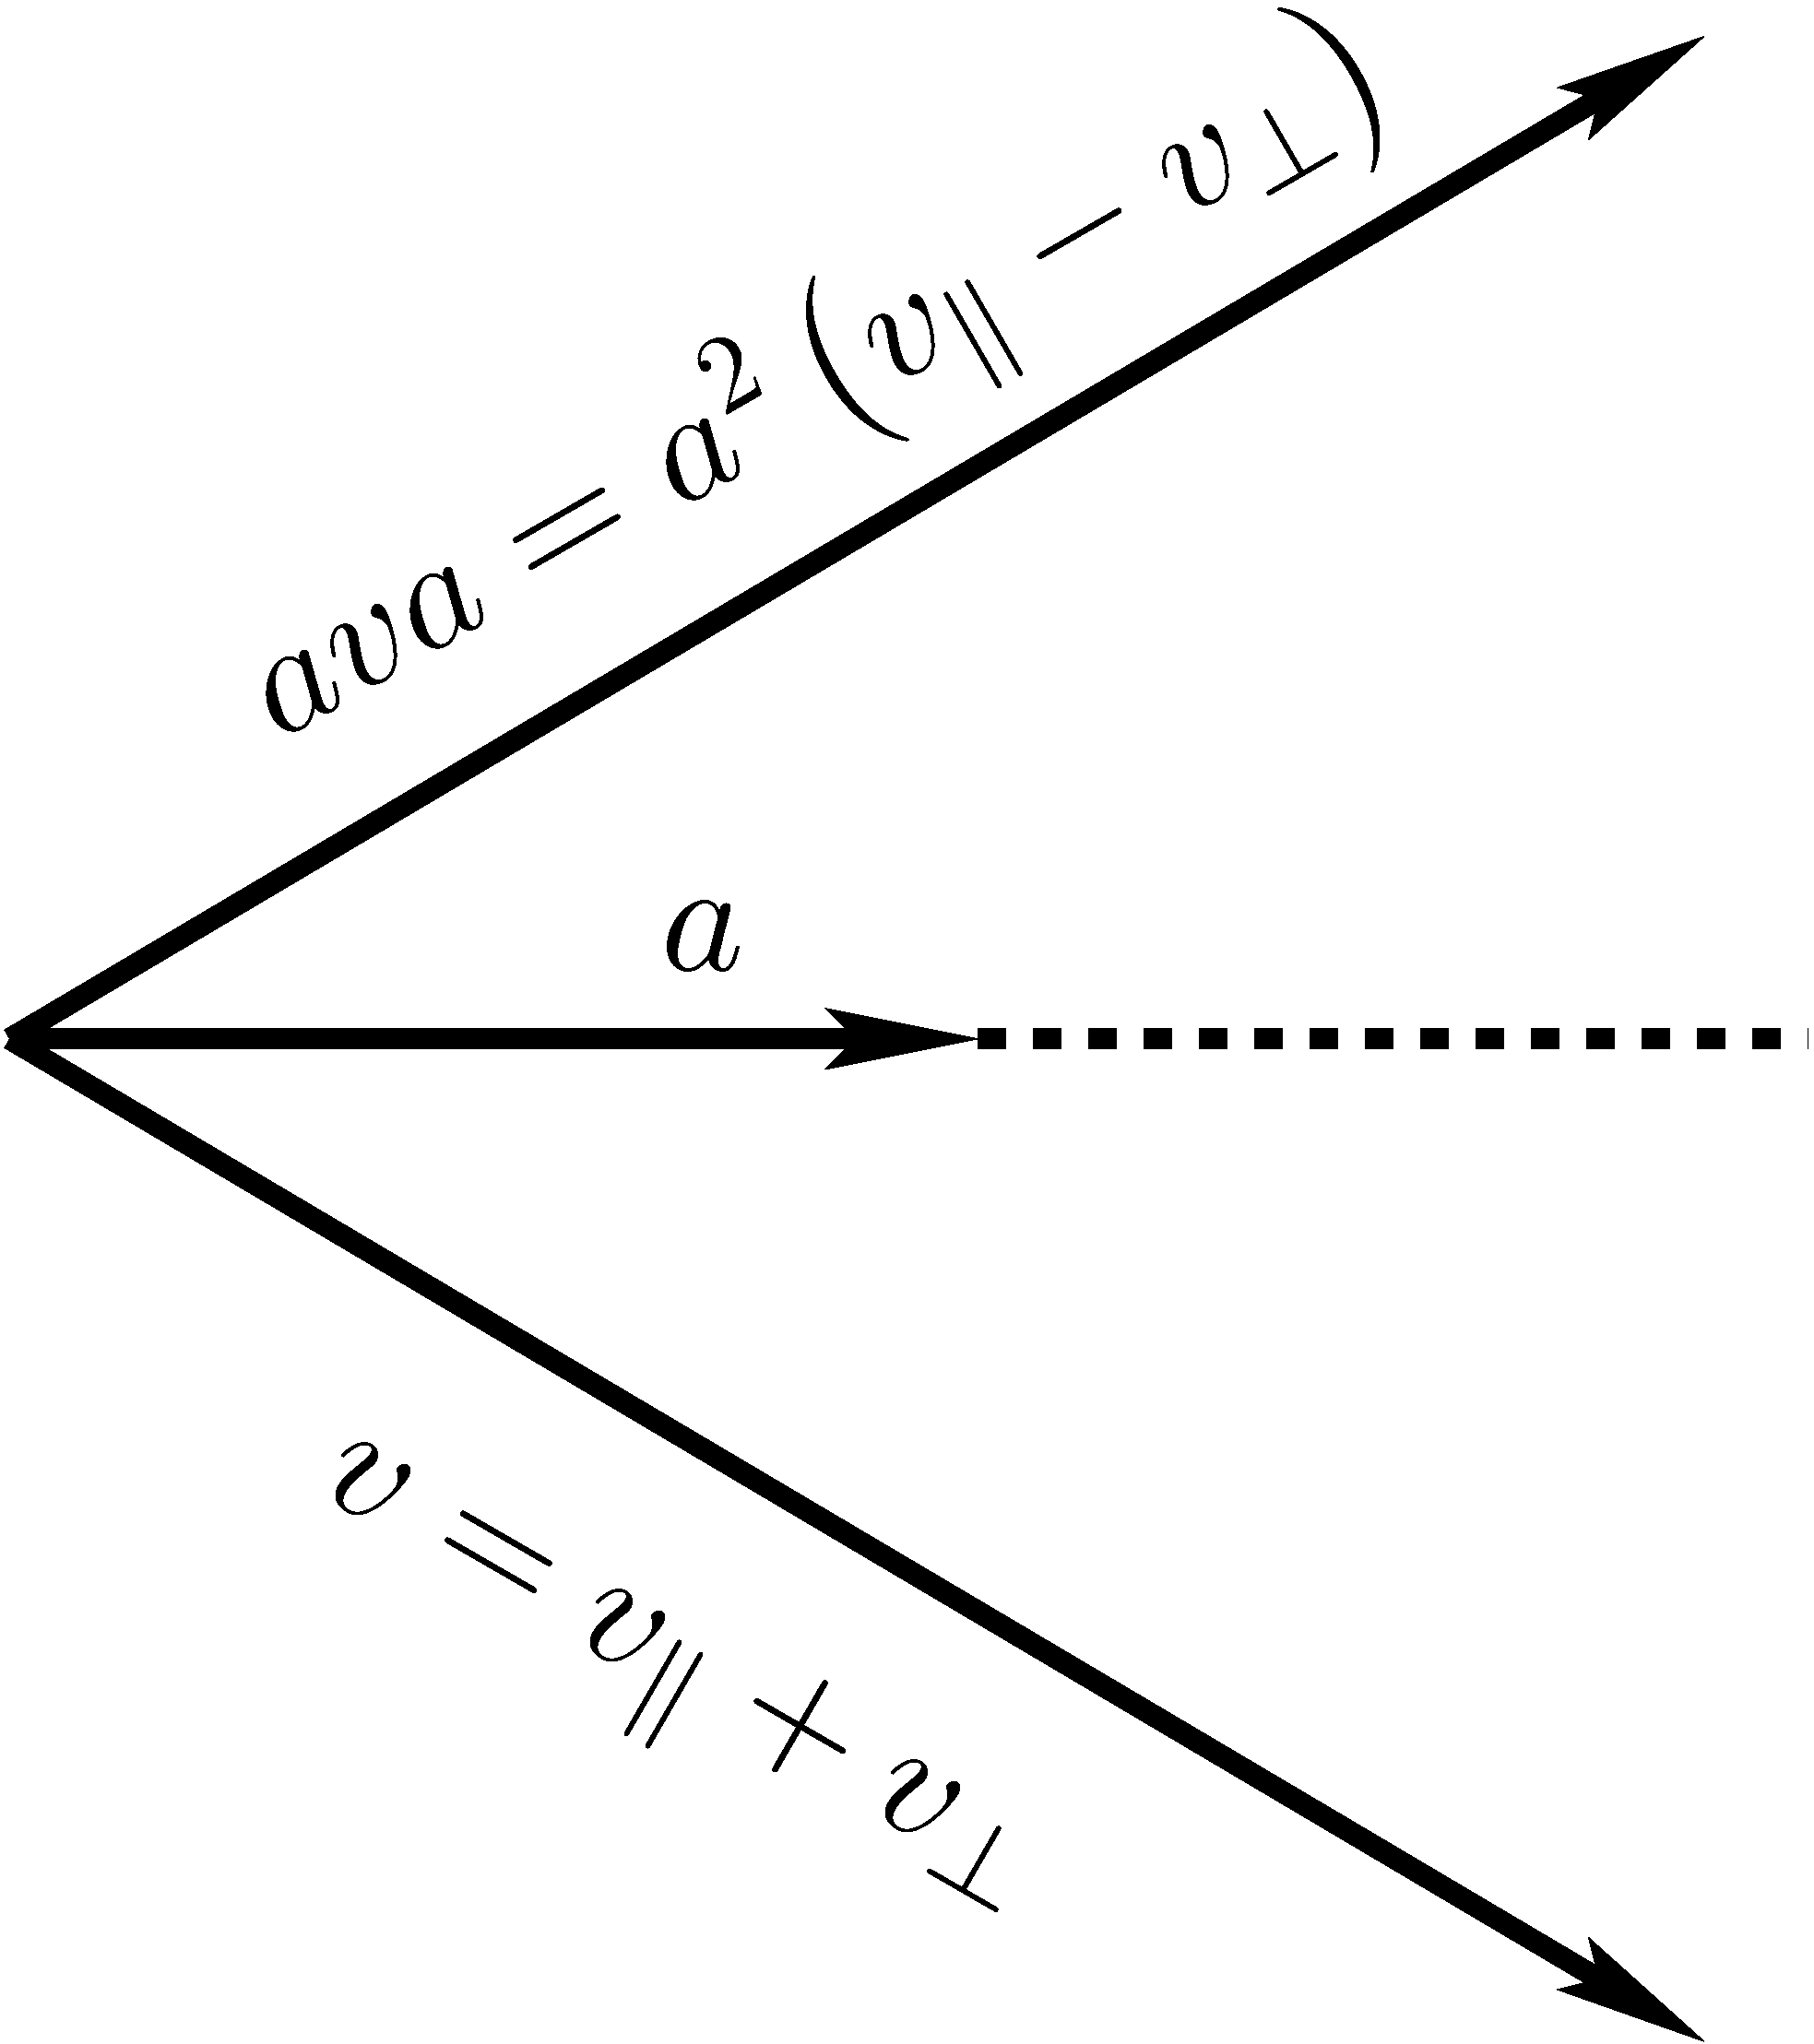
\includegraphics{reflect.png}}
\caption{Reflection of Vector}
\end{center}
\end{figure}
\begin{enumerate}
\item Decompose $v = v_{\parallel}+v_{\perp}$ where $v_{\parallel}$ is the part of $v$
parallel to $a$ and $v_{\perp}$ is the part perpendicular to $a$.
\item $av = av_{\parallel}+av_{\perp} = v_{\parallel}a-v_{\perp}a$ since $a$ and $v_{\perp}$ are
orthogonal.
\item $ava = a^{2}\lp v_{\parallel}-v_{\perp}\rp$ is a vector since $a^{2}$ is a scalar.
\item $ava$ is the reflection of $v$ about the direction of $a$ if $a^{2} = 1$.
\item Thus $\vprod{a_{1}}{a_{r}}v\vprod{a_{r}}{a_{1}} \in \Vsp$ and produces a composition of reflections
of $v$ if $a^{2}_{1} = \dots = a^{2}_{r} = 1$.
\end{enumerate}

\section{Rotations}\label{sec1_10}
\subsection{Definitions}
First define the reverse of a product of vectors. If $R = \vprod{a_{1}}{a_{s}}$ then the reverse is
$R^{\R} = \lp\vprod{a_{1}}{a_{s}}\rp^{\R} = \vprod{a_{r}}{a_{1}}$, the order of multiplication
is reversed. Then let $R = ab$ so that
\be
RR^{\R} = (ab)(ba) = ab^{2}a = a^{2}b^{2} = R^{\R}R
\ee
Let $RR^{\R} = 1$ and calculate $\lp RvR^{\R}\rp^{2}$, where $v$ is an arbitrary vector.
\be
     \lp RvR^{\R}\rp^{2} = RvR^{\R}RvR^{\R} = Rv^{2}R^{\R} = v^{2}RR^{\R} = v^{2}
\ee
Thus $RvR^{\R}$ leaves the length of $v$ unchanged. Now we must also prove $Rv_{1}R^{\R}\cdot R v_{2}R^{\R} = v_{1}\cdot v_{2}$. Since
$Rv_{1}R^{\R}$ and $Rv_{2}R^{\R}$ are both vectors we can use the definition of the
dot product for two vectors
\begin{align*}
Rv_{1}R^{\R}\cdot R v_{2}R^{\R} & = \half\lp Rv_{1}R^{\R}Rv_{2}R^{\R}+Rv_{2}R^{\R}Rv_{1}R^{\R} \rp \\
                              & = \half\lp Rv_{1}v_{2}R^{\R}+Rv_{2}v_{1}R^{\R} \rp  \\
                              & = \half R\lp v_{1}v_{2}+v_{2}v_{1}\rp R^{\R} \\
                              & = R\lp v_{1}\cdot v_{2}\rp R^{\R} \\
                              & = v_{1}\cdot v_{2}RR^{\R} \\
                              & = v_{1}\cdot v_{2}
\end{align*}
Thus the transformation $RvR^{\R}$ preserves both length and angle and must be a rotation. The normal 
designation for $R$ is a rotor.  If we have a series of successive rotations $R_{1},R_{2},\dots,R_{k}$ to be applied to a vector $v$ then
the result of the $k$ rotations will be
$$
	R_{k}R_{k-1}\dots R_{1}vR_{1}^{\R}R_{2}^{\R}\dots R_{k}^{\R}
$$
Since each individual rotation can be written as the geometric product of two vectors, the composition of 
$k$ rotations can be written as the geometric product of $2k$ vectors.  The multivector that results from
the geometric product of $r$ vectors is called a {\bf versor} of order $r$. A composition of rotations is
always a versor of even order.
\subsection{General Rotation}\label{sec1_10_2}
The general rotation can be represented by $R = e^{\thh u}$ where $u$ is a unit
bivector in the plane of the rotation and $\theta$ is the rotation angle in 
the plane.\footnote{$e^{A}$ is defined as the 
Taylor series expansion $e^{A} = {\ds\sum_{j=0}^{\infty}\frac{A^{j}}{j!}}$ where $A$ is any multivector.}
 The two possible non-degenerate cases are $u^{2} = \pm 1$
\be
e^{\thh u} = \left \{
\begin{array}{crl}
\mbox{(Euclidean plane)} & u^{2} = -1: & \cosf{\thh}+u\sinf{\thh} \\
\mbox{(Minkowski plane)} & u^{2} = 1:  & \coshf{\thh}+u\sinhf{\thh} \\
\end{array}
\right \}
\ee
Decompose $v = \vp+\lp v-\vp \rp$ where $\vp$ is the projection of $v$ into the plane defined 
by $u$. Note that $v-\vp$ is orthogonal to all vectors in the $u$ plane. Now let $u = \epep$ where $\epar$ is
parallel to $\vp$ and of course $\eperp$ is in the plane $u$ and orthogonal to $\epar$. $v-\vp$ anticommutes with
$\epar$ and $\eperp$ and $\vp$ anticommutes with $\eperp$ (it is left to the reader to show $RR^{\R} = 1$).

\subsection{Euclidean Case}
For the case of $u^{2} = -1$
\begin{figure}[htbp]
\begin{center}
\scalebox{0.65}{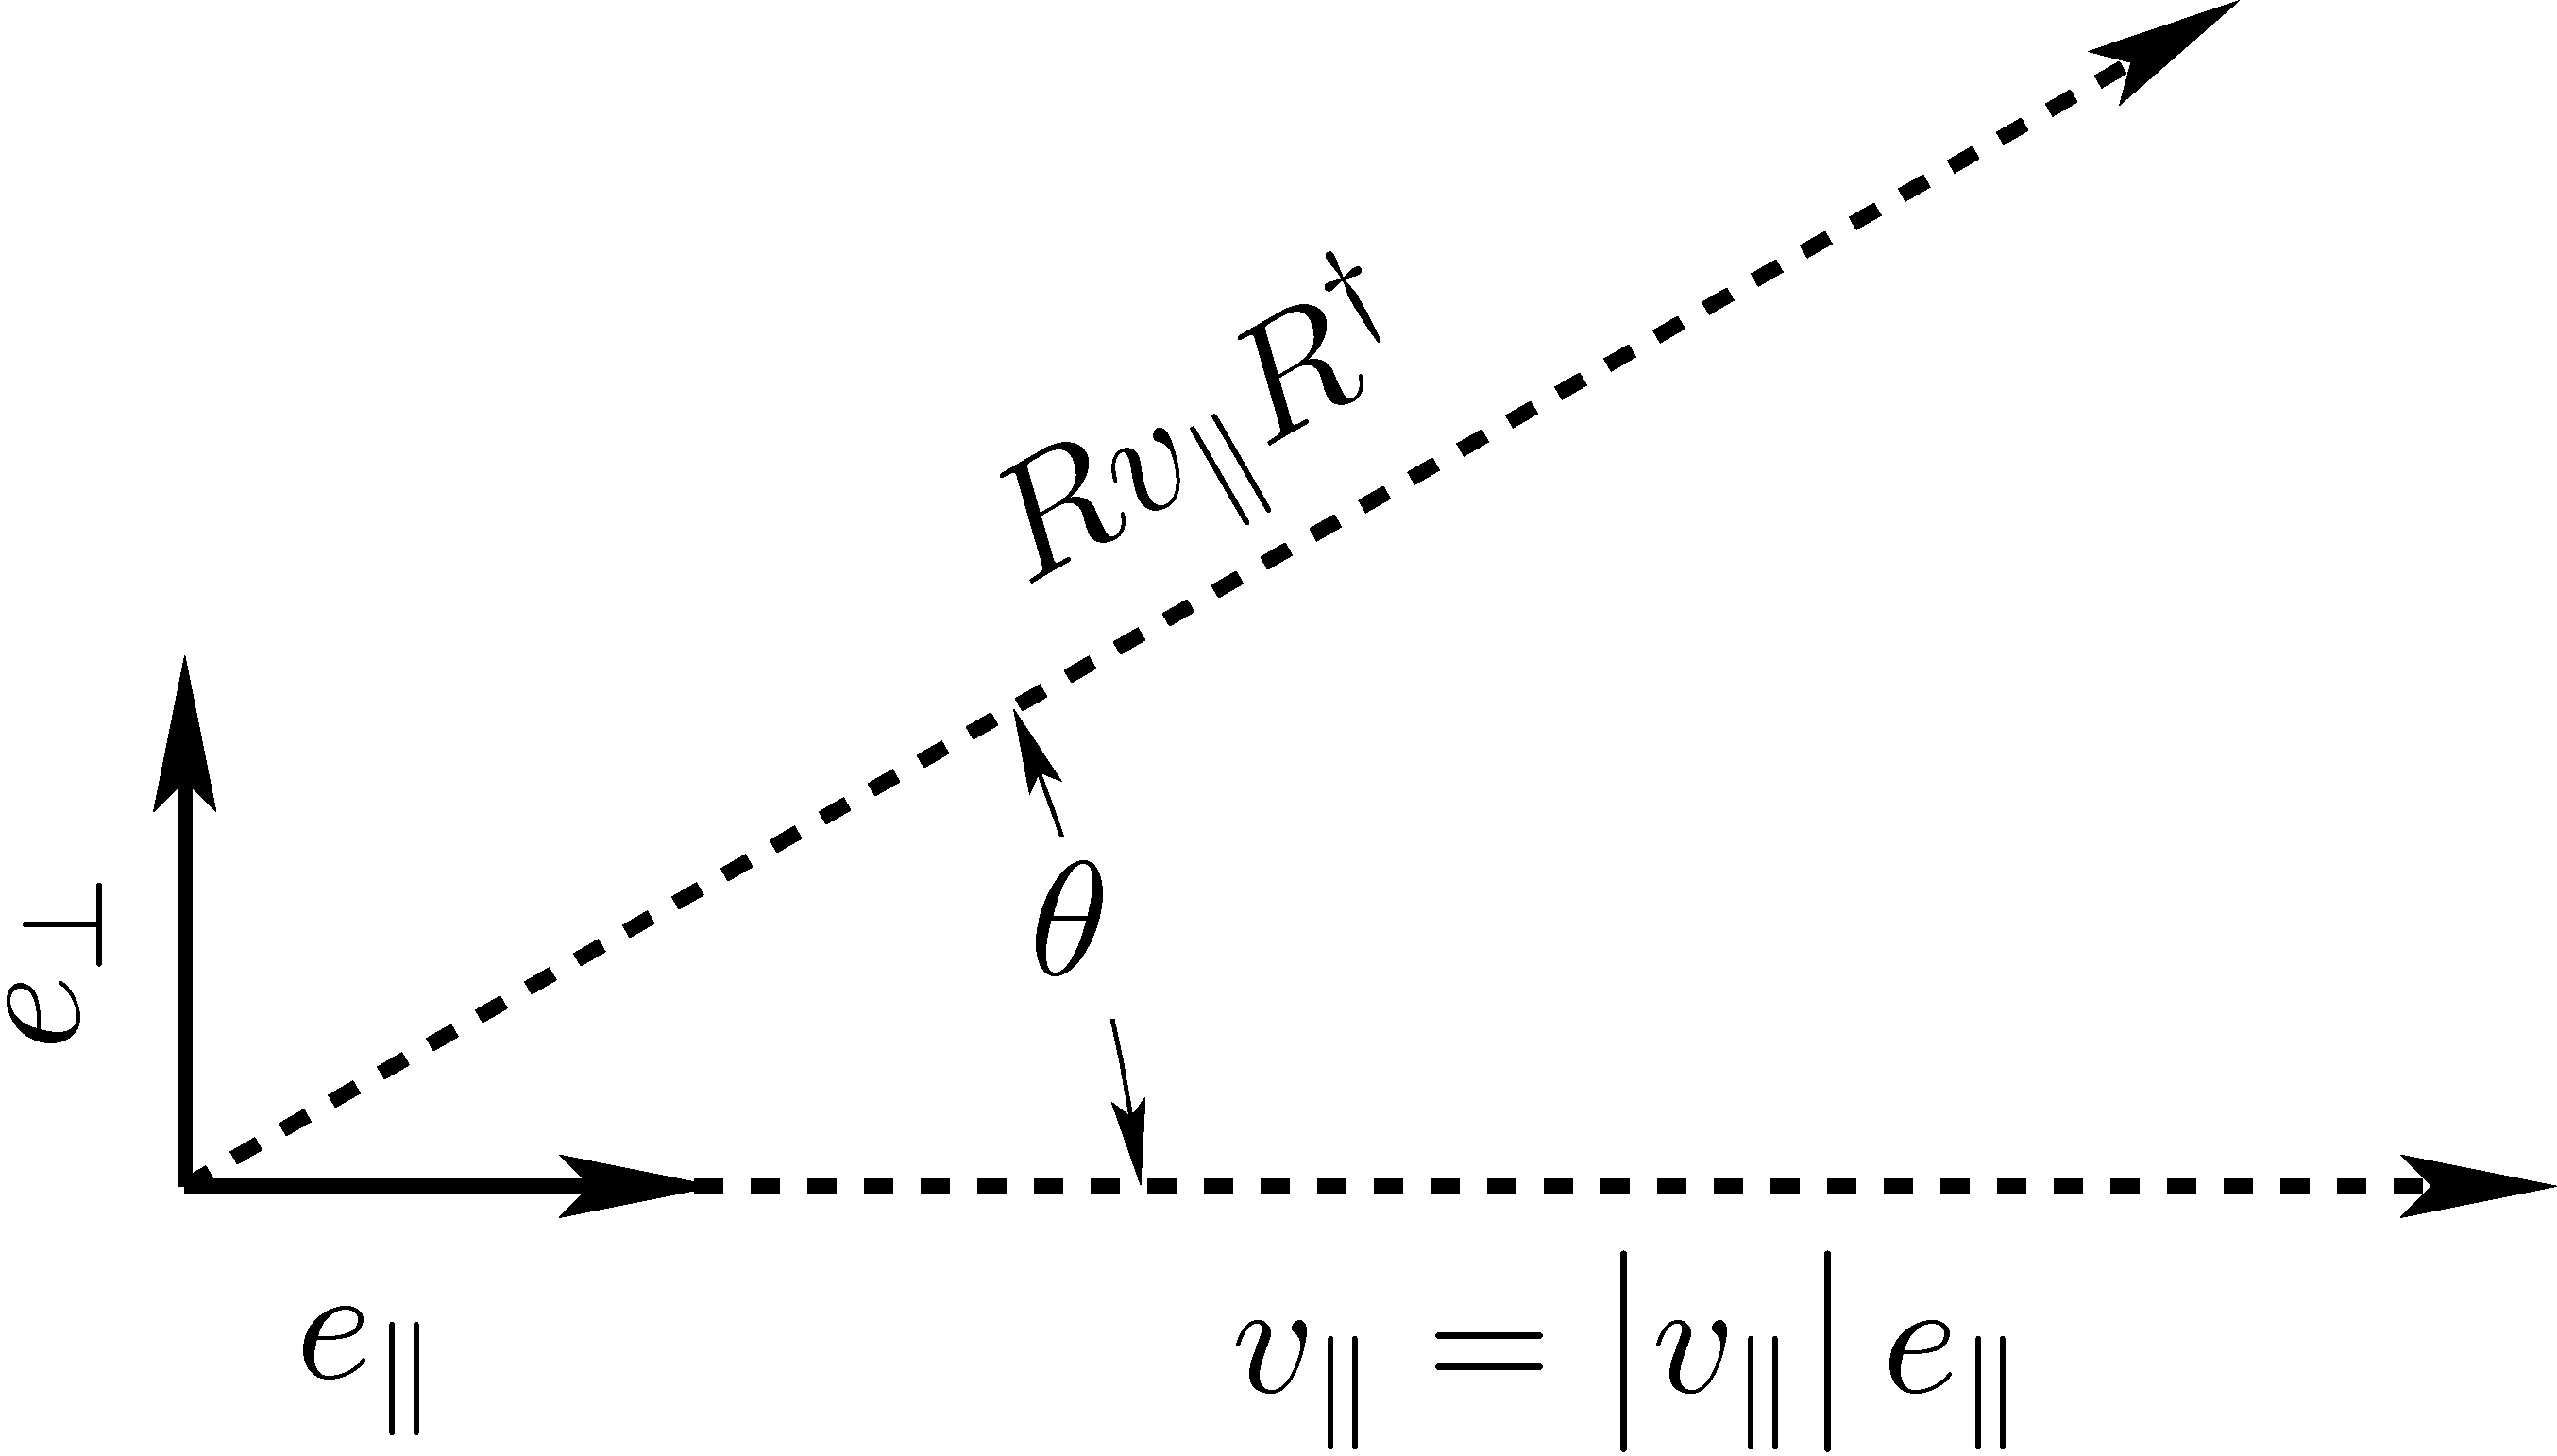
\includegraphics{rotate.png}}
\caption{Rotation of Vector}
\end{center}
\end{figure}

$$
\hspace{-0.5in}RvR^{\R} = \lp \cosf{\thh}+\epep\sinf{\thh}\rp\lp \vp+\lp v-\vp \rp \rp \lp\cosf{\thh}+\epepr\sinf{\thh}\rp
$$

Since $v-\vp$ anticommutes with $\epar$ and $\eperp$ it commutes with $R$ and 
\be
RvR^{\R} = R\vp R^{\R} +\lp v-\vp \rp
\ee
So that we only have to evaluate
\be
\hspace{-0.5in}R\vp R^{\R} =  \lp \cosf{\thh}+\epep\sinf{\thh}\rp\vp\lp\cosf{\thh}+\epepr\sinf{\thh}\rp
\ee
Since $\vp = \abs{\vp}\epar$
\be
R\vp R^{\R} = \abs{\vp}\lp \cosf{\theta}\epar+\sinf{\theta}\eperp \rp
\ee
and the component of $v$ in the $u$ plane is rotated correctly.

\subsection{Minkowski Case}
For the case of $u^{2} = 1$ there are two possibilities, $\vp^{2} > 0$ or $\vp^{2} < 0$.
In the first case $\epar^{2} = 1$ and $\eperp^{2} = -1$. In the second case $\epar^{2} = -1$ 
and $\eperp^{2} = 1$. Again $v-\vp$ is not affected by the rotation so that we need only
evaluate
$$
R\vp R^{\R} =\lp \coshf{\thh}+\epep\sinhf{\thh}\rp\vp\lp\coshf{\thh}+\epepr\sinhf{\thh}\rp
$$
Note that in this case $\abs{\vp} = \sqrt{\abs{\vp^{2}}}$ and
\be
R\vp R^{\R} = \left \{
\begin{array}{c}
\vp^{2} > 0: \abs{\vp}\lp\coshf{\theta}\epar+\sinhf{\theta}\eperp \rp  \\
\vp^{2} < 0: \abs{\vp}\lp\coshf{\theta}\epar-\sinhf{\theta}\eperp \rp  \\
\end{array}
\right \}
\ee
\section{Expansion of geometric product and generalization of $\cdot$ and $\w$}
If $A_{r}$ and $B_{s}$ are respectively grade $r$ and $s$ pure grade multivectors
then
\be\label{21}
\hspace{-0.25in}A_{r}B_{s} = \proj{A_{r}B_{s}}{\abs{r-s}}+\proj{A_{r}B_{s}}{\abs{r-s}+2}+\cdots+
             \proj{A_{r}B_{s}}{\min(r+s,2N-(r+s))}
\ee
\be\label{22}
A_{r}\cdot B_{s} \equiv \proj{A_{r}B_{s}}{\abs{r-s}}
\ee
\be\label{23}
A_{r}\w B_{s} \equiv \proj{A_{r}B_{s}}{r+s}
\ee
Thus if $r+s > N$ then $A_{r}\w B_{s} = 0$, also note that these formulas are the most efficient
way of calculating $A_{r}\cdot B_{s}$ and $A_{r}\w B_{s}$.  Using equations~\ref{17} and \ref{21} we 
can prove that for a vector $a$ and a grade $r$ multivector $B_{r}$
\be\label{24}
     a\cdot B_{r} = \half\paren{aB_{r}-\paren{-1}^{r}B_{r}a}
\ee
\be\label{25}
     a\w B_{r} = \half\paren{aB_{r}+\paren{-1}^{r}B_{r}a}
\ee
If equations~\ref{24} and \ref{25} are true for a grade $r$ blade they are also true for a grade $r$
multivector (superposition of grade $r$ blades). By equation~\ref{17} let 
$B_{r} = \vprod{e_{1}}{e_{r}}$ where the $e's$ are orthogonal and expand $a$ 
\be
a = a_{\perp}+\sum^{r}_{j=1}\alpha_{j}e_{j}
\ee
where $a_{\perp}$ is orthogonal to all the $e's$.
Then\footnote{$e_{1}\dots e_{j-1}\breve{e}_{j}e_{j+1}\dots e_{r} 
= e_{1}\dots e_{j-1}e_{j+1}\dots e_{r}$}
\begin{align}\label{27}
aB_{r} & = \sum^{r}_{j=1}(-1)^{j-1}\alpha_{j}e_{j}^{2}e_{1}\cdots \breve{e}_{j}\cdots e_{r}
              +a_{\perp}\vprod{e_{1}}{e_{r}} \nonumber \\
       & = a\cdot B_{r} + a\w B_{r}
\end{align}
Now calculate
\begin{align}\label{30}
B_{r}a & = \sum^{r}_{j=1}(-1)^{r-j}\alpha_{j}e_{j}^{2}e_{1}\cdots \breve{e}_{j}\cdots e_{r}
           -\paren{-1}^{r-1}a_{\perp}\vprod{e_{1}}{e_{r}} \nonumber \\
       & = \paren{-1}^{r-1}\paren{\sum^{r}_{j=1}(-1)^{j-1}\alpha_{j}e_{j}^{2}e_{1}\cdots \breve{e}_{j}\cdots e_{r}
           -a_{\perp}\vprod{e_{1}}{e_{r}}} \nonumber \\
       & = \paren{-1}^{r-1}\paren{a\cdot B_{r}-a\w B_{r}} 
\end{align}
Adding and subtracting equations~\ref{27} and \ref{30} gives equations~\ref{24} and \ref{25}.
\section{Duality and the Pseudoscalar}
If $e_{1},\dots,e_{n}$ is an orthonormal basis for the vector space the the pseudoscalar $I$ is defined by
\be\label{40}
	I = \vprod{e_{1}}{e_{n}}
\ee
Since one can transform one orthonormal basis to another by an orthogonal transformation the $I$'s for all
orthonormal bases are equal to within a $\pm 1$ scale factor with depends on the ordering of the basis vectors.
If $A_{r}$ is a pure $r$ grade multivector $\paren{A_{r} = \proj{A_{r}}{r}}$ then
\be\label{41}
	A_{r}I = \proj{A_{r}I}{n-r}
\ee
or $A_{r}I$ is a pure $n-r$ grade multivector.  Further by the symmetry properties of $I$ we have
\be\label{42}
	IA_{r} = \paren{-1}^{\paren{n-1}r}A_{r}I
\ee
$I$ can also be used to exchange the $\cdot$ and $\w$ products as follows using equations~\ref{24} and
\ref{25}
\begin{align}
	a\cdot\paren{A_{r}I} & =  \half\paren{aA_{r}I-\paren{-1}^{n-r}A_{r}Ia} \\
						 & =  \half\paren{aA_{r}I-\paren{-1}^{n-r}\paren{-1}^{n-1}A_{r}aI} \\
                         & =  \half\paren{aA_{r}+\paren{-1}^{r}A_{r}a}I \\
						 & = \paren{a\w A_{r}}I \label{25a}
\end{align}

More generally if $A_{r}$ and $B_{s}$ are pure grade multivectors with $r+s \le n$ we have using
equation~\ref{22} and \ref{41}
\begin{align}
	A_{r}\cdot\paren{B_{s}I} & = \proj{A_{r}B_{s}I}{\abs{r-\paren{n-s}}} \\
							 & = \proj{A_{r}B_{s}I}{n-\paren{r+s}} \\
							 & = \proj{A_{r}B_{s}}{r+s}I \\
							 & = \paren{A_{r}\w B_{s}}I
\end{align}
Finally we can relate $I$ to $I^{\R}$ by
\be
	I^{\R} = \paren{-1}^{\frac{n\paren{n-1}}{2}}I
\ee
\section{Reciprocal Frames}
Let $\lst{\eb_{1}}{\eb_{n}}$ be a set of linearly independent vectors that span the vector space that are
not necessarily orthogonal. These vectors define the frame (frame vectors are shown in bold face since they are almost always associated with a particular coordinate system) with volume element
\be
	E_{n} \equiv \wprod{\eb_{1}}{\eb_{n}}
\ee
So that $E_{n} \propto I$.  The reciprocal frame is the set of vectors $\lst{\eb^{1}}{\eb^{n}}$ that satisfy the relation
\be
	\eb^{i}\cdot \eb_{j} = \delta^{i}_{j},\quad \forall i,j = 1,\dots,n
\ee
The $\eb^{i}$ are constructed as follows
\be\label{eq61}
	\eb^{j} = \paren{-1}^{j-1}\eb_{1}\w\eb_{2}\w\dots\w\breve{\eb}_{j}\w\dots\w\eb_{n}E_{n}^{-1}
\ee
So that the dot product is (using equation~\ref{25a} since $E_{n}^{-1} \propto I$)
\begin{align}
	\eb_{i}\cdot\eb^{j} &= \paren{-1}^{j-1}\eb_{i}\cdot\paren{\eb_{1}\w\eb_{2}\w\dots\w\breve{\eb}_{j}
							\w\dots\w\eb_{n}E_{n}^{-1}} \\
 						&= \paren{-1}^{j-1}\paren{\eb_{i}\w\eb_{1}\w\eb_{2}\w\dots\w\breve{\eb}_{j}
							\w\dots\w\eb_{n}}E_{n}^{-1} \\
						&= 0,\quad\forall i \ne j
\end{align}
and
\begin{align}
	\eb_{1}\cdot\eb^{1} & = \eb_{1}\cdot\paren{\wprod{\eb_{2}}{\eb_{n}}E_{n}^{-1}} \\
						& = \paren{\eb_{1}\w\wprod{\eb_{2}}{\eb_{n}}}E_{n}^{-1} \\
						& = 1 
\end{align}
\section{Coordinates}
The reciprocal frame can be used to develop a coordinate representation for multivectors in an arbitrary frame
$\eb_{1},\dots,\eb_{n}$ with reciprocal frame $\eb^{1},\dots,\eb^{n}$.
Since both the frame and it's reciprocal span the base vector space we can write any vector $a$ in the vector space
as
\be
	a = a^{i}\eb_{i} = a_{i}\eb^{i}
\ee
where if an index such as $i$ is repeated it is assumes that the terms with the repeated index will be summed from
$1$ to $n$. Using that $\eb_{i}\cdot\eb^{j} = \delta_{i}^{j}$ we have
\begin{align}
	a_{i} &= a\cdot\eb_{i} \\
	a^{i} &= a\cdot\eb^{i}
\end{align}
In tensor notation $a_{i}$ would be the covariant representation and $a^{i}$ the contravariant representation of the 
vector $a$.  Now consider the case of grade 2 and grade 3 blades:
\begin{align}
	\eb^{i}\cdot\paren{a\w b} &= a\cdot\eb^{i}b-b\cdot\eb^{i}a \nonumber \\
	\eb_{i}\paren{a\cdot\eb^{i}b-b\cdot\eb^{i}a} &= ab-ba = 2a\w b \nonumber \\
	\eb^{i}\cdot\paren{a\w b\w c} &= a\cdot\eb^{i}b\w c-b\cdot\eb^{i}a\w c+ c\cdot\eb^{i}a\w b \nonumber \\
	\eb_{i}\paren{a\cdot\eb^{i}b\w c-b\cdot\eb^{i}a\w c+ c\cdot\eb^{i}a\w b} &= ab\w c-ba\w c+ca\w b = 3a\w b\w c \nonumber 
\end{align}
for an $r$-blade $A_{r}$ we have (the proof is left to the reader)
\be\label{eq71}
	\eb_{i}\eb^{i}\cdot A_{r} = rA_{r}
\ee
Since $\eb_{i}\eb^{i} = n$ we have
\be\label{eq72}
	\eb_{i}\eb^{i}\w A_{r} = \eb_{i}\paren{\eb^{i}A_{r}-\eb^{i}\cdot A_{r}} = \paren{n-r}A_{r}
\ee
Flipping $\eb^{i}$ and $A_{r}$ in equations~\ref{eq71} and \ref{eq72} and subtracting equation~\ref{eq71}
from \ref{eq72} gives
\be
	\eb_{i}A_{r}\eb^{i} = \paren{-1}^{r}\paren{n-2r}A_{r}
\ee
In Hestenes and Sobczyk (3.14) it is proved that
\be
	\paren{\eb^{k_{r}}\w\dots\w\eb^{k_{1}}}\cdot\paren{\eb_{j_{1}}\w\dots\w\eb_{j_{r}}} =
	\delta_{k_{1}}^{j_{1}}\delta_{k_{2}}^{j_{2}}\dots\delta_{k_{r}}^{j_{r}}
\ee
so that the general multivector $A$ can be expanded in terms of the blades of the frame and reciprocal frame as
\be\label{eq1_75}
	A = \sum_{i<j<\cdots<k} A_{ij\cdots k}\eb^{i}\w\eb^{j}\w\cdots\w\eb^{k}
\ee
where
\be\label{eq1_76}
	A_{ij\cdots k} = \paren{\eb_{k}\w\cdots\w\eb_{j}\w\eb_{i}}\cdot A
\ee
The components $A_{ij\cdots k}$ are totally antisymmetric on all indices and are usually referred to
as the components of an {\em antisymmetric tensor}.
\section{Linear Transformations}\label{sec1_15}
\subsection{Definitions}
Let $f$ be a linear transformation on a vector space $f:\Vsp \rightarrow \Vsp$ with 
$\fof{f}{\alpha a+\beta b} = \alpha\fof{f}{a}+\beta\fof{f}{b}$ $\forall a,b \in \Vsp$
and $\alpha,\beta \in \Re$. Then define the action of $f$ on a blade of the geometric
algebra by
\be\label{eq1_77}
\fof{f}{\wprod{a_{1}}{a_{r}}} = \wprod{\fof{f}{a_{1}}}{\fof{f}{a_{1}}}
\ee
and the action of $f$ on any two $A,B \in \GA{\Vsp}$ by
\be
\fof{f}{\alpha A + \beta B} = \alpha\fof{f}{A}+\beta\fof{f}{B}
\ee
Since any multivector $A$ can be expanded as a sum of blades $\fof{f}{A}$ is
defined. This has many consequences. Consider the following definition for the determinant
of $f$, $\fof{\det}{f}$.
\be\label{1_79}
\fof{f}{I} = \fof{\det}{f}I
\ee
First show that this definition is equivalent to the standard definition of the 
determinant (again $\mset{e_{1}}{e_{N}}$ is an orthonormal basis for $\Vsp$).
\be
\fof{f}{e_{r}} = \sum_{s = 1}^{N}a_{rs}e_{s}
\ee
Then
\begin{align}
\fof{f}{I} &= \wprod{\paren{\sum_{s_{1} = 1}^{N}a_{1s_{1}}e_{s}}}
              {\paren{\sum_{s_{N} = 1}^{N}a_{Ns_{N}}e_{s}}} \nonumber \\
           &= \sum_{\mset{s_{1}}{s_{N}}} \vprod{a_{1s_{1}}}{a_{Ns_{N}}}\vprod{e_{s_{1}}}{e_{s_{N}}}
\end{align}
But
\be
\vprod{e_{s_{1}}}{e_{s_{N}}} = \varepsilon_{\vprod{1}{N}}^{\vprod{s_{1}}{s_{N}}}\vprod{e_{1}}{e_{N}}
\ee
so that
\be
\fof{f}{I} = \sum_{\mset{s_{1}}{s_{N}}} \varepsilon_{\vprod{1}{N}}^{\vprod{s_{1}}{s_{N}}}
             \vprod{a_{1s_{1}}}{a_{Ns_{N}}}I
\ee
or
\be
\fof{\det}{f} = \sum_{\mset{s_{1}}{s_{N}}} \varepsilon_{\vprod{1}{N}}^{\vprod{s_{1}}{s_{N}}}
             \vprod{a_{1s_{1}}}{a_{Ns_{N}}}
\ee
which is the standard definition. Now compute the determinant of the product of the linear
transformations $f$ and $g$
\begin{align}
\fof{\det}{fg}I &= \fof{fg}{I} \nonumber \\
               &= \fof{f}{\fof{g}{I}} \nonumber \\
               &= \fof{f}{\fof{\det}{g}I} \nonumber \\
               &= \fof{\det}{g}\fof{f}{I} \nonumber \\
               &= \fof{\det}{g}\fof{\det}{f}I 
\end{align}
or
\be
\fof{\det}{fg} = \fof{\det}{f}\fof{\det}{g}
\ee
Do you have any idea of how miserable that is to prove from the standard definition of determinant?
\subsection{Adjoint}
If $F$ is linear transformation and $a$ and $b$ are two arbitrary vectors the adjoint function, $\adj{F}$, is
defined by
\be
	a\cdot \adjf{F}{b} = b\cdot F\paren{a}
\ee
From the definition the adjoint is also a linear transformation. For an arbitrary frame $\eb_{1},\dots,\eb_{n}$
we have
\be
	\eb_{i}\cdot \adjf{F}{a} = a\cdot F\paren{\eb_{i}}
\ee
So that we can explicitly construct the adjoint as
\begin{align}
	\adjf{F}{a} & = \eb^{i}\paren{\eb_{i}\cdot \adjf{F}{a}} \nonumber \\
	            & = \eb^{i}\paren{a\cdot \f{F}{\eb_{i}}} \nonumber \\
		        & = \eb^{i}\paren{\f{F}{\eb_{i}}\cdot\eb^{j}}a_{j}
\end{align}
so that $\adj{F}_{ij} = F\paren{\eb_{i}}\cdot\eb^{j}$ is the matrix representation of $\adj{F}$ for the 
$\eb_{1},\dots,\eb_{n}$ frame. However
\be
	F\paren{a} = \eb^{i}\paren{F\paren{\eb^{j}}\cdot\eb_{i}}a_{j}
\ee
so that the matrix representation of $F$ is $F_{ij} = F\paren{\eb^{j}}\cdot\eb_{i}$. If the $\eb_{1},\dots,\eb_{n}$ are
orthonormal then $\eb_{j} = \eb^{j}$ for all $j$ and $\adj{F}_{ij} = F_{ji}$ exactly the same as the adjoint in matrices.

Other basic properties of the adjoint are:
\be
	\adj{\adj{F}}\paren{a} = \eb^{i}a\cdot\adjf{F}{\eb_{i}} = \eb^{i}\eb_{i}\cdot F\paren{a} = F\paren{a}
\ee
and
\begin{align}
	\adjf{FG}{a} & = \eb^{i}\lp \eb_{i}\cdot\adjf{FG}{a} \rp \nonumber \\
			     & = \eb^{i}\lp a\cdot\f{F}{\f{G}{\eb_{i}}} \rp \nonumber \\
			     &=  \eb^{i}\lp \adjf{F}{a}\cdot\f{G}{\eb_{i}} \rp \nonumber \\
			     &=  \eb^{i}\lp \eb_{i}\cdot\adjf{G}{\adjf{F}{a}} \rp \nonumber \\
			     &=  \adjf{G}{\adjf{F}{a}} 
\end{align}
so that $\adj{\adj{F}} = F$ and $\adj{FG} = \adj{G}\,\adj{F}$.
A symmetric function is one where $F = \adj{F}$.  As an
example consider $F\adj{F}$
\be
	\adj{F\adj{F}} = \adj{\adj{F}}\,\adj{F} = F\adj{F}
\ee
\subsection{Inverse}
Another linear algebraic relation in geometric algebra is
\be
f^{-1}\paren{A} = \bfrac{I\adjf{f}{I^{-1}A}}{\det\paren{f}}\ \  \forall A \in \GA{\Vsp}\label{eq1_94}
\ee
where $\adj{f}$ is the adjoint transformation defined by $a\cdot\adjf{f}{b} = b\cdot\fof{f}{a}$
 $\forall a,b \in \Vsp$ and you have an explicit formula for the inverse of a linear transformation!
\section{Commutator Product}\label{sec1_16}
The commutator product of two multivectors $A$ and $B$ is defined as
\be
	A\cross B \equiv \half\paren{AB-BA}
\ee
An important theorem for the commutator product is that for a grade 2 multivector, $A_{2} = \proj{A}{2}$,
and a grade $r$ multivector $B_{r} = \proj{B}{r}$ we have
\be\label{eq131}
 A_{2}B_{r} = A_{2}\w B_{r}+A_{2}\cross B_{r}+A_{2}\cdot B_{r}
\ee
From the geometric product grade expansion for multivectors we have
\be
 A_{2}B_{r} = \proj{A_{2}B_{r}}{r+2}+\proj{A_{2}B_{r}}{r}+\proj{A_{2}B_{r}}{\abs{r-2}}	
\ee 
Thus we must show that 
\be
	\proj{A_{2}B_{r}}{r} = A_{2}\cross B_{r}
\ee
Let $e_{1},\dots,e_{n}$ be an orthogonal set for the vector space where $B_{r} = e_{1}\dots e_{r}$ and 
$A_{2} = {\ds \sum_{l<m=2}^{n}\alpha_{lm}e_{l}e_{m}}$ so we can write
\be
A_{2}\cross B_{r} = \paren{\sum_{l<m=2}^{n}\alpha_{lm}e_{l}e_{m}}\cross\paren{e_{1}\dots e_{r}}
\ee 
Now consider the following three cases
\begin{enumerate}
\item $l \mbox{ and } m > r$ where $e_{l}e_{m}e_{1}\dots e_{r} = e_{1}\dots e_{r}e_{l}e_{m}$
\item $l \le r \mbox{ and } m > r$ where $e_{l}e_{m}e_{1}\dots e_{r} = -e_{1}\dots e_{r}e_{l}e_{m}$
\item $l \mbox{ and } m \le r$ where $e_{l}e_{m}e_{1}\dots e_{r} = e_{1}\dots e_{r}e_{l}e_{m}$
\end{enumerate}
For case~1 and 3 $e_{l}e_{m}$ commute with $B_{r}$ and the contribution to the commutator product is zero.  In
case~3 $e_{l}e_{m}$ anticommutes with $B_{r}$ and thus are the only terms that contribute to the commutator.  All
these terms are of grade $r$ and the theorem is proved.  Additionally, the commutator product obeys the Jacobi identity
\be\label{jacobi}
	A\cross\paren{B\cross C} = \paren{A\cross B}\cross C+B\cross\paren{A\cross C}	
\ee
This is important for the geometric algebra treatment of Lie groups and algebras.

\chapter{Examples of Geometric Algebra}
\section{Quaternions}
Any multivector $A \in \GA{3,0}$ may be written as
\be
A = \alpha + a + B + \beta I
\ee 
where $\alpha,\beta \in \Re$, $a \in \Vsp\lp 3,0 \rp$, $B$ is a bivector, and
$I$ is the unit pseudoscalar. The quaternions are the multivectors of even grades
\be
A = \alpha + B
\ee
$B$ can be represented as
\be
B = \alpha{\bf i}+\beta{\bf j} + \gamma{\bf k}
\ee
where ${\bf i} = e_{2}e_{3}$, ${\bf j} = e_{1}e_{3}$, and ${\bf k} = e_{1}e_{2}$, and
\be
{\bf i}^{2} = {\bf j}^{2} = {\bf k}^{2} = {\bf ijk} = -1.
\ee
The quaternions form a subalgebra of $\GA{3,0}$ since the geometric product of any
two quaternions is also a quaternion since the geometric product of two even grade
multivector components is a even grade multivector. For example the product of two
grade 2 multivectors can only consist of grades 0, 2, and 4, but in $\GA{3,0}$ we can only have grades 0 and 2 since the highest possible grade is 3.
\section{Spinors}
The general definition of a spinor is a multivector, $\psi \in \GA{p,q}$, such that
$\psi v \psi^{\R} \in \Vsp\paren{p,q} \ \forall v \in \Vsp\paren{p,q}$. Practically speaking a spinor is the
composition of a rotation and a dilation (stretching or shrinking) of a vector.  Thus we can write
\be 
	\psi v \psi^{\R} = \rho R v R^{\R}
\ee
where $R$ is a rotor $\paren{RR^{\R}=1}$. Letting $U = R^{\R}\psi$ we must solve
\be\label{eq82}
	UvU^{\R} = \rho v
\ee
$U$ must generate a pure dilation.  The most general form for $U$ based on the fact that the l.h.s of 
equation~\ref{eq82} must be a vector is
\be
	U = \alpha+\beta I
\ee
so that
\be
UvU^{\R} = \alpha^{2}v+\alpha\beta\paren{Iv+vI^{\R}}+\beta^{2}IvI^{\R} = \rho v
\ee
Using $vI^{\R} = \paren{-1}^{\frac{\paren{n-1}\paren{n-2}}{2}}Iv$, $vI^{\R} = \paren{-1}^{n-1}I^{\R}v$,
and $II^{\R} = \paren{-1}^{q}$ we get
\be
	\alpha^{2}v+\alpha\beta\paren{1+\paren{-1}^{\frac{\paren{n-1}\paren{n-2}}{2}}}Iv
	+\paren{-1}^{n+q-1}\beta^{2}v = \rho v
\ee
If $\bfrac{\paren{n-1}\paren{n-2}}{2}$ is even $\beta = 0$ and $\alpha \ne 0$, otherwise $\alpha,\beta \ne 0$.
For the odd case 
\be
	\psi = R\paren{\alpha + \beta I}
\ee
where $\rho = \alpha^{2}+\paren{-1}^{n+q-1}\beta^{2}$. In the case of $\GA{1,3}$ (relativistic space time) we have 
$\rho = \alpha^{2}+\beta^{2}$, $\rho > 0$.
\section{Geometric Algebra of the Minkowski Plane}
Because of Relativity and QM the Geometric Algebra of the Minkowski Plane is very important for physical applications of Geometric Algebra so we will treat it in detail.

Let the orthonormal basis vectors for the plane be $\gO$ and $\gl$ where $\gO^{2}=-\gl^{2}=1$.\footnote{$I = \gO\gl$} Then the geometric product of
two vectors $a=a_{0}\gO+a_{1}\gl$ and $b=b_{0}\gO+b_{1}\gl$ is
\begin{align}
	ab &= \paren{a_{0}\gO+a_{1}\gl}\paren{b_{0}\gO+b_{1}\gl} \\
	   &= a_{0}b_{0}\gO^{2}+a_{1}b_{1}\gl^{2}+\paren{a_{0}b_{1}-a_{1}b_{0}}\gO\gl \\
	   &= a_{0}b_{0}-a_{1}b_{1}+\paren{a_{0}b_{1}-a_{1}b_{0}}I
\end{align}
so that
\be
	a\cdot b = a_{0}b_{0}-a_{1}b_{1}
\ee
and
\be
	a\w b = \paren{a_{0}b_{1}-a_{1}b_{0}}I
\ee
and
\be
	I^{2} = \gO\gl\gO\gl = -\gO^{2}\gl^{2} = 1
\ee
Thus
\begin{align}
	e^{\alpha I} &= \sum_{i=0}^{\infty}\bfrac{\alpha^{i}I^{i}}{i!} \\
				 &= \sum_{i=0}^{\infty}\bfrac{\alpha^{2i}}{\paren{2i}!}+
 						\sum_{i=0}^{\infty}\bfrac{\alpha^{2i+1}I}{\paren{2i+1}!} \\
			     &= \cosh\paren{\alpha}+\sinh\paren{\alpha}I
\end{align}
since $I^{2i} = 1$.

In the Minkowski plane all vectors of the form $a_{\pm} = \alpha\paren{\gO\pm\gl}$ are null $\paren{a_{\pm}^{2}=0}$. One
question to answer are there any vectors $b_{\pm}$ such that $a_{\pm}\cdot b_{\pm} = 0$ that are not parallel to
$a_{\pm}$.
\begin{center}
\begin{tabular}{c}
$a_{\pm}\cdot b_{\pm} = \alpha\paren{b_{0}^{\pm}\mp b_{1}^{\pm}} = 0 $ \\
$b_{0}^{\pm} \mp b_{1}^{\pm} = 0 $ \\
$b_{0}^{\pm} = \pm b_{1}^{\pm} $
\end{tabular}
\end{center}
Thus $b_{\pm}$ must be proportional to $a_{\pm}$ and the are no vectors in the space that can be constructed that are normal to $a_{\pm}$. Thus there are no non-zero bivectors, $a \w b$, such that $\paren{a\w b}^{2}=0$.
Conversely, if $a \w b \ne 0$ then $\paren{a \w b}^{2} > 0$.

Finally for the condition that there always exist two orthogonal vectors $e_{1}$ and $e_{2}$ such that
\be
	a\w b = e_{1}e_{2}
\ee
we can state that neither $e_{1}$ nor $e_{2}$ can be null.
\section{Lorentz Transformation}
We now have all the tools needed to derive the Lorentz transformation with Geometric Algebra. Consider a two
dimensional time-like plane with with coordinates $t$\footnote{We let the speed of light $c=1$.} 
and $x_{1}$ and basis vectors $\gO$ and $\gl$. Then a general space-time vector in the plane is given by
\be
	x = t\gO+x_{1}\gl = t'\gO'+x'_{1}\gl'
\ee 
where the basis vectors of the two coordinate systems are related by
\be
	\gamma'_{\mu} = R\gamma_{\mu}R^{\R}\ \mu = 0,1
\ee
and $R$ is a Minkowski plane rotor
\be
	R = \sinhf{\alphah}+\coshf{\alphah}\gl\gO
\ee
so that
\be
	R\gO R^{\R} = \coshf{\alpha}\gO+\sinhf{\alpha}\gl
\ee
and
\be
	R\gl R^{\R} = \coshf{\alpha}\gl+\sinhf{\alpha}\gO
\ee
Now consider the special case that the primed coordinate system is moving with velocity $\beta$ in the
direction of $\gl$ and the two coordinate systems were coincident at time $t = 0$. Then $x_{1} = \beta t$ 
and $x'_{1} = 0$ so we may write
\be
	t\gO+\beta t\gl = t'R\gO R^{\R}
\ee
\be
	\bfrac{t}{t'}\paren{\gO+\beta\gl} = \coshf{\alpha}\gO+\sinhf{\alpha}\gl 
\ee
Equating components gives
\be\label{eq106}
	\coshf{\alpha} = \bfrac{t}{t'}\
\ee
\be\label{eq107}
	\sinhf{\alpha} = \bfrac{t}{t'}\beta
\ee
Solving for $\alpha$ and $\bfrac{t}{t'}$ in equations~\ref{eq106} and \ref{eq107} gives
\be
	\tanhf{\alpha} = \beta
\ee
\be
	\bfrac{t}{t'} = \gamma = \bfrac{1}{\sqrt{1-\beta^{2}}}
\ee
Now consider the general case of $x,t$ and $x',t'$ giving
\begin{align}
t\gO+x\gl &= t'R\gO R^{\R}+x'R\gl R^{\R} \\
          &= t'\gamma\paren{\gO+\beta\gl}+x'\gamma\paren{\gl+\beta\gO}
\end{align}
Equating basis vector coefficients recovers the Lorentz transformation
\be
\begin{array}{c}
	t = \gamma\paren{t'+\beta x'} \\
	x = \gamma\paren{x'+\beta t'} 
\end{array}
\ee

\chapter{Geometric Calculus - The Derivative}
\section{Definitions}
If $F\paren{a}$ if a multivector valued function of the vector $a$, and $a$ and $b$ are any vectors
in the space then the derivative of $F$ is defined by 
\be
b\cdot\nabla F \equiv \lim_{\epsilon\rightarrow 0} \bfrac{F\paren{a+\epsilon b}-F\paren{a}}{\epsilon}
\ee
then letting $b = \eb_{k}$ be the components of a coordinate frame with $x = x^{k}\eb_{k}$ (we are using the
summation convention that the same upper and lower indices are summed over 1 to $N$) we have
\be
\eb_{k}\cdot\nabla F = \lim_{\epsilon\rightarrow 0} \bfrac{F\paren{x^{j}\eb_{j}+\epsilon\eb_{k}}-F\paren{x^{j}\eb_{j}}}{\epsilon}
\ee
Using what we know about coordinates gives
\be
\nabla F = \eb^{j}\pdiff{F}{x^{j}} = \eb^{j}\partial_{j}F
\ee
or looking at $\nabla$ as a symbolic operator we may write
\be
\nabla = \eb^{j}\partial_{j}
\ee
Due to the properties of coordinate frame expansions $\nabla F$ is independent of the choice of 
the $\eb_{k}$ frame.  If we consider $x$ to be a position vector then $F\paren{x}$ is in general a
multivector field.
\section{Derivatives of Scalar Functions}
If $f\paren{x}$ is scalar valued function of the vector $x$ then the derivative is
\be\label{eq141}
\nabla f = \eb^{k}\partial_{k}f
\ee
which is the standard definition of the gradient of a scalar function (remember that in an orthonormal
coordinate system $\eb_{k}=\eb^{k}$).  Using equation~\ref{eq141} we can show the following results
for the gradient of some specific scalar functions
\be
\begin{array}{ccccc}
 f & = & x\cdot a, &  x^{k}, &  xx \\
\nabla f & = &    a, &   \eb^{k},  &    2x 
\end{array}
\ee
\section{Product Rule} 
Let $\circ$ represent a bilinear product operator such as the geometric, inner, or outer product and
note that for the multivector fields $F$ and $G$ we have
\be
\partial_{k}\paren{F\circ G} = \paren{\partial_{k}F}\circ G+F\circ\paren{\partial_{k}G}
\ee
so that
\begin{align}
\nabla\paren{F\circ G} &= \eb^{k}\paren{\paren{\partial_{k}F}\circ G+F\circ\paren{\partial_{k}G}} \nonumber \\
					   &= \eb^{k}\paren{\partial_{k}F}\circ G+\eb^{k}F\circ\paren{\partial_{k}G}
\end{align}
However since the geometric product is not communicative, in general
\be
\nabla\paren{F\circ G} \neq \paren{\nabla F}\circ G+F\circ\paren{\nabla G}
\ee
The notation adopted by Hestenes is
\be
\nabla\paren{F\circ G} = \nabla F\circ G+\dot{\nabla}F\circ \dot{G}
\ee
The convention of the overdot notation is
\begin{enumerate}
\item[{\it i.}] In the absence of brackets, $\nabla$ acts on the object to its immediate right
\item[{\it ii.}] When the $\nabla$ is followed by brackets, the derivative acts on all the the 
terms in the brackets.
\item[{\it iii.}] When the $\nabla$ acts on a multivector to which it is not adjacent, we use
overdots to describe the scope.

Note that with the overdot notation the expression $\dot{A}\dot{\nabla}$ makes sense!
\end{enumerate}
\section{Interior and Exterior Derivative}
The interior and exterior derivatives of an $r$-grade multivector field are simply defined as
(don't forget the summation convention)
\be
\nabla\cdot A_{r} \equiv \left\langle\nabla A_{r}\right\rangle_{r-1} = \eb^{k}\cdot\partial_{k}A_{r}
\ee
and
\be
\nabla\w A_{r} \equiv \left\langle\nabla A_{r}\right\rangle_{r+1} = \eb^{k}\w\partial_{k}A_{r}
\ee
Note that
\begin{align}\label{eq3_13}
\nabla\w\paren{\nabla\w A_{r}} &= \eb^{i}\partial_{i}\paren{\eb^{j}\w\partial_{j}A_{r}} \nonumber \\
						   &= \eb^{i}\w\eb^{j}\w\paren{\partial_{i}\partial_{j}A_{r}} \nonumber \\
						   &= 0
\end{align}
since $\eb^{i}\w\eb^{j} = -\eb^{j}\w\eb^{i}$, but $\partial_{i}\partial_{j}A_{r} = \partial_{j}\partial_{i}A_{r}$.
\begin{align}
\nabla\cdot\paren{\nabla\cdot A_{r}} & =  \eb^{i}\cdot\partial_{i}\paren{\eb^{j}\cdot\partial_{j}A_{r}} \nonumber \\
    & =  \eb^{i}\cdot\paren{\eb^{j}\cdot\paren{\partial_{i}\partial_{j}A_{r}}} \nonumber \\
    & =  \pm\eb^{i}\cdot\paren{\eb^{j}\cdot\paren{\partial_{i}\partial_{j}A_{r}^{*}I}} \nonumber \\
	& =  \pm\eb^{i}\cdot\paren{\paren{\eb^{j}\w\paren{\partial_{i}\partial_{j}A_{r}^{*}}}I} \nonumber \\
	& =  \pm\paren{\eb^{i}\w\paren{\eb^{j}\w\paren{\partial_{i}\partial_{j}A_{r}^{*}}}}I \nonumber \\
	& =  0
\end{align}
Where $^{*}$ indicates the dual of a multivector, $A^{*}=AI$ ($I$ is the pseudoscalar and  $A = \pm A^{*}I$ since
$I^{2} = \pm 1$), and we use equation~\ref{25a} to exchange the inner and outer products.

Thus for the general multivector field $A$ (built from sums of $A_{r}$'s) we have $\nabla\w\paren{\nabla\w A}=0$ 
and $\nabla\cdot\paren{\nabla\cdot A}=0$. If $\phi$ is a scalar function we also have
\begin{align}
\nabla\w\paren{\nabla\phi} & =  \eb^{i}\w\partial_{i}\paren{\eb^{j}\partial_{j}\phi} \nonumber \\
						   & =  \eb^{i}\w\eb^{j}\partial_{i}\partial_{j}\phi \nonumber \\
						   & =  0
\end{align}

Another use for the overdot notation would in the case where $\fof{f}{x,a}$ is a linear function of its 
second argument $\lp \fct{f}{x,\alpha a+\beta b} = \alpha\fct{f}{x,a}+\beta\fct{f}{x,b}\rp$ and $a$ is a
general function of position $\lp \fct{a}{x} = \fct{a^{i}}{x}\eb_{i}\rp$. Now calculate 
\begin{align}
\nabla \fct{f}{x,a} & =  \eb^{k}\pdiff{}{x^{k}}\fct{f}{x,a} = \eb^{k}\pdiff{}{x^{k}}\fct{f}{x,\fct{a^{i}}{x}\eb_{i}} \\
                    & =  \eb^{k}\pdiff{}{x^{k}}\lp \fct{a^{i}}{x}\fct{f}{x,\eb_{i}} \rp \\
                    & =  \eb^{k}\pdiff{a^{i}}{x^{k}}\fct{f}{x,\eb_{i}}+
                          a^{i}\eb^{k}\pdiff{}{x^{k}}\fct{f}{x,\eb_{i}} \\
                    & =  \eb^{k}\fct{f}{x,\pdiff{a}{x^{k}}}+a^{i}\eb^{k}\pdiff{}{x^{k}}\fct{f}{x,\eb_{i}}
\end{align}  
Defining
\be
\dot{\nabla}\fof{\dot{f}}{a} \equiv a^{i}\eb^{k}\pdiff{}{x^{k}}\fct{f}{x,\eb_{i}}
                               = \eb^{k}\left . \pdiff{}{x^{k}}\fct{f}{x,a} \right |_{a=\mbox{constant}}
\ee
Then suppressing the explicit $x$ dependence of $f$ we get
\be
	\dot{\nabla}\fof{\dot{f}}{a} = \nabla\fof{f}{a}-\eb^{k}\fof{f}{\pdiff{a}{x^{k}}}
\ee
Other basic results (examples) are
\be
\nabla x\cdot A_{r} = rA_{r}
\ee
\be
\nabla x\w A_{r} = \paren{n-r}A_{r}
\ee
\be
\dot{\nabla} A_{r}\dot{x} = \paren{-1}^{r}\paren{n-2r}A_{r}
\ee
The basic identities for the case of a scalar field $\alpha$ and multivector field $F$ are
\be
\nabla\paren{\alpha F} = \paren{\nabla \alpha}F+\alpha\nabla F
\ee
\be
\nabla\cdot\paren{\alpha F} = \paren{\nabla \alpha}\cdot F+\alpha\nabla\cdot F
\ee
\be
\nabla\w\paren{\alpha F} = \paren{\nabla \alpha}\w F+\alpha\nabla\w F
\ee
if $f_{1}$ and $f_{2}$ are vector fields
\be
\nabla\w\paren{f_{1}\w f_{2}} = \paren{\nabla\w f_{1}}\w f_{2}-\paren{\nabla\w f_{2}}\w f_{1}
\ee
and finally if $F_{r}$ is a grade $r$ multivector field
\be
\nabla\cdot\paren{F_{r}I} = \paren{\nabla\w F_{r}}I
\ee
where $I$ is the psuedoscalar for the geometric algebra.
\section{Derivative of a Multivector Function}
For a vector space of dimension $N$ spanned by the vectors $\bm{u}_{i}$ the coordinates of a vector $x$ 
are the $x^{i} = x\cdot\bm{u}^{i}$ so that $x = x^{i}\bm{u}_{i}$ (summation convention is from 1 to $N$).
Curvilinear coordinates for that space are generated by a one to one invertible differentiable mapping from
$\lp x^{1},\dots,x^{N}\rp \leftrightarrow  \lp\theta^{1},\dots,\theta^{N}\rp$ where the $\theta^{i}$ are 
called the curvilinear coordinates.
If the mapping is given by $\fct{x}{\theta^1,\dots,\theta^{N}} = \fct{x^{i}}{\theta^1,\dots,\theta^{N}}\bm{u}_{i}$ 
then the basis vectors associated with the transformation are given by
\be
	\eb_{k} = \pdiff{x}{\theta^{k}} = \pdiff{x^{i}}{\theta^{k}}\ub_{i}
\ee 
The one critical relationship that is required to express the geometric derivative in curvilinear coordinated is
\be
 	\eb^{k} = \pdiff{\theta^{k}}{x^{i}}\ub^{i}
\ee
The proof is
\begin{align}
	\eb_{j}\cdot\eb^{k} & = \pdiff{x^{m}}{\theta^{j}}\pdiff{\theta^{k}}{x^{n}}\ub_{m}\cdot\ub^{n} \\
	                    & = \pdiff{x^{m}}{\theta^{j}}\pdiff{\theta^{k}}{x^{n}}\delta_{m}^{n} \\
                        & = \pdiff{x^{m}}{\theta^{j}}\pdiff{\theta^{k}}{x^{m}} \\
                        & = \pdiff{\theta^{k}}{\theta^{j}} = \delta_{j}^{k}
\end{align}
We wish to express the geometric derivative of an $R$-grade multivector
field $F_{R}$ in terms of the curvilinear coordinates. Thus
\be
\nabla F_{R} = \bm{u}^{i}\pdiff{F_{R}}{x^{i}} = \lp\bm{u}^{i}\pdiff{\theta^{k}}{x^{i}}\rp\pdiff{F_{R}}{\theta^{k}} 
             = \bm{e}^{k}\pdiff{F_{R}}{\theta^{k}}
\ee
Note that if we start by defining the $\bm{e}_{k}$'s the reciprocal frame vectors $\bm{e}^{k}$ can be calculated
geometrically (we do not need the inverse partial derivatives).
Now define a new blade symbol by
\be
	\ebl{i_{1},\dots,i_{R}}= \eb_{i_{1}}\W\dots\W\eb_{i_{R}}
\ee
and represent an $R$-grade multivector function $F$ by
\be
F = F^{i_{1}\dots i_{R}}\ebl{i_{1},\dots,i_{R}}
\ee
Then
\be
\hspace{-0.5in}\nabla F = \pdiff{F^{i_{1}\dots i_{R}}}{\theta^{k}}\ebf^{k}\ebl{i_{1},\dots,i_{R}}+
     F^{i_{1}\dots i_{R}}\ebf^{k}\pdiff{}{\theta^{k}}\ebl{i_{1},\dots,i_{R}}
\ee
Define
\be
C\lb \ebl{i_{1},\dots,i_{R}}\rb \equiv \ebf^{k}\pdiff{}{\theta^{k}}\ebl{i_{1},\dots,i_{R}}
\ee
Where $C\lb \ebl{i_{1},\dots,i_{R}}\rb$ are the connection multivectors for each base of the geometric
algebra and we can write 
\be\label{eq210}
\hspace{-0.5in}\nabla F = \pdiff{F^{i_{1}\dots i_{R}}}{\theta^{k}}\ebf^{k}\ebl{i_{1},\dots,i_{R}}+
     F^{i_{1}\dots i_{R}}C\lb \ebl{i_{1},\dots,i_{R}}\rb
\ee
Note that all the quantities in the equation not dependent
upon the $F^{i_{1}\dots i_{R}}$ can be directly calculated if the $\fct{\bm{e}_{k}}{\theta^{1},\dots,\theta^{N}}$ is known so further simplification is not needed.

In general the $\eb_{k}$'s we have defined are not normalized so define
\begin{align}
	\abs{\eb_{k}} &= \sqrt{\abs{\eb_{k}^{2}}} \\
	\ebh_{k} &= \bfrac{\eb_{k}}{\abs{\eb_{k}}}
\end{align}
and note that $\ebh_{k}^{2} = \pm 1$ depending upon the metric.  Note also that
\be
	\ebh^{k} = \abs{\eb_{k}}\eb^{k}
\ee
since
\be
	\ebh^{j}\cdot\ebh_{k} = \lp\abs{\eb_{j}}\eb^{j}\rp\cdot\lp\bfrac{\eb_{k}}{\abs{\eb_{k}}}\rp =
	                        \delta_{k}^{j}\bfrac{\abs{\eb_{j}}}{\abs{\eb_{k}}} = \delta_{k}^{j}
\ee
so that if $F_{R}$ is represented in terms of the normalized basis vectors we have 
\be
	F_{R} = F_{R}^{i_{1}\dots i_{R}}\eblh{i_{1},\dots,i_{R}}
\ee
%X
and the geometric derivative is now
\be
\hspace{-0.5in}\nabla F = \pdiff{F^{i_{1}\dots i_{R}}}{\theta^{k}}
\bfrac{\ebh^{k}}{\abs{\eb_{k}}}\eblh{i_{1},\dots,i_{R}}+
     F^{i_{1}\dots i_{R}}\hat{C}\lb \eblh{i_{1},\dots,i_{R}}\rb
\ee
and 
\be
\hat{C}\lb \eblh{i_{1},\dots,i_{R}}\rb = \bfrac{\ebh^{k}}{\abs{\eb_{k}}}\pdiff{}{\theta^{k}}\eblh{i_{1},\dots,i_{R}}
\ee

\subsection{Spherical Coordinates}

For spherical coordinates the coordinate generating function is:
\be
x = r\lp\cosf{\theta}\ub_{z}+\sinf{\theta}\lp\cosf{\phi}\ub_{x}+\sinf{\phi}\ub_{y}\rp\rp
\ee
so that
\begin{align}
\eb_{r} & =   \cosf{\theta}\lp\cosf{\phi}\ub_{x}+ \sinf{\phi}{\ub}_{y}\rp+\sinf{\theta}\ub_{z} \\
\eb_{\theta} & =  r\lp -\sinf{\theta}\lp\cosf{\phi}\ub_{x}+ \sinf{\phi}{\ub}_{y}\rp+\cosf{\theta}\ub_{z}\rp \\
\eb_{\phi}   & =  r\cosf{\theta}\lp -\sinf{\phi}\ub_{x}+ \cosf{\phi}{\ub}_{y}\rp
\end{align}
where
\be
\begin{array}{ccc}
\abs{\eb_{r}} = 1 & \abs{\eb_{\theta}} =  r & \abs{\eb_{\phi} } = r\sinf{\theta}
\end{array}
\ee
and
\begin{align}
\ebh_{r} & =   \cosf{\theta}\lp\cosf{\phi}\ub_{x}+ \sinf{\phi}{\ub}_{y}\rp+\sinf{\theta}\ub_{z} \\
\ebh_{\theta} & =  -\sinf{\theta}\lp\cosf{\phi}\ub_{x}+ \sinf{\phi}{\ub}_{y}\rp+\cosf{\theta}\ub_{z}\\
\ebh_{\phi}   & =  -\sinf{\phi}\ub_{x}+ \cosf{\phi}{\ub}_{y}
\end{align}
the connection mulitvectors for the normalize basis vectors are 
\begin{align}
\hat{C}\lb\ebh_{r}\rb & =  \frac{2}{r} \\
\hat{C}\lb\ebh_{\theta}\rb & =  \frac{\cosf{\theta}}{r \sinf{\theta}}
                              +\frac{1}{r}\ebh_{r}\W\ebh_{\theta} \\
\hat{C}\lb\ebh_{\phi}\rb & =  \frac{1}{r}\ebh_{r}\W\ebh_{\phi}+\frac{\cosf{\theta}}{r\sinf{\theta}}\ebh_{\theta}\W\ebh_{\phi} \\
\hat{C}\lb \ebh_{r}\W \ebh_{\theta}\rb & =  - \frac{\cosf{\theta}}{r\sinf{\theta}}\ebh_{r}+\frac{1}{r}\ebh_{\theta} \\
\hat{C}\lb\ebh_{r}\W\ebh_{\phi}\rb & =  \frac{1}{r}\ebh_{\phi} 
                    - \frac{\cosf{\theta}}{r\sinf{\theta}}\ebh_{r}\W\ebh_{\theta}\W\ebh_{\phi} \\
\hat{C}\lb\ebh_{\theta}\W\ebh_{\phi}\rb & =  \frac{2}{r}\ebh_{r}\W
                                              \ebh_{\theta}\W\ebh_{\phi} \\
\hat{C}\lb\ebh_r\W\ebh_{\theta}\W\ebh_{\phi}\rb & = 0
\end{align}

For a vector function $A$ using equation~\ref{eq210} and that $\nabla A = \nabla\cdot A+\nabla\W A$ 
\begin{align}
\nabla \cdot A & = \frac{1}{r\sinf{\theta}}\lp A^{\theta}\cosf{\theta}+\partial_{\phi}A^{\phi}\rp +\bfrac{1}{r}\lp 2A^{r}+                         				   \partial_{\theta}A^{\theta}\rp+\partial_{r}A^{r}\\
               & = \bfrac{1}{r^{2}}\partial_{r}\lp r^{2}A^{r}\rp+
                    \bfrac{1}{r\sinf{\theta}}\lp\partial_{\theta}\lp\sinf{\theta}A^{\theta}\rp+\partial_{\phi}A^{\phi}\rp
\end{align}
\begin{align}
\nabla \bm{\times} A =& -I\lp\nabla \W A\rp \\
   =& \lp \bfrac{\partial_{\theta} A^{\phi}}{r} + \bfrac{1}{r \sinf{\theta}}\lp A^{\phi}\cosf{\theta}-
      \partial_{\phi}A^{\theta}\rp\rp\ebh_{r} \\ 
	& +\lp \bfrac{\partial_{\phi} A^{r}}{r\sinf{\theta}}-\bfrac{A^{\phi}}{r}-\partial_{r}A^{\phi}\rp \ebh_{\theta} \\
	& +\lp \bfrac{A^{\theta}}{r} + \partial_{r} A^{\theta} - \bfrac{\partial_{\theta} A^{r}}{r}\rp\ebh_{\phi}
\end{align}
\begin{align}
\nabla \bm{\times} A =& \bfrac{1}{r\sinf{\theta}}\lp\partial_{\theta}\lp\sinf{\theta}A^{\phi}\rp-
                       \partial_{\phi}A^{\theta} \rp\ebh_{r} \\ 
	&  +\bfrac{1}{r}\lp\bfrac{1}{\sinf{\theta}}\partial_{\phi}A^{r}-\partial_{r}\lp rA^{\phi} \rp\rp\ebh_{\theta} \\
	& +\bfrac{1}{r}\lp\partial_{r}\lp rA^{\theta}\rp-\partial_{\theta}A^{r}\rp\ebh_{\phi}
\end{align}
These are the standard formulas for div and curl in spherical coordinates.
\section{Analytic Functions}
Starting with $\GA{2,0}$ and orthonormal basis vectors $\eb_{x}$ and $\eb_{y}$ so that $I=\eb_{x}\eb_{y}$ and
$I^{2}=-1$. Then we have
\be
\rv = x\eb_{x}+y\eb_{y}
\ee
\be
\nabla = \eb_{x}\pdiff{}{x}+\eb_{y}\pdiff{}{y}
\ee
Map $\rv$ onto the complex number $z$ via
\be
z = x+Iy = \eb_{x}\rv
\ee
Define the multivector field $\psi = u+Iv$ where $u$ and $v$ are scalar fields. Then
\be
\nabla\psi = \paren{\pdiff{u}{x}-\pdiff{v}{y}}\eb_{x}+\paren{\pdiff{v}{x}+\pdiff{u}{y}}\eb_{y}
\ee
Thus the statement that $\psi$ is an analytic function is equivalent to 
\be
\nabla\psi=0
\ee
This is the fundamental equation that can be generalized to higher dimensions remembering that in general
that $\psi$ is a multivector rather than a scalar function! To complete the connection with complex analysis we define ($z^{\dagger}=x-Iy$)
\be
\begin{array}{cc}
\pdiff{}{z} = \half\paren{\pdiff{}{x}-I\pdiff{}{y}}, & \pdiff{}{z^{\dagger}} = \half\paren{\pdiff{}{x}+I\pdiff{}{y}}
\end{array}
\ee
so that
\be
\begin{array}{cc}
\pdiff{z}{z} = 1, & \pdiff{z^{\dagger}}{z} = 0 \\
\pdiff{z}{z^{\dagger}} = 0, & \pdiff{z^{\dagger}}{z^{\dagger}} = 1
\end{array}
\ee
An analytic function is one that depends on $z$ alone so that we can write $\fof{\psi}{x+Iy} = \fof{\psi}{z}$ and 
\be
\pdiff{\fof{\psi}{z}}{z^{\dagger}} = 0
\ee
equivalently
\be
\half\paren{\pdiff{}{x}+I\pdiff{}{y}}\psi = \half\eb_{x}\nabla\psi = 0
\ee
Now it is simple to show why solutions to $\nabla\psi = 0$ can be written as a power series in $z$. First
\begin{align}
\nabla z &= \nabla\paren{\eb_{x}\rv} \nonumber \\
         &= \eb_{x}\eb_{x}\pdiff{\rv}{x}+\eb_{y}\eb_{x}\pdiff{\rv}{y} \nonumber \\
         &= \eb_{x}\eb_{x}\eb_{x}+\eb_{y}\eb_{x}\eb_{y} \nonumber \\
         &= \eb_{x}-\eb_{x} \nonumber \\
         &= 0
\end{align}
so that
\be
\nabla\paren{z-z_{0}}^{k} = k\nabla\paren{\eb_{x}\rv-z_{0}}\paren{z-z_{0}}^{k-1} = 0
\ee

\chapter{Geometric Calculus - Integration}
\section{Line Integrals}
If $\fof{F}{x}$ is a multivector field and $\fof{x}{\lambda}$ is a parametric representation of
a vector path (curve) then the line Integral of $F$ along the path $x$ is defined to be
\be
\int\fof{F}{x}\deriv{x}{\lambda}d\lambda = \int F\: dx \equiv \lim_{n\mapsto\infty} \sum_{i=1}^{n}\bar{F}^{i}\Delta x^{i}
\ee
where
\be
\begin{array}{cc}
\Delta x^{i} = x_{i}-x_{i-1}, & \bar{F}^{i} = \half\paren{\fof{F}{x_{i-1}}+\fof{F}{x_{i}}}
\end{array}
\ee
if $x_{n}=x_{1}$ the path is closed.  Since $dx$ is a vector, that is
$\fof{F}{x}\deriv{x}{\lambda} \ne \deriv{x}{\lambda}\fof{F}{x}$, a more general line integral would be
\be
\int\fof{F}{x}\deriv{x}{\lambda}\fof{G}{x}\;d\lambda = \int\fof{F}{x}dx\:\fof{G}{x} 
\ee
The most general form of line integral would be
\be
\int \fof{\mathsf{L}}{\partial_{\lambda}x;x}\:d\lambda = \int \fof{\mathsf{L}}{dx}
\ee
where $\fof{\mathsf{L}}{a}=\fof{\mathsf{L}}{a;x}=$ is a multivector-valued linear function of $a$. The
position dependence in $\mathsf{L}$ can often be suppressed to streamline the notation.
\section{Surface Integrals}
The next step is a directed surface integral. Let $\fof{F}{x}$ be a multivector field and let a surface
be parametrized by two coordinates $\fof{x}{x^{1},x^{2}}$.  Then we can define a directed surface measure by
\be
dX = \pdiff{x}{x^{1}}\w\pdiff{x}{x^{2}}\: dx^{1}dx^{2} = \eb_{1}\w\eb_{2}\; dx^{1}dx^{2}
\ee
A directed surface integral takes the form
\be
\int F\:dX = \int F \eb_{1}\w\eb_{2}\: dx^{1}dx^{2}
\ee
In order to construct some of the more important proof it is necessary to express the surface integral
as the limit of a sum. This requires the concept of a triangulated surface as shown
\begin{figure}[htbp]
\begin{center}
\scalebox{0.4}{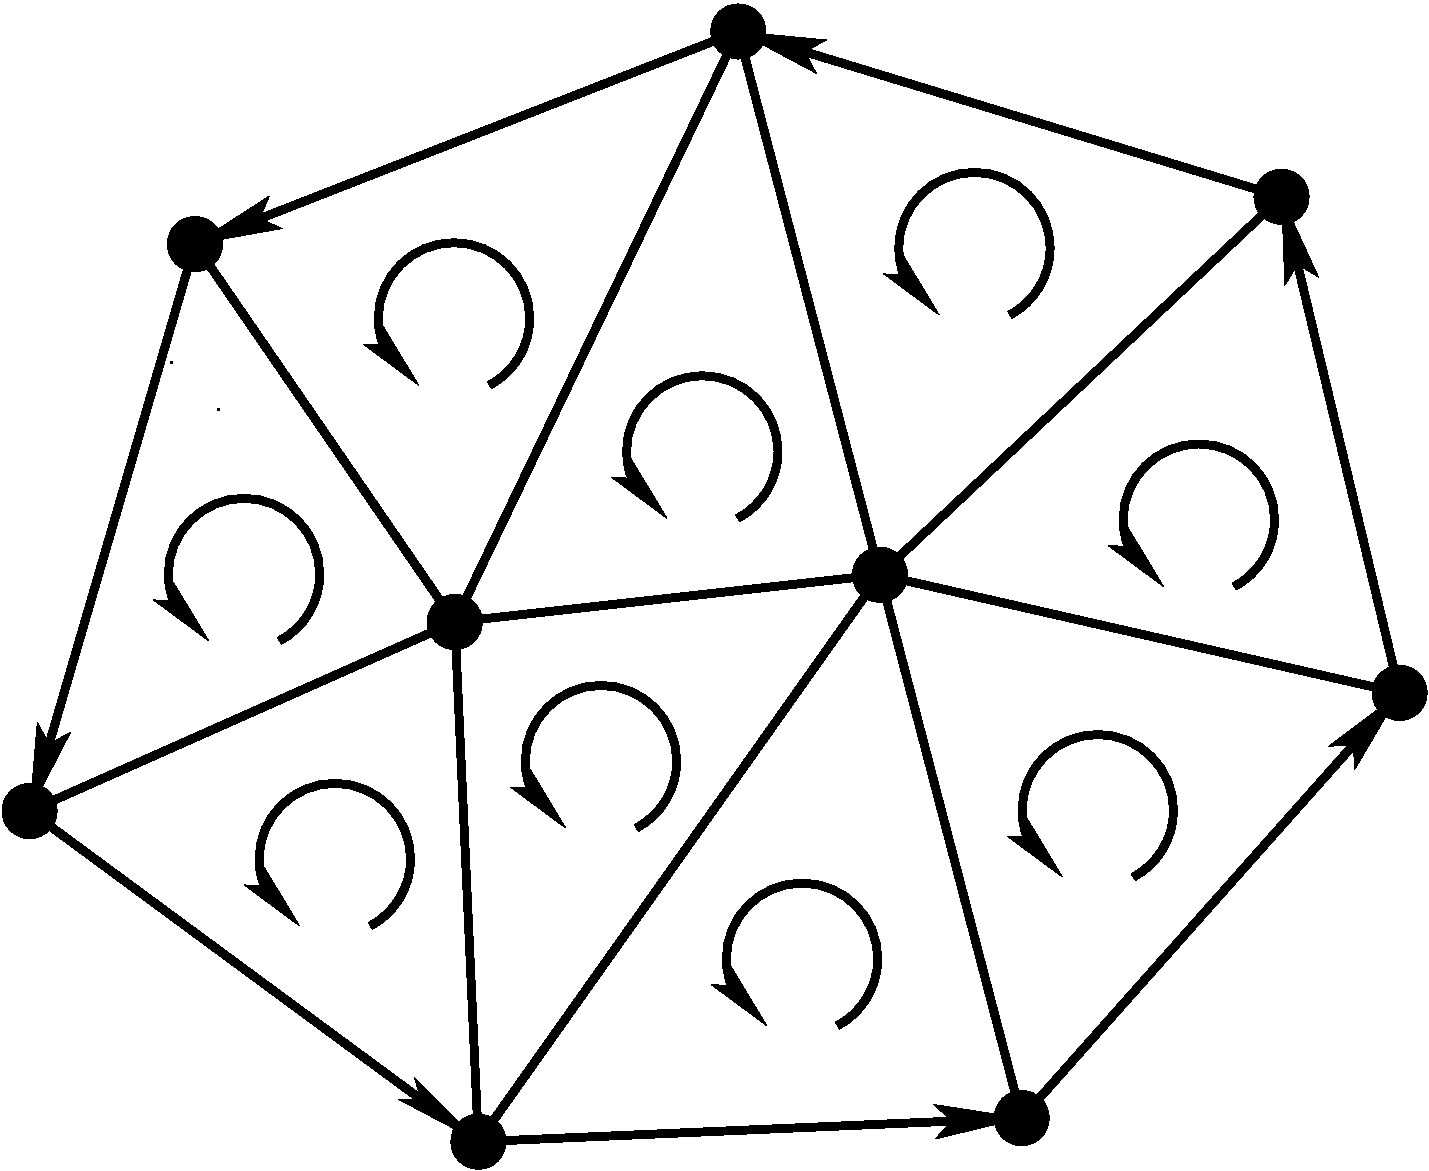
\includegraphics{simplex.png}}
\caption{Triangulated Surface}
\end{center}
\end{figure}
Each triangle in the surface is described by a planar simplex as shown
\begin{figure}[htbp]
\begin{center}
\scalebox{0.5}{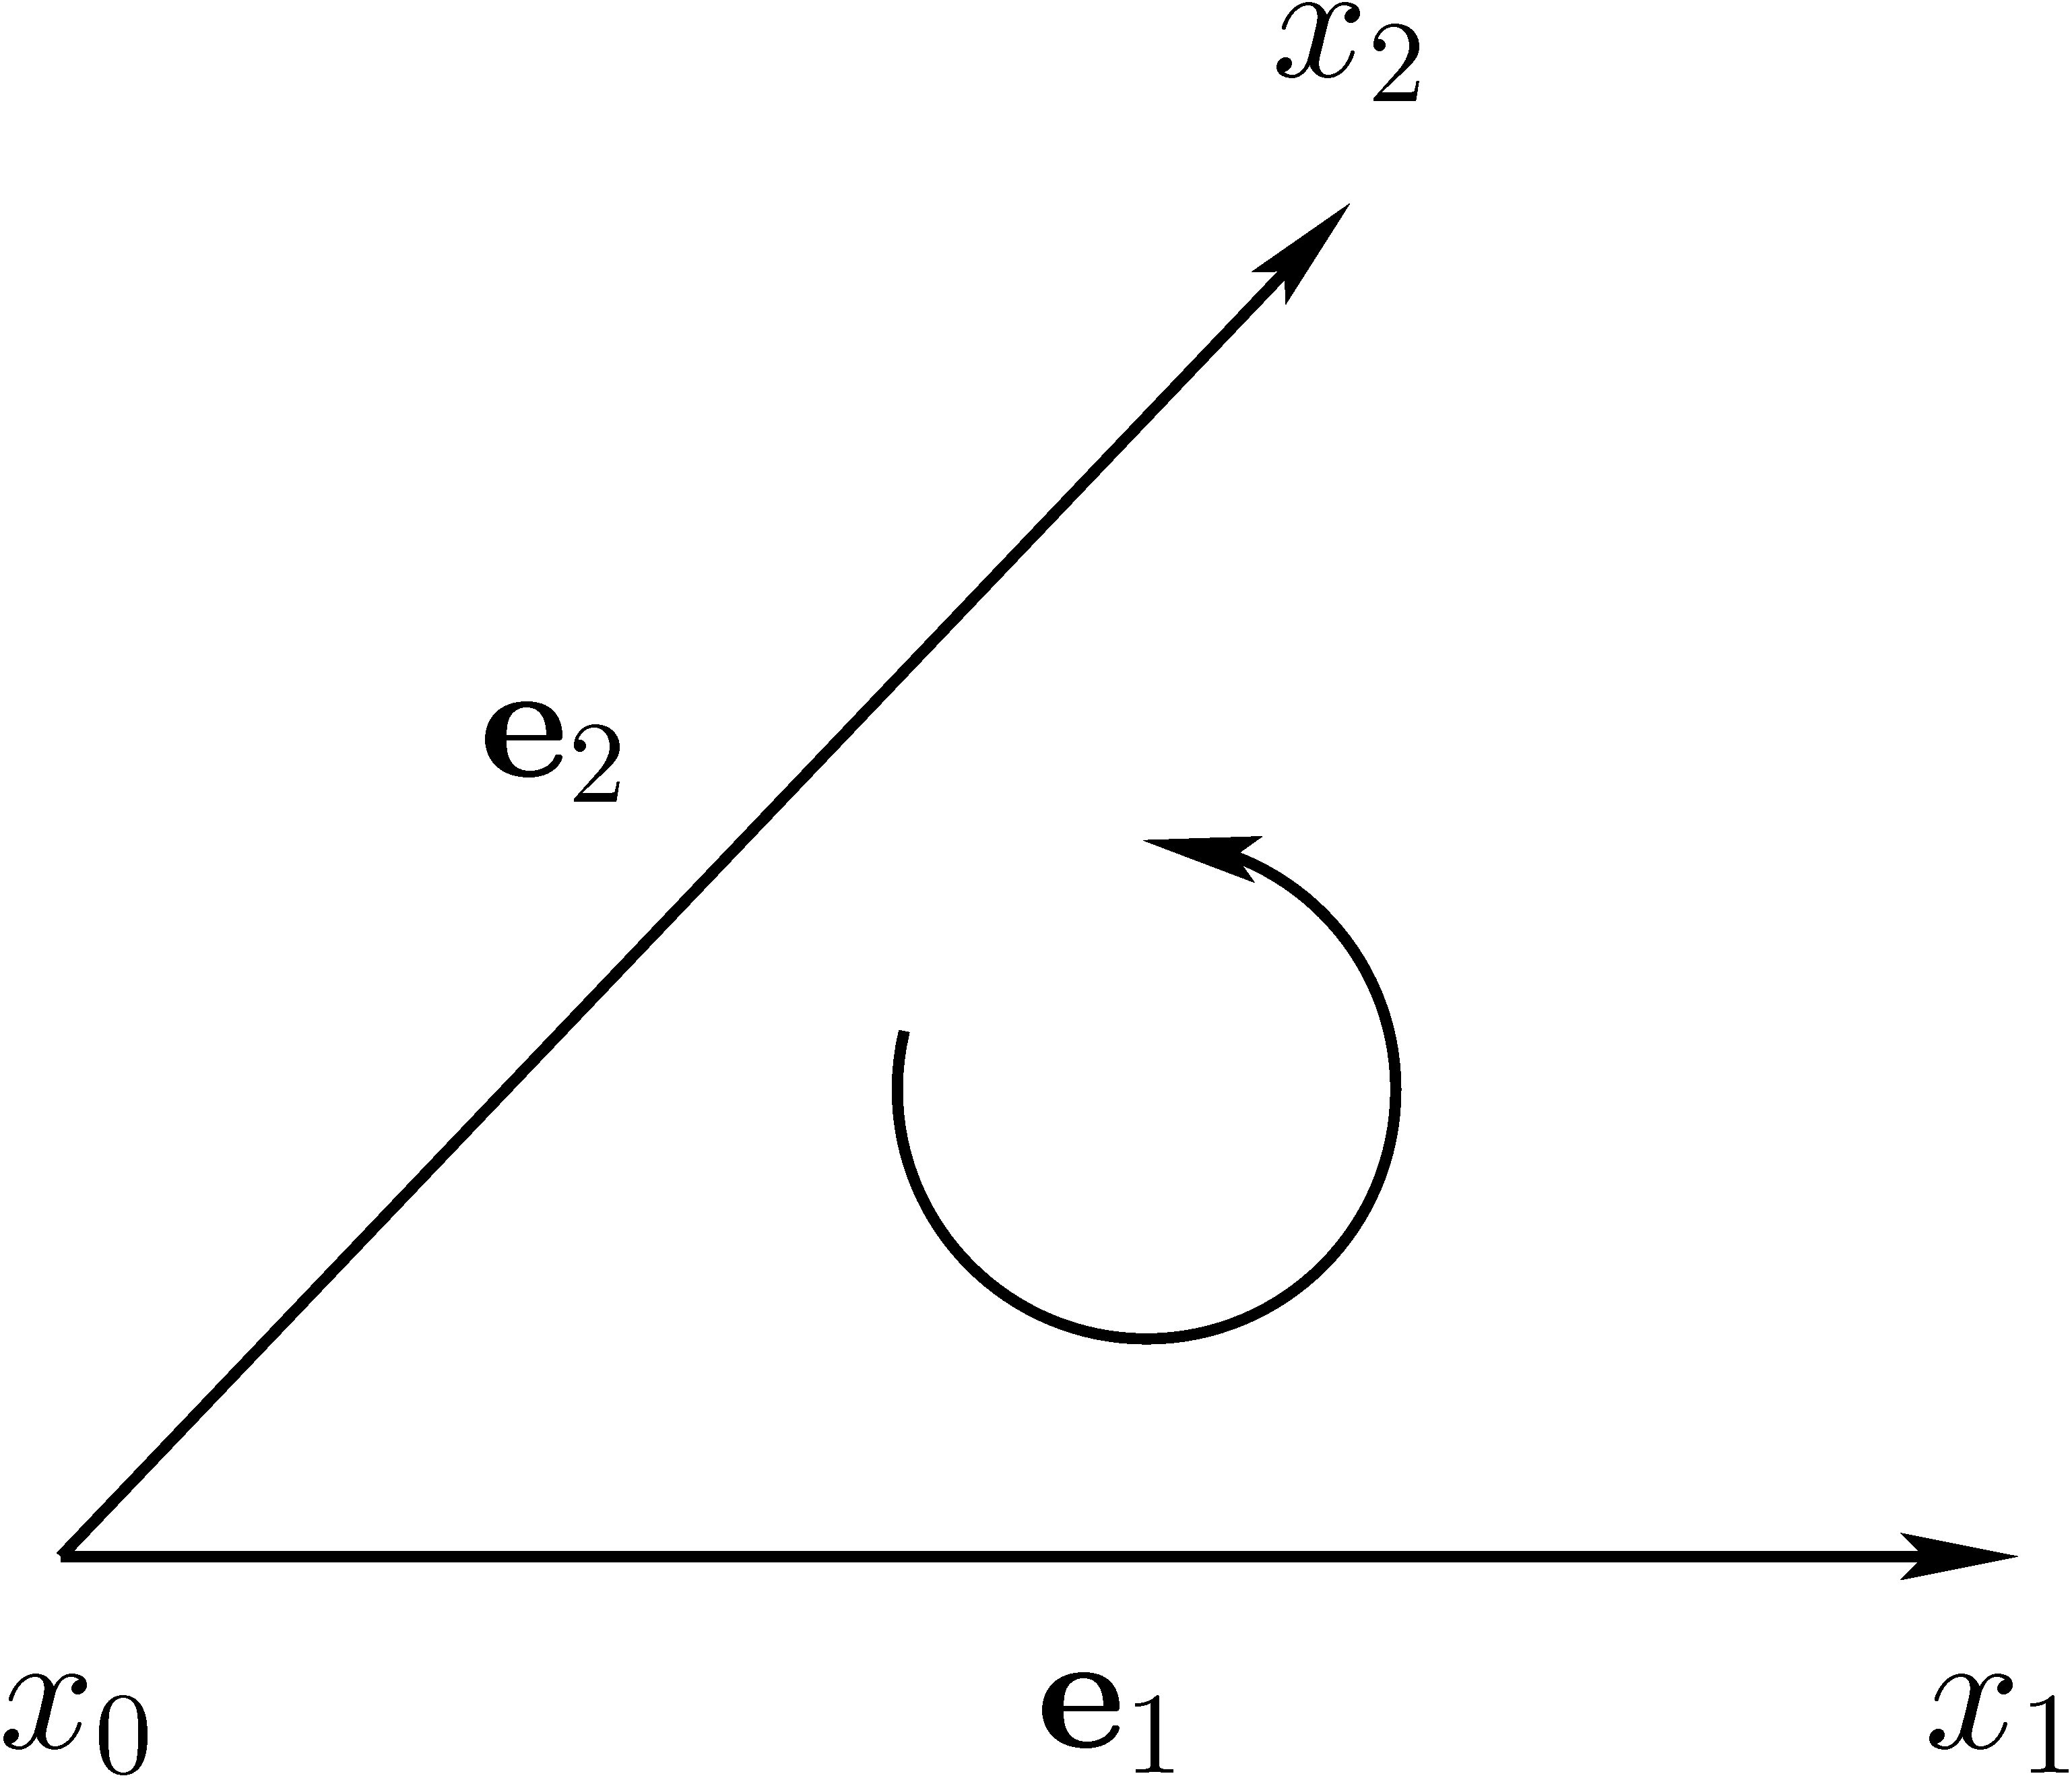
\includegraphics{planarsimplex.png}}
\caption{Planar Simplex}
\end{center}
\end{figure}
The three vertices of the planar simplex are $x_{0}$, $x_{1}$, and $x_{2}$ with the vectors
$\eb_{1}$ and $\eb_{2}$ defined by
\be
\begin{array}{cc}
\eb_{1} = x_{1}-x_{0}, & \eb_{2} = x_{2}-x_{0}
\end{array}
\ee
so that the surface measure of the simplex is
\be
\Delta X \equiv \half\eb_{1}\w\eb_{2} = \half\paren{x_{1}\w x_{2}+x_{2}\w x_{0}+x_{0}\w x_{1}}
\ee
with this definition of $\Delta X$ we have
\be
\int F\: dX  \equiv \lim_{n\mapsto\infty} \sum_{k=1}^{n} \bar{F}^{k}\Delta X^{k} 
\ee
where $\bar{F}^{k}$ is the average of $F$ over the $k^{th}$ simplex.
\section{Directed Integration - $n$-dimensional Surfaces}

\subsection{$k$-Simplex Definition}

In geometry, a simplex or $k$-simplex is an $k$-dimensional analogue of a triangle. Specifically, a simplex is the 
convex hull of a set of $(k + 1)$ affinely independent points in some Euclidean space of dimension $k$ or higher.

For example, a 0-simplex is a point, a 1-simplex is a line segment, a 2-simplex is a triangle, a 3-simplex is a 
tetrahedron, and a 4-simplex is a pentachoron (in each case including the interior).
A regular simplex is a simplex that is also a regular polytope. A regular $k$-simplex may be constructed from a regular 
$(k-1)$-simplex by connecting a new vertex to all original vertices by the common edge length.

\subsection{$k$-Chain Definition (Algebraic Topology)}

A finite set of $k$-simplexes embedded in an open subset of $\Re^{n}$ is called an affine $k$-chain. The simplexes in a
chain need not be unique, they may occur with multiplicity. Rather than using standard set notation to denote an affine 
chain, the standard practice to use plus signs to separate each member in the set. If some of the simplexes
have the opposite orientation, these are prefixed by a minus sign. If some of the simplexes occur in the set more than once,
these are prefixed with an integer count. Thus, an affine chain takes the symbolic form of a sum with integer coefficients.

\subsection{Simplex Notation}

If $\paren{x_{0},x_{1},\dots,x_{k}}$ is the $k$-simplex defined by the $k+1$ points 
$x_{0},x_{1},\dots,x_{k}$.  This is abbreviated by
\be
\chn{x}{k} = \paren{x_{0},x_{1},\dots,x_{k}}
\ee 
The order of the points is important for a simplex, since it specifies the orientation of the simplex.  If any two
adjacent points are swapped the simplex orientation changes sign.  The boundary operator for the simplex is denoted by $\partial$
and defined by
\be\label{eq211}
\partial\chn{x}{k} \equiv \sum_{i=0}^{k} \paren{-1}^{i}\chn{x_{0},\dots,\breve{x}_{i},\dots,x_{k}}{k-1}
\ee
To see that this make sense consider a triangle $\chn{x}{3} = \paren{x_{0},x_{1},x_{2}}$. Then
\begin{align}
\partial\chn{x}{3} &= \chn{x_{1},x_{2}}{2}-\chn{x_{0},x_{2}}{2}+\chn{x_{0},x_{1}}{2} \nonumber \\
                   &= \chn{x_{1},x_{2}}{2}+\chn{x_{2},x_{0}}{2}+\chn{x_{0},x_{1}}{2}
\end{align}
each 2-simplex in the boundary 2-chain connects head to tail with the same sign.

Now consider the boundary of the boundary
\begin{align}
\partial^{2}\chn{x}{3} &= \partial\chn{x_{1},x_{2}}{2}+\partial\chn{x_{2},x_{0}}{2}+\partial\chn{x_{0},x_{1}}{2}
                                \nonumber \\
                       &= \chn{x_{1}}{1}-\chn{x_{2}}{1}+\chn{x_{2}}{1}-\chn{x_{0}}{1}+\chn{x_{0}}{1}
                                 -\chn{x_{1}}{1} \nonumber \\
                       &= 0
\end{align}
We need to prove is that in general $\partial^{2}\chn{x}{k}=0$. To do this consider the boundary of the $i^{th}$
term on thr r.h.s. of equation~\ref{eq211} letting 
$\Aijk{ij}{k-2}= \chn{x_{0},\dots,\breve{x}_{i},\dots,\breve{x}_{j},\dots,x_{k}}{k-1}$. 

Then
\be\label{eq214}
\begin{array}{l}
\hspace{-0.25in}\partial\chn{x_{0},\dots,\breve{x}_{i},\dots,x_{k}}{k-1} = \\ 
 \hspace{0.2in}\left \{\begin{array}{cc}
 i = 0: & {\ds \sum_{j=1}^{k}\paren{-1}^{j-1}\Aijk{ij}{k-2} } \\
 0<i<k: & {\ds \sum_{j=0}^{i-1}\paren{-1}^{j}\Aijk{ij}{k-2}+\sum_{j=i+1}^{k}\paren{-1}^{j-1}\Aijk{ij}{k-2} } \\
 i = k: & {\ds \sum_{j=0}^{k-1}\paren{-1}^{j}\Aijk{ij}{k-2} }
\end{array}\right \}
\end{array} 
\ee
The critical point in equation~\ref{eq214} is that the exponent of $-1$ in the second term on the r.h.s. is
not $j$, but $j-1$.  The reason for this is that when $x_{i}$ was removed from the simplex the vertices were
{\bf not} renumbered.  We can now express the boundary of the boundary in terms of the following matrix elements
($\Bijk{ij}{k-2} = \paren{-1}^{i+j}\Aijk{ij}{k-2}$) as
\begin{align}\label{eq248}
\partial^{2}\chn{x}{k} = & \sum_{j=1}^{k}\paren{-1}^{j-1}\Aijk{0j}{k-2}+\paren{-1}^{k}\sum_{j=0}^{k-1}\paren{-1}^{j}\Aijk{kj}{k-2} \nonumber \\
                         & +\sum_{i=1}^{k-1}\paren{-1}^{i}\left(\sum_{j=0}^{i-1}\paren{-1}^{j}\Aijk{ij}{k-2}
                            +\sum_{j=i+1}^{k}\paren{-1}^{j-1}\Aijk{ij}{k-2} \right) \nonumber \\
                       = & -\sum_{j=1}^{k}\Bijk{0j}{k-2}+\sum_{j=0}^{k-1}\Bijk{kj}{k-2} \nonumber \\ 
                       & +\sum_{i=1}^{k-1}\sum_{j=0}^{i-1}\Bijk{ij}{k-2}-\sum_{i=1}^{k-1}\sum_{j=i+1}^{k}\Bijk{ij}{k-2} = 0
\end{align}
The consider $\Bijk{ij}{k-2}$ as a matrix ($i$-row index, $j$-column index). The matrix is symmetrical and in equation~\ref{eq248} you
are subtracting all the elements above the main diagonal from the elements below the main diagonal so that $\partial^{2}\chn{x}{k} = 0$ and
the boundary of a boundary of a simplex is zero.

Now add geometry to the simplex by defining the vectors
\be
\begin{array}{cc}
e_{i} = x_{i}-x_{0}, & i=1,\dots,k,
\end{array}
\ee
and the directed volume element
\be\label{eq196}
\Delta X = \bfrac{1}{k!}e_{1}\w\cdots\w e_{k}
\ee
We now wish to prove that
\be
\int_{\smplx{x}{k}} dX = \Delta X
\ee
Any point in the simplex can be written in terms of the coordinates $\ldi{i}$ as
\be\label{eq237}
x = x_{0}+\sum_{i=1}^{k} \ldi{i}e_{i}
\ee
with restrictions
\be
\begin{array}{ccc}
0\le\ldi{i}\le 1 & \mbox{and} & {\ds\sum_{i=1}^{k}\ldi{i} \le 1}
\end{array}
\ee
First we show that
\be
\int_{\smplx{x}{k}} dX = \int_{\smplx{x}{k}} e_{1}\w\cdots\w e_{k}\: \dldi{1}\cdots\dldi{k} = \Delta X
\ee
or
\be
\int_{\smplx{x}{k}} \dldi{1}\cdots\dldi{k} = \bfrac{1}{k!}
\ee
define $\Ldi{j}=1-\sum_{i=1}^{j}\ldi{i}$ (Note that $\Ldi{0}=1$). From the restrictions on the $\ldi{i}$'s we have
\be\label{eq201}
\int_{\smplx{x}{k}} \dldi{1}\cdots\dldi{k} = \int_{0}^{\Ldi{0}}\dldi{1}\int_{0}^{\Ldi{1}}\dldi{2}\cdots
	\int_{0}^{\Ldi{k-1}}\dldi{k}
\ee
To prove that the r.h.s of equation~\ref{eq201} is $1/k!$ we form the following sequence and use induction
to prove that $V_{j}$ is the result of the first $j$ partial Integrations of equation~\ref{eq201}
\be
V_{j} = \bfrac{1}{j!}\paren{\Ldi{k-j}}^{j}
\ee
Then
\begin{align}
V_{j+1} &= \int_{0}^{\Ldi{k-j-1}} \dldi{k-j}V_{j} \nonumber \\
		&= \int_{0}^{\Ldi{k-j-1}} \dldi{k-j}\bfrac{1}{j!}\paren{\Ldi{k-j-1}-\ldi{k-j}}^{j}
			\nonumber \\
        &= \bfrac{-1}{\paren{j+1}j!}\left[\paren{\Ldi{k-j-1}-\ldi{k-j}}^{j+1}
            \right]_{0}^{\Ldi{k-j-1}} \nonumber \\
        &=  \bfrac{1}{\paren{j+1}!}\paren{\Ldi{k-j-1}}^{j+1}\label{eq243}
\end{align}
so that $V_{k} = 1/k!$ and the assertion is proved.
Now let there be a multivector field $\fof{F}{x}$ that assumes the values $F_{i} = \fof{F}{x_{i}}$ at the vertices
of the simplex and define the interpolating function
\be\label{eq244}
\fof{f}{x} = F_{0}+\sum_{i=1}^{k}\ldi{i}\paren{F_{i}-F_{0}}
\ee
We now wish to show that
\be\label{eq205}
\int_{\smplx{x}{k}}f\: dX = \bfrac{1}{k+1}\paren{\sum_{i=0}^{k}F_{i}}\Delta X = \bar{F}\: \Delta X
\ee
To prove this we must show that
\be\label{eq206}
\int_{\smplx{x}{k}}\ldi{i}\: dX = \bfrac{1}{k+1} \Delta X,\quad \forall\:\ldi{i}
\ee
To do this consider the integral (equation~\ref{eq243} with $V_{j}$ replaced by $\ldi{k-j}V_{j}$) 
\begin{align}
\int_{0}^{\Ldi{k-j-1}}\dldi{k-j}\:\ldi{k-j}V_{j} &= \int_{0}^{\Ldi{k-j-1}}
		\dldi{k-j}\bfrac{1}{j!}\ldi{k-j}\paren{\Ldi{k-j-1}-\ldi{k-j}}^{j} \nonumber \\
	&= \bfrac{1}{\paren{j+2}!}\paren{\Ldi{k-j-1}}^{j+2}
\end{align}
Note that since the extra $\ldi{i}$ factor occurs in exactly one of the subintegrals for each different $\ldi{i}$ the
final result of the total integral is multiplied by a factor of $\frac{1}{\paren{k+1}}$ since the weight of the total integral 
is now $\frac{1}{\paren{k+1}!}$ and the assertion (equation~\ref{eq206} and hence equation~\ref{eq205}) is proved.

Now summing over all the simplices making up the directed volume gives
\be\label{eq208}
\int_{\mbox{volume}} F\: dX = \lim_{n\mapsto\infty} \sum_{i=1}^{n}\bar{F}^{i} \Delta X^{i}
\ee
The most general statement of equation~\ref{eq208} is
\be
\int_{\mbox{volume}} \fof{\mathsf{L}}{dX} = \lim_{n\mapsto\infty} \sum_{i=1}^{n}\fof{\bar{\mathsf{L}}^{i}}{\Delta X^{i}}
\ee
where $\fof{\mathsf{L}}{F_{n};x}$ is a position dependent linear function of a grade-$n$ multivector $F_{n}$ and 
$\bar{\mathsf{L}}^{i}$ is the average value of $\fof{\mathsf{L}}{dX}$ over the vertices of each simplex.

An example of this would be
\be
	\fof{\mathsf{L}}{F_{n};x} = \fof{G}{x} F_{n} \fof{H}{x} 
\ee
where $\fof{G}{x}$ and $\fof{H}{x}$ are multivector functions of $x$.
\section{Fundamental Theorem of Geometric Calculus}
Now prove that the directed measure of a simplex boundary is zero 
\be\label{eq218}
\Delta\paren{\partial\chn{x}{k}} = \Delta\paren{\partial\chn{x_{0},\dots,x_{k}}{k}} = 0
\ee
Start with a planar simplex of three points
\be
\partial\chn{x_{0},x_{1},x_{2}}{2} = \chn{x_{1},x_{2}}{1}-\chn{x_{0},x_{2}}{1}+\chn{x_{0},x_{1}}{1}
\ee
so that
\be
\Delta\paren{\partial\chn{x_{0},x_{1},x_{2}}{2}} = \paren{x_{2}-x_{1}}-\paren{x_{2}-x_{0}}+\paren{x_{1}-x_{0}} = 0
\ee
We shall now prove equation~\ref{eq218} via induction.  First note that
\be
\Delta\chn{\breve{x}_{i}}{k-1} = \left\lbrace
\begin{array}{cc}
i = 0: & \bfrac{1}{k-1}\Delta\chn{\breve{x}_{0}}{k-2}\w\paren{x_{k}-x_{1}} \\
0 < i \le k-1: & \bfrac{1}{k-1}\Delta\chn{\breve{x}_{i}}{k-2}\w\paren{x_{k}-x_{0}}
\end{array}
 \right\rbrace 
\ee
and
\be
\Delta\chn{\breve{x}_{k}}{k-1} = \bfrac{1}{\paren{k-1}!}\paren{x_{1}-x_{0}}\W\cdots\W\paren{x_{k-1}-x_{0}}
\ee
so that
\be
\Delta\paren{\partial\chn{x}{k}} = 
   \bfrac{1}{k-1}\sum_{i=1}^{k-1}\paren{-1}^{i}\Delta\chn{\breve{x}_{i}}{k-2}\w\paren{x_{k}-x_{0}}+\mathcal{C} \nonumber \\
\ee
where
\be
\mathcal{C} = \bfrac{1}{k-1}\Delta\chn{\breve{x}_{0}}{k-2}\w\paren{x_{k}-x_{1}}
+\paren{-1}^{k}\Delta\chn{\breve{x}_{k}}{k-1}
\ee
if we let $\delta = x_{0}-x_{1}$ we can write
\be
\mathcal{C} = \bfrac{1}{k-1}\Delta\chn{\breve{x}_{0}}{k-2}\w\paren{x_{k}-x_{0}}+
               \bfrac{1}{k-1}\Delta\chn{\breve{x}_{0}}{k-2}\w\delta
              +\paren{-1}^{k}\Delta\chn{\breve{x}_{k}}{k-1}
\ee
Then
\begin{align}
\Delta\chn{\breve{x}_{0}}{k-2}\w\delta &= \bfrac{1}{\paren{k-2}!}\paren{x_{2}-x_{1}}\W\cdots\W\paren{x_{k-1}-x_{1}}\W\delta \\
                                       &= \bfrac{1}{\paren{k-2}!}\paren{x_{2}-x_{0}+\delta}\W\cdots\W\paren{x_{k-1}-x_{0}+\delta}\W\delta \\
                                       &= \bfrac{1}{\paren{k-2}!}\paren{x_{2}-x_{0}}\W\cdots\W\paren{x_{k-1}-x_{0}}\W\delta \\
                                       &= \bfrac{\paren{-1}^{k-2}}{\paren{k-2}!}\delta\W\paren{x_{2}-x_{0}}\W\cdots\W\paren{x_{k-1}-x_{0}} \\                                                                    									   &= \bfrac{\paren{-1}^{k-1}}{\paren{k-2}!}\paren{x_{1}-x_{0}}\W\paren{x_{2}-x_{0}}\W\cdots\W\paren{x_{k-1}-x_{0}}
\end{align}
Thus
\begin{align}
\bfrac{-1}{k-1}\Delta\chn{\breve{x}_{0}}{k-2}\w\delta &= \\
                                                      &\hspace{-1.5in}= \bfrac{\paren{-1}^{k}}{\paren{k-1}!}\paren{x_{1}-x_{0}}\W\paren{x_{2}-x_{0}}\W\cdots\W\paren{x_{k-1}-x_{0}} \\
                                                      &\hspace{-1.5in}= \paren{-1}^{k}\Delta\chn{\breve{x}_{k}}{k-1}
\end{align}
However
\be
\paren{-1}^{k}\Delta\chn{\breve{x}_{k}}{k-1} = \bfrac{-1}{k-1}\Delta\chn{\breve{x}_{0}}{k-2}\w\delta
\ee
so that
\be\label{eq226}
\mathcal{C} = \bfrac{1}{k-1}\Delta\chn{\breve{x}_{0}}{k-2}\w\paren{x_{k}-x_{0}}
\ee
and
\begin{align}
\Delta\paren{\partial\chn{x}{k}} &=\bfrac{1}{k-1}\paren{\sum_{i=0}^{k-1}\paren{-1}^{i}\Delta\chn{\breve{x}_{i}}{k-2}}
                                   \w\paren{x_{k}-x_{0}} \nonumber \\
                                 &= \bfrac{1}{k-1}\paren{\Delta\paren{\partial\chn{x}{k-1}}}
                                     \w\paren{x_{k}-x_{0}} \nonumber \\
                                 &= 0
\end{align}
We have proved equation~\ref{eq218}.  Note that to reduce equation~\ref{eq226} we had to use that for any set of vectors $\delta,y_{1},\dots,y_{k}$ we have
\be\label{eq228}
\delta\w\paren{y_{1}+\delta}\w\cdots\w\paren{y_{k}+\delta} = \delta\w y_{1}\w\cdots\w y_{k}
\ee
Think about equation~\ref{eq228}. It's easy to prove ($\delta\W \delta = 0$)!

Equation~\ref{eq218} is sufficient to prove that the directed integral over the surface of simplex is
zero
\be
\oint_{\partial\chn{x}{k}}dS = \sum_{i=0}^{k}\paren{-1}^{i}\int_{\chn{\breve{x}_{i}}{k-1}}
                                              \hspace{-0.5in}dX = \Delta\paren{\partial\chn{x}{k}} = 0
\ee
The characteristics of a general volume are:
\begin{enumerate}
\item A general volume is built up from a chain of simplices.
\item Simplices in the chain are defined so that at any common boundary the directed
 areas of the bounding faces are equal and opposite.
\item Surface integrals over two simplices cancel over their common face.
\item The surface integral over the boundary of the volume can be replaced by the sum
of the surface integrals over each simplex in the chain.
\end{enumerate}
If the boundary of the volume is closed we have
\be\label{eq230}
\oint dS = \lim_{n\mapsto\infty}\sum_{a=1}^{n}\oint dS^{a} = 0 
\ee
Where $\oint dS^{a}$ is the surface Integral over the $a^{th}$ simplex. Implicit
in equation~\ref{eq230} is that the surface is orientated, simply connected, and 
closed.

The next lemma to prove that if $b$ is a constant vector on the simplex $\smplx{x}{k}$ then
\be\label{eq262}
\oint_{\partial\smplx{x}{k}} \hspace{-0.25in}b\cdot x\; dS = b\cdot\Delta\lp\smplx{x}{k}\rp = b\cdot\Delta X
\ee
The starting point of the lemma is equation~\ref{eq206}. First define
\be
 b = \sum_{i=1}^{k}b_{i}e^{i},
\ee
where the $e^{i}$'s are the reciprocal frame to $e_{i} = x_{i}-x_{0}$ so that
\be
x-x_{0}=\sum_{i=1}^{k}\lambda^{i}e_{i},
\ee
\be
b_{i}=b\cdot e_{i},
\ee
and
\be
\sum_{i=1}^{k}\ldi{i}b_{i}=b\cdot\lp x-x_{0}\rp.
\ee
Substituting into equation~\ref{eq206} we get
\be
\sum_{i=1}^{k}\int_{\smplx{x}{k}}\hspace{-0.25in}b_{i}\lambda^{i}\;dX = \int_{\smplx{x}{k}}\hspace{-0.25in}b\cdot\lp x-x_{0}\rp\;dX = 
         \bfrac{1}{k+1}\sum_{i=1}^{k}b\cdot e_{i}\; \Delta X
\ee
Rearranging terms gives
\begin{align}
	\int_{\smplx{x}{k}}\hspace{-0.25in}b\cdot x\;dX & = \bfrac{1}{k+1}\lp \lp\sum_{i=1}^{k}b\cdot\lp x_{i}-x_{0}\rp\rp
	                                                    +\lp k+1\rp b\cdot x_{0}\rp \Delta X \nonumber \\
                                                    & = \bfrac{b}{k+1}\cdot\lp\sum_{i=0}^{k} x_{i}\rp\Delta X \nonumber \\
                                                    & = b\cdot\bar{x}\Delta X\label{eq264}
\end{align}
Now using the definition of a simplex boundary (equation~\ref{eq211}) and equation~\ref{eq264} we get
\be
\hspace{-0.75in}\oint_{\partial\smplx{x}{k}}\hspace{-0.25in}b\cdot x\;dS = \bfrac{1}{k}\sum_{i=0}^{k}\lp -1\rp^{i}b\cdot
       \lp x_{0}+\cdots+\breve{x_{i}}+\cdots+x_{k}\rp\Delta\lp\smplx{\breve{x_{i}}}{k-1}\rp\label{eq265}
\ee
The coefficient multiplying the r.h.s. of equation~\ref{eq265} is $\bfrac{1}{k}$ and not $\bfrac{1}{k+1}$ because both\newline 
$\lp x_{0}+\cdots+\breve{x_{i}}+\cdots+x_{k}\rp$ and $\smplx{\breve{x_{i}}}{k-1}$ refer to $k-1$ simplices (the boundary of
$\smplx{x}{k}$ is the sum of all the simplices $\smplx{\breve{x_{i}}}{k}$ with proper sign assigned).

Now to prove equation~\ref{eq262} we need to prove one final purely algebraic lemma
\be\label{eq266}
 \hspace{-0.25in}\sum_{i=0}^{k}\lp -1\rp^{i}b\cdot\lp x_{0}+\cdots+\breve{x_{i}}+\cdots+x_{k}\rp\Delta\smplx{\breve{x_{i}}}{k-1} = 
      \bfrac{1}{\lp k-1\rp !}b\cdot\lp e_{1}\W\cdots\W e_{k}\rp
\ee
Begin with the definition of the l.h.s. of equation~\ref{eq266}
\be
\mathsf{C} = \sum_{i=0}^{k}\paren{-1}^{i}b\cdot\paren{x_{0}+\cdots+\breve{x}_{i}+\cdots +x_{k}}\Delta\chn{\breve{x}_{i}}{k-1} = \sum_{i=0}^{k}\mathsf{C}_{i}
\ee
where $\mathsf{C}_{i}$ is defined by
\be
\mathsf{C}_{i} = \left\lbrace \begin{array}{cc}
i = 0: & b\cdot\paren{x_{1}+\cdots+ x_{k}}\Delta\chn{\breve{x}_{0}}{k-1} \\
0<i \le k: & \paren{-1}^{i}b\cdot\paren{x_{0}+\cdots+\breve{x}_{i}+\cdots +x_{k}}\Delta\chn{\breve{x}_{i}}{k-1}
\end{array}
\right\rbrace 
\ee
now define $E_{k} = e_{1}\w\cdots\w e_{k}$ so that (using equation~\ref{eq61} from the section on reciprocal frames)
\be
\paren{-1}^{i-1}e^{i}E_{k}= e_{1}\w\cdots\w\breve{e}_{i}\w\cdots\w e_{k},\quad\forall\: 0< i \le k
\ee
and
\be
\mathsf{C}_{0<i\le k} =  \bfrac{-1}{\paren{k-1}!}b\cdot\paren{x_{0}+\cdots+\breve{x}_{i}+\cdots +x_{k}}e^{i}E_{k}
\ee
The main problem is in evaluating $\mathsf{C}_{0}$ since
\be\label{eq271}
\Delta\chn{\breve{x}_{0}}{k-1} = \bfrac{1}{\paren{k-1}!}\paren{x_{2}-x_{1}}\w\cdots\w\paren{x_{k}-x_{1}}
\ee
using $e_{i} = x_{i}-x_{0}$ reduces equation~\ref{eq271} to 
\be\label{eq272}
\Delta\chn{\breve{x}_{0}}{k-1} = \bfrac{1}{\paren{k-1}!}\paren{e_{2}-e_{1}}\w\cdots\w\paren{e_{k}-e_{1}}
\ee
but equation~\ref{eq272} can be expanded into equation~\ref{eq273}.  The critical point in doing the expansion is that
in generating the sum on the r.h.s. of the first line of equation~\ref{eq273} all products containing $x_{1}$ (of course 
all terms in the sum contain $x_{1}$ exactly once since we are using the outer product) are put in
normal order by bringing the $x_{1}$ factor to the front of the product thus requiring the factor of $\paren{-1}^{i}$
in each term in the sum. 
\begin{align}
\hspace{-0.5in}\paren{e_{2}-e_{1}}\w\cdots\w\paren{e_{k}-e_{1}} & = e_{2}\w\cdots\w e_{k} - \sum_{i=2}^{k}\paren{-1}^{i}
         e_{1}\w e_{2}\w\cdots\w\breve{e}_{i}\w\cdots\w e_{k} \nonumber \\
      & =  \sum_{i=1}^{k}\paren{-1}^{i-1}
         e_{1}\w e_{2}\w\cdots\w\breve{e}_{i}\w\cdots\w e_{k} \nonumber \\
      & =  \sum_{i=1}^{k}e^{i}E_{k} \label{eq273}
\end{align}
or
\be
\Delta\chn{\breve{x}_{0}}{k-1} = \bfrac{1}{\paren{k-1}!}\sum_{i=1}^{k}e^{i}E_{k}
\ee
from equation~\ref{eq273} we have
\begin{align}
\hspace{-0.5in}\mathsf{C} & = \bfrac{1}{\paren{k-1}!}\sum_{i=1}^{k} 
                                \paren{b\cdot\paren{x_{i}-x_{0}}}e^{i}E_{k} \nonumber \\
                          & = \bfrac{1}{\paren{k-1}!}\sum_{i=1}^{k}\paren{b\cdot e_{i}}e^{i}E_{k} \nonumber \\
                          & = \bfrac{1}{\paren{k-1}!}\sum_{i=1}^{k}b_{i}e^{i}E_{k} \nonumber \\
                          & = \bfrac{1}{\paren{k-1}!}bE_{k} \nonumber \\
                          & = \bfrac{1}{\paren{k-1}!}\paren{b\cdot E_{k}+ b\w E_{k}} \nonumber \\
                          & = \bfrac{1}{\paren{k-1}!}b\cdot E_{k} 
\end{align}
and equation~\ref{eq266} is proved which means substituting equation~\ref{eq266} into equation~\ref{eq265} proves equation~\ref{eq262}

\subsection{The Fundamental Theorem At Last!}

The simplicial coordinates, $\lambda^{i}$, can be expressed in terms of the position vector, $x$, and the frame vectors of the 
simplex, $e_{i} = x_{i}-x_{0}$. Let the vectors $e^{j}$ be the reciprocal frame to $e_{i}$ ($e_{i}\cdot e^{j} = \delta_{i}^{j}$).  Then
\be
\lambda^{i} = e^{i}\cdot\lp x-x_{0}\rp
\ee
and let $\f{f}{x}$ be an affine multivector function of $x$ (equation~\ref{eq244}) which interpolates, $F$, a differentiable multivector 
function of $x$ on the simplex. Then
\begin{align}
\oint_{\partial\smplx{x}{k}}\hspace{-0.25in}\f{f}{x}\;dS &= \sum_{i=1}^{k}\lp F_{i}-F_{0}\rp\oint_{\partial\smplx{x}{k}}\hspace{-0.25in}
                 e^{i}\cdot\lp x-x_{0}\rp dS \nonumber \\
                                                         &= \sum_{i=1}^{k}\lp F_{i}-F_{0}\rp e^{i}\cdot\lp\Delta X\rp\label{eq277}
\end{align}
But
\be
\pdiff{\f{f}{x}}{\lambda^{i}} = F_{i}-F_{0}
\ee
so that the surface integral of equation~\ref{eq277} can be rewritten
\begin{align}
\oint_{\partial\smplx{x}{k}}\hspace{-0.35in}\f{f}{x}\;dS &= \sum_{i=1}^{k}\lp F_{i}-F_{0}\rp e^{i}\cdot\lp\Delta X\rp \nonumber \\
                                                         &= \sum_{i=1}^{k}\pdiff{f}{\lambda^{i}}e^{i}\cdot\lp\Delta X\rp 
                                                          = \dot{f}\dot{\nabla}\cdot\lp \Delta X\rp\label{eq279}
\end{align}
If we now sum equation~\ref{eq279} over a chain of simplices realizing that the interpolated function $\f{f}{x}$ takes on the same value
over the common boundary of two adjacent simplices, since $\f{f}{x}$ is only defined by the values at the common vertices.  In forming a
sum over a chain, all of the internal faces cancel and only the surface integral over the boundary remains.  Thus
\be
\oint\f{f}{x}\;dS = \sum_{a}\dot{f}\dot{\nabla}\cdot\lp\Delta X^{a} \rp
\ee
with the sum running over all simplices in the chain.  Taking the limit as more points are added and each simplex is shrunk in size we obtain
the first realization of the fundamental theorem of geometric calculus
\be\label{FTGC0}
\oint_{\partial V} F\; dS = \int_{V}\dot{F}\dot{\nabla}\;dX
\ee
We can write $\nabla dX$ instead of $\nabla \cdot dX$ since the vector $\nabla$ is totally within the vector space defined by $dX$ so that
$\nabla\W dX=0$.
The method of proof used can also be applied to the form
\be\label{FTGC1}
\oint_{\partial V}dS\;G = \int_{V}\dot{\nabla}\;dX\;\dot{G}
\ee
A more general statement of the theorem is as follows:

Let $\Llin\lp A_{k-1}\rp = \Llin\lp A_{k-1};x\rp$ be a linear functional of a multivector $A_{k-1}$ of grade $k-1$ and a general function of 
position $x$ which returns a general multivector.  The linear interpolation (approximation) of $\Llin$ over a simplex is defined by:
\be
\f{L}{A} \equiv \Llin\lp A;x_{0}\rp+\sum_{i=1}^{k}\lambda^{i}\lp \Llin\lp A;x_{i}\rp- \Llin\lp A;x_{0}\rp\rp
\ee
Then the integral over a simplex is (Note that since integration is a linear operation, a summation, the integral can be placed inside $\f{L}{A}$ since $\f{L}{A}$
is linear in $A$)
\begin{align}
\oint_{\partial\smplx{x}{k}} \f{L}{dS} &= \f{\Llin}{\oint dS;x_{0}}+\sum_{i=1}^{k}\f{\Llin}{\oint \lambda^{i}dS;x_{i}}-\sum_{i=1}^{k}\f{\Llin}{\oint \lambda^{i}dS;x_{0}} \nonumber \\
                &= \sum_{i=1}^{k}\lp\f{\Llin}{e^{i}\Delta X;x_{i}}-\f{\Llin}{e^{i}\Delta X;x_{0}}\rp \nonumber \\
                &= \f{\dot{L}}{\dot{\nabla}\Delta X}
\end{align}
Taking the limit of a sum of simplicies gives
\be\label{FTGC}
\oint_{\partial V}\f{\Llin}{dS} = \int_{V}\f{\dot{\Llin}}{\dot{\nabla}dX}
\ee
\section{Examples of the Fundamental Theorem}
\subsection{Divergence and Green's Theorems}
As a specific example consider $\f{\Llin}{A} = \grdO{JAI^{-1}}$ where $J$ is a vector, $I$ is the unit pseudoscalar for a $n$-dimensional
vector space, and $A$ is a multivector of grade $n-1$.  Then equation~\ref{FTGC} gives
\be               
\int_{V}\grdO{\dot{J}\dot{\nabla}dXI^{-1}} = \int_{V}\nabla\cdot J\abs{dX} = \oint_{\partial V}\grdO{JdSI^{-1}}
\ee
we have $dX = I\abs{dX}$ where $\abs{dX}$ is the scalar measure of the volume.  The normal to the surface, $n$, is defined by
\be
n\abs{dS} = dSI^{-1}
\ee
where $\abs{dS}$ is the scalar valued measure over the surface.  With this definition we get
\be\label{eq_divth}
\int_{V}\nabla\cdot J \abs{dX} = \oint_{\partial V}n\cdot J \abs{dS}
\ee

Now using the form of the Fundamental Theorem of Geometric Calculus in equation~\ref{FTGC1} and let $G$ be the vector
$\bm{J}$ in two-dimensional Euclidean space and noting that since $dA$ is a pseudoscalar (for 2-D $ds$ is the boundary measure 
and $dA$ is the volume measure) it anticommutes with vectors in
two dimensions we get -
\be
\oint_{\partial A}ds \bm{J} = \int_{A}\bm{\dot{\nabla}}dA\bm{\dot{J}} = -\int_{A}\bm{\nabla J}dA
\ee
In 2-D Cartesian coordinates $dA = Idxdy$ and $ds = nI\abs{ds}$ so that 
\be
\oint_{\partial A}ds\bm{J} = -\int_{A}\bm{\nabla \bm{J}}Idxdy.
\ee
or
\begin{align}
\oint_{\partial A}nI\bm{J}\abs{ds} &= -\int_{A}\bm{\nabla \bm{J}}Idxdy \nonumber \\
-\oint_{\partial A}n\bm{J}I\abs{ds} &= -\int_{A}\bm{\nabla \bm{J}}Idxdy \\
\oint_{\partial A}n\bm{J}\abs{ds} &= \int_{A}\bm{\nabla \bm{J}}dxdy
\end{align}
Letting $\bm{J} = P\bm{e}_{x}+Q\bm{e}_{y}$ and $n=n^{x}\bm{e}_{x}+n^{y}\bm{e}_{y}$ we get -
\begin{align}
n\bm{J} &= n\cdot\bm{J}+\paren{n^{x}Q-n^{y}P}\bm{e}_{x}\bm{e}_{y} \\
\nabla \bm{J} &= \nabla\cdot\bm{J}+\paren{\pdiff{Q}{x}-\pdiff{P}{y}}\bm{e}_{x}\bm{e}_{y}
\end{align}
so that
\begin{align}
\oint_{\partial A}n\cdot\bm{J}\abs{ds} &= \int_{A}\nabla\cdot\bm{J}dxdy \\
\oint_{\partial A}\paren{n^{x}Q-n^{y}P}\abs{ds}\bm{e}_{x}\bm{e}_{y} &= \int_{A}\paren{\pdiff{Q}{x}-\pdiff{P}{y}}dxdy\bm{e}_{x}\bm{e}_{y}
\end{align}
but $dy = n^{x}\abs{ds}$ and $dx = -n^{y}\abs{ds}$ so that
\be
\oint_{\partial A} Pdx+Qdy = \int_{A} \lp\pdiff{Q}{x}-\pdiff{P}{y}\rp dxdy
\ee
which is Green's theorem in the plane.

\subsection{Cauchy's Integral Formula In Two Dimensions (Complex Plane)}
Consider a two dimensional euclidean space with vectors $\bm{r} = x\bm{e}_{x}+y\bm{e}_{y}$.  Then the complex number $z$ corresponding to $\bm{r}$ is
\begin{align}
 z  &= \bm{e}_{x}\bm{r} = x + y\bm{e}_{x}\bm{e}_{y} = x + yI \\
 z^{\R} &= \bm{r}\bm{e}_{x} = x - y\bm{e}_{x}\bm{e}_{y} = x - yI \\
 zz^{\R } &= z^{\R }z = x^{2}+y^{2} = \bm{r}^{2}
\end{align}
Thus even grade multivectors correspond to complex numbers since $I^{2}=-1$ and the reverse of $z$, $z^{\R}$ corresponds to the conjugate of $z$.
Even grade multivectors commute with $dS$, since $dS$ is proportional to $I$.

Let $\f{\psi}{\bm{r}}$ be an even multivector function of $\bm{r}$, then
\be
	\int\bm{\nabla}\psi dS = \oint d\bm{s}\psi = \oint\pdiff{\bm{r}}{\lambda}\psi d\lambda
\ee
but the complex number $z$ is given by $z=\bm{e}_{x}\bm{r}$ and
\be
\bm{e}_{x}\oint d\bm{s}\psi = \oint \psi dz = \int\bm{e}_{x}\bm{\nabla}\psi dS.
\ee
Thus if a function $\psi$ is analytic, $\bm{\nabla}\psi = 0$ and $\oint \psi dz = 0$.  Now note that (this will be proved for the N-dimensional case in the next
example)
\be
\bm{\nabla}\bfrac{\bm{r-a}}{\paren{\bm{r-a}}^{2}} = 2\pi\f{\delta}{\bm{r-a}}
\ee
where $a = \bm{e}_{x}\bm{a}$.  Now let
\be
\psi = \bfrac{\bm{r-a}}{\paren{\bm{r-a}}^{2}}\bm{e}_{x}\f{f}{\bm{e}_{x}\bm{r}}
\ee
so that
\begin{align}
\bm{e}_{x}\oint d\bm{s}\psi &=  \bm{e}_{x}\oint d\bm{s}\lp \bfrac{\bm{r-a}}{\paren{\bm{r-a}}^{2}}\bm{e}_{x}\f{f}{\bm{e}_{x}\bm{r}}\rp \nonumber \\
                            &=  \oint dz\lp \bfrac{\bm{r-a}}{\paren{\bm{r-a}}^{2}}\bm{e}_{x}\f{f}{\bm{e}_{x}\bm{r}}\rp \nonumber \\
                            &=  \oint dz\lp \bfrac{\lp z-a\rp^{\dagger}}{\lp z-a\rp \lp z-a\rp^{\dagger}}\f{f}{z}\rp \nonumber \\
                            &=  \oint \bfrac{\f{f}{z}}{z-a} dz
\end{align}
and
\begin{align}
\oint\bfrac{\f{f}{z}}{z-a}dz &= \bm{e}_{x}\int\f{\bm{\nabla}}{\bfrac{\bm{r-a}}{\paren{\bm{r-a}}^{2}}\bm{e}_{x}\f{f}{\bm{e}_{x}\bm{r}}}dS \nonumber \\
                             &= \bm{e}_{x}\int\lp 2\pi\f{\delta}{\bm{r-a}}\bm{e}_{x}\f{f}{\bm{e}_{x}\bm{r}}+\bm{\nabla}\f{f}{\bm{e}_{x}\bm{r}}\bfrac{\bm{r-a}}{\paren{\bm{r-a}}^{2}}\bm{e}_{x}\rp I\abs{dS} \nonumber \\
                             &= 2\pi I\fct{f}{a}+\int\bm{e}_{x}\bm{\nabla}\f{f}{\bm{e}_{x}\bm{r}}\bfrac{z^{\dagger}-a^{\dagger}}{\abs{z-a}^{2}}I\abs{dS} \nonumber \\
                             &= 2\pi I\fct{f}{a}+\int\bm{e}_{x}\bm{\nabla}\f{f}{\bm{e}_{x}\bm{r}}\bfrac{1}{z-a}I\abs{dS} \nonumber \\
                             &= 2\pi I\fct{f}{a}+\int\lp\pdiff{}{x}+I\pdiff{}{y}\rp\f{f}{z}\bfrac{1}{z-a}I\abs{dS}
\end{align}
If $\bm{\nabla}\f{f}{z}=0$ we have -
\be
\oint\bfrac{\f{f}{z}}{z-a}dz = 2\pi I\f{f}{a}
\ee
which is the Cauchy integral formula. If $\bm{\nabla}\f{f}{z}$ is not zero we can write the more general relation -
\be
2\pi I\f{f}{a} = \oint\bfrac{f}{z-a}dz-2\int\pdiff{f}{z^{\dagger}}\bfrac{1}{z-a}I\abs{dS}
\ee
since
\be
	\pdiff{}{z^{\dagger}} = \half\lp\pdiff{}{x}+I\pdiff{}{y}\rp
\ee
and
\be
	\pdiff{}{z} = \half\lp\pdiff{}{x}-I\pdiff{}{y}\rp
\ee
\subsection{Green's Functions in $N$-dimensional Euclidean Spaces}
Let $\psi$ be an even multivector function or let $N$ be even so that $\psi$ commutes with $I$.  The analog of an 
analytic function in $N$-dimensions is $\grad\psi = 0$.

The Green's function of the $\grad$ operator is ($S_{N} = 2\pi^{N/2}/\fct{\Gamma}{N/2}$ is the hyperarea of the unit radius sphere in $N$ dimensions)
\be
G\paren{x;y} = \limeps\bfrac{x-y}{S_{N}\paren{\abs{x-y}^{N}+\epsilon}}
\ee
So that
\be\label{eq313}
\limeps \grad_{x} G\paren{x;y} = \delta\paren{x-y}.
\ee
To prove equation~\ref{eq313} we need to use
\be
\begin{array}{ccc}\nonumber
\grad_{x}\paren{x-y} = N & \mbox{and} & \grad_{x}\abs{x-y}^{M} = M\paren{x-y}\abs{x-y}^{M-2}
\end{array}
\ee
So that
\begin{align}
\grad_{x}G  & = \bfrac{1}{S_{N}}\lb \grad_{x}\paren{\abs{x-y}^{N}+\epsilon}^{-1}\!\!\!\!\paren{x-y}+\paren{\abs{x-y}^{N}+\epsilon}^{-1}\!\!\!\!\grad_{x}\paren{x-y}\rb \nonumber \\
			& = \bfrac{N}{S_{N}}\lb \bfrac{-\abs{x-y}^{N}}{\paren{\abs{x-y}^{N}+\epsilon}^{2}}+\bfrac{1}{\paren{\abs{x-y}^{N}+\epsilon}}\rb \nonumber \\
			& = \bfrac{N}{S_{N}}\bfrac{\epsilon}{\paren{\abs{x-y}^{N}+\epsilon}^{2}} = \grad_{x}\cdot G = \dot{G}\cdot\dot{\grad}_{x} = \dot{G}\dot{\grad}_{x}
\end{align}
so what must be proved is that
\be\label{eq315}
\limeps \bfrac{N}{S_{N}}\bfrac{\epsilon}{\paren{\abs{x-y}^{N}+\epsilon}^{2}} = \delta\paren{x-y}
\ee
First define the volume $B_{\tau}$ $\paren{\tau > 0}$ by
\be
x \in B_{\tau} \iff \abs{x} \le \tau
\ee
and let $y=0$ and calculate (Note that we use $\abs{dV}$ since in our notation $dV = I\abs{dV}$ and the oriented $dV$ is not needed in this proof. Also $r = \abs{x}$.)
\begin{align} 
\int_{B_{\infty}}\bfrac{N}{S_{N}}\bfrac{\epsilon}{\paren{\abs{x}^{N}+\epsilon}^{2}} \abs{dV} & = \int_{0}^{\infty}\bfrac{N\epsilon r^{N-1}}{\paren{r^{N}+\epsilon}^{2}}dr \nonumber \\
                                                                                       & = \int_{0}^{\infty}\bfrac{\epsilon}{\paren{r^{N}+\epsilon}^{2}}d\paren{r^{N}} \nonumber \\
                                                                                       & = -\lmat \bfrac{\epsilon}{r^{N}+\epsilon} \rmat_{0}^{\infty} \nonumber \\
                                                                                       & = 1                                                                                       
\end{align}
Thus the first requirement of a delta function is fulfilled. Now let $\fct{\phi}{x}$ be a scalar test function on the N-dimensional space and $S$ a point set in the space and define the functions
\be
\begin{array}{ccc}\nonumber
\max\paren{\phi,S} = \lb \max\paren{\fct{\phi}{x}} \forall x \in S \rb  & \mbox{and} & \min\paren{\phi,S} = \lb \min\paren{\fct{\phi}{x}} \forall x \in S \rb
\end{array}
\ee
and calculate the integral
\begin{align}
\bfrac{N}{S_{N}}\int_{B_{\tau}}\bfrac{\epsilon}{\paren{\abs{x}^{N}+\epsilon}^{2}}\abs{dV} & = \int_{0}^{\tau}\bfrac{\epsilon}{\paren{r^{N}+\epsilon}^{2}}d\paren{r^{N}} \nonumber \\
                                                                                    & = -\lmat \bfrac{\epsilon}{r^{N}+\epsilon} \rmat_{0}^{\tau} \nonumber \\
                                                                                    & = 1 - \bfrac{\epsilon}{\tau^{N}+\epsilon}
\end{align}
and note that
\be
\bfrac{N}{S_{N}}\int_{B_{\infty}-B_{\tau}}\bfrac{\epsilon}{\paren{\abs{x}^{N}+\epsilon}^{2}}\abs{dV} = \bfrac{\epsilon}{\tau^{N}+\epsilon} 
\ee
Thus $\forall \tau > 0$ we have
\be
\limeps \bfrac{N}{S_{N}}\int_{B_{\infty}-B_{\tau}}\bfrac{\epsilon}{\paren{\abs{x}^{N}+\epsilon}^{2}}\abs{dV} = 0
\ee
and 
\be
\limeps \bfrac{N}{S_{N}}\int_{B_{\tau}}\bfrac{\epsilon}{\paren{\abs{x}^{N}+\epsilon}^{2}}\abs{dV} = 1
\ee
Thus
\begin{align}
\min\paren{\phi,B_{\infty}-B_{\tau}}\bfrac{N}{S_{N}}\int_{B_{\infty}-B_{\tau}}\bfrac{\epsilon}{\paren{\abs{x}^{N}+\epsilon}^{2}}\abs{dV} \le & \nonumber \\
     & \hspace{-4in}\bfrac{N}{S_{N}}\int_{B_{\infty}-B_{\tau}}\bfrac{\epsilon\fct{\phi}{x}}{\paren{\abs{x}^{N}+\epsilon}^{2}}\abs{dV} \nonumber \\
     & \hspace{-4.5in}\le \max\paren{\phi,B_{\infty}-B_{\tau}}\bfrac{N}{S_{N}}\int_{B_{\infty}-B_{\tau}}\bfrac{\epsilon}{\paren{\abs{x}^{N}+\epsilon}^{2}}\abs{dV} 
\end{align}
and
\begin{align}
\min\paren{\phi,B_{\tau}}\bfrac{N}{S_{N}}\int_{B_{\tau}}\bfrac{\epsilon}{\paren{\abs{x}^{N}+\epsilon}^{2}}\abs{dV} \le & \nonumber \\
     & \hspace{-2.25in}\bfrac{N}{S_{N}}\int_{B_{\tau}}\bfrac{\epsilon\fct{\phi}{x}}{\paren{\abs{x}^{N}+\epsilon}^{2}}\abs{dV} \nonumber \\
     & \hspace{-2in}\le \max\paren{\phi,B_{\tau}}\bfrac{N}{S_{N}}\int_{B_{\tau}}\bfrac{\epsilon}{\paren{\abs{x}^{N}+\epsilon}^{2}}\abs{dV} 
\end{align}
Thus
\be
\limeps\bfrac{N}{S_{N}}\int_{B_{\infty}-B_{\tau}}\bfrac{\epsilon\fct{\phi}{x}}{\paren{\abs{x}^{N}+\epsilon}^{2}}\abs{dV} = 0
\ee
and
\be
\min\paren{\phi,B_{\tau}} \le \limeps\bfrac{N}{S_{N}}\int_{B_{\tau}}\bfrac{\epsilon\fct{\phi}{x}}{\paren{\abs{x}^{N}+\epsilon}^{2}}\abs{dV} \le \max\paren{\phi,B_{\tau}}
\ee
Finally
\be
\lim_{\tau\to 0} \limeps\bfrac{N}{S_{N}}\int_{B_{\tau}}\bfrac{\epsilon\fct{\phi}{x}}{\paren{\abs{x}^{N}+\epsilon}^{2}}\abs{dV} = \fct{\phi}{0}
\ee
and we have proved equation~\ref{eq315} since 
\be
\lim_{\tau\to 0} \paren{\fct{\max}{\phi,B_{\tau}}-\fct{\min}{\phi,B_{\tau}}} = 0
\ee

Now in the fundamental theorem of geometric calculus let $\fct{\Llin}{A} = GA\psi$ so that (remember that $\psi$ commutes with $dV$ and $\grad_{x}\psi = 0$)
\begin{align}
\fct{\dot{\Llin}}{\dot{\grad}_{x}dV} & = \dot{G}\dot{\grad}_{x}dV\psi+G\dot{\grad}_{x}dV\dot{\psi} \nonumber \\
                                     & = \paren{\dot{G}\dot{\grad}_{x}\psi+G\grad_{x}\psi}I\abs{dV} \nonumber \\
                                     & = \dot{G}\dot{\grad}_{x}\psi I\abs{dV} \nonumber \\
                                     & = {\grad}_{x}G\psi I\abs{dV}
\end{align}
and 
\begin{align}
\oint_{\partial V} GdS\psi & = \int_{V} \fct{\delta}{x-y}\fct{\psi}{x}I\abs{dV} \nonumber \\
                           & = \fct{\psi}{y}I \nonumber \\
                           & = I\fct{\psi}{y}
\end{align}
or
\be
\fct{\psi}{y} = \bfrac{I^{-1}}{S_{N}}\oint_{\partial V} \bfrac{x-y}{\abs{x-y}^{N}}dS\fct{\psi}{x}
\ee
because $\psi$ is a monogenic function ($\grad\psi = 0$).

\chapter{Geometric Calculus on Manifolds}
\section{Definition of a Vector Manifold}
The definition of a manifold that we will use is - \
\emph{\begin{center}\begin{minipage}{8in}
A vector manifold (generalized surface) is a set of points labeled by vectors lying in a geometric algebra of
arbitrary dimension and signature. If we consider a path in the surface $\f{x}{\lambda}$, the tangent vector is
defined by
\be
x' \equiv \left .\pdiff{\f{x}{\lambda}}{\lambda}\right |_{\lambda_{0}} = \lim_{\epsilon\rightarrow 0}\bfrac{\f{x}{\lambda_{0}+\epsilon}-\f{x}{\lambda_{0}}}{\epsilon}
\ee
and the path length
\be
s \equiv \int_{\lambda_{1}}^{\lambda_{2}} \sqrt{\abs{x'\cdot x'}} d\lambda
\ee
\end{minipage}\end{center}}
\subsection{The Pseudoscalar of the Manifold}
Now introduce a set of paths in the surface all passing through the same point $x$.  These paths define a set of tangent vectors
$\left \{ e_{1},\dots,e_{n}\right \}$.  We assume these paths have been picked so that the vectors are independent and form a basis
for the tangent space at point $x$.  The outer product of the tangent vectors form the pseudoscalar, $\f{I}{x}$, for the tangent space
\be\label{eq346}
	\f{I}{x} \equiv \bfrac{e_{1}\W e_{2}\W\cdots\W e_{n}}{\abs{e_{1}\W e_{2}\W\cdots\W e_{n}}} 
\ee
Thus
\be
	I^{2} = \pm 1
\ee
We require that for any point on the manifold the denominator of equation~\ref{eq346} is nonzero.  We also assume that for all points on the
manifold that $\f{I}{x}$ is continuous, differentiable, singled valued, and has the same grade everywhere.\newline
\subsection{The Projection Operator}\label{sec5_1_2}
Define the projection operator $\Prj{A}$ operating on any multivector $A$ in the embedding multivector space as
\be\label{eq348}
	\Prj{A} \equiv \paren{A\cdot\f{I}{x}}\f{I^{-1}}{x}
\ee
We can show that $\Prj{A}$ extracts those components of $A$ that lie in the geometric algebra defined by $\f{I}{x}$.  Since $\Prj{A}$ is linear
in $A$ if we show that if $\Prj{A_{r}}$ projects correctly for an $r$-grade multivector it will do so for a general mulitvector.  If $n$ is the
dimension of the tangent space and $A_{r}$ is a pure grade multivector we can write equation~\ref{eq348} as
\be
	\Prj{A_{r}} = \left <  A_{r}\f{I}{x}\right >_{\abs{r-n}}\f{I^{-1}}{x}
\ee
Now consider the blades that make up the components of $A_{r}$.  They will either consist only of blades formed from the tangent vectors $e_{i}$ or they will
contain at least one basis vector that is not a tangent vector.  In the first case 
\be
	\left <  A_{r}\f{I}{x}\right >_{\abs{r-n}} = A_{r}\f{I}{x}
\ee
and
\be
	\Prj{A_{r}} = A_{r}
\ee
In the second case there is no component of $A_{r}\f{I}{x}$ of grade $\abs{r-n}$ and
\be
	\Prj{A_{r}} = 0
\ee
This is easily seen if one constructs at point $x$ an orthogonal basis $\paren{o_{i}\cdot o_{j} = \delta_{ij}o^{2}_{i}}$ for the tangent space $\brkt{ o_{1},\dots,o_{n}}$ and an orthogonal basis for
the remainder of the embedding space $\brkt{o_{n+1},\dots,o_{m}}$.  Then any component blade of $A_{r}$ is of the form
\be	
	A_{r}^{i_{1},i_{2},\dots,i_{r}}o_{i_{1}}o_{i_{2}}\dots o_{i_{r}}
\ee
where $i_{1}<i_{2}<\dots <i_{r}$. If $i_{j} \le n \:\forall\: 1 \le j \le r$ then 
\be	
	A_{r}^{i_{1},i_{2},\dots,i_{r}}o_{i_{1}}o_{i_{2}}\dots o_{i_{r}}\cdot I = A_{r}^{i_{1},i_{2},\dots,i_{r}}o_{i_{1}}o_{i_{2}}\dots o_{i_{r}}I
\ee
and
\be	
	\lp A_{r}^{i_{1},i_{2},\dots,i_{r}}o_{i_{1}}o_{i_{2}}\dots o_{i_{r}}\cdot I\rp I^{-1} = A_{r}^{i_{1},i_{2},\dots,i_{r}}o_{i_{1}}o_{i_{2}}\dots o_{i_{r}}
\ee
and 
\be	
	\Prj{A_{r}^{i_{1},i_{2},\dots,i_{r}}o_{i_{1}}o_{i_{2}}\dots o_{i_{r}}} = A_{r}^{i_{1},i_{2},\dots,i_{r}}o_{i_{1}}o_{i_{2}}\dots o_{i_{r}} 
\ee
If any $i_{j} > m$ then $A_{r}^{i_{1},i_{2},\dots,i_{r}}o_{i_{1}}o_{i_{2}}\dots o_{i_{r}}I$ contains no grade $\abs{r-n}$ and
\be
	\Prj{A_{r}^{i_{1},i_{2},\dots,i_{r}}o_{i_{1}}o_{i_{2}}\dots o_{i_{r}}} = 0
\ee
\subsection{The Exclusion Operator}
For an arbitrary multivector $A$ the exclusion operator $\Prjp{A}$ is defined by
\be
	\Prjp{A} \equiv A-\Prj{A}
\ee
\subsection{The Intrinsic Derivative}
Given a set of tangent vectors $\brkt{e_{i}}$ spanning the tangent space and the geometric derivative, $\nabla$, for the embedding space,
the derivative intrinsic to the manifold is defined everywhere by
\be\label{eq5_16}
	\partial \equiv e^{i}e_{i}\cdot\grad = \Prj{\grad}
\ee
Also note that
\be
\Prj{\partial} = \partial
\ee
When we write $\Prj{\grad}$ or $\Prj{\partial}$ the $\grad$ or $\partial$ is not differentiating the $\f{I}{x}$ in the $P$ operator anymore than
$\grad$ is differentiating $dX$ in the fundamental theorem of Geometric Calculus.

We also note that if the vector $a$ is in the tangent space that
\be
	a\cdot\partial = a\cdot\nabla
\ee
and that $a\cdot\partial$ is a scalar operator that gives the directional derivative in the $a$ direction.  Also since it is scalar
it satisfies Leibniz's rules without using the dot notation \color{red}{\bf (remember the convention that if parenthesis are not
present the operator precedence is dot product then wedge product
then geometric product).}\normalcolor
\be
 a\cdot\partial\lp AB \rp = \lp a\cdot\partial A\rp B+ A\lp a\cdot\partial B\rp
\ee
An alternative definition for the intrinsic derivative\footnote{Private conversation with Dr. Alan MacDonald.} is to let $\f{\gamma}{s}$ be a curve
on the manifold.  Then $\deriv{\gamma}{s}$ is a tangent vector to the mainfold and we can define
\be\label{eq5_20}
	\Eval{\deriv{\gamma}{s}}{s=s_{0}}\hspace{-12pt}\cdot\partial \Eval{A}{s=s_{0}} \equiv \Eval{\deriv{\f{A}{\f{\gamma}{s}}}{s}}{s=s_{0}}.
\ee
We can show that equation~\ref{eq5_20} is equivalent to equation~\ref{eq5_16} with the following construction.  Let $\paren{x^{1},\dots,x^{n}}$ be
a local coordinate system for the vector manifold $x=\f{x}{x^{1},\dots,x^{n}}$.  Then a basis for the tangent space is $e_{i}=\pdiff{x}{x^{i}}$ and
the intrinsic derivative is $\partial = e^{i}\pdiff{}{x^{i}}$.  Now write 
\be
	\f{A}{\f{\gamma}{s}} = \f{A}{\f{x^{1}}{s},\dots,\f{x^{n}}{s}}
\ee
so that
\be
	\deriv{\f{A}{\f{\gamma}{s}}}{s} = \pdiff{A}{x^{i}}\deriv{x^{i}}{s}
\ee
but
\be
	\deriv{\gamma}{s} = \pdiff{x}{x^{i}}\deriv{x^{i}}{s} = e_{i}\deriv{x^{i}}{s}
\ee
so that
\be
	\deriv{\gamma}{s}\cdot\partial A = e_{i}\deriv{x^{i}}{s}\cdot e^{j}\pdiff{A}{x^{j}} = \deriv{x^{i}}{s}\pdiff{A}{x^{i}} = \deriv{\f{A}{\f{\gamma}{s}}}{s}
\ee
and the two definitions are equivalent.

\subsection{The Covariant Derivative}
The $\partial$ operator is entirely within the tangent space and if the general multivector function $\f{A}{x}$ is also entirely within the tangent
space, it is still possible (even likely) that $\partial A$ is not entirely within the tangent space.  We need a covariant derivative $D$ that will
result in a multivector entirely within the tangent space.  This can be done by defining
\be
a\cdot D\f{A}{x} \equiv  \Prj{a\cdot\partial\f{A}{x}} 
\ee
so that
\be
 a\cdot\partial A = \Prj{a\cdot\partial A}+\Prjp{a\cdot\partial A} = a\cdot DA + \Prjp{a\cdot\partial A}
\ee
Again since $a\cdot D$ is a scalar operator we have
\be
 a\cdot \f{D}{AB} = \Prj{a\cdot\f{\partial}{AB}} = \lp a\cdot DA\rp B+A\lp a\cdot DB\rp
\ee
A component expansion of $D$ is given in the usual way by (do not forget the summation convention)
\be
 D = e^{i}e_{i}\cdot D
\ee
and
\be
 DA_{r} = e^{i}\lp e_{i}\cdot DA_{r}\rp = \Prj{\partial A_{r}}
\ee
and
\begin{align}
 D\cdot A_{r} \equiv \grade{DA_{r}}{r-1} \\
 D\W A_{r} \equiv \grade{DA_{r}}{r+1}
\end{align}
if $\f{\alpha}{x}$ is a scalar function on the manifold then
\be\label{eq370}
 \partial\f{\alpha}{x} = D\f{\alpha}{x}
\ee
because in equation~\ref{eq370} no basis vectors are differentiated.  To relate $\partial$ and $D$ if the function operated on is 
not a scalar first construct a normalized basis $\set{e_{i}}$ for the tangent space at point $x$.  Then
\be
	I = e_{1}\W e_{2}\W\dots\W e_{n} \mbox{ and } I^{2} = \pm 1
\ee 
and (since $a\cdot\partial$ and $a\cdot D$ are scalar operators we can move them across the wedge products without any problems)
\begin{align}
 \paren{a\cdot\partial I}I^{-1} &= \paren{\sum_{i=1}^{n}e_{1}\W\dots\W\paren{a\cdot De_{i}+\Prjp{a\cdot\partial e_{i}}}\W\dots\W e_{n}}I^{-1} \\
                                &\hspace{-1.5in}= \paren{a\cdot D I}I^{-1}+\sum_{i=1}^{n}\paren{-1}^{i-1}\Prjp{a\cdot\partial e_{i}}\W e_{1}\W\dots\W \breve{e}_{i}\W\dots\W e_{n}I^{-1} \label{eq374}\\
                                &\hspace{-1.5in}= \paren{a\cdot DI}I^{-1}+\Prjp{a\cdot\partial e_{i}}\W e^{i} \label{eq375}
\end{align}
We go from equation~\ref{eq374} to equation~\ref{eq375} by using equation~\ref{eq61} on page~33 in the section on reciprocal frames.

Since $\paren{a\cdot D}I$ is a grade $n$ multivector in the tangent space it must be proportional to $I$ and thus commute with $I$ so that $\paren{\paren{a\cdot\partial} I}I = I\paren{\paren{a\cdot\partial} I}$. Also
$I^{-1} = \pm I$ so that we have
\begin{align}
 \paren{a\cdot DI}I^{-1} &= \pm \paren{a\cdot DI}I \nonumber \\
                                &= \pm\half\paren{\paren{a\cdot DI}I+I\paren{a\cdot DI}} \nonumber \\
                                &= \pm\half\paren{a\cdot D\paren{I^{2}}} \nonumber \\
                                &= 0
\end{align}
Thus
\be\label{eq376}
 \paren{a\cdot\partial I} = \Prjp{a\cdot\partial e_{i}}\W e^{i}I \equiv -\f{S}{a}I
\ee
Where $\f{S}{a}$ is the shape tensor associated with the manifold.  Since $\f{S}{a}$ is a bivector we can write $\paren{A\times B = \paren{AB-BA}/2}$
\be\label{eq377}
 a\cdot\partial I = I\times \f{S}{a}
\ee
since
\be
 \f{S}{a}\cdot I = \f{S}{a}\W I = 0
\ee
and by equation~\ref{eq131} page~58.  Given that $\f{a}{x}$ and $\f{b}{x}$ are vector fields on the manifold (both are in the
tangent space at point $x$), form the expressions in equation~\ref{eq379} (remember that for any three vectors $u$, $v$, and 
$w$ we have $u\cdot\paren{v\W w} = \paren{u\cdot v}w-\paren{u\cdot w}v$)
\begin{align}\label{eq379}
 b\cdot\f{S}{a} &= b\cdot\paren{e^{i}\W\Prjp{a\cdot\partial e_{i}}} \nonumber \\
                &= \paren{b\cdot e^{i}}\Prjp{a\cdot\partial e_{i}}-\paren{b\cdot\Prjp{a\cdot\partial e_{i}}}e^{i} \nonumber \\
                &= \paren{\paren{b^{j}e_{j}}\cdot e^{i}}\Prjp{a\cdot\partial e_{i}} \nonumber \\
                &= b^{j}\delta_{j}^{i}\Prjp{a\cdot\partial e_{i}} \nonumber \\
                &= \Prjp{a\cdot\dot{\partial} b^{i}\dot{e}_{i}}
\end{align}
but
\begin{align}
 \Prjp{a\cdot\partial b} &= \Prjp{a\cdot\partial\paren{b^{i}e_{i}}} \nonumber \\
                         &= \Prjp{a\cdot\dot{\partial}\dot{b}^{i}e_{i}+a\cdot\dot{\partial}b^{i}\dot{e}_{i}} \nonumber \\
                         &= \Prjp{a\cdot\dot{\partial}b^{i}\dot{e}_{i}} 
\end{align}
and
\color{red}
\be
\fbox{$b\cdot\f{S}{a} = \Prjp{a\cdot\partial b}$}
\ee
\normalcolor
Thus
\be
 a\cdot\partial b = \Prj{a\cdot\partial b}+\Prjp{a\cdot\partial b} = a\cdot Db+b\cdot\f{S}{a}
\ee
and (using the fact that the dot product of a vector and bivector are antisymmetric)
\be
 a\cdot Db = a\cdot\partial b + \f{S}{a}\cdot b
\ee
Now consider the expression
\begin{align}
 a\cdot \f{D}{b_{1}\dots b_{r}} &= \sum_{i=1}^{r}b_{1}\dots\paren{a\cdot\partial b_{i}+\f{S}{a}\cdot b_{i}}\dots b_{r} \nonumber \\
                                &= \sum_{i=1}^{r}b_{1}\dots\paren{a\cdot\partial b_{i}}\dots b_{r}+ \nonumber \\
                                &\hspace{1in}\sum_{i=1}^{r}b_{1}\dots\paren{\f{S}{a}\cdot b_{i}}\dots b_{r} \nonumber \\
                                &= a\cdot\f{\partial}{b_{1}\dots b_{r}}+ \nonumber \\
                                &\hspace{1in}\half\sum_{i=1}^{r}b_{1}\dots\paren{\f{S}{a}b_{i}-b_{i}\f{S}{a}}\dots b_{r} \nonumber \\
                                &= a\cdot\f{\partial}{b_{1}\dots b_{r}}+\half\paren{\f{S}{a}\paren{b_{1}\dots b_{r}}-\paren{b_{1}\dots b_{r}}\f{S}{a}}+\nonumber \\
                                &\hspace{1in}\half\paren{\sum_{i=2}^{r-1}b_{1}\dots\f{S}{a}b_{i}\dots b_{r}-\sum_{i=2}^{r-1}b_{1}\dots b_{i}\f{S}{a}\dots b_{r}} +\nonumber \\
                                &\hspace{1in}\half\paren{b_{1}\dots b_{r-1}\f{S}{a}b_{r}-b_{1}\f{S}{a}b_{2}\dots b_{r}}\nonumber \\
                                &= a\cdot\f{\partial}{b_{1}\dots b_{r}}+\half\paren{\f{S}{a}\paren{b_{1}\dots b_{r}}-\paren{b_{1}\dots b_{r}}\f{S}{a}}+\nonumber \\
                                &\hspace{1in}\half\paren{\sum_{i=3}^{r-1}b_{1}\dots\f{S}{a}b_{i}\dots b_{r}-\sum_{i=2}^{r-2}b_{1}\dots b_{i}\f{S}{a}\dots b_{r}} +\label{eq384} \\                               
                                &= a\cdot\f{\partial}{b_{1}\dots b_{r}}+\f{S}{a}\times\paren{b_{1}\dots b_{r}} \label{eq385}
\end{align}
To get from equation~\ref{eq384} to equation~\ref{eq385} note that in the sums in parenthesis in equation~\ref{eq384} the $i^{th}$ term in the first sum cancels the
$i^{th}+1$ term in the second sum.

Since any multivector is a linear superposition of terms containing $b_{1}\dots b_{r}$ with $1 \le r \le n$ and a scalar we have
\color{red}
\be\label{eq386}
\fbox{$a\cdot DA = a\cdot\partial A + \f{S}{a}\times A $}
\ee
\normalcolor
Where $\f{a}{x}$ and $\f{b}{x}$ are vector fields on the manifold write
\be\label{eq387}
 a\cdot\partial b = a\cdot\partial\Prj{b} = a\cdot\dot{\partial}\f{\dot{\prj}}{b}+\Prj{a\cdot\partial b} = a\cdot\dot{\partial}\f{\dot{\prj}}{b}+a\cdot Db
\ee
Now substitute equation~\ref{eq386} into equation~\ref{eq387} to get
\be\label{eq5_45}
 a\cdot\dot{\partial}\f{\dot{\prj}}{b} = b\cdot\f{S}{a}
\ee
\section{Coordinates and Derivatives}
In a region of the manifold we introduce local coordinates $x^{i}$ and define the frame vectors as
\be
 e_{i} = \pdiff{x}{x^{i}}
\ee
From the definition of $\partial$ is follows that $e^{i} = \partial x^{i}$.  The $\brkt{e_{i}}$ are referred to
as tangent vectors and the reciprocal frame $\brkt{e^{i}}$ as the cotangent vector (or 1-forms). The covariant
derivative along a coordinate vector, $e_{i}\cdot D$, satisfies and defines both $D_{i}$ and $S_{i}$.
\color{red}
\be
 \fbox{$e_{i}\cdot DA = D_{i}A = e_{i}\partial A+\f{S}{e_{i}}\times A \equiv \partial_{i}A+S_{i}\times A$}
\ee
\normalcolor
The tangent frame vectors satisfy
\be\label{eq422}
 \partial_{i}e_{j}-\partial_{j}e_{i} = \paren{\partial_{i}\partial_{j}-\partial_{j}\partial_{i}}x = 0
\ee
Using the $\prj$ operator on equation~\ref{eq422} gives
\be\label{eq426}
 D_{i}e_{j} - D_{j}e_{i} = 0
\ee
while using $\prj_{\perp}$ gives
\be\label{eq424}
 e_{i}\cdot S_{j} = e_{j}\cdot S_{i}
\ee
For arbitrary vectors $a$ and $b$ in the tangent space equation~\ref{eq424} becomes
\be\label{eq5_51}
 a\cdot\f{S}{b} = b\cdot\f{S}{a} 
\ee
In terms of the coordinate vectors the shape tensor becomes
\color{red}
\be
 \fbox{$\f{S}{a} = e^{k}\W\Prjp{a\cdot\partial e_{k}}$}
\ee
\normalcolor
and
\be
 S_{i} = e^{k}\W\Prjp{e_{i}\cdot\partial e_{k}} = e^{k}\W\Prjp{e_{k}\cdot\partial e_{i}}
\ee
Then
\be
 \partial\W e_{i} = e^{k}\W\partial_{k}e_{i} = e^{k}\W\paren{\Prj{\partial_{k}e_{i}}+\Prjp{\partial_{k}e_{i}}} = D\W e_{i}+S_{i}
\ee
Letting $a = a^{i}e_{i}$ be a constant vector in the tangent space gives the general result
\color{red}
\be
 \fbox{$\partial\W a = D\W a+\f{S}{a}$}
\ee
\normalcolor
Additionally
\begin{align}
  \partial\W a &= \partial\W\paren{\Prj{a}} \nonumber \\
               &= \dot{\partial}\W\f{\dot{\prj}}{a}+\Prj{\partial\W a} \nonumber \\
               &= D\W a + \dot{\partial}\W\f{\dot{\prj}}{a}
\end{align}
Thus
\be
 \dot{\partial}\W\f{\dot{\prj}}{a} = \f{S}{a}
\ee
Note that if $a$ and $b$ are any two vectors in the embedding space then $\Prj{a\W b}=\Prj{a}\W\Prj{b}$ and if $\f{\phi}{x}$ is a scalar function on the
manifold we have
\begin{align}
 \partial\W\partial\phi &= \partial\W\Prj{\nabla\phi} \nonumber \\
                        &= \dot{\partial}\W\Prj{\dot{\nabla\phi}} + \dot{\partial}\W\f{\dot{\prj}}{\nabla\phi} \nonumber \\
                        &= \Prj{\dot{\nabla}}\W\Prj{\dot{\nabla\phi}} + \dot{\partial}\W\f{\dot{\prj}}{\nabla\phi} \nonumber \\
                        &= \Prj{\nabla\W\nabla\phi}+ \dot{\partial}\W\f{\dot{\prj}}{\nabla\phi}
\end{align}
but $\nabla\W\nabla = 0$ so
\be
 \partial\W\partial\phi = \f{S}{\nabla\phi}
\ee
Since $\f{S}{a}$ for any vector $a$ lies outside the manifold we have
\be
 D\W\paren{D\phi} = 0
\ee
Letting $\f{\phi}{x} = \f{x^{i}}{x}$, then since $\f{x^{i}}{x}$ is a scalar function
\be\label{eq438a}
D\W\paren{Dx^{i}} = D\W e^{i} = 0
\ee
so that for a general vector $a = \f{a_{i}}{x}e^{i}$ we have
\be\label{eq436}
 D\W a = D\W\paren{a_{j}e^{j}} = e^{i}\W e^{j}\paren{\partial_{i}a_{j}} = \half e^{i}\W e^{j}\paren{\partial_{i}a_{j}-\partial_{j}a_{i}}
\ee
Equation~\ref{eq436} is isomorphic to the definition of the {\em exterior derivative} of differential geometry.
\section{Riemannian Geometry}
We shall now relate the shape tensor to the metric tensor and Christoffel connection.  The metric tensor is defined by
\be
 g_{ij} \equiv e_{i}\cdot e_{j}
\ee
and the Christoffel connection by
\be
 \Gamma^{i}_{jk} \equiv \paren{D_{j}e_{k}}\cdot e^{i}
\ee
so that the components of the covariant derivative are given by
\begin{align}
 \paren{a\cdot Db}\cdot e^{i} &= a^{j}\paren{D_{j}\paren{b^{k}e_{k}}}\cdot e^{i} \nonumber \\
                              &= a^{j}\paren{\partial_{j}b^{i}+\Gamma^{i}_{jk}b^{k}}
\end{align}
The $\Gamma^{i}_{jk}$ can be expressed in terms of the $g_{ij}$ by considering the following relations. First,
the $\Gamma^{i}_{jk}$ are symmetric in the $j$ and $k$ indices.
\be\label{eq440}
 \Gamma^{i}_{jk} - \Gamma^{i}_{kj} = \paren{D_{j}e_{k}-D_{k}e_{j}}\cdot e^{i} = 0
\ee
Second, the curl of the basis vectors is given by (equation~\ref{eq438a})
\be\label{eq441}
 D\W e_{i} = D\W\paren{g_{ij}e^{j}} = \paren{Dg_{ij}}\W e^{j}
\ee
By equation~\ref{eq440} we can write
\begin{align}
 \Gamma^{i}_{jk} &= \half e^{i}\cdot\paren{D_{j}e_{k}+D_{k}e_{j}} \nonumber \\
                 &= \half e^{i}\cdot\paren{\paren{e_{j}\cdot D}e_{k}+\paren{e_{k}\cdot D}e_{j}} \label{eq442}
\end{align}
Now apply equation~\ref{eq450} (Appendix A) and equation~\ref{eq441} to each term in equation~\ref{eq442} to get
\begin{align}
 \paren{e_{j}\cdot D}e_{k} + \paren{e_{k}\cdot D}e_{j} &= e_{j}\cdot\paren{D\W e_{k}}+e_{k}\cdot\paren{D\W e_{j}} + 
                                                          \paren{e_{j}\cdot\dot{e}_{k}}\dot{D}+\paren{e_{k}\cdot\dot{e}_{j}}\dot{D} \nonumber \\
                                                       &= e_{j}\cdot\paren{D\W e_{k}}+e_{k}\cdot\paren{D\W e_{j}} + D\paren{g_{jk}}\nonumber \\
                                                       &= e_{j}\cdot\paren{\paren{Dg_{kl}}\W e^{l}}+e_{k}\cdot\paren{\paren{Dg_{jl}}\W e^{j}} + D\paren{g_{jk}}
\end{align}
Now apply equation~\ref{eq447} (Appendix A) to $e_{j}\cdot\paren{Dg_{kl}\W e^{l}}$ and $e_{k}\cdot\paren{Dg_{jl}\W e^{j}}$ giving in the first case
\begin{align}
  e_{j}\cdot\paren{Dg_{kl}\W e^{l}} &= \paren{e_{j}\cdot\paren{Dg_{kl}}}e^{l}-\paren{e_{j}\cdot e^{l}}Dg_{kl} \nonumber \\
                                    &= \paren{\paren{e_{j}\cdot D}g_{kl}}e^{l}-\delta_{j}^{l}Dg_{kl} \nonumber \\
                                    &= \paren{D_{j}g_{kl}}e^{l}-Dg_{kj} \nonumber \\
                                    &= \paren{\partial_{j}g_{kl}}e^{l}-\partial g_{kj}
\end{align}
so that equation~\ref{eq442} becomes
\begin{align}
 \Gamma^{i}_{jk} &= \half e^{i}\cdot \paren{\paren{\partial_{j}g_{kl}}e^{l}+\paren{\partial_{k}g_{jl}}e^{l}-\partial g_{kj}} \nonumber \\
                 &= \half e^{i}\cdot \paren{\paren{\partial_{j}g_{kl}}e^{l}+\paren{\partial_{k}g_{jl}}e^{l}-e^{l}\partial_{l} g_{kj}} \nonumber \\
                 &= \half g^{il} \paren{\partial_{j}g_{kl}+\partial_{k}g_{jl}-\partial_{l} g_{kj}}
\end{align}
which is the standard formula for the $\Gamma^{i}_{jk}$. 

Now define the commutator bracket $\cbrk{A}{B}$ of the multivectors $A$ and $B$ by (note there is no $\half$ factor)
\be
 \cbrk{A}{B} \equiv AB-BA
\ee
Now form equation~\ref{eq447} (Appendix A) and use the Jacobi identity (equation~\ref{jacobi}) to reduce the double commutator products on the r.h.s. of the equation
\begin{align}
\cbrk{D_{i}}{D_{j}}A &= \partial_{i}\paren{\partial_{j}A+S_{j}\times A}+S_{i}\times\paren{\partial_{j}A+S_{j}\times A}
                      -\partial_{j}\paren{\partial_{i}A+S_{i}\times A}-S_{j}\times\paren{\partial_{i}A+S_{i}\times A} \nonumber \\
                     &= \paren{\partial_{i}S_{j}-\partial_{j}S_{i}}\times A +\paren{S_{i}\times S_{j}}\times A \label{eq448}
\end{align}
However (see equations~\ref{eq376} and \ref{eq377}, page 153) so that $S_{i} = -\paren{\partial_{i}I}I^{-1}$, and
\begin{align}
 \paren{\partial_{i}S_{j}-\partial_{j}S_{i}} &= -\partial_{i}\paren{\paren{\partial_{j}I}I^{-1}}+\partial_{j}\paren{\paren{\partial_{i}I}I^{-1}} \nonumber \\
                                             &= \paren{\partial_{j}I}\paren{\partial_{i}I}I^{-2}-\paren{\partial_{i}I}\paren{\partial_{j}I}I^{-2} \nonumber \\
                                             &= \paren{\partial_{j}I}I^{-1}\paren{\partial_{i}I}I^{-1}-\paren{\partial_{i}I}I^{-1}\paren{\partial_{j}I}I^{-1} \nonumber \\
                                             &= S_{j}S_{i}-S_{i}S_{j} = -2S_{i}\times S_{j} \label{eq448a}
\end{align}
where we have used that $I^{-1}$ and the partial derivatives of $I$ commute to reduce the second line of equation~\ref{eq448a}
\be\label{eq8_30}
\cbrk{D_{i}}{D_{j}}A = -\paren{S_{i}\times S_{j}}\times A
\ee
The commutator of the covariant derivatives defines the Riemann tensor
\be\label{eq451}
 \Rten{a,b} \equiv \Prj{\f{S}{b}\times\f{S}{b}}
\ee
Since $\Rten{a,b}$ is a bilinear antisymmetric function of $a$ and $b$ we may write
\be\label{eq452}
 \Rten{a\W b} = \Prj{\f{S}{b}\times\f{S}{a}}
\ee
or
\be
 \Rten{e_{i}\W e_{j}} = \Prj{\f{S}{e_{j}}\times\f{S}{e_{i}}}
\ee
Since both $\f{S}{a}$ and $\f{S}{b}$ are bivectors we can use equation~\ref{eq453} (Appendix A) to reduce $\f{S}{b}\times\f{S}{a}$
\begin{align}
\f{S}{b}\times\f{S}{a} &= \paren{e^{k}\W\Prjp{b\cdot\partial e_{k}}}\times\paren{e^{l}\W\Prjp{a\cdot\partial e_{l}}} \nonumber \\
                       &= \paren{e^{k}\cdot\Prjp{a\cdot\partial e_{l}}}\Prjp{b\cdot\partial e_{k}}\W e^{l}
                       -\paren{e^{k}\cdot e^{l}}\Prjp{b\cdot\partial e_{k}}\W\Prjp{a\cdot\partial e_{l}} \nonumber \\
                       & +\paren{\Prjp{b\cdot\partial e_{k}}\cdot e^{l}}e^{k}\W\Prjp{a\cdot\partial e_{l}} 
                       -\paren{\Prjp{b\cdot\partial e_{k}}\cdot \Prjp{a\cdot\partial e_{l}}}e^{k}\w e^{l} \label{eq452}
\end{align}
In equation~\ref{eq452} the first and third terms are zero. The second term is entirely outside the tangent space  and the fourth term
is entirely inside the tangent space.  Also note that since the second term consists of bivectors that are entirely outside the tangent 
space that term commutes with all multivectors $A$ in the tangent space so that the commutator of the second term with $A$ is zero. Thus
the Riemann tensor reduces to
\be\label{eq454}
\Rten{a\W b} = -\paren{\Prjp{b\cdot\partial e_{u}}\cdot \Prjp{a\cdot\partial e_{v}}}e^{u}\w e^{v}
\ee 
or
\be\label{eq455}
\Rten{e_{i}\W e_{j}} = -\paren{\Prjp{\partial_{j} e_{u}}\cdot \Prjp{\partial_{i} e_{v}}}e^{u}\w e^{v}
\ee
To calculate the Riemann tensor in terms of the Christoffel symbols note that
\begin{align}
	\cbrk{D_{i}}{D_{j}}e_{k} &= \paren{S_{j}\times S_{i}}\times e_{k}  \label{eq5_82} \\
	                         &= \paren{S_{j}\times S_{i}}\cdot e_{k}  \label{eq5_83} \\
	                         &= \Rten{e_{i}\W e_{j}}\cdot e_{k} \label{eq5_84}
\end{align}
Equation~\ref{eq5_82} comes from letting $A = e_{k}$ in equation~\ref{eq8_30}. Equation~\ref{eq5_83} comes from
the fact that $S_{j}\times S_{i}$ is a bivector and that the commutator product of a bivector and a vector is the
same as the dot product.  Finally we have that $\paren{S_{j}\times S_{i}}\cdot e_{k} = \Prj{S_{j}\times S_{i}}\cdot e_{k}$ 
since from equation~\ref{eq452} $\Prjp{S_{j}\times S_{i}} = -\paren{e^{m}\cdot e^{l}}\Prjp{e_{j}\cdot\partial e_{m}}\W\Prjp{e_{i}\cdot\partial e_{l}}$
so that $\Prjp{S_{j}\times S_{i}}\cdot e_{k} = 0$. Thus
\begin{align}
\Rten{e_{i}\W e_{j}}\cdot e_{k} &= \cbrk{D_{i}}{D_{j}}e_{k} \nonumber \\
                                &= D_{i}\paren{\Gamma_{jk}^{a}e_{a}}-D_{j}\paren{\Gamma_{ik}^{a}e_{a}} \nonumber \\
                                &= \paren{\partial_{i}\Gamma_{jk}^{a}}e_{a}+\Gamma_{jk}^{a}D_{i}e_{a}
                                 -\paren{\partial_{j}\Gamma_{ik}^{a}}e_{a}-\Gamma_{ik}^{a}D_{j}e_{a} \nonumber \\
                                &= \paren{\partial_{i}\Gamma_{jk}^{a}+\Gamma_{jk}^{b}\Gamma_{ib}^{a}}e_{a} 
                                 -\paren{\partial_{j}\Gamma_{ik}^{a}-\Gamma_{ik}^{b}\Gamma_{jb}^{a}}e_{a} 
\end{align}
so
\begin{align}
\paren{\Rten{e_{i}\W e_{j}}\cdot e_{k}}\cdot e^{l} &= \paren{\paren{\partial_{i}\Gamma_{jk}^{a}}+\Gamma_{jk}^{b}\Gamma_{ib}^{a}}\delta_{a}^{l}
                                                   -\paren{\paren{\partial_{j}\Gamma_{ik}^{a}}+\Gamma_{ik}^{b}\Gamma_{jb}^{a}}\delta_{a}^{l} \nonumber \\
                                                   &= \partial_{i}\Gamma_{jk}^{l}+\Gamma_{jk}^{b}\Gamma_{ib}^{l}
                                                   -\partial_{j}\Gamma_{ik}^{l}-\Gamma_{ik}^{b}\Gamma_{jb}^{l}
\end{align}
Using equation~\ref{eq455} we have
\be\label{eq458}
\paren{\Rten{e_{i}\W e_{j}}\cdot e_{k}}\cdot e^{l} = -\paren{\Prjp{\partial_{j} e_{u}}\cdot \Prjp{\partial_{i} e_{v}}}\paren{\paren{e^{u}\w e^{v}}\cdot e_{k}}\cdot e^{l} 
\ee
Using equation~\ref{eq465} (Appendix A) to reduce $\paren{\paren{e^{u}\w e^{v}}\cdot e_{k}}\cdot e^{l}$ gives
\be\label{eq459}
\paren{\paren{e^{u}\w e^{v}}\cdot e_{k}}\cdot e^{l} = g^{ul}\delta_{k}^{v}-g^{vl}\delta_{k}^{u}
\ee
Substituting equation~\ref{eq459} into equation~\ref{eq458} gives
\begin{align}
\paren{\Rten{e_{i}\W e_{j}}\cdot e_{k}}\cdot e^{l} &= \Prjp{\partial_{j} e_{k}}\cdot \Prjp{\partial_{i} e_{v}}g^{vl}
                                                    -\Prjp{\partial_{j} e_{u}}\cdot \Prjp{\partial_{i} e_{k}}g^{ul} \nonumber \\
                                                   &= \Prjp{\partial_{j} e_{k}}\cdot \Prjp{\partial_{i} e^{l}}
                                                    -\Prjp{\partial_{j} e^{l}}\cdot \Prjp{\partial_{i} e_{k}}
\end{align}
because
\begin{align}
\Prjp{\partial_{i} e_{v}}g^{vl} &= \Prjp{g^{vl}\partial_{i} e_{v}} \nonumber \\
                                &= \Prjp{\partial_{i}\paren{g^{vl}e_{v}}-\paren{\partial_{i}g^{vl}}e_{v}} \nonumber \\
                                &= \Prjp{\partial_{i}\paren{g^{vl}e_{v}}} \nonumber \\
                                &= \Prjp{\partial_{i}e^{l}}
\end{align}
Finally
\begin{align}
R\indices{_{ijk}^{l}} &= \Prjp{\partial_{j} e_{k}}\cdot \Prjp{\partial_{i} e^{l}}-\Prjp{\partial_{j} e^{l}}\cdot \Prjp{\partial_{i} e_{k}} \nonumber \\
                &= \partial_{i}\Gamma_{jk}^{l}+\Gamma_{jk}^{b}\Gamma_{ib}^{l}-\partial_{j}\Gamma_{ik}^{l}-\Gamma_{ik}^{b}\Gamma_{jb}^{l}       
\end{align}
Which is the standard form of the Riemann tensor in terms of the Christoffel symbols. Note that
\begin{align}
 R_{ijkl} &= R\indices{_{ijk}^{v}}g_{vl} \nonumber \\
          &= \Prjp{\partial_{j} e_{k}}\cdot \Prjp{\partial_{i} e_{l}}-\Prjp{\partial_{j} e_{l}}\cdot \Prjp{\partial_{i} e_{k}} \label{eq466}
\end{align}
From equation~\ref{eq466} and equation~\ref{eq422} $\paren{\partial_{i}e_{j}=\partial_{j}e_{i}}$ we can see that the symmetries of the covariant Riemann tensor are
\be 
R_{ijkl} = -R_{jikl},\:\: R_{ijkl} = -R_{ijlk},\mbox{ and } R_{ijkl} = R_{klij}\nonumber
\ee
To prove the first Bianchi identity form $\Rten{e_{i}\W e_{j}}\cdot e_{k}$ and use equation~\ref{eq426} $\paren{D_{j}e_{k}=D_{k}e_{j}}$ to get
\begin{align}
\Rten{e_{i}\W e_{j}}\cdot e_{k} &= D_{i}D_{j}e_{k}-D_{j}D_{i}e_{k} \nonumber \\
                                &= D_{i}D_{k}e_{j}-D_{j}D_{k}e_{i} \nonumber \\
                                &= \cbrk{D_{i}}{D_{k}}e_{j}-\cbrk{D_{j}}{D_{k}}e_{i}+D_{k}\paren{D_{i}e_{j}-D_{j}e_{i}} \nonumber \\
                                &= \Rten{e_{i}\W e_{k}}\cdot e_{j}-\Rten{e_{j}\W e_{k}}\cdot e_{i}
\end{align}
now defining the function $\f{F}{a,b,c}$ by
\be\label{eq468}
\f{F}{a,b,c} \equiv a\cdot\Rten{b\W c}+c\cdot\Rten{a\W b}+b\cdot\Rten{c\W a} = 0
\ee
However $\f{F}{a,b,c}$ is a linear function of $a$, $b$, and $c$.  Also $\f{F}{b,a,c} = -\f{F}{a,b,c}$ and
$\f{F}{a,c,b} = -\f{F}{a,b,c}$ so since $F$ is antisymmetric in all arguments we may write
\be\label{eq469}
\f{F}{a,b,c} = \f{F}{a\W b\W c}
\ee 
Thus equation~\ref{eq468} contains $n\binom{n}{3} = \bfrac{n^{2}\paren{n-1}\paren{n-2}}{6}$ scalar coefficients. Since the
Riemann tensor is a bivector valued function of a bivector the degrees of freedom of the tensor is no more than
$\paren{\bfrac{n\paren{n-1}}{2}}^{2}$ and equation~\ref{eq468} reduces the degrees of freedom by $n\binom{n}{3}$ so that
the total degrees of freedom of the Riemann tensor is
\be\nonumber
\paren{\bfrac{n\paren{n-1}}{2}}^{2}-n\binom{n}{3} = \bfrac{1}{12}n^{2}\paren{n^{2}-1}.
\ee

\section{Manifold Mappings}
One way of illuminating the connection between geometric calculus on manifolds and the standard presentation of differential geometry
is to study the effects of mappings from one manifold to another (including mapping of the manifold onto itself). Let 
$f:\mathcal{M}\rightarrow\mathcal{M}'$ define a mapping from the manifold $\mathcal{M}$ to $\mathcal{M}'$.  For our purposes $f$ is a
diffeomorphism.  That is $f$ and all of its derivatives are continuous and invertible. Thus we can show that the tangent spaces of 
$\mathcal{M}$ and $\mathcal{M'}$ are of the same dimension.  We shall denote the image of $x \in \mathcal{M}$
as $x'$ so that $\f{f}{x} = x'$. Then if $\f{x}{\lambda}$ defines a curve on $\mathcal{M}$, then $\f{f}{\f{x}{\lambda}} = \f{x'}{\lambda}$
defines a curve on $\mathcal{M'}$.  In summary -
\begin{center}
\begin{tabular}{cl}
$\mathcal{M}$: & Manifold embedded in vector space $V$ ($\mathcal{M} \subset V$) \\
$s^{i}$: & Coordinates of manifold $\mathcal{M}$ such that $\f{x}{s^{1},\dots,s^{r}} \in \mathcal{M}\subset V$, $\f{\dim}{V} > r$ \\
$u_{i}$: & Basis vectors for embedding space $V$ ($x=x^{i}u_{i}\in\mathcal{M}$)\\
$\f{x}{\lambda}$: & Trajectory in $\mathcal{M}$ such that $\f{x}{\lambda} = \f{x}{\f{s^{1}}{\lambda},\dots,\f{s^{r}}{\lambda}}$ \\
$\mathcal{M'}$: & Manifold embedded in vector space $V'$ \\
$u'_{i}$: & Basis vectors for $V'$  \\
$f$: & Diffeomorphism from $V$ to $V'$ \\
$x'$: & Element of $\mathcal{M'}$ as an image of $x\in\mathcal{M}$ ($x'=\f{f}{x}\in\mathcal{M'}\subset V'$) \\
$f^{i}$: & Component of $f$ in $V'$ such that $\f{f}{x}=\f{f^{i}}{x}u'_{i}$
\end{tabular}
\end{center}
Since $\deriv{x}{\lambda}$ is in the tangent space of $\mathcal{M}$ and (remember that the dot product comes 
before the geometric product)
\begin{align}
	\deriv{x'}{\lambda} &= \deriv{}{\lambda}\paren{\f{f}{\f{x}{\lambda}}} \nonumber \\
	&= \paren{\deriv{x}{\lambda}\cdot\partial}\f{f}{x} \nonumber \\
	&=\paren{\deriv{s^{i}}{\lambda}\pdiff{x}{s^{i}}\cdot e^{k}\partial_{k}}\paren{\f{f^{j}}{x}u'_{j}} \nonumber \\
	&=\paren{\deriv{s^{i}}{\lambda}e_{i}\cdot e^{k}\partial_{k}}\paren{\f{f^{j}}{x}u'_{j}}  \nonumber \\
	&=\paren{\deriv{s^{i}}{\lambda}\delta_{i}^{k}\partial_{k}}\paren{\f{f^{j}}{x}u'_{j}}  \nonumber \\
	&=\deriv{s^{i}}{\lambda}\pdiff{f^{j}}{s^{i}}u'_{j}
\end{align}
is in the tangent space of $\mathcal{M}'$.  Thus if $a$ is in
the tangent space of $\mathcal{M}$ at point $x$ then
\be\label{eq5_94}
 a' = \paren{a\cdot\partial}\f{f}{x} = \f{\sff}{a;x} = \f{\sff}{a}
\ee
is in the tangent space of $\mathcal{M}'$ at point $x'$ and the frame (basis) vectors for $\mathcal{M}$ at point $x$ map from one tangent
space to the other via
\be\label{eq5_95}
 e'_{i} = \paren{e_{i}\cdot\partial}\f{f}{x} = \f{\sff}{e_{i};x} = \f{\sff}{e_{i}}
\ee
where in the rhs of equations~\ref{eq5_94} and \ref{eq5_95} we suppress the position dependence, $x$, in the linear functional $\sff$. Since
$\f{f}{x}$ is invertible for all derivatives there is no $e_{i}$ such that $\f{\sff}{e_{i}}=0$ (the dimension of the image tangent space is
the same as the original).  Note that we actually have $\f{e_{i}}{x}$ and  $\f{e'_{i}}{x}$. An example is shown in figure~\ref{mercator}

\begin{figure}[tbp]
\begin{center}
\vspace{-0.5in}
\scalebox{0.8}{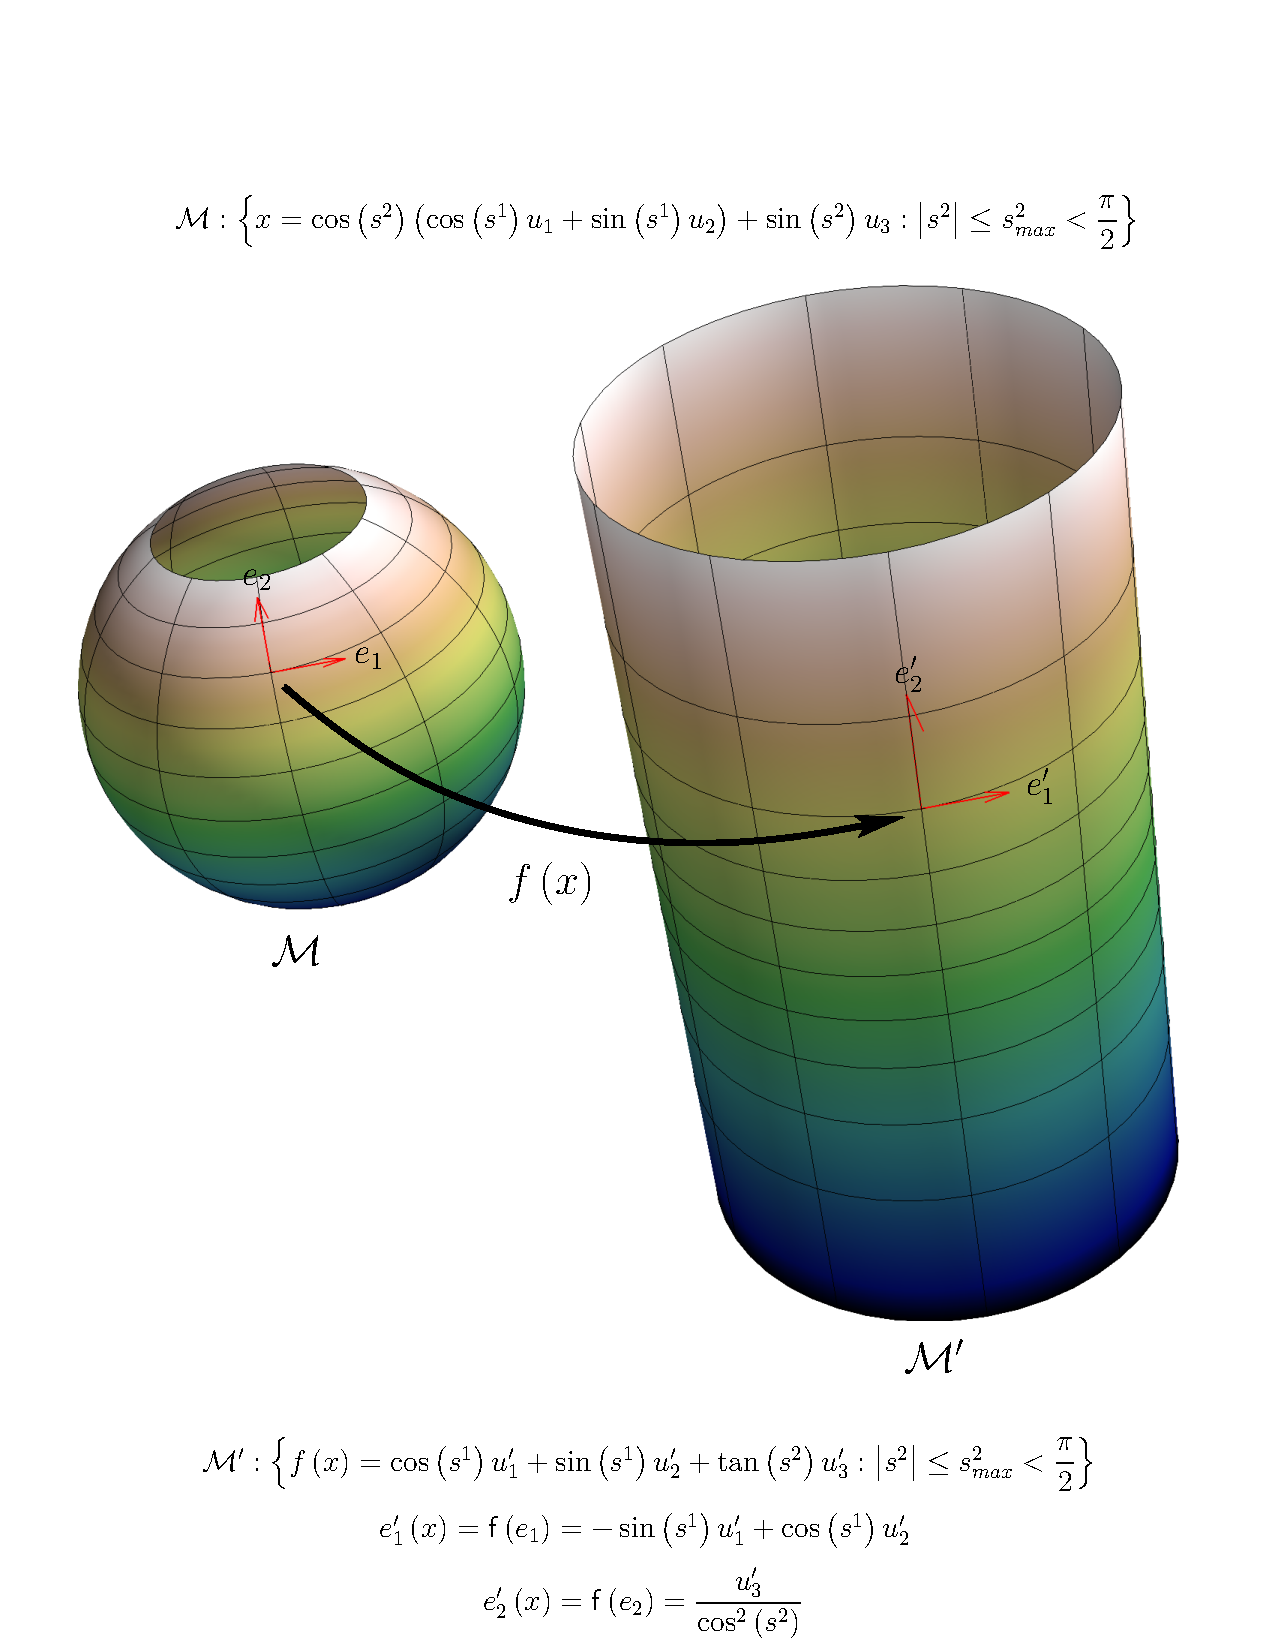
\includegraphics{mercator_annotated.pdf}}
\caption{Mercator mapping of sphere to cylinder manifold. Top and bottom of sphere excluded.}\label{mercator}
\end{center}
\end{figure} 

The cotangent frame, $e^{i}$, in $\mathcal{M}$ is mapped to $e'^{i}$ in $\mathcal{M}'$
via the adjoint of the inverse
\be
e'^{i} = \f{\overline{\sff^{-1}}}{e^{i}}.
\ee
This is simply proved by noting (remember that by definition $a\cdot\f{\bar{\sff}}{b} = b\cdot\f{\sff}{a}$)
\begin{align}
	e'_{i}\cdot e'^{j} &= \f{\sff}{e_{i}}\cdot\f{\overline{\sff^{-1}}}{e^{j}} \nonumber \\
	                   &= e^{j}\cdot\f{\sff^{-1}}{\f{\sff}{e_{i}}} \nonumber \\
                       &= e^{j}\cdot e_{i} \nonumber \\
                       &= \delta_{i}^{j}
\end{align}
The exterior product of two tangent vectors, $e_{i}\W e_{j}$, maps to
\be
	e_{i}\W e_{j} \mapsto  e'_{i}\W e'_{j} = \f{\sff}{e_{i}\W e_{j}}
\ee
since $\sff$ is linear in tangent space arguments.  Likewise if $I'$ is the ``unit" pseudoscalar for the tangent 
space of $\mathcal{M'}$ at $\f{f}{x}$ 
($I'^{2}=\pm 1$) and $I$ the ``unit" pseudoscalar for the tangent space of $\mathcal{M}$ at $x$ ($I^{2}=\pm 1$) then
\be\label{5_102}
	 \f{\sff}{I} = \f{\det}{\sff}I'.
\ee
Since $\sff$ is invertible (the tangent space and its image are isomorphic) we can apply the definition of determinant in 
equation~\ref{1_79} to equation~\ref{5_102}.  For cotangent vectors $e^{i}$ and $e^{j}$
\be
	e'^{i}\W e'^{j} \mapsto \f{\overline{\sff^{-1}}}{e^{i}}\W\f{\overline{\sff^{-1}}}{e^{j}} = \f{\overline{\sff^{-1}}}{e^{i}\W e^{j}}. 
\ee
Since the derivative of a scalar field, $\phi$, is a cotangent vector $\partial\phi = e^{i}\partial_{i}\phi$ and 
$\f{\phi}{x} = \f{\phi'}{x'}$ we can write
\be
	\partial' = \f{\overline{\sff^{-1}}}{\partial} = \f{\overline{\sff^{-1}}}{e^{i}\partial_{i}} = e'^{i}\partial_{i}.
\ee
Since $D$ is also a cotangent vector we also have
\be
	D' = \f{\overline{\sff^{-1}}}{D}.
\ee
For the directional derivative of a scalar field
\begin{align}
	\paren{a'\cdot\partial'}\phi' &= \paren{\f{\sff}{a}\cdot\f{\overline{\sff^{-1}}}{\dot{\partial}}}\dot{\phi} \nonumber \\
	                      &= \paren{\dot{\partial}\cdot\f{\sff^{-1}}{\f{\sff}{a}}}\dot{\phi} \nonumber \\
	                      &= \paren{\dot{\partial}\cdot a}\dot{\phi} \nonumber \\
	                      &= \paren{a\cdot\partial}\phi \label{eq5_106}
\end{align}
or for a vector field 
\be\label{eq5_107}
 \paren{a'\cdot\partial'}b' = \paren{a\cdot\partial}\f{\sff}{b}
\ee
The covariant derivative is constructed using the projection operator, $\prj$, which contains a contraction with the
pseudoscalar $I$.  Thus the covariant derivative depends upon the metric encoded by $\f{I}{x}$.

Consider the following operation where $a$ and $b$ are tangent vectors (from now on the parenthesis around the dot operands are implied) and
using equations~\ref{eq387} and \ref{eq5_45} we get
\begin{align}
	a\cdot\partial b - b\cdot\partial a &= a\cdot D b - b\cdot D a - a\cdot\f{S}{b} + b\cdot\f{S}{a} \nonumber \\
	                                    &= a\cdot D b - b\cdot D a 
\end{align}
since $a\cdot\f{S}{b} = b\cdot\f{S}{a}$ by equation~\ref{eq5_51}. Now define the Lie derivative of $a$ with respect to $b$ by
\be
	\Lie{a}{b} \equiv a\cdot\partial b - b\cdot\partial a
\ee
We will show that
\be
 \Lie{a}{b} \mapsto \Liep{a}{b} = \f{\sff}{\Lie{a}{b}}.
\ee
First note that
\be
	\paren{a\cdot\partial}\f{\sff}{b} - \paren{b\cdot\partial}\f{\sff}{a} = \f{\sff}{\paren{a\cdot\partial}b-\paren{b\cdot\partial}a}
	                                                     +\paren{a\cdot\dot{\partial}}\f{\dot{\sff}}{b}
	                                                     -\paren{b\cdot\dot{\partial}}\f{\dot{\sff}}{a}
\ee
Note that since $\f{\sff}{a}$ is the differential of $\f{f}{x}$ we have ($\partial_{i}e_{j}-\partial_{j}e_{i}=0$)
\begin{align}\label{eq5_112}
	0 = \paren{\partial_{i}\partial_{j}-\partial_{j}\partial_{i}}\f{f}{x} &= \partial_{i}\f{\sff}{e_{j}}-\partial_{j}\f{\sff}{e_{i}} \nonumber \\
																	 0 &= \dot{\partial}_{i}\f{\dot{\sff}}{e_{j}}-\dot{\partial}_{j}\f{\dot{\sff}}{e_{i}}
																	     + \f{\sff}{\partial_{i}e_{j}-\partial_{j}e_{i}}\nonumber \\
																	 0 &= \partial_{i}e'_{j}-\partial_{j}e'_{i}
\end{align}
so that $\partial_{i}e'_{j}-\partial_{j}e'_{i} = 0$ and $\dot{\partial}_{i}\f{\dot{\sff}}{e_{j}}-\dot{\partial}_{j}\f{\dot{\sff}}{e_{i}} = 0$.  Thus
\begin{align}
	\paren{a\cdot\dot{\partial}}\f{\dot{\sff}}{b}-\paren{b\cdot\dot{\partial}}\f{\dot{\sff}}{a} &= 
		\paren{a^{k}e_{k}\cdot e^{i}\dot{\partial}_{i}}\f{\dot{\sff}}{b^{j}e_{j}}
	   -\paren{b^{k}e_{k}\cdot e^{j}\dot{\partial}_{j}}\f{\dot{\sff}}{a^{i}e_{i}} \nonumber \\
	&= a^{i}\dot{\partial}_{i}\f{\dot{\sff}}{b^{j}e_{j}}-b^{j}\dot{\partial}_{j}\f{\dot{\sff}}{a^{i}e_{i}} \nonumber \\
	&= a^{i}b^{j}\dot{\partial}_{i}\f{\dot{\sff}}{e_{j}}-b^{j}a^{i}\dot{\partial}_{j}\f{\dot{\sff}}{e_{i}} \nonumber \\
	&= a^{i}b^{j}\paren{\dot{\partial}_{i}\f{\dot{\sff}}{e_{j}}-\dot{\partial}_{j}\f{\dot{\sff}}{e_{i}}} = 0
\end{align}
and
\be\label{eq5_113}
\paren{a\cdot\partial}\f{\sff}{b} - \paren{b\cdot\partial}\f{\sff}{a} = \f{\sff}{\paren{a\cdot\partial}b-\paren{b\cdot\partial}a}
\ee
and by equations~\ref{eq5_107} and \ref{eq5_113} we have
\be
 \Liep{a}{b} = \f{\sff}{\Lie{a}{b}}
\ee
and the Lie derivative maps simply under $\sff$.

Since $e'^{k}\cdot e'_{j} = \delta_{j}^{k}$ and $e'^{k}\cdot e'_{i} = \delta_{i}^{k}$ we have (using equation~\ref{eq5_112})
\begin{align}\label{eq5_114}
	\partial_{i}\paren{e'^{k}\cdot e'_{j}}-\partial_{j}\paren{e'^{k}\cdot e'_{i}} &= 0 \nonumber \\
	e'^{k}\cdot\paren{\partial_{i}e'_{j}-\partial_{j}e'_{i}}+e'_{j}\cdot\partial_{i}e'^{k}-e'_{i}\cdot\partial_{j}e'^{k} &= 0 \nonumber \\
	e'_{j}\cdot\partial_{i}e'^{k}-e'_{i}\cdot\partial_{j}e'^{k} &= 0 \nonumber \\
	\f{\sff}{e_{j}}\cdot\partial_{i}\f{\overline{\sff^{-1}}}{e^{k}}-\f{\sff}{e_{i}}\cdot\partial_{j}\f{\overline{\sff^{-1}}}{e^{k}} &= 0
\end{align}
Equation~\ref{eq5_114} inplies that $\Prjprm{\f{\overline{\sff^{-1}}}{\partial}\W\f{\overline{\sff^{-1}}}{e^{k}}}=0$ as can be shown by expanding
\begin{align}\label{eq5_115}
	\f{\overline{\sff^{-1}}}{\partial}\W\f{\overline{\sff^{-1}}}{e^{k}} &= \f{\overline{\sff^{-1}}}{e^{i}\partial_{i}}\W\f{\overline{\sff^{-1}}}{e^{k}} \nonumber \\
															  &= e'^{i}\partial_{i}\W e'^{k}
\end{align}
Since equation~\ref{eq5_115} is a grade two multivector we can expand it in terms of the blades (components) $e'^{l}\W e'^{m}$ as follows from
equations~\ref{eq1_75}, \ref{eq1_76}, \ref{eq465}, and the fact that $\partial_{i}$ is a scalar operator that commutes with $\W$.
\begin{align}\label{eq5_116}
	\f{\overline{\sff^{-1}}}{\partial}\W\f{\overline{\sff^{-1}}}{e^{k}} &= e'^{i}\partial_{i}\W e'^{k} \nonumber \\
	\Prjprm{\f{\overline{\sff^{-1}}}{\partial}\W\f{\overline{\sff^{-1}}}{e^{k}}} &= \paren{\paren{e'_{m}\W e'_{l}}\cdot\paren{e'^{i}\partial_{i}\W e'^{k}}}\paren{e'^{l}\W e'^{m}} \nonumber \\
															  &= \paren{\paren{e'_{m}\W e'_{l}}\cdot\paren{e'^{i}\W \partial_{i}e'^{k}}}\paren{e'^{l}\W e'^{m}} \nonumber \\
															  &= \paren{\paren{e'_{m}\cdot\partial_{i}e'^{k}}\paren{e'_{l}\cdot e'^{i}}}-
															     \paren{\paren{e'_{m}\cdot e'^{i}}\paren{e'_{l}\cdot \partial_{i}e'^{k}}}\paren{e'^{l}\W e'^{m}} \nonumber \\
															  &= \paren{\delta_{l}^{i}\paren{e'_{m}\cdot\partial_{i}e'^{k}}-
															     \delta_{m}^{i}\paren{e'_{l}\cdot \partial_{i}e'^{k}}}\paren{e'^{l}\W e'^{m}}  \nonumber \\
															  &= \paren{\paren{e'_{m}\cdot\partial_{l}e'^{k}}-\paren{e'_{l}\cdot \partial_{m}e'^{k}}}\paren{e'^{l}\W e'^{m}}
\end{align}
But the coefficient of $e'^{l}\W e'^{m}$ is the same as equation~\ref{eq5_114} so that $\Prjprm{\f{\overline{\sff^{-1}}}{\partial}\W\f{\overline{\sff^{-1}}}{e^{k}}}=0$.  Note
that since we expanded $\f{\overline{\sff^{-1}}}{\partial}\W\f{\overline{\sff^{-1}}}{e^{k}}$ in terms of $e'^{l}\W e'^{m}$ (cotangent vectors in $\mathcal{M}'$) it was automatically projected into the tangent space of
$\mathcal{M}'$ at $x' = \f{f}{x}$.

Since $D' = \Prjprm{\f{\overline{\sff^{-1}}}{\partial}}$ we have
\be
	D'\W e'^{k} = D'\W\f{\overline{\sff^{-1}}}{e^{k}} = 0.
\ee
and using the product rule the exterior derivative of a blade formed from cotangent vectors is
(just move the term in the product being differentiated to the front using the alternating property
of the ``$\W$'' product)
\be\label{eq5_125}
	D'\W \paren{e'^{k_{1}}\W\dots\W e'^{k_{r}}} = 0.
\ee
Now expand a grade-$r$ multivector field $\f{A}{x}$ on $\mathcal{M}$ in terms of the cotangent vectors
\be
	\f{A}{x} = \f{A_{i_{1}i_{2}\dots i_{r}}}{x}e^{i_{1}}\W e^{i_{2}}\W\dots\W e^{i_{r}}
\ee
Then
\be
	D\W\f{A}{x} = \paren{D\f{A_{i_{1}i_{2}\dots i_{r}}}{x}}\W e^{i_{1}}\W e^{i_{2}}\W\dots\W e^{i_{r}}
\ee
since the exterior derivate of a scalar field is the same as the covariant derivative and that the exterior
derivative of a basis blade is zero. Likewise
\be
	D'\W\f{A'}{x} = \paren{D'\f{A_{i_{1}i_{2}\dots i_{r}}}{x}}\W e'^{i_{1}}\W e'^{i_{2}}\W\dots\W e'^{i_{r}}
\ee
so that for a general multivector field $\f{A}{x}$ on $\mathcal{M}$ we have
\be
	D\W A \mapsto D'\W A' = \f{\overline{\sff^{-1}}}{D\W A}.
\ee
\section{The Fundmental Theorem of Geometric Calculus on Manifolds}
The fundamental theorem of geometric calculus is simply implemented on manifolds.  In figure~\ref{fig5_2} a 
simplicial decomposition of a surface defined by a close curve on a spherical manifold is shown.
\begin{figure}[htbp]
\begin{center}
\scalebox{0.2}{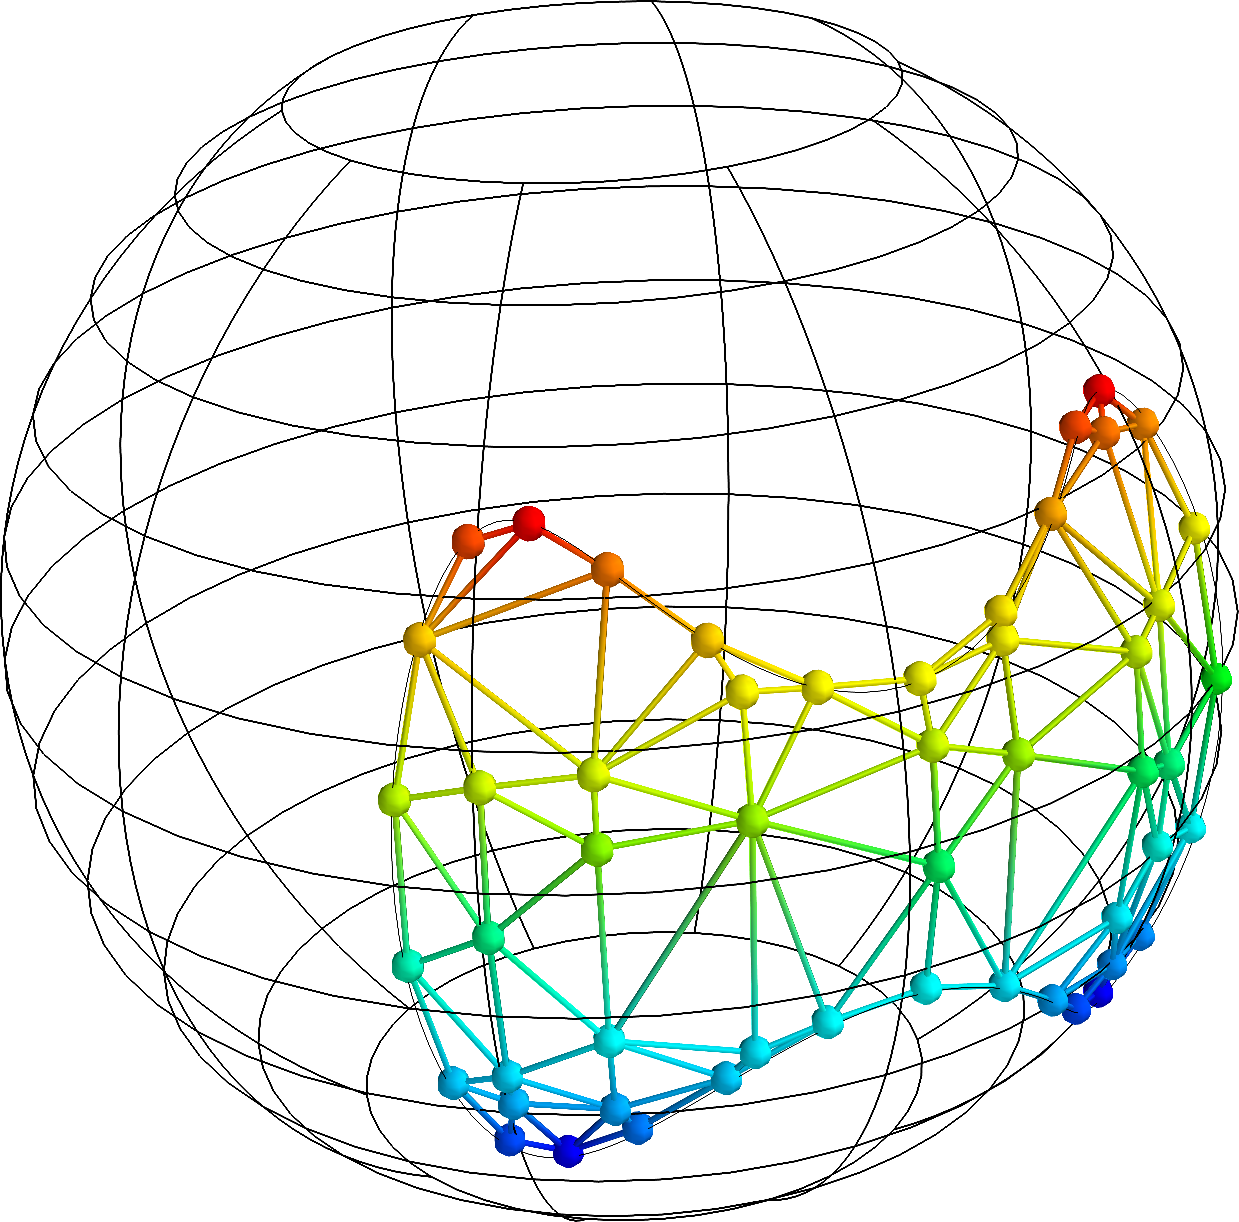
\includegraphics{manifold_simplex.png}}
\caption{Simplical decomposition for surface defined by closed curve on spherical manifold.}\label{fig5_2}
\end{center}
\end{figure} 
The only difference between the derivation of the fundamental theorem of geometical calculus on a vector space 
(which we have proved) and on a manifold is that the pseudo-scalar is not a constant but is now a function of 
position, $\f{I}{x}$, on the manifold.  If we are not on a manifold the pseudo scalars corresponding to the 
oriented volume of each simplex are proportional to one another (they are equal when normalized) so have the
same orientation.  For a manifold the orientation of $\f{I}{x}$ can change with the position vector $x$.  
In the case of figure~\ref{fig5_2} $\f{I}{x}$ is a bi-vector defined by
the tangent space (tangent plane) for each point on the sphere.

Now consider the directed volume element (in the case of figure~\ref{fig5_2} an area element) for each simplex in
figure~\ref{fig5_2} given by $\Delta X = \bfrac{1}{k!}e_{1}\W\dots\W e_{k}$ ($k=2$ for figure~\ref{fig5_2}).  As
the volume (area) of $\Delta X\rightarrow 0$, $\Delta X \propto \f{I}{x}$.

In equation~\ref{eq279} where on the l.h.s. of the equation we are integrating over the boundary of the simplex where
$f$ is a linear approximation to an arbitrary multivector function.
\be
 \oint_{\f{\partial}{x}_{\f{}{k}}}\hspace{-15pt}\f{f}{x} = \dot{f}\dot{\nabla}\cdot\f{}{\Delta X} \nonumber
\ee
consider the operator $\dot{\nabla}\cdot\f{}{\Delta X}$ where we have left the dot on the $\nabla$ to emphasize that it is not
differentiating the $\Delta X$. On a given simplex
\be
	\nabla = e^{i}\pdiff{}{\lambda^{i}}
\ee
where the $\lambda^{i}$'s are the simplical coordinates (equation~\ref{eq237}) and the $e^{i}$'s are the reciprocal vectors to the $e_{i}$'s that
define the simplex.  In the case of a manifold as the volume of $\Delta X \rightarrow 0$ the $e_{i}$'s (since the $e^{i}$'s
define the same subspace as the $e_{i}$'s) define a pseudoscalar that is proportional to $\f{I}{x}$ so that $e^{i}\pdiff{}{\lambda^{i}}$
is the projection of the geometric derivative, $\nabla$, from the embedding vector space of the manifold to the tangent space
of the manifold at point $x$.  Thus in the case of a manifold as the volume of $\Delta X \rightarrow 0$ we have 
$\partial = e^{i}\pdiff{}{\lambda^{i}}$.

Note that
\be
	\dot{\partial}\f{}{\Delta X} = \dot{\partial}\cdot\f{}{\Delta X}+\dot{\partial}\W\f{}{\Delta X}
\ee
but $\dot{\partial}\W\f{}{\Delta X} = 0$ since $\partial$ is within the subspace (tangent space) defined by $\Delta X$.  The
fundamental theorem of geometric calculus as applied to a manifold is
\be\label{eq5_127}
	\oint_{\partial V}\f{\Llin}{dS} =  \int_{V}\f{\dot{\Llin}}{\dot{\nabla}\cdot dX} = \int_{V}\f{\dot{\Llin}}{\dot{\partial}dX}
\ee
One can write $dX = \f{I}{x}\abs{dX}$ and note that $\partial$ or $\nabla$ in equation~\ref{eq5_127} do not differentiate $\f{I}{x}$.
\subsection{Divergence Theorem on Manifolds}
Let $\f{\Llin}{A} = \grade{JAI^{-1}}{}$ where $J$ is a vector field in the tangent space of the manifold and substitute into
equation~\ref{eq5_127} to get
\be\label{eq5_128}
 \oint_{\partial V}\grade{J dS I^{-1}}{} = \int_{V}\paren{\grade{\dot{J}\dot{\partial}dXI^{-1}}{}+\grade{J\dot{\partial}dX\dot{I^{-1}}}{}}.
\ee
Now reduce equation~\ref{eq5_128} by noting that $ndS = I\abs{dS}$ where $n$ is the outward normal to the surface element $dS$. We can define
an outward normal in $n$-dimensional manifold since the grade of $dS$ is $n-1$ and it defines a subspace of the tangent space of dimension $n-1$
for which a unique normal exists. This gives
\begin{align}
dS &= \bfrac{n}{n^{2}}I\abs{dS} \\
\grade{J dS I^{-1}}{} &= \bfrac{\abs{dS}}{n^{2}}\grade{JnII^{-1}}{} \nonumber \\
                      &= \bfrac{\abs{dS}}{n^{2}}\grade{Jn}{} \nonumber \\
                      &= \bfrac{J\cdot n\abs{dS}}{n^{2}} 
\end{align}
Also
\begin{align}
\dot{J}\dot{\partial}dXI^{-1} &= \dot{J}\dot{\partial}I\abs{dX}I^{-1} \nonumber \\
                              &= \dot{J}\dot{\partial}\abs{dX} \\
\grade{\dot{J}\dot{\partial}dXI^{-1}}{} &= \grade{\dot{J}\dot{\partial}\abs{dX}}{} \nonumber \\
                                        &= \grade{\dot{J}\dot{\partial}}{}\abs{dX} \nonumber \\
                                        &= \partial\cdot J\abs{dX}.
\end{align}
Finally, since both $I^{-1}$ and $dX$ are proportional to $I$
\begin{align}
\grade{J\dot{\partial}\dot{I^{-1}}dX}{} &= \pm\grade{J\dot{\partial}\dot{I}I}{}\abs{dX} \nonumber \\
                                        &= \pm\bfrac{1}{2}\grade{J\dot{\partial}\f{}{\dot{I}I+I\dot{I}}}{}\abs{dX} \nonumber \\
                                        &= \pm\bfrac{1}{2}\grade{J\partial\f{}{I^{2}}}{}\abs{dX} \nonumber \\
                                        &= 0
\end{align}
so that the divergence theorem is 
\be
 \oint_{\partial V}\bfrac{n}{n^{2}}\cdot J \abs{dS} = \int_{V}\partial\cdot J\abs{dX}
\ee
\subsection{Stokes Theorem on Manifolds}
Assume that the manifold tangent space dimension is $s+1$ and $B_{r}$ is a grade $r$ multivector field.  For clarity we denote
the grade of volume and surface elements with a subscript on the $d$'s so that $dX = d_{s+1}X$ and $dS = d_{s}S$.  Now let
$\f{\Llin}{A} = \grade{B_{r}A}{\abs{s-r}}$ so that the application of equation~\ref{eq5_127} gives
\begin{align}\label{eq5_135}
	\oint_{\partial V}\grade{B_{r}d_{s}S}{\abs{s-r}} &= \int_{V}\grade{\dot{B}_{r}{\dot{\partial}}d_{s+1}X}{\abs{s-r}} \nonumber \\
	\oint_{\partial V}\overbrace{B_{r}\cdot d_{s}S}^{\mbox{grade $\abs{s-r}$}} &= \int_{V}\grade{\f{}{\overbrace{\dot{B}_{r}\W\dot{\partial}}^{\mbox{grade $r+1$}}+
	                                       \underbrace{\dot{B}_{r}\cdot\dot{\partial}}_{\mbox{grade $r-1$}}}d_{s+1}X}{\abs{s-r}} \nonumber \\
                                            &= \paren{-1}^{r}\int_{V}\grade{\underbrace{\paren{\partial\W B_{r}}d_{s+1}X}_{\mbox{lowest grade is $\abs{s-r}$}}}{\abs{s-r}}
                                               +\int_{V}\grade{\underbrace{\paren{\dot{B}_{r}\cdot\dot{\partial}}d_{s+1}X}_{\mbox{lowest grade is $\abs{s-r+2}$}}}{\abs{s-r}} \nonumber \\
                                            &= \paren{-1}^{r}\int_{V}\paren{\partial\W B_{r}}\cdot d_{s+1}X
\end{align}
However 
\be
 	\paren{\partial\W B_{r}}\cdot d_{s+1}X = \paren{D\W B_{r}}\cdot d_{s+1}X  
\ee
since $d_{s+1}X = \f{I_{s+1}}{x}\abs{d_{s+1}X}$ and the dot product of any component of $\partial\W B_{r}$ that is not in the tangent space defined by $\f{I_{s+1}}{x}$ is zero so that
\be\label{eq5_137}
	\oint_{\partial V}B_{r}\cdot d_{s}S = \int_{V}\paren{\dot{B}_{r}\W\dot{D}}\cdot d_{s+1}X = \paren{-1}^{r}\int_{V}\paren{D\W B_{r}}\cdot d_{s+1}X
\ee
The divergence theorem is recovered when $r=s-1$.  This is important for constructing conservation theorems in curved spaces. Equation~\ref{eq5_137} is the most
general application of equation~\ref{eq5_127} that allows one to replace $\partial$ with $D$ (covariant derivative) on a manifold.

\section{Differential Forms in Geometric Calculus}
\subsection{Inner Products of Subspaces}\label{sect5_6_1}
Start by considering products of the form where $A_{r}$ and $B_{r}$ are $r$-grade blades
\be
 A^{\R}_{r}\cdot B_{r} = \paren{a_{1}\W\dots\W a_{r}}^{\R}\cdot\paren{b_{1}\W\dots\W b_{r}}
\ee
Both $A_{r}$ and $B_{r}$ define $r$-dimensional subspaces of the vector space via the equations $x\W A_{r} = 0$ and $x\W B_{r} = 0$.  
We show that if $A_{r}$ and $B_{r}$ do not 
define the same subspace then $A^{\R}_{r}\cdot B_{r} = 0$. Assume that they do not define the same subspaces, but
that the intersection of the subspaces has dimension $s<r$ so that one can have an orthogonal basis for $A_{r}$ of
$\Set{e_{1},\dots,e_{s},e_{s+1},\dots,e_{r}}$ and an orthogonal basis for $B_{r}$ of $\Set{e_{1},\dots,e_{s},e'_{s+1},\dots,e'_{r}}$. 
Then the geometric product of $A^{\R}_{r}$ and $B_{r}$ is
\begin{align}
 A^{\R}_{r}B_{r} &= \alpha e_{r}\dots e_{s+1}e_{s}\dots e_{1}\beta e_{1}\dots e_{s}e'_{s+1}\dots e'_{r} \nonumber \\
            &= \paren{\alpha\beta e_{1}^{2}\dots e_{s}^{2}}e_{s+1}\dots e_{1}e'_{s+1}\dots e'_{r}
\end{align}
where the quantity in parenthesis is a scalar and the other factors a blade of grade $2\paren{r-s}$. Thus 
\be\label{eq5_145}
	A^{\R}_{r}\cdot B_{r} = \braket{A^{\R}_{r}B_{r}} = 0.
\ee
If $A_{r}$ and $B_{r}$ define the same $r$-dimensional subspace let $\Set{e_{1},\dots, e_{r}}$ be an orthogonal basis for the subspace and
expand $A_{r}$ and $B_{r}$ in terms of the orthogonal basis vectors and reciprocal orthogonal basis vectors respectively -
\be\label{eq5_141}
	a_{i} = \paren{a_{i}\cdot e^{j}}e_{j}
\ee
and 
\be\label{eq5_142}
	b_{i} = \paren{b_{i}\cdot e_{j}}e^{j}
\ee
Let the matrices of the coefficients in equations~\ref{eq5_141} and \ref{eq5_142} be denoted by $\Mat{a_{i}\cdot e^{j}}$ and 
$\Mat{b_{i}\cdot e_{j}}$.  Then we can expand $A_{r}$ and $B_{r}$ as
\be
	A_{r} = \det\paren{\Mat{a_{i}\cdot e^{j}}}e_{1}\dots e_{r}
\ee
and
\be
	B_{r} = \det\paren{\Mat{b_{i}\cdot e_{j}}}e^{1}\dots e^{r}
\ee
and (since the determinant of a matrix and determinant of the transpose of matrix are equal)
\begin{align}
A^{\R}_{r}\cdot B_{r} &= \det\paren{\Mat{a_{i}\cdot e^{j}}}\det\paren{\Mat{b_{i}\cdot e_{j}}}\braket{e_{r}\dots e_{1}e^{1}\dots e^{r}} \nonumber \\
                      &= \det\paren{\Mat{a_{i}\cdot e^{j}}}\det\paren{\Mat{b_{i}\cdot e_{j}}} \nonumber \\
                      &= \det\paren{\Mat{a_{i}\cdot e^{j}}}\det\paren{\Mat{b_{i}\cdot e_{j}}^{T}} \nonumber \\
                      &= \det\paren{\Mat{a_{i}\cdot e^{j}}}\det\paren{\Mat{b_{j}\cdot e_{i}}} \nonumber \\
                      &= \det\paren{\Mat{\paren{a_{i}\cdot e^{k}}\paren{b_{j}\cdot e_{k}}}}
\end{align}
But 
\begin{align}
 a_{i}\cdot b_{j} &= \paren{a_{i}\cdot e^{k}}e_{k}\cdot\paren{b_{j}\cdot e_{l}}e^{l} \nonumber \\
                  &= \paren{a_{i}\cdot e^{k}}\paren{b_{j}\cdot e_{l}}\delta^{l}_{k} \nonumber \\
                  &= \paren{a_{i}\cdot e^{k}}\paren{b_{j}\cdot e_{k}}
\end{align}
So that
\be
A^{\R}_{r}\cdot B_{r} = \det\paren{\Mat{a_{i}\cdot b_{j}}}.
\ee
From our derivations we see that if $A_{r}$ is a general $r$-grade multivector (not a blade) we can always find a $r$-grade blade such that
\be
	A^{\R}_{r}\cdot\paren{b_{1}\W\dots\W b_{r}} = \paren{a_{1}\W\dots\W a_{r}}^{\R}\cdot\paren{b_{1}\W\dots\W b_{r}}.
\ee
Now consider the relation between the basis $\Set{a_{1},\dots, a_{n}}$ and the reciprocal basis $\Set{a^{1},\dots, a^{n}}$ for an $n$-dimensional vector space where 
in equation~\ref{eq5_149} $r \le n$ and $1 \le i_{l},j_{m} \le n$
\be\label{eq5_149}
	\paren{a_{i_{1}}\W\dots\W a_{i_{r}}}^{\R}\cdot\paren{a^{j_{1}}\W\dots\W a^{j_{r}}} = \det\paren{\Mat{a_{i_{l}}\cdot a^{j_{m}}}} = \det\paren{\Mat{\delta_{i_{l}}^{j_{m}}}}
\ee
where $i_{1}<i_{2}<\dots<i_{r}$ and  $j_{1}<j_{2}<\dots<j_{r}$.  Equation~\ref{eq5_149} is zero unless $i_{l}=j_{l}$ for all $1\le l \le r$ so that
\be
    \paren{a_{i_{1}}\W\dots\W a_{i_{r}}}^{\R}\cdot\paren{a^{j_{1}}\W\dots\W a^{j_{r}}} = \delta_{i_{1}}^{j_{1}}\delta_{i_{2}}^{j_{2}}\dots\delta_{i_{r}}^{j_{r}}.
\ee
since if the index ordering condition is satisfied for the $i_{l}$'s and the $j_{m}$'s and there is an index, $l$, such that $i_{l} \ne j_{l}$ then the two blades do not
define the same subspace and the inner product is zero.  The square of a blade is given by
\begin{align}
	\paren{a_{1}\W\dots\W a_{r}}^{2} &= \paren{a_{1}\W\dots\W a_{r}}\cdot\paren{a_{1}\W\dots\W a_{r}} \\
	                               &= \paren{-1}^{\frac{r(r-1)}{2}}\paren{a_{1}\W\dots\W a_{r}}^{\R}\cdot\paren{a_{1}\W\dots\W a_{r}} \\
	                               &= \paren{-1}^{\frac{r(r-1)}{2}}\f{\det}{\Mat{a_{i}\cdot a_{j}}} \label{eq5_158}\\
	                               &= \paren{-1}^{\frac{r(r-1)}{2}}a_{1}^{2}\dots a_{r}^{2} \mbox{ if the $a_{i}$'s are orthogonal}.
\end{align}

\subsection{Alternating Forms}
If $V$ is a vector space then an $r$-rank tensor is a multilinear map
\be
	\f{T_{r}}{v_{1},\dots,v_{r}}:\bigotimes\limits_{i=1}^{r}V\rightarrow\mathcal{R}
\ee
where ($\otimes$ is the cartesian product of vector spaces)
\be
	\bigotimes\limits_{i=1}^{r}V = \underbrace{V\otimes\dots\otimes V}_{\mbox{$r$ times}}
\ee
so that if $v_{i}\in V$ the tuple $\paren{v_{1},\dots,v_{r}}\in \bigotimes\limits_{i=1}^{r}V$.

The sum of two $r$-rank tensors is the $r$-rank tensor defined by
\be
	\f{\paren{A_{r}+B_{r}}}{v_{1},\dots,v_{r}} \equiv \f{A_{r}}{v_{1},\dots,v_{r}}+\f{B_{r}}{v_{1},\dots,v_{r}}.
\ee
The tensor product of rank $r$ and $s$ tensors is a rank $r+s$ tensor defined by
\be
	\f{\paren{A_{r}\otimes B_{s}}}{v_{1},\dots,v_{r+s}} \equiv \f{A_{r}}{v_{1},\dots,v_{r}}\f{B_{s}}{v_{r+1},\dots,v_{r+s}}.
\ee
An $r$-form (when we say something is a form from now on we mean alternating form) is an $r$-rank tensor with the property (no summation in this case)
\be
\f{\alpha_{r}}{v_{1},\dots,v_{r}} = \epsilon^{i_{1}\dots i_{r}}_{1\dots r}\f{\alpha_{r}}{v_{i_{1}},\dots,v_{i_{r}}}
\ee
where $\epsilon^{i_{1}\dots i_{r}}_{1\dots r}$ is the mixed rank permutation symbol.  We can always construct an $r$-form from an $r$-rank tensor via 
\be
	\f{\alpha_{r}}{v_{1},\dots,v_{r}} = \f{\epsilon}{A_{r}} \equiv \sum_{i_{1},\dots,i_{r}}\epsilon_{i_{1}\dots i_{r}}^{1\dots r}\f{A_{r}}{v_{i_{1}},\dots,v_{i_{r}}}
\ee
In the geometric algebra a simple representation of an alternating $r$-form is
\be
	\f{\alpha_{r}}{v_{1},\dots,v_{r}} = A^{\R}_{r}\cdot\paren{v_{1}\W\dots\W v_{r}}
\ee
where $A_{r}$ is a grade-$r$ multivector.  Since the grade of $A_{r}$ and the grade of $\paren{v_{1}\W\dots\W v_{r}}$ are the same the 
inner product results in a scalar and also since $\paren{v_{1}\W\dots\W v_{r}}$ is a blade it alternates sign upon exchange of adjacent
vectors.

The basic operations of the ``Algebra of Forms'' inherit the sum and cartesian product operations from tensor since they are tensors.  However, 
in order to construct an algebra of forms we need a product of two forms that results in a form.  The tensor product of two alternating forms is
not an alternating form, but since we know how to convert a tensor to a form we define the exterior product of an $r$-form and $s$-form to be 
the $r+s$ form
\be\label{eq5_158}
	\alpha_{r}\Wbld \beta_{s} \equiv \f{\epsilon}{\alpha_{r}\otimes\beta_{s}}
\ee
as an example
\be
	\f{\alpha_{1}}{v_{1}}\Wbld\f{\beta_{1}}{v_{2}} = \f{\alpha_{1}}{v_{1}}\f{\beta_{1}}{v_{2}}-\f{\alpha_{1}}{v_{2}}\f{\beta_{1}}{v_{1}}
\ee
so that
\be
\f{\alpha_{r}}{v_{1},\dots,v_{r}}\Wbld\f{\beta_{s}}{v_{r+1},\dots,v_{r+s}} = \paren{A_{r}\W B_{s}}^{\R}\cdot\paren{v_{1}\W\dots\W v_{r+s}}
\ee
and
\be
	\alpha_{r}\Wbld\beta_{s} = \paren{-1}^{rs}\beta_{s}\Wbld\alpha_{r}
\ee
The interior product of an $r$ and $s$-form is defined by ($r > s$) an $r-s$ form (note that we are distinguishing the inner, $\cdotbld$, and
exterior, $\Wbld$, products for forms from the geometric algebra products by using boldface symbols)
\be
\beta_{s}\cdotbld\alpha_{r} \equiv \paren{B_{s}\cdot A_{r}}^{\R}\cdot\paren{v_{s+1}\W\dots\W v_{r}}
\ee
A $r$-form is simple if $A_{r}$ is a blade ($A_{r} = a_{1}\W\dots\W a_{r}$).

\subsection{Dual of a Vector Space}
Let $V$ be a $n$-dimensional vector space.  The set of all linear maps $f:V\rightarrow \mathcal{R}$ is denoted $V^{*}$ and is a vector space called the
dual space of $V$. $V^{*}$ is a $n$-dimensional vector space since for $f,g:V\rightarrow \mathcal{R}$, $x \in V$, $\alpha \in \mathcal{R}$ and we define
\begin{align}
	\f{\paren{f+g}}{x} \equiv \f{f}{x} +\f{g}{x} \\
	\f{\paren{\alpha f}}{x} \equiv \alpha\f{f}{x} \\
	\f{0}{x} \equiv 0
\end{align}
Then by the linearity of $\f{f}{x}$ and $\f{g}{x}$, $\f{\paren{f+g}}{x}$, $\f{\alpha f}{x}$, and $\f{0}{x}$ are also linear functions of $x$ and $V^{*}$ is
a vector space.

Let $\mathbf{e}_{i}$ be a basis for $V$ and define $\sigma^{i} \in V^{*}$ by
\be
	\f{\sigma^{i}}{\mathbf{e}_{j}} = \delta_{j}^{i}
\ee
so that if $x = x^{i}\mathbf{e}_{i} \in V$ then
\be
	\f{\sigma^{i}}{x} =  \f{\sigma^{i}}{x^{j}\mathbf{e}_{j}} = x^{i} 
\ee
so that for any $f \in V^{*}$
\be
	\f{f}{x} = \f{f}{x^{i}\mathbf{e}_{i}} = x^{i}\f{f}{\mathbf{e}_{i}}
\ee
Now assume that
\begin{align}
	0 &= a_{i}\f{\sigma^{i}}{\mathbf{e}_{j}} \\
	  &= a_{i}\delta_{j}^{i} \\
	  &= a_{j} 
\end{align}
so the $\sigma^{i}$ are linearly independent. Now assume $f \in V^{*}$.  Then
\begin{align}
	\f{f}{x} &= \f{f}{x^{i}\mathbf{e}_{i}} \\
	         &= x^{i}\f{f}{\mathbf{e}_{i}} \\
	         &= \f{f}{\mathbf{e}_{i}}\f{\sigma^{i}}{x} \\
	         &= \f{\paren{\f{f}{\mathbf{e}_{i}}\sigma^{i}}}{x}
\end{align}
Thus
\be
	f = \f{f}{\mathbf{e}_{i}}\sigma^{i}
\ee
and the $\sigma^{i}$ form a basis for $V^{*}$.  If the $\mathbf{e}_{i}$ form an 
orthonormal basis for $V$ (remember that orthonomal implies orthogonal and orthogonal
implies that a dot product is defined since the dot product is used to define orthogonal) then
\be
	\f{\sigma^{i}}{x} = \mathbf{e}_{i}\cdot x.
\ee
Since for 1-forms, $\alpha:V\rightarrow\mathcal{R}$, we have $\alpha\in V^{*}$.  The most
general 1-form can be written
\be
	\f{\alpha}{v} = \alpha_{i}\f{\sigma^{i}}{v}.
\ee
If $\alpha$ is a 2-form, $\f{\alpha}{v_{1},v_{2}}$, the bases are $\sigma^{i}\Wbld\sigma^{j}$, and
the most general 2-form is written as
\be
	\f{\alpha}{v_{1},v_{2}} = \sum_{i<j}\alpha_{ij}\f{\sigma^{i}}{v_{1}}\Wbld\f{\sigma^{j}}{v_{2}}	
\ee
since $\sigma^{i}\Wbld\sigma^{i}=0$ and $\sigma^{i}\Wbld\sigma^{j}=-\sigma^{i}\Wbld\sigma^{j}$ from
the definition in equation~\ref{eq5_158}.

\subsection{Standard Definition of a Manifold}
Let $\mathcal{M}^{n}$ be any set\footnote{This section is based upon sections 1.2 and 2.1 in 
``The Geometry of Physics, An Introduction (Second Edition),'' by T. Frankel} that has 
a covering of subsets, $\mathcal{M}^{n} = U\cup V\cup\dots$ such that
\begin{enumerate}
	\item For each subset $U$ there is a one to one mapping $\phi_{U}:U\rightarrow\mathcal{R}^{n}$ where $\f{\phi_{U}}{U}$ is an 
	open subset of $\mathcal{R}^{n}$.
	\item Each $\f{\phi_{U}}{U\cap V}$ is an open subset of $\mathcal{R}^{n}$.
	\item The overlap maps
		\be
			f_{UV}= \phi_{V}\circ\phi_{U}^{-1}: \f{\phi_{U}}{U\cap V}\rightarrow\mathcal{R}^{n}
		\ee
	or equivalently the compound maps
		\be
			\f{\phi_{U}}{U\cap V}\stackrel{\phi_{U}^{-1}}{\longrightarrow}\mathcal{M}^{n}\stackrel{\phi_{V}}{\longrightarrow}\mathcal{R}^{n}
		\ee
	are differentiable.
	\item Take a maximal atlas of coordinate patches $\Set{(U,\phi_{U}),(V,\phi_{V}),\dots}$ and define a topology for $\mathcal{M}^{n}$ by defining
	that a subset $W\subset \mathcal{M}^{n}$ is open if for any $p \in W$ there is a $(U,\phi_{U})$ such that $p\in U\subset W$.
\end{enumerate}
If the resulting topology for $\mathcal{M}^{n}$ is Hausdorff and has a countable base we say $\mathcal{M}^{n}$ is an $n$-dimensional differentiable manifold 
(look it up since I don't know what it means\footnote{G. Simmons,{\em Topology and Modern Analysis}, McGraw-Hill,1963}).

Figure~\ref{fig5_3} (page 94) shows the relationships between the Manifold and the coordinate patch mappings.

\begin{figure}[htbp]
\begin{center}
\scalebox{0.75}{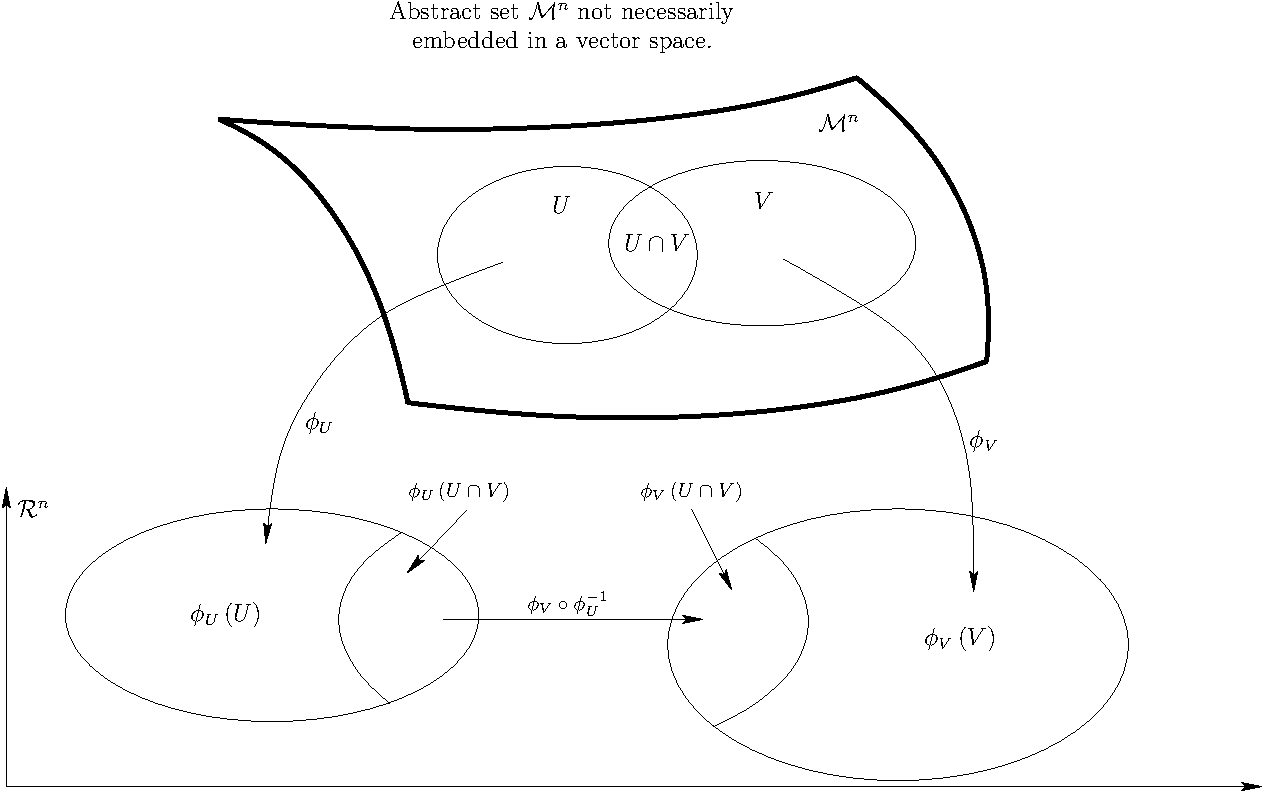
\includegraphics{manifolddef_crop.pdf}}
\caption{Fundamental Manifold Mappings.}\label{fig5_3}
\end{center}
\end{figure}

If $f:\mathcal{M}^{n}\rightarrow\mathcal{R}$ is a real valued function on the manifold $\mathcal{M}^{n}$ it is differentiable if $f_{U} = f\circ\phi_{U}^{-1}$
is differentiable with respect to the coordinates $\Set{x^{1}_{U},\dots, x^{n}_{U}}$ for any coordinate patch $(U,\phi_{U})$.  The real scalars 
$\Set{x^{1}_{U},\dots, x^{n}_{U}}$
(denoted by the tuple $x=\paren{x^{1}_{U},\dots,x^{n}_{U}}$) form a coordinate system for $\f{\phi_{U}}{U} \subset \mathcal{R}^{n}$.  In the future we shall simply
say that $f$ is differentiable if $f_{U}$ is differentiable.  Likewise we will shall usually omit the process of replacing $f$ by its composition 
$f\circ\phi_{U}^{-1}$, thinking of $f$ as directly expressible as a function $\f{f}{x} = \f{f}{x^{1}_{U},\dots,x^{n}_{U}}$ of any local coordinates.

Now let $p \in U\cap V \subset \mathcal{M}^{n}$ and 
\be
	x_{U} = \paren{x_{U}^{1},\dots,x_{U}^{n}} = \f{\phi_{U}}{p}\mbox{ and }x_{V} = \paren{x_{V}^{1},\dots,x_{V}^{n}} = \f{\phi_{V}}{p}. \nonumber
\ee
Then
\be
	x_{U} = \f{\phi_{U}\circ\phi_{V}^{-1}}{x_{V}}=\f{x_{U}}{x_{V}}\mbox{ and } x_{V} = \f{\phi_{V}\circ\phi_{U}^{-1}}{x_{U}}=\f{x_{V}}{x_{U}}. \nonumber
\ee
Let $X_{U} = \paren{X_{U}^{1},\dots,X_{U}^{n}}$ and consider the linear approximation to $\f{\phi_{V}\circ\phi_{U}^{-1}}{x_{U}+hX_{U}}$ where $h$ is a 
small number. Then in the linear approximation
\be
	\f{\phi_{V}\circ\phi_{U}^{-1}}{x_{U}+hX_{U}} = \f{x_{V}}{x_{U}}+h\mat{\pdiff{x_{V}^{i}}{x_{U}^{j}}}X_{U}^{T} = x_{V}+hX_{V}
\ee
so that
\be\label{eq5_161}
	X_{V}^{i} = \pdiff{x_{V}^{i}}{x_{U}^{j}}X_{U}^{j}
\ee
where $\mat{\pdiff{x_{V}^{i}}{x_{U}^{j}}}$ is the Jacobian matrix of the coordinate transformation from one coordinate patch to another and $X_{U}^{T}$ is the 
transpose (colume vector) of the tuple $X_{U}$ (row vector).  
\subsection{Tangent Space}
Now consider the case of a vector manifold in Euclidian space.  The definition of the tangent vector generalizes the concept of the directional derivative
in $\mathcal{R}^{n}$. if $X_{p}$ is a vector at point $p \in \mathcal{R}^{n}$ and $f:\mathcal{R}^{n}\rightarrow\mathcal{R}$ is a $C^{\infty}$ function in
the neighborhood of $p$ then define
\be
	\f{X_{p}}{f} \equiv X_{p}\cdot\Eval{\nabla f}{p}.
\ee
If $f$ and $g$ are $C^{\infty}$ and $\alpha,\beta \in \mathcal{R}$ we have (from the properties of $\cdot$ and $\nabla$)
\begin{align}
	\f{X_{p}}{\alpha f+\beta g} &= \alpha\f{X_{p}}{f} + \beta \f{X_{p}}{g} \\
	\f{X_{p}}{fg} &= \f{f}{p}\f{X_{p}}{g} + \f{g}{p}\f{X_{p}}{f}
\end{align}
Let $\f{C^{\infty}}{p}$ denote the set of real functions that are $C^{\infty}$ on some neighborhood of $p \in \mathcal{M}^{n}$. The generalization 
of the tangent vector to an abstract manifold at a point $p \in \mathcal{M}^{n}$ is defined as a real valued function $X_{p}: \f{C^{\infty}}{p}\rightarrow\mathcal{R}$
such that ($f,g \in \f{C^{\infty}}{p}$ and $\alpha \in \mathcal{R}$)
\begin{align} 
	\f{X_{p}}{f+g} &= \f{X_{p}}{f}+\f{X_{p}}{g} \label{eq5_187}\\
	\f{X_{p}}{\alpha f} &= \alpha\f{X_{p}}{f} \label{eq5_188}\\
	\f{X_{p}}{fg} &= \f{f}{p}\f{X_{p}}{g}+\f{g}{p}\f{X_{p}}{f}.\label{eq5_189}
\end{align}
A tangent vector is often called a derivation on $\f{C^{\infty}}{p}$.  For a given coordinate patch $\paren{U,\phi_{U}}$ we define the tangent space basis
vectors $\paren{\pdiff{}{x^{i}_{U}}}_{p}$ by 
\be\label{eq5_190}
	\Pval{\pdiff{}{x^{i}_{U}}}{p}f \equiv \Eval{\pdiff{\paren{f\circ\phi^{-1}_{U}}}{x^{i}_{U}}}{\f{\phi_{U}}{p}}.
\ee
Since they are partial derivatives the $\Pval{\pdiff{}{x^{i}_{U}}}{p}$ trivially satisfy equations~\ref{eq5_187}, \ref{eq5_188}, and \ref{eq5_189}.  The
general tangent vector is then given by the scalar linear differential operator
\be
	X_{p} = X^{i}_{U}\Pval{\pdiff{}{x^{i}_{U}}}{p}
\ee
Thus we require for $X_{p}$
\be
	\f{X_{p}}{f} = X^{i}_{U}\Pval{\pdiff{}{x^{i}_{U}}}{p}f = X^{j}_{V}\Pval{\pdiff{}{x^{j}_{V}}}{p}f
\ee
for all $p \in U\cap V$.  Thus
\begin{align}
	X^{i}_{U}\Pval{\pdiff{}{x^{i}_{U}}}{p}f &= X^{j}_{V}\Pval{\pdiff{}{x^{j}_{V}}}{p}f \\
	X^{i}_{U}\Pval{\pdiff{x^{k}_{V}}{x^{i}_{U}}}{p}\Pval{\pdiff{}{x^{k}_{V}}}{p}f &= X^{j}_{V}\Pval{\pdiff{}{x^{j}_{V}}}{p}f
\end{align}
and
\be\label{eq5_195}
	X^{j}_{V} = X^{i}_{U}\Pval{\pdiff{x^{j}_{V}}{x^{i}_{U}}}{p}
\ee
is the transformation law for the components, $X^{i}_{U}$, of the tangent vectors.

We have established an isomorphism between the tuple $\paren{X^{1}_{U},\dots,X^{n}_{U}}$ that transforms as in equation~\ref{eq5_161} and the scalar
linear operator $X_{p}$ so that
\be
	\paren{X^{1}_{U},\dots,X^{n}_{U}} \Leftrightarrow X^{i}_{U}\pdiff{}{x^{i}_{u}}
\ee
since 
\be
	X_{U}^{i}\pdiff{f}{x_{U}^{i}} = X_{V}^{j}\pdiff{f}{x_{V}^{i}},\:\:\forall\:f:\mathcal{M}^{n}\rightarrow\mathcal{R}
\ee
implies equation~\ref{eq5_161}.
A vector field on a manifold is then a tangent vector with coefficients, $\f{X^{i}}{p}$ that are functions of the position $p$ on the manifold 
so that ($x_{U} = \paren{x^{1}_{U},\dots,x^{n}_{U}}$) 
\be\label{eq5_205}
	\f{X}{p} = \f{X_{U}}{x_{U}} = \f{X^{i}_{U}}{x_{U}}\Pval{\pdiff{}{x^{i}_{U}}}{p} = \f{X^{i}_{U}}{x^{1}_{U},\dots,x^{n}_{U}}\Pval{\pdiff{}{x^{i}_{U}}}{p}
\ee
and the coefficients $\f{X^{i}_{U}}{x_{U}}$ transform under a change of basis according to equation~\ref{eq5_195}.

\subsection{Differential Forms and the Dual Space}

If $f:\mathcal{M}^{n}\rightarrow\mathcal{R}$ we define the differential of $f$ at $p\in\mathcal{M}^{n}$, $df:\mathcal{M}^{n}_{p}\rightarrow\mathcal{R}$
where $X_{p}\in\mathcal{M}^{n}_{p}$ as the linear functional
\be
	\f{df}{X} \equiv \f{X_{p}}{f}
\ee
so that in general case of $X$ being a vector field (we are supressing the the patch index $U$)
\be
	\f{df}{\f{X}{p}} = \f{df}{\f{X^{i}}{p}\Pval{\pdiff{}{x^{i}}}{p}} = \f{X^{i}}{p}\Eval{\pdiff{f}{x^{i}}}{p}.
\ee
If $\f{f}{p}=\f{x^{i}}{p}$ are the coordinate functions we have
\be
	\f{dx^{i}}{\Pval{\pdiff{}{x^{j}}}{p}} = \Eval{\pdiff{x^{i}}{x^{j}}}{p} = \delta^{i}_{j}
\ee
and
\be
	\f{dx^{i}}{\f{X}{p}} = \f{dx^{i}}{\f{X^{j}}{p}\Pval{\pdiff{}{x^{j}}}{p}} = \f{X^{j}}{p}\f{dx^{i}}{\Pval{\pdiff{}{x^{j}}}{p}} = \f{X^{i}}{p}.
\ee

Consider what this means in a vector manifold where the point $p$ on the manifold is a vector in the embedding vector space.  Then the coordinate
functions $\f{x^{i}}{p}$ can be inverted and the manifold defined by $\f{p}{x^{1},\dots,x^{n}}$.  Knowing the tuple $\paren{x^{1},\dots,x^{n}}$ lets
one calculate the vector $p$ on the manifold.  Then the basis tangent vectors are $e_{i} = \pdiff{p}{x^{i}}$ and the general tangent vector is
$X_{p}= X^{i}e_{i} = X^{i}\pdiff{p}{x^{i}}$.  Now let $\f{f}{p}=\f{f}{x^{1},\dots,x^{n}}:\mathcal{R}^{n}\rightarrow\mathcal{R}$ be a function from
the manifold to the scalars and denote the directional derivative of $f$ as
\be
	\f{df}{X_{p}} = X\cdot\eval{\nabla f}{p} = X^{i}\eval{\pdiff{f}{x^{i}}}{p}
\ee
which is the same as equation~\ref{eq5_205} and the justification for defining the tangent vectors as the linear scalar differential operator 
$X_{p} = X^{i}\eval{\pdiff{}{x^{i}}}{p}$.
What is called the differential operator in the language of differential forms becomes the directional derivative on a vector manifold.

The $dx^{i}$ form a basis for the dual space $\mathcal{M}^{n*}_{p}$.  The most general element of $\mathcal{M}^{n*}_{p}$ can then be written as
\be
	\alpha = \alpha_{i}dx^{i}.
\ee
The linear functional $\alpha\in\mathcal{M}^{n*}_{p}$ is called a covariant vector, covector, or 1-form.  If $\alpha_{i}$ is a function of $p$ it is
called a covector field.

$\alpha$ is an $r$-form if
\be
	\alpha = \f{\alpha_{i_{1}\dots i_{r}}}{p}dx^{i_{1}}\Wbld\dots\Wbld dx^{i_{r}}
\ee 
where $i_{1}<i_{2}<\dots<i_{r}$.  The exterior derivative of $\alpha$ is an $r+1$ form defined by
\be
	d\alpha \equiv \paren{\f{d\alpha_{i_{1}\dots i_{r}}}{p}}\Wbld dx^{i_{1}}\Wbld\dots\Wbld dx^{i_{r}}.
\ee
For example if $\alpha = \alpha_{1}dx^{1}+\alpha_{2}dx^{2}+\alpha_{3}dx^{3}$ then the exterior derivative of the 1-form $\alpha$ is
\be
	d\alpha = \paren{\pdiff{\alpha_{2}}{x^{1}}-\pdiff{\alpha_{1}}{x^{2}}}dx^{1}\Wbld dx^{2}+
	          \paren{\pdiff{\alpha_{3}}{x^{1}}-\pdiff{\alpha_{1}}{x^{3}}}dx^{1}\Wbld dx^{3}+
	          \paren{\pdiff{\alpha_{3}}{x^{2}}-\pdiff{\alpha_{2}}{x^{3}}}dx^{2}\Wbld dx^{3}
\ee
and if $\alpha = \alpha_{12}dx^{1}\Wbld dx^{2}+\alpha_{13}dx^{1}\Wbld dx^{3}+\alpha_{23}dx^{2}\Wbld dx^{3}$ then the exterior derivative of
the 2-form $\alpha$ is
\be
	d\alpha = \paren{\pdiff{\alpha_{12}}{x^{1}}-\pdiff{\alpha_{13}}{x^{2}}+\pdiff{\alpha_{23}}{x^{3}}}dx^{1}\Wbld dx^{2}\Wbld dx^{3}.
\ee

\subsection{Connecting Differential Forms to Geometric Calculus}
To connect differential forms to the geometric calculus we must establish a correspondence between the fundamental theorem of
geometric calculus and the generalize Stoke's theorem of differential forms.  For simplicity, since we do not wish to use the most
general formulation of Stoke's theorem we will use the treatment in "Calculus on Manifolds" by Spivak (\url{http://faculty.ksu.edu.sa/fawaz/482/Books/Spivak_Calculus%20on%20manifolds.pdf}).  In this treatment a manifold is embedded in
the Euclidian space $\Re^{n}$ so that the manifold and its boundry in Spivak are  submanifolds of $\Re^{n}$ as are also the manifolds 
$V$ and $\partial V$ which are the domains of integration in the fundamental theorem of geometric calculus (eq~\ref{FTGC}). The
fundamental theorem of geometric calculus is more general than the generalized Stoke's theorem since the linear functional in the 
integrals can be multivector valued fields.  The appropriate form of geometric calculus theorem is (for explicitness subscripts in
parenthesis indicate the grade of a multivector field or the dimension of a manifold or it's boundary, of the rank of a differential
form)
\begin{equation}\label{eq5_218}
	\oint_{\partial V_{(r)}} \Omega_{(r)} \cdot dS_{(r)} = 
		\paren{-1}^{r}\int_{V_{(r+1)}} \paren{\nabla\W\Omega_{(r)}}\cdot dV_{(r+1)}. 
\end{equation}
Equation~\ref{eq5_218} corresponds to the generalized Stokes theorem in differential forms
\begin{equation}\label{eq5_219}
	\oint_{\partial V_{(r)}} \bm{\omega}_{(r)} = \int_{V_{(r+1)}} d\bm{\omega}_{(r+1)}.
\end{equation}  The differential forms $\bm{\omega}_{(r)}$ and $d\bm{\omega}_{(r+1)}$ are alternating tensors (antisymmetric) of ranks 
$r$ and $r+1$ respectively.  We now must expand equations~(\ref{eq5_218}) and (\ref{eq5_219}) in terms of their components to show
equivalence.


\chapter{Multivector Calculus}
In order to develop multivector Lagrangian and Hamiltonian methods we need to be able to take the derivative of a multivector
function with respect to another multivector.  One example of this are Lagrangians that are function of spinors (which are 
even multivectors) as in quantum field theory.  This chapter contains a brief description of the mechanics of multivector derivataives.


\section{New Multivector Operations}
Define the index $\ndx{i}{r} =\paren{i_{1},i_{2},\dots,i_{r}}$ where $r \le n$ the dimension of the vector space and $\f{P}{\ndx{i}{r}}$ is the union of $0$ and the
set of ordered tuples $\ndx{i}{r} =\paren{i_{1},i_{2},\dots,i_{r}}$ defined by
\be
	\f{P}{\ndx{i}{r}} \equiv \set{\begin{array}{c} \set{0\mbox{ if }r=0}\cup \\
	\set{\paren{i_{1},i_{2},\dots,i_{r}}\mbox{ such that }i_{1}<i_{2}<\dots<i_{r}\mbox{ and } 1\le i_{j}\le n
	            \mbox{ for }1\le j\le r}\end{array}}.
\ee
Essentially $\f{P}{\ndx{i}{r}}$ is an index set that enumerates the $r$-grade bases of the geometric algebra of an $n$-dimensional vector space
where $0\le r \le n$.  Then define the basis blades
\be
	e_{\ndx{i}{r}} \equiv e_{i_{1}}\W e_{i_{2}}\W\dots\W e_{i_{r}}
\ee 
where $e_{\ndx{i}{0}} = e_{0} = 1$ and
\be
	e^{\ndx{i}{r}} \equiv e^{i_{r}}\W e^{i_{r-1}}\W\dots\W e^{i_{1}}
\ee 
where $e^{\ndx{i}{0}} = e^{0} = 1$ and the $e_{i}$'s form a basis for the multivector space. With these definitions
\be
	\eu{i}{r}\cdot \ed{j}{r} = \delta^{\ndx{i}{r}}_{\ndx{j}{r}}.
\ee
The multivector $X$ can now be written as
\be
	X = \sum_{r=0}^{n}\hspace{4pt}\sum_{\ndx{i}{r}\in\f{P}{\ndx{i}{r}}}\hspace{-6pt}X^{\ndx{i}{r}}e_{\ndx{i}{r}} =
	    \sum_{r=0}^{n}\hspace{4pt}\sum_{\ndx{i}{r}\in\f{P}{\ndx{i}{r}}}\hspace{-6pt}X_{\ndx{i}{r}}e^{\ndx{i}{r}}.
\ee
We now generalize the Einstein summation convention so we can write $X = X^{\ndx{i}{r}}e_{\ndx{i}{r}}$.  Now it is clear that $X$ is a $2^{n}$
dimensional vector with components $X^{\ndx{i}{r}}$. For example for $n=3$
\begin{align}
	X &= \grd{X}{0}+\grd{X}{1}+\grd{X}{2}+\grd{X}{3} \\
	  &= X^{0}+X^{1}e_{1}+X^{2}e_{2}+X^{3}e_{3}+ \nonumber \\
	  &\hspace{20pt}X^{12}e_{1}\W e_{2}+X^{13}e_{1}\W e_{3}+X^{23}e_{2}\W e_{3}+X^{123}e_{1}\W e_{2}\W e_{3}.
\end{align}

From the properties of the dot product of blades developed in section~\ref{sect5_6_1} we have for $r>1$
\begin{align}
	e_{\ndx{i}{r}}\cdot e_{\ndx{j}{r}} &= \paren{e_{i_{1}}\W\dots\W e_{i_{r}}}\cdot\paren{e_{j_{1}}\W\dots\W e_{j_{r}}} \\
	                                   &= \delta_{\ndx{i}{r}\ndx{j}{r}}e_{\ndx{i}{r}}^{2}
\end{align}

Now define the scalar product of two multivectors $A$ and $B$ by
\be
	A*B \equiv \grd{AB}{}.
\ee
Then
\begin{align}
	\grd{A}{r}*\grd{B}{s} &= 0 \mbox{ if } r \ne s \\
	\grd{A}{r}*\grd{B}{r} &= \grd{A}{r}\cdot\grd{B}{r} = \grd{B}{r}*\grd{A}{r}  \mbox{ if } r \ne 0 \\
	\grd{A}{0}*\grd{B}{0} &= \grd{A}{0}\grd{B}{0} = \grd{A}{}\grd{B}{} \\
	A*B &= \sum_{r=0}^{n}\grd{A}{r}*B =  \sum_{r=0}^{n}\grd{A}{r}*\grd{B}{r} = \grd{A}{}\grd{B}{}+\sum_{r=1}^{n}\grd{A}{r}\cdot\grd{B} {r} 
\end{align}
by grade counting arguments and the orthogonality properties of basis blades of grade greater that 1.  Note that since 
$\grd{A}{r}$ is a sum of blades each defining a different subspace we have by equation~\ref{eq5_145} that the blades that
 compose $\grd{A}{r}$ are orthogonal to one another under the $*$ and $\cdot$ operations.  Also
\begin{align}
	A*B &= \grd{AB}{} = \grd{BA}{} = B*A \label{eq6_15}\\
	A*\paren{\alpha B+\beta C} &= \alpha A*B+\beta A*C \\
	A*B &= A^{\R}*B^{\R}. \label{eq6_17}
\end{align}
We also have
\be
	e^{\ndx{i}{r}}\cdot e_{\ndx{j}{r}} = e^{\ndx{i}{r}}* e_{\ndx{j}{r}} = \delta^{\ndx{i}{r}}_{\ndx{j}{r}} \mbox{ for } r>0.
\ee
We now use the scalar product to define the scalar magnitude $\abs{A}$ of a multivector $A$ by
\be
	\abs{A}^{2} \equiv A^{\R}*A = \sum_{r=0}^{n}\abs{\grd{A}{r}}^{2}
\ee
Now define a super metric tensor for the entire geometric algebra vector space by
\be
	G_{\ndx{i}{r}\ndx{j}{s}} \equiv \ed{i}{r}*\ed{j}{s} = \delta_{r,s}\set{\begin{array}{c}
		1 \mbox{ for }r=0 \\
		g_{\ndx{i}{1}\ndx{j}{1}} \mbox{ for }r=1 \\
		\delta_{\ndx{i}{r}\ndx{j}{r}}\paren{\ed{i}{r}}^{2}\mbox{ for }r>1
	\end{array}}{}
\ee
and
\be
	G^{\ndx{i}{r}\ndx{j}{s}} \equiv \eu{i}{r}*\eu{j}{s} = \delta^{r,s}\set{\begin{array}{c}
		1 \mbox{ for }r=0 \\
		g^{\ndx{i}{1}\ndx{j}{1}} \mbox{ for }r=1 \\
		\delta^{\ndx{i}{r}\ndx{j}{r}}\paren{\ed{i}{r}}^{-2}\mbox{ for }r>1
	\end{array}}{}
\ee
The super metric tensors have only diagonal entries except for $G_{\ndx{i}{1}\ndx{j}{1}}$ and $G^{\ndx{i}{1}\ndx{j}{1}}$.  Due to the block nature of
the $G$ tensors ($G_{\ndx{i}{r}\ndx{j}{s}} = G^{\ndx{i}{r}\ndx{j}{s}} = 0$ for $r\ne s$) we can write
\begin{align}
	\ed{j}{r} &= \eu{i}{r}\paren{\ed{i}{r}*\ed{j}{r}} = \eu{i}{r}\paren{\ed{j}{r}*\ed{i}{r}} \\
	\eu{j}{r} &= \ed{i}{r}\paren{\eu{i}{r}*\eu{j}{r}} = \ed{i}{r}\paren{\eu{j}{r}*\eu{i}{r}}.
\end{align} 
An additional relation that we need to prove is (no summation in this case)
\be
	\eu{i}{r}\ed{i}{r} = \eu{i}{r}\cdot\ed{i}{r} = 1.
\ee
First consider the case for $r=1$
\begin{align}
	\eu{i}{1}\ed{i}{1} &= e^{i_{1}}e_{i_{1}} =  e^{i_{1}}\cdot e_{i_{1}}+e^{i_{1}}\W e_{i_{1}} \nonumber \\
	                   &= 1+g^{j_{1}i_{1}}e_{j_{1}}\W  e_{i_{1}} = 1+\sum_{j_{1}<i_{1}} g^{j_{1}i_{1}}\paren{e_{j_{1}}\W  e_{i_{1}}+e_{i_{1}}\W  e_{j_{1}}}  = 1.                
\end{align}
Now consider the case $r>1$.  Since $\ed{i}{r}$ and $\eu{i}{r}$ are blades that define the same $r$-dimesional subspaces they can be written as the geometric
product of the same $r$ orthogonal vectors $o_{1},\dots,o_{r}$ to within a scale factor so that
\begin{align}
	\eu{i}{r}\ed{i}{r} &= \paren{e^{i_{r}}\W\dots\W e^{i_{1}}}\paren{e_{i_{1}}\W\dots\W e_{i_{r}}} \nonumber \\
	                   &= \alpha\beta\paren{o_{r}\dots o_{1}}\paren{o_{1}\dots o_{r}} = \alpha\beta o_{1}^{2}\dots o_{r}^{2} = \eu{i}{r}\cdot\ed{i}{r} =1 \label{eq6_26}
\end{align}
since by equation~\ref{eq6_26} $\eu{i}{r}\ed{i}{r} = \grd{\eu{i}{r}\ed{i}{r}}{}$ is a scalar.
\section{Derivatives With Respect to Multivectors}\label{MV_derivatives}
We start by discussing exactly what we mean we say $\f{F}{X}$ is a funtion of a multivector $X$.  First the domain and range of $\f{F}{X}$ are both 
multivectors in a $2^{n}$-dimensional vector space formed from the multivector space of the $n$-dimensional base vector space. Another way of stating this is
that the geometric algebra of the base vector space is generated by the $n$-grade pseudoscalar, $I_{n}$, of the base vector space .  The domain of $F$ is
the multivector space of the geometric algebra defined by the normalized pseudoscalar $I_{n}$ where $I_{n}^{2} = \pm 1$.  Thus we can
consider $X$ to be an element of the $2^{n}$ dimensional vector space defined by $I_{n}$. The partial dervatives of $\f{F}{X}$ are then the multivectors
$\pdiff{F}{X^{\ndx{i}{r}}}$ and there are $2^{n}$ of them. The definition of the multivector directional derivative $\partial_{X}$ is
\be
	\paren{A*\partial_{X}}F \equiv \lim_{h\rightarrow 0}\bfrac{\f{F}{X+hA}-\f{F}{X}}{h}.
\ee
Thus
\begin{align}
	\paren{A*\partial_{X}}F &= \lim_{h\rightarrow 0}\bfrac{\f{F}{X}+hA^{\ndx{i}{r}}\pdiff{F}{X^{\ndx{i}{r}}}-\f{F}{X}}{h} \\
	                &= A^{\ndx{i}{r}}\pdiff{F}{X^{\ndx{i}{r}}} \\
	                &= A^{\ndx{i}{r}}e_{\ndx{i}{r}}*e^{\ndx{j}{r}}\pdiff{F}{X^{\ndx{j}{r}}} \\
	                &= A*e^{\ndx{j}{r}}\pdiff{F}{X^{\ndx{j}{r}}} 
\end{align}
so that in terms of components
\be
	\partial_{X} = e^{\ndx{j}{r}}\pdiff{}{X^{\ndx{j}{r}}}.
\ee
Note that we have put parenthesis around $\paren{A*\partial_{X}}$ to remind ourselves (Doran and Lasenby do not do this) that $A*\partial_{X}$ is a scalar operater in
exactly the same way that $a\cdot\nabla$, $a\cdot\partial$, and $a\cdot D$ are scalar operators.  While not explicitly stated in D\&L or Hestenes, $*$ must have the
same precendence as $\cdot$ and higher than any of the other product of geometric algebra.  The multivector derivative $\partial_{X}$ is calculated by letting $A$ 
take on the values of the bases for the geometric algebra.

Another notation used for the multivector derivative is
\be
	\f{\underline{F}_{X}}{A} = \f{\underline{F}}{A} \equiv \paren{A*\partial_{X}}\f{F}{X}.
\ee
The form $\f{\underline{F}}{A}$ would be used if it is implicitely understood that the multivector derivative is to be taken with respect to $X$.

We can now define the adjoint of $\f{\underline{F}}{A}$ by
\be
	\f{\overline{F}}{B} \equiv \partial_{A}\grd{\f{\underline{F}}{A}B}{} \label{eq6_34a}
\ee
This make sense when we consider
\begin{align}
	\grd{A\f{\overline{F}}{B}}{} &= \grd{A\partial_{C}\grd{\f{\underline{F}}{C}B}{}}{} \nonumber \\
	                             &= \grd{A\partial_{C}}{}\grd{\f{\underline{F}}{C}B}{} \nonumber \\
	                             &= \paren{A*\partial_{C}}\grd{\f{\underline{F}}{C}B}{} \nonumber \\
	                             &= \lim_{h\rightarrow 0}\bfrac{\grd{\f{\underline{F}}{C+hA}B-\f{\underline{F}}{C}B}{}}{h} \nonumber \\
	                             &= \grd{\f{\underline{F}}{A}B}{} \nonumber \\
	       A*\f{\overline{F}}{B} &= \f{\underline{F}}{A}*B. \label{eq6_35a}
\end{align}
When $A$ and $B$ are vectors $a$ and $b$ and $\f{\underline{F}}{a}$ is a vector-valued linear function of $a$ we have
\begin{align}
	a*\f{\overline{F}}{b} &= \f{\underline{F}}{a}*b \nonumber \\
	a\cdot\f{\overline{F}}{b} &= \f{\underline{F}}{a}\cdot b \label{gen_adjoint}
\end{align}
which recovers the original definition of the adjoint.

\begin{center}
\fbox{\parbox{6in}{\emph{Note: Consider equation~\ref{eq6_35a} for the case that A and B are pure grade, but not the same grade.  For example let $B$ be a bivector, $\f{\overline{F}}{B}$ a vector, and $A$ a vector.  Then 
$A*\f{\overline{F}}{B} = A\cdot \f{\underline{F}}{B}$ is a scalar, but then $\f{\underline{F}}{A}$ must be a bivector for 
$\f{\underline{F}}{A}*B$ to be non-zero.  In general if $A$ and $\f{\overline{F}}{B}$ are pure grade they must be the same grade
then $\f{\underline{F}}{A}$ is the same pure grade as B and we can write $A\cdot \f{\overline{F}}{B} = B\cdot \f{\underline{F}}{A}$.}}}
\end{center}

Product rule -
\begin{align}
	\paren{A*\partial_{X}}\paren{FG} &= \lim_{h\rightarrow 0}\bfrac{\f{F}{X+hA}\f{G}{X+hA}-\f{F}{X}\f{G}{X}}{h} \nonumber \\
	                                 &= \lim_{h\rightarrow 0}\bfrac{\paren{\f{F}{X}+hA^{\ndx{i}{r}}\pdiff{F}{X^{\ndx{i}{r}}}}
	                                    \paren{\f{G}{X}+hA^{\ndx{j}{r}}\pdiff{G}{X^{\ndx{j}{r}}}}-\f{F}{X}\f{G}{X}}{h} \nonumber \\
	                                 &= A^{\ndx{i}{r}}\pdiff{F}{X^{\ndx{i}{r}}}G+A^{\ndx{j}{r}}F\pdiff{G}{X^{\ndx{j}{r}}} \nonumber \\
	                                 &= A^{\ndx{i}{r}}\paren{\pdiff{F}{X^{\ndx{i}{r}}}G+F\pdiff{G}{X^{\ndx{i}{r}}}} \nonumber \\
                                     &= A^{\ndx{i}{r}}\ed{i}{r}*\eu{j}{r}\dot{\pdiff{}{X^{\ndx{j}{r}}}}\paren{\dot{F}G+F\dot{G}} \nonumber \\
	                                 &= \paren{A*\dot{\partial}_{X}}\paren{\dot{F}G+F\dot{G}}
\end{align}
so that the product rule is
\be
	\partial_{X}\paren{FG} = \dot{\partial}_{X}\paren{\dot{F}G+F\dot{G}}.
\ee
Chain rule -
\begin{align}
	\paren{A*\partial_{X}}\f{F}{\f{G}{X}} &= \lim_{h\rightarrow 0}\bfrac{\f{F}{\f{G}{X+hA}}-\f{F}{\f{G}{X}}}{h} \nonumber \\
	                                      &= \lim_{h\rightarrow 0}\bfrac{\f{F}{\f{G}{X}+hA^{\ndx{i}{r}}\pdiff{G}{X^{\ndx{i}{r}}}}-\f{F}{\f{G}{X}}}{h} \nonumber \\
	                                      &= \lim_{h\rightarrow 0}\bfrac{\f{F}{\f{G}{X}}
	                                         +hA^{\ndx{i}{r}}\pdiff{G^{\ndx{j}{r}}}{X^{\ndx{i}{r}}}\pdiff{F}{G^{\ndx{j}{r}}}-\f{F}{\f{G}{X}}}{h} \nonumber \\
	                                      &= A^{\ndx{i}{r}}\pdiff{G^{\ndx{j}{r}}}{X^{\ndx{i}{r}}}\pdiff{F}{G^{\ndx{j}{r}}} \nonumber \\
	                                      &= A^{\ndx{i}{r}}\pdiff{G^{\ndx{j}{r}}}{X^{\ndx{i}{r}}}\ed{j}{r}*\eu{k}{r}\pdiff{F}{G^{\ndx{k}{r}}} \nonumber \\
	                                      &= \paren{A^{\ndx{i}{r}}\pdiff{G}{X^{\ndx{i}{r}}}}*\partial_{G}F \nonumber \\
	                                      &= \paren{\paren{A*\partial_{X}}G}*\partial_{G}F \label{eq_chainrule}
\end{align}
If $\f{g}{X}$ is a scalar function of a multivector $X$ and $\f{f}{g}$ is a scalar function of a scalar then
\be
	\paren{\paren{A*\partial_{X}}g}\deriv{f}{g} = \paren{A*\dot{\partial}_{X}}\dot{g}\deriv{f}{g}
\ee
and
\be
	\partial_{X}\f{f}{\f{g}{X}} = \paren{\partial_{X}g}\deriv{f}{g}.
\ee
One other general relationship of use is the evaluation of $\partial_{A}\paren{\paren{A*\partial_{X}}F}$
\begin{align}
	\paren{B*\partial_{A}}\paren{\paren{A*\partial_{X}}F} &= \lim_{h\rightarrow 0}\bfrac{\paren{\paren{\paren{A+hB}*\partial_{X}}F}-\paren{A*\partial_{X}}F}{h}.\nonumber \\
	                                                      &= \paren{B*\partial_{X}}F \label{eq6_40}                            
\end{align}
so that
\be
	 \partial_{A}\paren{\paren{A*\partial_{X}}F} = \partial_{X}F.\label{eq6_40a}
\ee
For simple derivatives we have the following -
\begin{enumerate}
\item $\partial_{X}\paren{A*X}$:
	\begin{align}
		\paren{B*\partial_{X}}\paren{A*X} =& \lim_{h\rightarrow 0}\bfrac{\grade{A\paren{X+hB}-AX}{}}{h} \nonumber \\
		                                  =& \grade{AB}{} = B*A \nonumber \\
		\partial_{X}\paren{A*X} =& A  \label{eq6_44a}                
	\end{align}
\item $\partial_{X}\paren{X*X^{\R}}$:
	\begin{align}
		\paren{A*\partial_{X}}\paren{X*X^{\R}} =& \lim_{h\rightarrow 0}\bfrac{\grade{\paren{X+hA}\paren{X+hA}^{\R}-XX^{\R}}{}}{h}
		                                          \nonumber \\
		                                  =& \grade{XA^{\R}+AX^{\R}}{} = X*A^{\R}+A*X^{\R} \nonumber \\
		                                  =& 2A*X^{\R} \label{6_45a} \\
		\partial_{X}\paren{X*X^{\R}} =&  2X^{\R} \label{eq6_46a} \\
		\partial_{X^{\R}}\paren{X*X^{\R}} =&  2X \label{eq6_47a}		              
	\end{align}
\item $\partial_{X}\paren{X*X}$:
	\begin{align}
		\paren{A*\partial_{X}}\paren{X*X} =& \lim_{h\rightarrow 0}\bfrac{\grade{\paren{X+hA}\paren{X+hA}-XX}{}}{h}
		                                          \nonumber \\
		                                  =& \grade{XA+AX}{} = X*A+A*X \nonumber \\
		                                  =& 2A*X \nonumber \\
		\partial_{X}\paren{X*X} =&  2X \label{eq6_48a}\\
		\partial_{X^{\R}}\paren{X^{\R}*X^{\R}} =&  2X^{\R} \label{eq6_49a}
	\end{align}
\item $\partial_{X}\paren{X^{\R}*X^{\R}}$:
	\begin{align}
		\paren{A*\partial_{X}}\paren{X^{\R}*X^{\R}} =& \lim_{h\rightarrow 0}\bfrac{\grade{\paren{X+hA}^{\R}
		                                            \paren{X+hA}^{\R}-X^{\R}X^{\R}}{}}{h} \nonumber \\
		                                  =& \grade{X^{\R}A^{\R}+A^{\R}X^{\R}}{} = X^{\R}*A^{\R}+A^{\R}*X^{\R} \nonumber \\
		                                  =& 2A*X \nonumber \\
		\partial_{X}\paren{X^{\R}*X^{\R}} =&  2X \label{eq6_50a}\\
		\partial_{X^{\R}}\paren{X*X} =&  2X^{\R} \label{eq6_51a}
	\end{align}
\item $\partial_{X}\paren{\abs{X}^{k}}$:
	\begin{align}
 \partial_{X}\paren{\abs{X}^{k}} &=  \partial_{X}\paren{\paren{\abs{X}^{2}}^{\frac{k}{2}}} \nonumber \\
                                 &= 2\bfrac{k}{2}\paren{\abs{X}^{2}}^{\frac{k}{2}-1}X^{\R} \nonumber \\
                                 &= k\abs{X}^{k-2}X^{\R}  \label{eq6_52a}
	\end{align}
	by the chain rule.
\end{enumerate}

\section{Calculus for Linear Functions}
Let $\f{\fbld}{a}$ be a linear function mapping the vector space onto itself and the $e_{i}$ the basis for the vector space then
\begin{align}
    \f{\fbld}{a} &= \f{\fbld}{a^{j}e_{j}} \nonumber \\
                 &= \f{\fbld}{e_{j}}a^{j} \nonumber \\
                 &= e^{i}\lp e_{i}\cdot\f{\fbld}{e_{j}}\rp a^{j}
\end{align}
The coefficient matrix for a linear function $\f{\fbld}{a}$ with respect to basis $e_{i}$ is defined as
\be
	f_{ij} \equiv e_{i}\cdot\f{\fbld}{e_{j}}
\ee
and
\be
     \f{\fbld}{a} = e^{i}f_{ij}a^{j}
\ee
Now consider the derivatives of the scalar $\f{\fbld}{b}\cdot c$ with respect to the $f_{ij}$
\begin{align}
	\partial_{f_{ij}}\f{\fbld}{b}\cdot c &= \partial_{f_{ij}}\paren{f_{lk}b^{k}c^{l}} \nonumber \\
	                                     &= \delta_{il}\delta_{jk}b^{k}c^{l} = b^{j}c^{i} \label{eq6_43}.
\end{align}
Multiplying equation~\ref{eq6_43} by $\paren{a\cdot e_{j}}e_{i}$ gives
\begin{align}
	\paren{a\cdot e_{j}}e_{i}\partial_{f_{ij}}\f{\fbld}{b}\cdot c &= \paren{a\cdot e_{j}}e_{i}b^{j}c^{i} \nonumber \\
	                                                              &= \paren{a\cdot e_{j}}cb^{j} \nonumber \\
	                                                              &= a_{j}b^{j}c = a_{j}e^{j}\cdot e_{k}b^{k}c = \paren{a\cdot b}c \label{eq6_44}
\end{align}
Since both $\f{\fbld}{b}\cdot c$ and $\paren{a\cdot b}c$ do not depend upon the selection of the basis $e_{i}$, then 
$\paren{a\cdot e_{j}}e_{i}\partial_{f_{ij}}$ also cannot depend upon the selection of the basis and we can define
\be
	\partial_{\f{\fbld}{a}} \equiv \paren{a\cdot e_{j}}e_{i} \partial_{f_{ij}} \label{eq6_45}
\ee
so that
\be
	\partial_{\f{\fbld}{a}} \paren{\f{\fbld}{b}\cdot c} = \paren{a\cdot b}c.
\ee
From equation~\ref{eq6_45} we see that $\partial_{\f{\fbld}{a}}$ is a vector operator and it obeys the product rule.

Now consider  $\partial_{\f{\fbld}{a}}\grd{\f{\fbld}{b\W c}B}{}$ where $B=b_{1}\W b_{2}$ is a bivector.  Then
\begin{align}
	\partial_{\f{\fbld}{a}}\grd{\f{\fbld}{b\W c}B}{} &= \partial_{\f{\fbld}{a}}\paren{\paren{\f{\fbld}{b}\W\f{\fbld}{c}}\cdot\paren{b_{1}\W b_{2}}} \nonumber \\
	        &= \dot{\partial}_{\f{\dot{\fbld}}{a}}\paren{\paren{\f{\dot{\fbld}}{b}\W\f{\fbld}{c}}\cdot\paren{b_{1}\W b_{2}}+
	           \paren{\f{\fbld}{b}\W\f{\dot{\fbld}}{c}}\cdot\paren{b_{1}\W b_{2}}} \nonumber \\
	        &= \dot{\partial}_{\f{\dot{\fbld}}{a}}\paren{\paren{\f{\dot{\fbld}}{b}\W\f{\fbld}{c}}\cdot\paren{b_{1}\W b_{2}}-
	           \paren{\f{\dot{\fbld}}{c}\W\f{\fbld}{b}}\cdot\paren{b_{1}\W b_{2}}},\label{eq6_47}
\end{align}
but by equation~\ref{eq465} (Appendix~\ref{app_A})
\be
	\paren{\f{\fbld}{b}\W\f{\fbld}{c}}\cdot\paren{b_{1}\W b_{2}} = \paren{\f{\fbld}{b}\cdot b_{2}}\paren{\f{\fbld}{c}\cdot b_{1}}-
	                                                               \paren{\f{\fbld}{b}\cdot b_{1}}\paren{\f{\fbld}{c}\cdot b_{2}}
\ee
so that (also using equation~\ref{eq447})
\begin{align}
	\dot{\partial}_{\f{\fbld}{a}}\paren{\paren{\f{\dot{\fbld}}{b}\W\f{\fbld}{c}}\cdot\paren{b_{1}\W b_{2}} }
	     &= \dot{\partial}_{\f{\fbld}{a}}\paren{\paren{\f{\dot{\fbld}}{b}\cdot b_{2}}\paren{\f{\fbld}{c}\cdot b_{1}}-
	                                                               \paren{\f{\dot{\fbld}}{b}\cdot b_{1}}\paren{\f{\fbld}{c}\cdot b_{2}}}\nonumber \\
         &= \paren{a\cdot b}\paren{\paren{\f{\fbld}{c}\cdot b_{1}}b_{2}-\paren{\f{\fbld}{c}\cdot b_{2}}b_{1}} \nonumber \\
         &= \paren{a\cdot b}\f{\fbld}{c}\cdot\paren{b_{1}\W b_{2}} = \paren{a\cdot b}\paren{\f{\fbld}{c}\cdot B}.
\end{align}
Thus equation~\ref{eq6_47} becomes
\begin{align}
	\partial_{\f{\fbld}{a}}\grd{\f{\fbld}{b\W c}B}{} &= \paren{a\cdot b}\paren{\f{\fbld}{c}\cdot B}-\paren{a\cdot c}\paren{\f{\fbld}{b}\cdot B} \nonumber \\
	                                                 &= \paren{\paren{a\cdot b}\f{\fbld}{c}-\paren{a\cdot c}\f{\fbld}{b}}\cdot B \nonumber \\
	                                                 &= \f{\fbld}{\paren{a\cdot b}c-\paren{a\cdot c}b}\cdot B \nonumber \\
	                                                 &= \f{\fbld}{a\cdot\paren{b\W c}}\cdot B.
\end{align}
In general if $A_{2}$ and $B_{2}$ are grade 2 multivectors then by linearity
\be
	\partial_{\f{\fbld}{a}}\grd{\f{\fbld}{A_{2}}B_{2}}{} = \f{\fbld}{a\cdot A_{2}}\cdot B_{2}.
\ee 
The general case can be proved using grade analysis. First consider the following (where the subscript indicates the grade of the multivector and 
$C$ is a general multivector)
\be
    \grd{A_{p}C}{} = \grd{A_{p}\paren{C_{0}+\cdots+C_{n}}}{} \label{eq6_51}
\ee
then the lowest grade of the general product term $A_{p}C_{q}$ is $\abs{p-q}$ which is only zero (a scalar) if $p=q$.  Thus 
\be
    \grd{A_{p}C}{} = \grd{A_{p}C_{p}}{} = A_{p}\cdot C_{p} \label{eq6_52}
\ee
Thus we may write by applying equation~\ref{eq6_52a} ($C$ is the multivector $\paren{\f{\fbld}{a_{2}}\dots\f{\fbld}{a_{r}}}B_{r}$)
\begin{align}
	\grd{\paren{\f{\fbld}{a_{1}}\W\dots\W\f{\fbld}{a_{r}}}B_{r}}{} &= \grd{\paren{\f{\fbld}{a_{1}}\dots\f{\fbld}{a_{r}}}{B_{r}}}{} \nonumber \\
	                                                               &= \f{\fbld}{a_{1}}\cdot\grd{\f{\fbld}{a_{2}}\dots\f{\fbld}{a_{r}}{B_{r}}}{1}
\end{align}
so that
\begin{align}
	\dot{\partial}_{\f{\fbld}{a}}\grd{\paren{\f{\dot{\fbld}}{a_{1}}\W\dots\W\f{\fbld}{a_{r}}}B_{r}}{} 
	        &= \dot{\partial}_{\f{\fbld}{a}}\paren{\f{\dot{\fbld}}{a_{1}}\cdot\grd{\f{\fbld}{a_{2}}\dots\f{\fbld}{a_{r}}{B_{r}}}{1}} \nonumber \\
			&= \paren{a\cdot a_{1}}\grd{\f{\fbld}{a_{2}}\dots\f{\fbld}{a_{r}}{B_{r}}}{1} \nonumber \\
			&= \grd{\paren{a\cdot a_{1}}\paren{\f{\fbld}{a_{2}}\dots\f{\fbld}{a_{r}}}{B_{r}}}{1} \nonumber \\
			&= \grd{\paren{\f{\fbld}{\paren{a\cdot a_{1}}a_{2}}\dots\f{\fbld}{a_{r}}}{B_{r}}}{1} \nonumber \\
			&= \grd{\paren{\f{\fbld}{\paren{a\cdot a_{1}}a_{2}}\W\dots\W\f{\fbld}{a_{r}}}{B_{r}}}{1} \nonumber \\
			&= \grd{\f{\fbld}{\paren{a\cdot a_{1}}a_{2}\W\dots\W a_{r}}B_{r}}{1}.
\end{align}
Thus (using equation~\ref{eqA_5} in Appendix~\ref{Appendix_A})
\begin{align}
	\partial_{\f{\fbld}{a}}\grd{\paren{\f{\fbld}{a_{1}}\W\dots\W\f{\fbld}{a_{r}}}B_{r}}{}
		& = \sum_{i=1}^{r}\onep{r+1}\grd{\f{\fbld}{\paren{a\cdot a_{i}}a_{1}\W\dots\W\breve{a}_{i}\W\dots\W a_{r}}B_{r}}{1} \nonumber \\
		& = \grd{\f{\fbld}{\paren{\sum_{i=1}^{r}\onep{r+1}a\cdot a_{i}}a_{1}\W\dots\W\breve{a}_{i}\W\dots\W a_{r}}B_{r}}{1} \nonumber \\
		& = \grd{\f{\fbld}{a\cdot\paren{a_{1}\W\dots\W a_{r}}}B_{r}}{1}.\label{eq6_55}
\end{align}
Using linearity the general case is
\be
	\partial_{\f{\fbld}{a}}\grd{\f{\fbld}{A}B}{} = \sum_{r}\grd{\f{\fbld}{a\cdot\grd{A}{r}}\grd{B}{r}}{1}.\label{eq6_56}
\ee
For a fixed $r$-grade multivector $A_{r}$ we can write
\begin{align}
	\grd{\f{\fbld}{A_{r}}\dot{X}_{r}}{}\dot{\partial}_{X_{r}} &= \grd{\f{\fbld}{A_{r}}\pdiff{X^{\ndx{i}{r}}}{X^{\ndx{j}{r}}}\ed{i}{r}}{}\eu{j}{r} \nonumber \\
	                                                          &= \grd{\f{\fbld}{A_{r}}\ed{i}{r}}{}\eu{i}{r} \nonumber \\
	                                                          &= \paren{\f{\fbld}{A_{r}}\cdot\ed{i}{r}}\eu{i}{r} = \f{\fbld}{A_{r}}. \label{eq6_57}
\end{align}
Applying equation~\ref{eq6_56} to equation~\ref{eq6_57} gives (let $\f{\fbld}{a\cdot A_{r}} = B_{i_{1}\dots i_{r-1}}e^{i_{r-1}}\W\dots\W e^{i_{1}}$ be a coordinant 
expansion for $\f{\fbld}{a\cdot A_{r}}$)
\begin{align}
	\partial_{\f{\fbld}{a}}\f{\fbld}{A_{r}} &= \partial_{\f{\fbld}{a}}\grd{\f{\fbld}{A_{r}}\dot{X}_{r}}{}\dot{\partial}_{X_{r}} \nonumber \\
	                                        &= \paren{\f{\fbld}{a\cdot A_{r}}\cdot\dot{X_{r}}}\dot{\partial}_{X_{r}} \nonumber \\
	                                        &= B_{i_{1}\dots i_{r-1}}\paren{e^{i_{r-1}}\W\dots\W e^{i_{1}}}\cdot\paren{e_{j_{1}}\W\dots\W e_{j_{r}}}
	                                           e^{j_{r}}\W\dots\W e^{j_{1}}. \label{eq6_58}
\end{align}
From what we know about subspaces the coefficients of $B_{i_{1}\dots i_{r-1}}$ are zero unless the $e_{j_{1}}\W\dots\W e_{j_{r}}$ contain the same vectors 
(possibly in a different order) as the $e^{i_{r-1}}\W\dots\W e^{i_{1}}$ plus one additional basis vector, $e_{j}$.  Thus (let $E^{r-1} = e^{i_{r-1}}\W\dots\W e^{i_{1}}$
and $E_{r-1} = e_{i_{r-1}}\W\dots\W e_{i_{1}}$)
\be\label{eq6_59}
	\paren{e^{i_{r-1}}\W\dots\W e^{i_{1}}}\cdot\paren{e_{j_{1}}\W\dots\W e_{j_{r}}}e^{j_{r}}\W\dots\W e^{j_{1}} = \paren{E^{r-1}\cdot\paren{E_{r-1}\W e_{j}}}
		\paren{e^{j}\W E^{r-1}}.
\ee
The l.h.s of equation~\ref{eq6_59} can also be put in the form of the r.h.s. since even if the order of the $e_{j_{k}}$'s are scrambled they can alway be put into
the same order as the $e_{i_{k}}$'s via transposition.  If the order of the $e^{j_{k}}$'s are made to be the reverse of the $e_{j_{k}}$'s any minus signs generated
will cancell out.  Also the $E_{r-1}$ and the $E^{r-1}$ can be exchanged since they are scalar multiples of one another.  The total number of possible $e_{j}$'s is 
$n-r+1$ where $n$ is the dimension of the vector space. Now reduce the scalar coefficient of the blade in equation~\ref{eq6_59}
\begin{align}
	\paren{E^{r-1}\cdot\paren{E_{r-1}\W e_{j}}} &= \grd{E^{r-1}\paren{E_{r-1}\W e_{j}}}{1} \nonumber \\
	                                            &= \grd{E^{r-1}\paren{E_{r-1}e_{j}-E_{r-1}\cdot e_{j}}}{1} \nonumber \\
	                                            &= e_{j}-\grd{E_{r-1}\paren{E^{r-1}\cdot e_{j}}}{1} \nonumber \\
	                                            &= e_{j}.
\end{align}
Now reduce
\begin{align}
	e_{j}\paren{e^{j}\W E^{r-1}} &= e_{j}\cdot\paren{e^{j}\W E^{r-1}}+e_{j}\W\paren{e^{j}\W E^{r-1}} \nonumber \\
	                             &= e_{j}\cdot\paren{e^{j}\W E^{r-1}} \nonumber \\
	                             &= \paren{e_{j}\cdot e^{j}}E^{r-1}
	                                +\sum_{l=1}^{r-1}\onep{l}\paren{e_{j}\cdot e^{i_{l}}}e^{i_{r-1}}\W\dots\W\breve{e}^{i_{l}}\W\dots\W e^{i_{1}}  \nonumber \\
	                             &= E^{r-1}.
\end{align}
Thus
\be
	\partial_{\f{\fbld}{a}}\f{\fbld}{A_{r}} = \paren{n-r+1}\f{\fbld}{a\cdot A_{r}}.
\ee
Now let $A_{r}=I$ then
\be
	\partial_{\f{\fbld}{a}} = \partial_{\f{\fbld}{a}}\f{\det}{\fbld}I = \f{\fbld}{a\cdot I},
\ee
but by equation~\ref{eq1_94} we have
\begin{align}
	\f{\det}{\fbld}\f{\fbld^{-1}}{a} &= I\f{\bar{\fbld}}{I^{-1}a} \nonumber \\
	                                     &= I^{-1}\f{\bar{\fbld}}{Ia} \nonumber \\
	\f{\det}{\fbld}I\f{\fbld^{-1}}{a} &= \f{\bar{\fbld}}{Ia} \nonumber \\
	\f{\det}{\fbld}\paren{\f{\fbld^{-1}}{a}}^{\R}I^{\R} &= \f{\bar{\fbld}}{\paren{Ia}^{\R}} \nonumber \\
	\f{\det}{\fbld}\f{\fbld^{-1}}{a}I^{\R} &= \f{\bar{\fbld}}{aI^{\R}} \nonumber \\
	\f{\det}{\fbld}\f{\fbld^{-1}}{a}I &= \f{\bar{\fbld}}{aI} \nonumber \\
	                                  &= \f{\bar{\fbld}}{a\cdot I} \nonumber \\
	\f{\det}{\fbld}\f{\bar{\fbld}^{-1}}{a}I &= \f{\fbld}{a\cdot I}                                  
\end{align}
or
\be
	\partial_{\f{\fbld}{a}}\f{\det}{\fbld} = \f{\det}{\fbld}\f{\bar{\fbld}^{-1}}{a}.
\ee
Equation~\ref{eq6_55} can also be used to calculate the functional derivative of the adjoint.  The result for $r>1$ is
\begin{align}
	\partial_{\f{\fbld}{a}}\f{\bar{\fbld}}{A_{r}} &= \partial_{\f{\fbld}{a}}\grd{\f{\fbld}{\dot{X}_{r}}A_{r}}{}\dot{\partial}_{X_{r}} \nonumber \\
	                                              &= \f{\fbld}{a\cdot \dot{X}_{r}}\cdot A_{r}\partial_{X_{r}}. \label{eq6_66}
\end{align}
Equation~\ref{eq6_66} cannot be used when $r=1$ since $\f{\fbld}{a\cdot X_{1}}$ is not defined. Let $A_{r}=b$ then using components we have
\begin{align}
	\partial_{\f{\fbld}{a}}\f{\bar{\fbld}}{b} &= a_{j}e_{i}\partial_{f_{ij}}e^{k}\bar{f}_{kl}b^{l} \nonumber \\
	                                          &= a_{j}e_{i}\partial_{f_{ij}}e^{k}f_{lk}b^{l} \nonumber \\
	                                          &= a_{j}e_{i}\delta_{l}^{i}\delta_{k}^{j}e^{k}b^{l} \nonumber \\
	                                          &= a_{j}e_{i}\e^{j}b^{i} = ba.
\end{align}

\chapter{Multilinear Functions (Tensors)}

A multivector multilinear function\footnote{We are following the treatment of Tensors in section 3--10 of \cite{H&S}.} is a 
multivector function $\f{T}{A_{1},\dots,A_{r}}$ that is linear in each of its arguments\footnote{We assume that the arguments 
are elements of a vector space or more generally a geometric algebra so that the concept of linearity is meaningful.} 
The tensor could be non-linearly dependent on a set of additional arguments such as the position coordinates $x^{i}$ in the 
case of a tensor field defined on a manifold.  If $x$ denotes the coordinate tuple for a manifold we denote the dependence 
of $T$ on $x$ by $\f{T}{A_{1},\dots,A_{r};x}$.
 
$T$ is a \emph{tensor} of degree $r$ if each variable $A_{j} \in \mathcal{V}_{n}$ ($\mathcal{V}_{n}$ is an 
$n$-dimensional vector space).  More generally if each 
$A_{j}\in\f{\mathcal{G}}{\mathcal{V}_{n}}$ (the geometric algebra of $\mathcal{V}_{n}$), we call $T$ an \emph{extensor} of
degree-$r$ on $\f{\mathcal{G}}{\mathcal{V}_{n}}$.

If the values of $\f{T}{a_{1},\dots,a_{r}}$ $\lp a_{j}\in\mathcal{V}_{n}\;\forall\; 1\le j \le r \rp$ are $s$-vectors 
(pure grade $s$ multivectors in 
$\f{\mathcal{G}}{\mathcal{V}_{n}}$) we say that $T$ has grade $s$ and rank $r+s$.  A tensor of grade zero is called a
\emph{multilinear form}.

In the normal definition of tensors as multilinear functions the tensor is defined as a multilinear mapping 
$$T:\bigtimes_{i=1}^{r}\mathcal{V}_{n}\rightarrow\Re,$$ so that the standard tensor definition is an example of a grade zero
degree/rank $r$ tensor in our definition.

\section{Algebraic Operations}
The properties of tensors are ($\alpha\in\Re$, $a_{j},b\in\mathcal{V}_{n}$, $T$ and $S$ are tensors of rank $r$,
and $\circ$ is any multivector multiplicative operation)
\begin{align}
	\f{T}{a_{1},\dots,\alpha a_{j},\dots,a_{r}} =& \alpha\f{T}{a_{1},\dots,a_{j},\dots,a_{r}}, \\
	\f{T}{a_{1},\dots,a_{j}+b,\dots,a_{r}} =& \f{T}{a_{1},\dots,a_{j},\dots,a_{r}}+ \f{T}{a_{1},\dots,a_{j-1},b,a_{j+1},\dots,a_{r}}, \\
	\f{\lp T\pm S\rp}{a_{1},\dots,a_{r}} \equiv& \f{T}{a_{1},\dots,a_{r}}\pm\f{S}{a_{1},\dots,a_{r}}.
\end{align}
Now let $T$ be of rank $r$ and $S$ of rank $s$ then the product of the two tensors is
\be
	\f{\lp T\circ S\rp}{a_{1},\dots,a_{r+s}} \equiv \f{T}{a_{1},\dots,a_{r}}\circ\f{S}{a_{r+1},\dots,a_{r+s}},
\ee
where ``$\circ$'' is any multivector multiplicative operation.

\section{Covariant, Contravariant, and Mixed Representations}

The arguments (vectors) of the multilinear fuction can be represented in terms of the basis vectors or the reciprocal basis vectors\footnote{When the $a_{j}$ vectors are expanded in terms of a basis we need a notatation that lets one determine which vector argument, $j$, the scalar components are associated with.  Thus when we expand the vector in terms of the basis we write
$a_{j} = a^{i_{j}}\eb_{i_{j}}$ with the Einstein summation convention applied over the $i_{j}$ indices. In the expansion the
$j$ in the $a^{i_{j}}$ determines which argument in the tensor function the $a^{i_{j}}$ coefficients are associated with.  Thus
it is always the subscript of the component super or subscript that determines the argument the coefficient is associated with.}
\begin{align}
	a_{j} =& a^{i_{j}}\eb_{i_{j}}, \label{vrep}\\
	      =& a_{i_{j}}\eb^{i_{j}}. \label{rvrep}
\end{align}
Equation~(\ref{vrep}) gives $a_{j}$ in terms of the basis vectors and eq~(\ref{rvrep}) in terms of the reciprocal basis vectors. The index
$j$ refers to the argument slot and the indices $i_{j}$ the components of the vector in terms of the basis.  The Einstein summation
convention is used throughout.  The covariant representation of the tensor is defined by
\begin{align}
	T\indices{_{i_{1}\dots i_{r}}} \equiv& \f{T}{\eb_{i_{1}},\dots,\eb_{i_{r}}} \\
	\f{T}{a_{1},\dots,a_{r}} =& \f{T}{a^{i_{1}}\eb_{i_{1}},\dots,a^{i_{r}}\eb_{i_{r}}} \nonumber \\
	                         =& \f{T}{\eb_{i_{1}},\dots,\eb_{i_{r}}}a^{i_{1}}\dots a^{i_{r}} \nonumber \\
	                         =& T\indices{_{i_{1}\dots i_{r}}}a^{i_{1}}\dots a^{i_{r}}.
\end{align}
Likewise for the contravariant representation
\begin{align}
	T\indices{^{i_{1}\dots i_{r}}} \equiv& \f{T}{\eb^{i_{1}},\dots,\eb^{i_{r}}} \\
	\f{T}{a_{1},\dots,a_{r}} =& \f{T}{a_{i_{1}}\eb^{i_{1}},\dots,a_{i_{r}}\eb^{i_{r}}} \nonumber \\
	                         =& \f{T}{\eb^{i_{1}},\dots,\eb^{i_{r}}}a_{i_{1}}\dots a_{i_{r}} \nonumber \\
	                         =& T\indices{^{i_{1}\dots i_{r}}}a_{i_{1}}\dots a_{i_{r}}.
\end{align}
One could also have a mixed representation
\begin{align}
	T\indices{_{i_{1}\dots i_{s}}^{i_{s+1}\dots i_{r}}} \equiv& \f{T}{\eb_{i_{1}},\dots,\eb_{i_{s}},\eb^{i_{s+1}}\dots\eb^{i_{r}}} \\
	\f{T}{a_{1},\dots,a_{r}} =& \f{T}{a^{i_{1}}\eb_{i_{1}},\dots,a^{i_{s}}\eb_{i_{s}},
	                            a_{i_{s+1}}\eb^{i_{s}},\dots,a_{i_{r}}\eb^{i_{r}}} \nonumber \\
	                         =& \f{T}{\eb_{i_{1}},\dots,\eb_{i_{s}},\eb^{i_{s+1}},\dots,\eb^{i_{r}}}
	                            a^{i_{1}}\dots a^{i_{s}}a_{i_{s+1}}\dots a_{i_{r}} \nonumber \\
	                         =& T\indices{_{i_{1}\dots i_{s}}^{i_{s+1}\dots i_{r}}}a^{i_{1}}\dots a^{i_{s}}a_{i_{s+1}},\dots a_{i_{r}}.
\end{align}
In the representation of $T$ one could have any combination of covariant (lower) and contravariant (upper) indices.

To convert a covariant index to a contravariant index simply consider
\begin{align}
	\f{T}{\eb_{i_{1}},\dots,\eb^{i_{j}},\dots,\eb_{i_{r}}} =& \f{T}{\eb_{i_{1}},\dots,g^{i_{j}k_{j}}\eb_{k_{j}},\dots,\eb_{i_{r}}} \nonumber \\
	                                                       =& g^{i_{j}k_{j}}\f{T}{\eb_{i_{1}},\dots,\eb_{k_{j}},\dots,\eb_{i_{r}}} \nonumber \\
	T\indices{_{i_{1}\dots}^{i_{j}}_{\dots i_{r}}} =& g^{i_{j}k_{j}}T\indices{_{i_{1}\dots i_{j}\dots i_{r}}}.
\end{align}
Similarly one could raise a lower index with $g_{i_{j}k_{j}}$.

\section{Contraction}
The contraction of a tensor between the $j^{th}$ and $k^{th}$ variables (slots) is\footnote{The notation of the l.h.s. of 
eq~(\ref{eq7_14a}) is new and is defined by $\nabla_{a_{k}} = \eb^{l_{k}}\partial_{a^{l_{k}}}$ and (the assumption of the
notation is that the $\partial_{a^{l_{k}}}$ can be factored out of the argument like a simple scalar)
\begin{align*}
	\f{T}{a_{i},\dots,a_{j-1},\nabla_{a_{k}},a_{j+1},\dots,a_{r}} \equiv& 
		\f{T}{a_{i},\dots,a_{j-1},\eb^{l_{k}}\partial_{a^{l_{k}}},a_{j+1},\dots,a^{i_{k}}\eb_{i_{k}},\dots,a_{r}} \\
	=& \f{T}{a_{i},\dots,a_{j-1},\eb_{j_{k}}g^{j_{k}l_{k}}\partial_{a^{l_{k}}},a_{j+1},\dots,a^{i_{k}}\eb_{i_{k}},\dots,a_{r}} \\
	=& g^{j_{k}l_{k}}\partial_{a^{l_{k}}}a^{i_{k}}\f{T}{a_{i},\dots,a_{j-1},\eb_{j_{k}},a_{j+1},\dots,\eb_{i_{k}},\dots,a_{r}} \\
	=& g^{j_{k}l_{k}}\delta_{l_{k}}^{i_{k}}\f{T}{a_{i},\dots,a_{j-1},\eb_{j_{k}},a_{j+1},\dots,\eb_{i_{k}},\dots,a_{r}} \\
	=& g^{j_{k}i_{k}}\f{T}{a_{i},\dots,a_{j-1},\eb_{j_{k}},a_{j+1},\dots,\eb_{i_{k}},\dots,a_{r}} \\
	=& g^{j_{k}i_{k}}T_{i_{1}\dots i_{j-1}j_{k}i_{j+1}\dots i_{k}\dots i_{r}}
		a^{i_{1}}\dots\breve{a}^{i_{j}}\dots\breve{a}^{i_{k}}\dots a^{i_{r}}.
\end{align*}}
\be
	\f{T}{a_{i},\dots,a_{j-1},\nabla_{a_{k}},a_{j+1},\dots,a_{r}} = \nabla_{a_{j}}\cdot\lp\nabla_{a_{k}}\f{T}{a_{1},\dots,a_{r}}\rp.\label{eq7_14a}
\ee
This operation reduces the rank of the tensor by two.  This definition gives the standard results for \emph{metric contraction} which is
proved as follows for a rank $r$ grade zero tensor (the circumflex ``$\breve{\:\:}$'' indicates that a term is to be deleted from the product).
\begin{align}
	\f{T}{a_{1},\dots,a_{r}} =& a^{i_{1}}\dots a^{i_{r}}T_{i_{1}\dots i_{r}} \\
	\nabla_{a_{j}}T =& \eb^{l_{j}} a^{i_{1}}\dots\lp\partial_{a^{l_j}}a^{i_{j}}\rp\dots a_{i_{r}}T_{i_{1}\dots i_{r}} \nonumber \\
	=& \eb^{l_{j}}\delta_{l_{j}}^{i_{j}} a^{i_{1}}\dots \breve{a}^{i_{j}}\dots a^{i_{r}}T_{i_{1}\dots i_{r}} \\
	\nabla_{a_{m}}\cdot\lp\nabla_{a_{j}}T\rp =& \eb^{k_{m}}\cdot\eb^{l_{j}}\delta_{l_{j}}^{i_{j}} 
	                                          a^{i_{1}}\dots \breve{a}^{i_{j}}\dots\lp\partial_{a^{k_m}}a^{i_{m}}\rp 
	                                          \dots a^{i_{r}}T_{i_{1}\dots i_{r}} \nonumber \\
	                                         =& g^{k_{m}l_{j}}\delta_{l_{j}}^{i_{j}}\delta_{k_{m}}^{i_{m}} 
	                                          a^{i_{1}}\dots \breve{a}^{i_{j}}\dots\breve{a}^{i_{m}} 
	                                          \dots a^{i_{r}}T_{i_{1}\dots i_{r}} \nonumber \\
	                                         =& g^{i_{m}i_{j}}a^{i_{1}}\dots \breve{a}^{i_{j}}\dots\breve{a}^{i_{m}} 
	                                          \dots a^{i_{r}}T_{i_{1}\dots i_{j}\dots i_{m}\dots i_{r}} \nonumber \\
	                                         =& g^{i_{j}i_{m}}a^{i_{1}}\dots \breve{a}^{i_{j}}\dots\breve{a}^{i_{m}} 
	                                          \dots a^{i_{r}}T_{i_{1}\dots i_{j}\dots i_{m}\dots i_{r}}  \nonumber \\
	                                         =& \lp g^{i_{j}i_{m}}T_{i_{1}\dots i_{j}\dots i_{m}\dots i_{r}}\rp a^{i_{1}}\dots
	                                          \breve{a}^{i_{j}}\dots\breve{a}^{i_{m}}\dots a^{i_{r}} \label{eq108}
\end{align} 
Equation~(\ref{eq108}) is the correct formula for the metric contraction of a tensor.

If we have a mixed representation of a tensor, $T\indices{_{i_{1}\dots}^{i_{j}}_{\dots i_{k}\dots i_{r}}}$, 
and wish to contract between an upper and lower index ($i_{j}$ and $i_{k}$) first lower the upper index and then use eq~(\ref{eq108})
to contract the result.  Remember lowering the index does \emph{not} change the tensor, only the \emph{representation} of the tensor,
while contraction results in a \emph{new} tensor.  First lower index
\be
	T\indices{_{i_{1}\dots}^{i_{j}}_{\dots i_{k}\dots i_{r}}} \xRightarrow{\mbox{\tiny Lower Index}} g_{i_{j}k_{j}}T\indices{_{i_{1}\dots}^{k_{j}}_{\dots i_{k}\dots i_{r}}}	
\ee
Now contract between $i_{j}$ and $i_{k}$ and use the properties of the metric tensor.
\begin{align}
	g_{i_{j}k_{j}}T\indices{_{i_{1}\dots}^{k_{j}}_{\dots i_{k}\dots i_{r}}} \xRightarrow{\mbox{\tiny Contract}}&
				g^{i_{j}i_{k}}g_{i_{j}k_{j}}T\indices{_{i_{1}\dots}^{k_{j}}_{\dots i_{k}\dots i_{r}}} \nonumber \\
				=& \delta_{k_{j}}^{i_{k}}T\indices{_{i_{1}\dots}^{k_{j}}_{\dots i_{k}\dots i_{r}}}. \label{114a}
\end{align}
Equation~(\ref{114a}) is the standard formula for contraction between upper and lower indices of a mixed tensor.

\section{Differentiation}
If $\f{T}{a_{1},\dots,a_{r};x}$ is a tensor field (a function of the position vector, $x$, for a vector space or the coordinate
tuple, $x$, for a manifold) the tensor directional derivative is defined as
\begin{align}
	\mathcal{D}\f{T}{a_{1},\dots,a_{r};x} \equiv \lp a_{r+1}\cdot\nabla\rp\f{T}{a_{1},\dots,a_{r};x},
\end{align}
assuming the $a^{i_{j}}$ coefficients are not a function of the coordinates.

This gives for a grade zero rank $r$ tensor
\begin{align}
	\lp a_{r+1}\cdot\nabla\rp\f{T}{a_{1},\dots,a_{r}} =& a^{i_{r+1}}\partial_{x^{i_{r+1}}}a^{i_{1}}\dots a^{i_{r}}
													    T_{i_{1}\dots i_{r}}, \nonumber \\
													 =& a^{i_{1}}\dots a^{i_{r}}a^{i_{r+1}}
													    \partial_{x^{i_{r+1}}}T_{i_{1}\dots i_{r}}. 
\end{align}

\section{From Vector/Multivector to Tensor}

A rank one tensor corresponds to a vector since it satisfies all the axioms for a vector space, but a vector in not necessarily a tensor since not all vectors
are multilinear (actually in the case of vectors a linear function) functions.  However, there is a simple isomorphism between vectors and 
rank one tensors defined by the mapping $\f{v}{a}:\mathcal{V}\rightarrow\Re$ such that if $v,a \in\mathcal{V}$
\be
	\f{v}{a} \equiv v\cdot a.
\ee
So that if $v = v^{i}\eb_{i} = v_{i}\eb^{i}$ the covariant and contravariant representations of $v$ are 
(using $\eb^{i}\cdot\eb_{j} = \delta^{i}_{j}$)
\be
	\f{v}{a} = v_{i}a^{i} = v^{i}a_{i}.
\ee
The equivalent mapping from a pure $r$-grade multivector $A$ to a rank-$r$ tensor $\f{A}{a_{1},\dots,a_{r}}$ is
\be
	\f{A}{a_{1},\dots,a_{r}} = A\cdot\paren{a_{1}\W\dots\W a_{r}}.\label{eq7_24a}
\ee
Note that since the sum of two tensor of different ranks is not defined we cannot represent a spinor with tensors.  
Additionally, even if we allowed for the summation of tensors of different ranks we would also have to redefine the
tensor product to have the properties of the geometric wedge product.  Likewise, multivectors can only represent 
completely antisymmetric tensors of rank less than or equal to the dimension of the base vector space. 

\section{Parallel Transport Definition and Example}
The defintion of parallel transport is that if $a$ and $b$ are tangent vectors in the tangent spaced of the manifold then
\be
	\paren{a\cdot\nabla_{x}}b = 0 \label{eq108a}
\ee
if $b$ is parallel transported in the direction of a (infinitesimal parallel transport).  Since $b = b^{i}\eb_{i}$ and the derivatives of $\eb_{i}$ are functions of the $x^{i}$'s then the $b^{i}$'s are
also functions of the $x^{i}$'s so that in order for eq~(\ref{eq108a}) to be satisfied we have
\begin{align}
	\paren{a\cdot\nabla_{x}}b =& a^{i}\partial_{x^{i}}\paren{b^{j}\eb_{j}} \nonumber \\
	                          =& a^{i}\paren{\paren{\partial_{x^{i}}b^{j}}\eb_{j} + b^{j}\partial_{x^{i}}\eb_{j}} \nonumber \\
	                          =& a^{i}\paren{\paren{\partial_{x^{i}}b^{j}}\eb_{j} + b^{j}\Gamma_{ij}^{k}\eb_{k}} \nonumber \\
	                          =& a^{i}\paren{\paren{\partial_{x^{i}}b^{j}}\eb_{j} + b^{k}\Gamma_{ik}^{j}\eb_{j}}\nonumber \\
	                          =& a^{i}\paren{\paren{\partial_{x^{i}}b^{j}} + b^{k}\Gamma_{ik}^{j}}\eb_{j} = 0.
\end{align}
Thus for $b$ to be parallel transported (infinitesimal parallel transport in any direction $a$) we must have
\be
	\partial_{x^{i}}b^{j} = -b^{k}\Gamma_{ik}^{j}. \label{eq121a}
\ee
The geometric meaning of parallel transport is that for an infinitesimal rotation and dilation of the basis vectors (cause by infinitesimal changes in the $x^{i}$'s) the direction and magnitude of the vector $b$ does not change to first order.

If we apply eq~(\ref{eq121a}) along a parametric curve defined by $\f{x^{j}}{s}$ we have
\begin{align}
	\deriv{b^{j}}{s}{} =& \deriv{x^{i}}{s}{}\pdiff{b^{j}}{x^{i}} \nonumber \\
	                   =& -b^{k}\deriv{x^{i}}{s}{}\Gamma_{ik}^{j}, \label{eq122a}
\end{align}
and if we define the initial conditions $\f{b^{j}}{0}\eb_{j}$.  Then eq~(\ref{eq122a}) is a system of first order
linear differential equations with intial conditions and the solution, $\f{b^{j}}{s}\eb_{j}$, is the parallel transport of the
vector $\f{b^{j}}{0}\eb_{j}$.

An equivalent formulation for the parallel transport equation is to let $\f{\gamma}{s}$ be a parametric curve in the manifold
defined by the tuple $\f{\gamma}{s} = \paren{\f{x^{1}}{s},\dots,\f{x^{n}}{s}}$.  Then the tangent to $\f{\gamma}{s}$ is given by
\be
	\deriv{\gamma}{s}{} \equiv \deriv{x^{i}}{s}{}\eb_{i}
\ee
and if $\f{v}{x}$ is a vector field on the manifold then
\begin{align}
	\paren{\deriv{\gamma}{s}{}\cdot\nabla_{x}}v =& \deriv{x^{i}}{s}{}\pdiff{}{x^{i}}\paren{v^{j}\eb_{j}} \nonumber \\
	     =&\deriv{x^{i}}{s}{}\paren{\pdiff{v^{j}}{x^{i}}\eb_{j}+v^{j}\pdiff{\eb_{j}}{x^{i}}} \nonumber \\
	     =&\deriv{x^{i}}{s}{}\paren{\pdiff{v^{j}}{x^{i}}\eb_{j}+v^{j}\Gamma^{k}_{ij}\eb_{k}} \nonumber \\
	     =&\deriv{x^{i}}{s}{}\pdiff{v^{j}}{x^{i}}\eb_{j}+\deriv{x^{i}}{s}{}v^{k}\Gamma^{j}_{ik}\eb_{j} \nonumber \\
	     =&\paren{\deriv{v^{j}}{s}{}+\deriv{x^{i}}{s}{}v^{k}\Gamma^{j}_{ik}}\eb_{j} \nonumber \\
	     =& 0. \label{eq124a}
\end{align}
Thus eq~(\ref{eq124a}) is equivalent to eq~(\ref{eq122a}) and parallel transport of a vector field along a curve is 
equivalent to the directional derivative of the vector field in the direction of the tangent to the curve being zero.  

As a specific example of parallel transport consider a spherical manifold with a series of concentric circular curves and
paralle transport a vector along each curve.  Note that the circular curves are defined by 
\begin{align*}
	\f{u}{s} =& u_{0}+a\:\f{\cos}{\bfrac{s}{2\pi a}} \\
	\f{v}{s} =& v_{0}+a\:\f{\sin}{\bfrac{s}{2\pi a}} 
\end{align*}
where $u$ and $v$ are the manifold coordinates. The spherical manifold is defined by
\begin{align*}
	x =& \f{\cos}{u}\f{cos}{v} \\
	y =& \f{\cos}{u}\f{sin}{v} \\
	z =& \f{\sin}{u}. 
\end{align*}
Note that due to the dependence of the metric on the coordinates circles do not necessarily appear to be circular in the plots
depending on the values of $u_{0}$ and $v_{0}$ (see fig~\ref{fig2}). For symmetrical circles we have fig~\ref{fig1} 
and for asymmetrical circles we have fig~\ref{fig2}.  Note that the appearance of the transported (black) vectors is an optical
illusion due to the projection.  If the sphere were rotated we would see that the transported vectors are in the tangent 
space of the manifold.
\begin{figure}[h]
	\begin{center}
	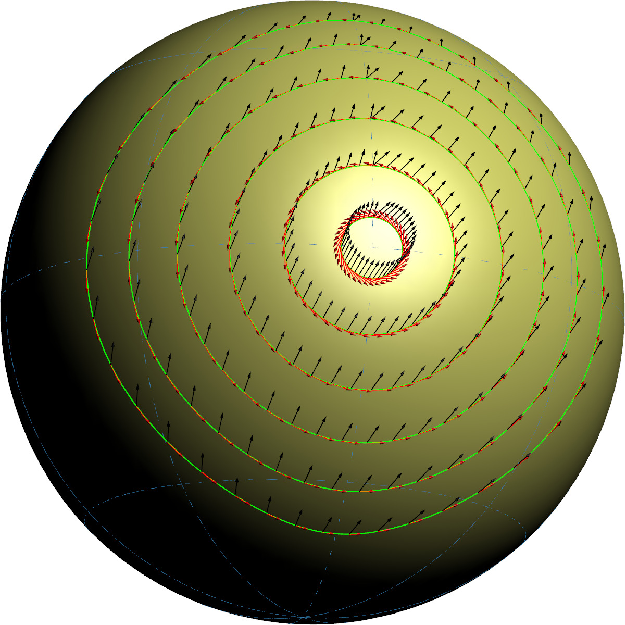
\includegraphics[scale=1]{parallel_transport1} 
	\end{center}
	\caption{Parallel transport for $u_{0}=0$ and $v_{0}=0$. Red vectors are tangents to circular curves and black vectors
	are the vectors being transported.}\label{fig1}
\end{figure}
\begin{figure}[h]
	\begin{center}
	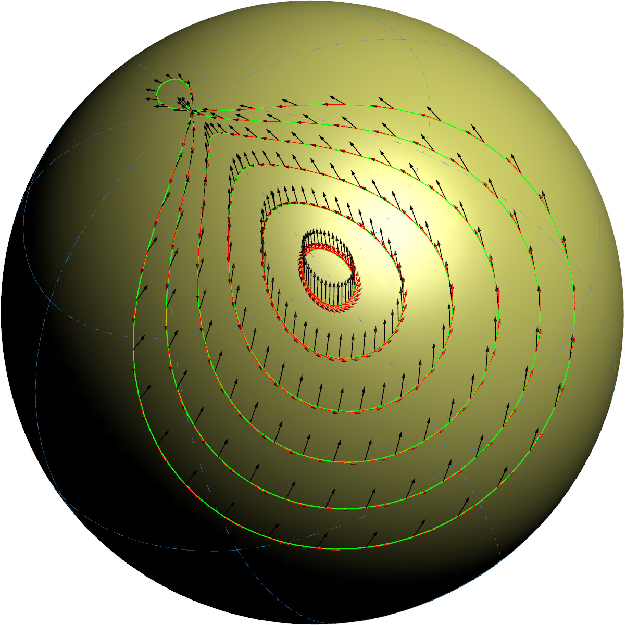
\includegraphics[scale=1]{parallel_transport2} 
	\end{center}
	\caption{Parallel transport for $u_{0}=\pi/4$ and $v_{0}=\pi/4$. Red vectors are tangents to circular curves and black vectors
	are the vectors being transported.}\label{fig2}
\end{figure}

If $\f{\gamma}{s} = \paren{\f{u}{s},\f{v}{s}}$ defines the transport curve then
\be
	\deriv{\gamma}{s}{} = \deriv{u}{s}{}\eb_{u}+\deriv{v}{s}{}\eb_{v}
\ee
and the transport equations are
\begin{align}
	\paren{\deriv{\gamma}{s}{}\cdot\nabla} f =& \paren{\deriv{u}{s}{}\pdiff{f^{u}}{u}+\deriv{v}{s}{}\pdiff{f^{u}}{v}
	                                            -\f{\sin}{u}\f{\cos}{u}\deriv{v}{s}{}f^{v}}\eb_{u}+\nonumber \\
	                                          & \paren{\deriv{u}{s}{}\pdiff{f^{v}}{u}+\deriv{v}{s}{}\pdiff{f^{v}}{v}
	                                            +\bfrac{\f{\cos}{u}}{\f{\sin}{u}}
	                                             \paren{\deriv{u}{s}{}f^{v}+\deriv{v}{s}{}f^{u}}}\eb_{u}  \nonumber \\
	                                         =& \paren{\deriv{f^{u}}{s}{}
	                                            -\f{\sin}{u}\f{\cos}{u}\deriv{v}{s}{}f^{v}}\eb_{u}+\nonumber \\
	                                          & \paren{\deriv{f^{v}}{s}{}
	                                            +\bfrac{\f{\cos}{u}}{\f{\sin}{u}}
	                                             \paren{\deriv{u}{s}{}f^{v}+\deriv{v}{s}{}f^{u}}}\eb_{u}  = 0  \\
	 \deriv{f^{u}}{s}{} =& \;\f{\sin}{u}\f{\cos}{u}\deriv{v}{s}{}f^{v} \\
	 \deriv{f^{v}}{s}{} =& \;-\bfrac{\f{\cos}{u}}{\f{\sin}{u}}
	                                             \paren{\deriv{u}{s}{}f^{v}+\deriv{v}{s}{}f^{u}}
\end{align}
If the tensor component representation is contra-variant (superscripts instead of subscripts) we must use the covariant component representation of
the vector arguements of the tensor, $a = a_{i}\eb^{i}$.  Then the definition of parallel transport gives
\begin{align}
	\paren{a\cdot\nabla_{x}}b =& a^{i}\partial_{x^{i}}\paren{b_{j}\eb^{j}} \nonumber \\
	                          =& a^{i}\paren{\paren{\partial_{x^{i}}b_{j}}\eb^{j} + b_{j}\partial_{x^{i}}\eb^{j}},
\end{align}
and we need
\be
	\paren{\partial_{x^{i}}b_{j}}\eb^{j} + b_{j}\partial_{x^{i}}\eb^{j} = 0. \label{eq111a}
\ee
To satisfy equation~(\ref{eq111a}) consider the following
\begin{align}
	\partial_{x^{i}}\paren{\eb^{j}\cdot\eb_{k}} =& 0 \nonumber \\
	\paren{\partial_{x^{i}}\eb^{j}}\cdot\eb_{k} + \eb^{j}\cdot\paren{\partial_{x^{i}}\eb_{k}} =& 0  \nonumber \\
	\paren{\partial_{x^{i}}\eb^{j}}\cdot\eb_{k} + \eb^{j}\cdot\eb_{l}\Gamma_{ik}^{l} =& 0 \nonumber \\
	\paren{\partial_{x^{i}}\eb^{j}}\cdot\eb_{k} + \delta_{l}^{j}\Gamma_{ik}^{l} =& 0 \nonumber \\
	\paren{\partial_{x^{i}}\eb^{j}}\cdot\eb_{k} + \Gamma_{ik}^{j} =& 0 \nonumber \\
	\paren{\partial_{x^{i}}\eb^{j}}\cdot\eb_{k} =& -\Gamma_{ik}^{j}
\end{align}
Now dot eq~(\ref{eq111a}) into $\eb_{k}$ giving\footnote{These equations also show that
\be
	\partial_{x^{i}}\eb^{j} = -\Gamma_{ik}^{j}\eb^{k}.
\ee}
\begin{align}
	\paren{\partial_{x^{i}}b_{j}}\eb^{j}\cdot\eb_{k} + b_{j}\paren{\partial_{x^{i}}\eb^{j}}\cdot\eb_{k} =& 0  \nonumber \\
	\paren{\partial_{x^{i}}b_{j}}\delta_{j}^{k} - b_{j}\Gamma_{ik}^{j} =& 0 \nonumber \\
	\paren{\partial_{x^{i}}b_{k}} = b_{j}\Gamma_{ik}^{j}.
\end{align}

\section{Covariant Derivative of Tensors}
The covariant derivative of a tensor field $\f{T}{a_{1},\dots,a_{r};x}$ ($x$ is the coordinate tuple of which $T$ can be a non-linear function) in the direction $a_{r+1}$ is (remember $a_{j} = a^{k_{j}}\eb_{k_{j}}$ and the $\eb_{k_{j}}$ can be functions of $x$)
the directional derivative of $\f{T}{a_{1},\dots,a_{r};x}$ where all the $a_{i}$ vector arguments of $T$ are parallel transported. 

Thus if we have a mixed representation of a tensor 
\be
\f{T}{a_{1},\dots,a_{r};x} = 
	\f{T\indices{_{i_{1}\dots i_{s}}^{i_{s+1}\dots i_{r}}}}{x}a^{i_{1}}\dots a^{i_{s}}a_{i_{s+1}}\dots a_{i_{r}},
\ee
the covariant derivative of the tensor is
\begin{align}
	\paren{a_{r+1}\cdot D} \f{T}{a_{1},\dots,a_{r};x} =& 
		\pdiff{T\indices{_{i_{1}\dots i_{s}}^{i_{s+1}\dots i_{r}}}}{x^{r+1}}a^{i_{1}}\dots a^{i_{s}}a_{i_{s+1}}\dots a_{i_{r}}
		a^{i_{r+1}} \nonumber \\
		&\hspace{-0.5in}+ \sum_{p=1}^{s}\pdiff{a^{i_{p}}}{x^{i_{r+1}}}T\indices{_{i_{1}\dots i_{s}}^{i_{s+1}\dots i_{r}}}a^{i_{1}}\dots
		\breve{a}^{i_{p}}\dots a^{i_{s}}a_{i_{s+1}}\dots a_{i_{r}}a^{i_{r+1}} \nonumber \\
		&\hspace{-0.5in}+ \sum_{q=s+1}^{r}\pdiff{a_{i_{p}}}{x^{i_{r+1}}}T\indices{_{i_{1}\dots i_{s}}^{i_{s+1}\dots i_{r}}}a^{i_{1}}\dots
		a^{i_{s}}a_{i_{s+1}}\dots\breve{a}_{i_{q}}\dots a_{i_{r}}a^{i_{r+1}} \nonumber \\
		=& \pdiff{T\indices{_{i_{1}\dots i_{s}}^{i_{s+1}\dots i_{r}}}}{x^{r+1}}a^{i_{1}}\dots a^{i_{s}}a_{i_{s+1}}\dots a^{r}_{i_{r}}
		a^{i_{r+1}} \nonumber \\
		&\hspace{-0.5in}- \sum_{p=1}^{s}\Gamma_{i_{r+1}l_{p}}^{i_{p}}T\indices{_{i_{1}\dots i_{p}\dots i_{s}}^{i_{s+1}
		\dots i_{r}}}a^{i_{1}}\dots
		a^{l_{p}}\dots a^{i_{s}}a_{i_{s+1}}\dots a_{i_{r}}a^{i_{r+1}} \nonumber \\
		&\hspace{-0.5in}+ \sum_{q=s+1}^{r}\Gamma_{i_{r+1}i_{q}}^{l_{q}}T\indices{_{i_{1}\dots i_{s}}^{i_{s+1}\dots i_{q}
		\dots i_{r}}}a^{i_{1}}\dots
		a^{i_{s}}a_{i_{s+1}}\dots a_{l_{q}}\dots a_{i_{r}}a^{i_{r+1}}	.	\label{eq126a}
\end{align}
From eq~(\ref{eq126a}) we obtain the components of the covariant derivative to be
\begin{align}
	\pdiff{T\indices{_{i_{1}\dots i_{s}}^{i_{s+1}\dots i_{r}}}}{x^{r+1}}
	- \sum_{p=1}^{s}\Gamma_{i_{r+1}l_{p}}^{i_{p}}T\indices{_{i_{1}\dots i_{p}\dots i_{s}}^{i_{s+1}\dots i_{r}}}
	+ \sum_{q=s+1}^{r}\Gamma_{i_{r+1}i_{q}}^{l_{q}}T\indices{_{i_{1}\dots i_{s}}^{i_{s+1}\dots i_{q}\dots i_{r}}}.
\end{align}
To extend the covariant derivative to tensors with multivector values in the tangent space (geometric algebra of the
tangent space) we start with the coordinate free definition of the covariant derivative of a conventional tensor using
the following notation.  Let $\f{T}{a_{1},\dots,a_{r};x}$ be a conventional tensor then the directional covariant 
derivative is
\be
	\paren{b\cdot D}T = a^{i_{1}}\dots a^{i_{r}}\paren{b\cdot\nabla}\f{T}{e_{i_{1}},\dots,e_{i_{r}};x}
						   -\sum_{j=1}^{r}\f{T}{a_{1},\dots,\paren{b\cdot\nabla}a_{j},\dots,a_{r};x}.	\label{eq137a}
\ee
The first term on the r.h.s. of eq~(\ref{eq137a}) is the directional derivative of $T$ if we assume that the component 
coefficients of each of the $a_{j}$ does not change if the coordinate tuple changes. The remaining terms in 
eq~(\ref{eq137a}) insure that for the totality of eq~(\ref{eq137a}) the directional derivative $\paren{b\cdot\nabla}T$
is the same as that when all the  $a_{j}$ vectors are parallel transported.  If in eq~(\ref{eq137a}) we let 
$b\cdot\nabla$ be the directional derivative for a multivector field we have generalized the definintion of covariant
derivative to include the cases where $\f{T}{a_{1},\dots,a_{r};x}$ is a multivector and not only a scalar.  Basically in 
eq~(\ref{eq137a}) the terms $\f{T}{e_{i_{1}},\dots,e_{i_{r}};x}$ are multivector fields and 
$\paren{b\cdot\nabla}\f{T}{e_{i_{1}},\dots,e_{i_{r}};x}$ is the direction derivative of each of the multivector fields that
make up the component representation of the multivector tensor.  The remaining terms in eq~(\ref{eq137a}) take into account
that for parallel transport of the $a_{i}$'s the coefficients $a^{i_{j}}$ are implicit functions of the coordinates
$x^{k}$. If we define the symbol $\nabla_{x}$ to only refer to taking the geometric derivative with respect to an explicit
dependence on the $x$ coordinate tuple we can recast eq~(\ref{eq137a}) into
\be
	\paren{b\cdot D}T = \paren{b\cdot\nabla_{x}}\f{T}{a_{1},\dots,a_{r};x}
						   -\sum_{j=1}^{r}\f{T}{a_{1},\dots,\paren{b\cdot\nabla}a_{j},\dots,a_{r};x}.	\label{eq137a}
\ee

\section{Coefficient Transformation Under Change of Variable}
In the previous sections on tensors a transformation of coordinate tuples 
$\f{\bar{x}}{x} = \paren{\f{\bar{x}^{i}}{x},\dots,\f{\bar{x}^{n}}{x}}$,
where $x=\paren{x^{1},\dots,x^{n}}$, is not mentioned since the definition of a tensor as a multilinear function is 
invariant to the representation of the vectors (coordinate system).  From our tensor definitions the effect of a coordinate
transformation on the tensor components is simply calculated.

If $\f{R}{x} = \f{R}{\bar{x}}$ is the defining vector function for a vector manifold ($R$ is in the embedding space of the
manifold) then\footnote{For an abstract manifold the equation $\bar{\eb}_{i} = \pdiff{x^{j}}{\bar{x}^{i}}\eb_{j}$ can be
used as an defining relationship.}
\begin{align}
	\eb_{i} =& \pdiff{R}{x^{i}} = \pdiff{\bar{x}^{j}}{x^{i}}\bar{\eb}_{j} \\
	\bar{\eb}_{i} =& \pdiff{R}{\bar{x}^{i}} =  \pdiff{x^{j}}{\bar{x}^{i}}\eb_{j}.
\end{align}
Thus we have
\begin{align}
	\f{T}{\eb_{i_{1}},\dots,\eb_{i_{1}}} =& T_{i_{1}\dots i_{r}} \\
	\f{T}{\bar{\eb}_{j_{1}},\dots,\bar{\eb}_{j_{1}}} =& \bar{T}_{j_{1}\dots j_{r}} \\
	\f{T}{\eb_{i_{1}},\dots,\eb_{i_{1}}} =& \f{T}{\pdiff{\bar{x}^{j_{1}}}{x^{i_{1}}}\bar{\eb}_{j_{1}},
	                                        \dots,\pdiff{\bar{x}^{j_{r}}}{x^{i_{r}}}\bar{\eb}_{j_{1}}} \\
	                                     =& \pdiff{\bar{x}^{j_{1}}}{x^{i_{1}}}\dots \pdiff{\bar{x}^{j_{r}}}{x^{i_{r}}}
	                                     \f{T}{\bar{\eb}_{j_{1}},\dots,\bar{\eb}_{j_{1}}} \\
	T_{i_{1}\dots i_{r}} =&  \pdiff{\bar{x}^{j_{1}}}{x^{i_{1}}}\dots\pdiff{\bar{x}^{j_{r}}}{x^{i_{r}}}
	                                     \bar{T}_{j_{1}\dots j{r}}. \label{eq7_51a} 
\end{align}
Equation~(\ref{eq7_51a}) is the standard formula for the transformation of tensor components.

\chapter[Lagrangian and Hamiltonian Methods]{Lagrangian and Hamiltonian Methods\footnote{This chapter follows ``A Multivector 
Derivative Approach to Lagrangian Field Theory,'' by A. Lasenby, C. Doran, and S. Gull, Feb. 9, 1993 available at http://www.mrao.cam.ac.uk/~cjld1/pages/publications.htm}}

\section{Lagrangian Theory for Discrete Systems}
\subsection{The Euler-Lagrange Equations}
Let a system be described by multivector variables $X_{i}$, $i=1,\dots,m$.  The Lagrangian $L$ is a scalar valued function of 
the $X_{i}$, $\dot{X}_{i}$ (here the dot refers to the time derivative), and possibly the time, $t$.  The action for the system, $S$,
over a time interval is given by the integral
\be
	S \equiv \int_{t_{1}}^{t_{2}}dt\f{L}{X_{i},\dot{X}_{i},t}.
\ee
The statement of the principal of least action is that the variation of the action $\delta S=0$.  The rigorous definition of $\delta S=0$ is
let 
\be
	\f{X'_{i}}{t} = \f{X_{i}}{t}+\epsilon\f{Y_{i}}{t}
\ee
where $\f{Y_{i}}{t}$ is an arbitrary differentiable multivector function of time except that $\f{Y_{i}}{t_{1}} = \f{Y_{i}}{t_{2}}=0$. Then
\be
	\delta S \equiv \eval{\deriv{S}{\epsilon}}{\epsilon=0} = 0.
\ee
Then
\begin{align}
    \f{L}{X'_{i},\dot{X}'_{i},t} &= \f{L}{X_{i}+\epsilon Y_{i},\dot{X}_{i}+\epsilon\dot{Y}_{i},t} \label{eq7_4a} \\
                                 &= \f{L}{X_{i},\dot{X}_{i},t}+\epsilon\sum_{i=1}^{m}\paren{Y_{i}*\pD{X_{i}}{L}+\dot{Y}_{i}*\pD{\dot{X}_{i}}{L}} \label{eq7_4b}\\
                               S &= \int_{t_{1}}^{t_{2}} dt\paren{\f{L}{X_{i},\dot{X}_{i},t}+\epsilon\sum_{i=1}^{m}\paren{Y_{i}*\pD{X_{i}}{L}
                                    +\dot{Y}_{i}*\pD{\dot{X}_{i}}{L}} } \\
	\eval{\deriv{S}{\epsilon}}{\epsilon=0} &= \int_{t_{1}}^{t_{2}}dt\sum_{i=1}^{m}\paren{Y_{i}*\partial_{X_{i}}L+\dot{Y}_{i}*\partial_{\dot{X}_{i}}L} \label{eq7_4} \\
	                                       &= \int_{t_{1}}^{t_{2}}dt\sum_{i=1}^{m}Y_{i}*\paren{\partial_{X_{i}}L-\deriv{}{t}\paren{\partial_{\dot{X}_{i}}L}} \label{eq7_5}                               
\end{align}
where we use the definition of the multivector derivative to go from equation~\ref{eq7_4a} to equation~\ref{eq7_4b} and then use integration by parts with respect
to time to go from equation~\ref{eq7_4} to equation~\ref{eq7_5}.  Since in equation~\ref{eq7_5} the $Y_{i}$'s are arbitrary $\delta S=0$ implies that the 
Lagrangian equations of motion are
\be
	\partial_{X_{i}}L-\deriv{}{t}\paren{\partial_{\dot{X}_{i}}L} = 0,\hspace{12pt}\forall i=1,\dots,m. \label{eq7_6}
\ee
The multivector derivative insures that there are as many equations as there are grades present in the $X_{i}$, which implies there are the same number of equations
as there are degrees of freedom in the system.

\subsection{Symmetries and Conservation Laws}\label{SandC}
Consider a scalar parametrised transformation of the dynamical variables
\be
	X'_{i} = \f{X'_{i}}{X_{i},\alpha},
\ee
where $\f{X'_{i}}{X_{i},0} = X_{i}$. Now define
\be
	\var{X_{i}} \equiv \eval{\deriv{X'_{i}}{\alpha}}{\alpha=0}.
\ee
and a transformed Lagrangian 
\be
	\f{L'}{X_{i},\dot{X}_{i},t} \equiv \f{L}{X'_{i},\dot{X}'_{i},t}.
\ee
Then
\begin{align}
	\eval{\deriv{L'}{\alpha}}{\alpha=0} &= \sum_{i=1}^{m}\paren{\var{X_{i}}*\partial_{X'_{i}}L'+\var{\dot{X}_{i}}*\partial_{\dot{X}'_{i}}L'} \nonumber \\
	                                    &= \sum_{i=1}^{m}\paren{\var{X_{i}}*\partial_{X'_{i}}L'
	                                       +\deriv{}{t}\paren{\var{X_{i}}*\partial_{\dot{X}'_{i}}L'}
	                                       -\var{X_{i}}*\deriv{}{t}\paren{\partial_{\dot{X}'_{i}}L'}} \nonumber \\
	                                    &= \sum_{i=1}^{m}\paren{\var{X_{i}}*\paren{\partial_{X'_{i}}L'
	                                       -\deriv{}{t}\paren{\partial_{\dot{X}'_{i}}L'}}
	                                       +\deriv{}{t}\paren{\var{X_{i}*\partial_{\dot{X}'_{i}}L'}}}. \label{eq7_13}
\end{align}
If the $X'_{i}$'s satisfy equation~\ref{eq7_6} equation~\ref{eq7_13} can be rewritten as
\be
	\eval{\deriv{L'}{\alpha}}{\alpha=0} = \deriv{}{t}\sum_{i=1}^{m}\paren{\var{X_{i}}*\partial_{\dot{X}_{i}}L}.\label{eq7_14}
\ee
Noether's theorem is -
\be\label{eqPPNT}
    \eval{\deriv{L'}{\alpha}}{\alpha=0}\hspace{-12pt} = 0 \implies \sum_{i=1}^{m}\paren{\var{X_{i}}*\partial_{\dot{X}_{i}}L} = \mbox{conserved quantity}
\ee

From D\& L -

``If the transformation is a symmetry of the Lagrangian, then $L'$ is independent of $\alpha$.  In this case we immediately establish that a conjugate quantity
is conserved.  That is, symmetries of the Lagrangian produce conjugate conserved quantities.  This is Noether's theorem, and it is valuable for extracting
conserved quantities from dynamical systems.  The fact that the derivation of equation~\ref{eq7_14} assumed the equations of motion were satisfied means that
the quantity is conserved `on-shell'.  Some symmetries can also be extended `off-shell', which becomes an important issue in quantum and super symmetric systems.''

A more general treatment of symmetries and conservation is possible if we do not limit ourselves to a scalar parametrization.  Instead let
$X'_{i} = \f{X'_{i}}{X_{i},M}$ where $M$ is a multivector parameter. Then let
\be
	L' = \f{L}{X'_{i},\dot{X}'_{i},t}
\ee
and calculate the multivector derivative of $L'$ with respect to $M$ using the chain rule (summation convention for repeated indices) first noting that
\be
	\pdiff{}{t}\paren{\paren{\paren{A*\partial_{M}}X'_{i}}*\partial_{\dot{X}'_{i}}L'} = \paren{\paren{A*\partial_{M}}\dot{X}'_{i}}*\partial_{\dot{X}'_{i}}L'
		+\paren{\paren{A*\partial_{M}}X'_{i}}*\pdiff{}{t}\paren{\partial_{\dot{X}'_{i}}L'}
\ee
and then calculating
\begin{align}
	\paren{A*\partial_{M}}L' &= \paren{\paren{A*\partial_{M}}X'_{i}}*\partial_{X'_{i}}L'
	                            +\paren{\paren{A*\partial_{M}}\dot{X}'_{i}}*\partial_{\dot{X}'_{i}}L' \nonumber \\
	                       &= \paren{\paren{A*\partial_{M}}X'_{i}}*\paren{\partial_{X'_{i}}L'-\pdiff{}{t}\paren{\partial_{\dot{X}'_{i}}L'}}
	                          +\pdiff{}{t}\paren{\paren{\paren{A*\partial_{M}}X'_{i}}*\partial_{\dot{X}'_{i}}L'}.
\end{align}
If we assume that the $X'_{i}$'s satisfy the equations of motion we have
\be
	\paren{A*\partial_{M}}L' = \pdiff{}{t}\paren{\paren{\paren{A*\partial_{M}}X'_{i}}*\partial_{\dot{X}'_{i}}L'}\label{eq7_22}
\ee
and differentiating equation~\ref{eq7_22} with respect to $A$ (use equation~\ref{eq6_40a}) gives
\begin{align}
	\partial_{M}L' &= \pdiff{}{t}\paren{\partial_{A}\paren{\paren{A*\partial_{M}}X'_{i}}*\partial_{\dot{X}'_{i}}L'} \nonumber \\
	               &= \pdiff{}{t}\paren{\paren{\partial_{M}X'_{i}}*\partial_{\dot{X}'_{i}}L'}. \label{eq7_25a} 
\end{align}
Equation~\ref{eq7_25a} is a generalization of Noether's theorem since if $\partial_{M}L'= 0$ then the parametrization $M$ is a symmetry of the Lagrangian
and $\paren{\partial_{M}X'_{i}}*\partial_{\dot{X}'_{i}}L'$ is a conserved quantity.

\subsection{Examples of Lagrangian Symmetries}

\subsubsection{Time Translation}

Consider the symmetry of time translation
\be
	\f{X'_{i}}{t,\alpha} = \f{X_{i}}{t+\alpha}
\ee 
so that 
\be
	\var{X_{i}} = \eval{\deriv{X'_{i}}{\alpha}}{\alpha=0} = \dot{X}_{i},
\ee
and
\begin{align}
	\left .\deriv{L}{\alpha}\right |_{\alpha=0} &= \deriv{}{t}\sum_{i=1}^{m}\paren{\dot{X}_{i}*\partial_{\dot{X}_{i}}L} \\
	0 &= \deriv{}{t}\paren{\sum_{i=1}^{m}\paren{\dot{X}_{i}*\partial_{\dot{X}_{i}}L}-L}.
\end{align}
The conserved quantity is the Hamiltonian
\be
	H = \sum_{i=1}^{m}\paren{\dot{X}_{i}*\partial_{\dot{X}_{i}}L}-L.
\ee
In terms of the generalized momenta
\be
	P_{i} = \partial_{\dot{X}_{i}}L,
\ee
so that
\be
	H = \sum_{i=1}^{m}\paren{\dot{X}_{i}*P_{i}}-L.
\ee


\subsubsection{Central Forces}
Let the Lagrangian variables be $x_{i}$ the vector position of the $i^{th}$ particle in an ensemble of $N$ particles with a Lagrangian of the form
\be
    L = \sum_{i=1}^{N}\half m_{i}\dot{x}_{i}^{2} - \sum_{i=1}^{N}\sum_{j<i}^{N}\f{V_{ij}}{\abs{x_{i}-x_{j}}}
\ee
which represent a classical system with central forces between each pair of particles.

First consider a translational invariance so that
\be
    x'_{i} = x_{i}+\alpha c
\ee
where $\alpha$ is a scalar parameter and $c$ is a constant vector.  Then
\be
    \delta x'_{i} = c
\ee
and
\be
    L' = L
\ee
so that the conserved quantity is (equation~\ref{eqPPNT})
\begin{align}
    \sum_{i=1}^{N}\delta x_{i} * \partial_{\dot{x_{i}}} L &= c * \sum_{i=1}^{N} \partial_{\dot{x_{i}}} L \nonumber \\
    c\cdot p &= c \cdot \sum_{i=1}^{N} m_{i}\dot{x}_{i} \nonumber \\
    p &= \sum_{i=1}^{N} m_{i}\dot{x}_{i}
\end{align}
since $c$ is an arbitrary vector the vector $p$ is also conserved and is the linear momentum of the system.

Now consider a rotational invariance where
\be
    x'_{i} = e^{\alpha B/2}x_{i}e^{-\alpha B/2}
\ee
where $B$ is an arbitrary normalized ($B^{2}=-1$) bivector in 3-dimensions and $\alpha$ is the scalar 
angle of rotation.  Then again $L' = L$ since rotations leave $\dot{x}_{i}^{2}$ and $\abs{x_{i}-x_{j}}$
unchanged and
\begin{align}
    \deriv{x'_{i}}{\alpha} &= \half\paren{Be^{\alpha B/2}x_{i}e^{-\alpha B/2}-e^{\alpha B/2}x_{i}e^{-\alpha B/2}B} \nonumber \\
    \delta x'_{i} &= \half\paren{Bx_{i}-x_{i}B} \nonumber \\
                  &= B\cdot x_{i}.
\end{align}
Remember that since $B\cdot x_{i}$ is a vector and the scalar product ($*$) of two vectors is the dot product we have for a 
conserved quantity
\begin{align}
  \sum_{i=1}^{N}\paren{B\cdot x_{i}}\cdot\paren{\partial_{\dot{x}_{i}}L} 
           &= \sum_{i=1}^{N}m_{i}\paren{B\cdot x_{i}}\cdot\dot{x}_{i} \label{eq7_35_s1}\\
           &= B\cdot \sum_{i=1}^{N}m_{i}\paren{x_{i}\W\dot{x}_{i}} \label{eq7_35_s2} \\
           &= B\cdot J \\
        J  &= \sum_{i=1}^{N}m_{i}\paren{x_{i}\W\dot{x}_{i}}
\end{align}
where we go from equation~\ref{eq7_35_s1} to equation~\ref{eq7_35_s2} by using the identity in equation~\ref{eq465a}. Then since 
equation~\ref{eq7_35_s1} is conserved for any bivector $B$, the angular momentum bivector, $J$, of the system is conserved.
\section{Lagrangian Theory for Continuous Systems}
For ease of notation we define
\be
	A\lgrad \equiv \dot{A}\dot{\nabla}.\label{eq7_24}
\ee
This is done for the situation that we are left differentiating a group of symbols.  For example consider
\be
	\paren{ABC}\lgrad = \dot{\paren{ABC}}\dot{\nabla}.\label{eq7_25}
\ee
The r.h.s. of equation~\ref{eq7_25} could be ambiguous in that could the overdot only apply to the $B$ variable.  Thus we will use the convention
of equation~\ref{eq7_24} to denote differentiation of the group immediately to the left of the derivative.  Another convention we could use to 
denote the same operation is
\be
	\widehat{ABC}\widehat{\nabla} = \paren{ABC}\lgrad
\ee
since using the ``hat'' symbol is unambiguous with respect to what symbols we are applying the differentiation operator to since the ``hat'' can extend
over all the relevant symbols.  
\subsection{The Euler Lagrange Equations}
Let $\f{\psi_{i}}{x}$ be a set of multivector fields and assume the Lagrangian density, $\Lf$, is a scalar function $\f{\Lf}{\psi_{i},\nabla\psi_{i},x}$ so
that the action, $S$, of the continuous system is given by
\be
	S = \int_{V}\abs{dx^{n}}\f{\Lf}{\psi_{i},\nabla\psi_{i},x},\label{eq7_27}
\ee
where $V$ is a compact $n$-dimensional volume.  The equations of motion are given by minimizing $S$ using the standard method of the calculus of 
variations where we define
\be
	\f{\psi'_{i}}{x} = \f{\psi_{i}}{x}+\epsilon\f{\phi_{i}}{x},
\ee
and assume that $\f{\psi_{i}}{x}$ yields an extrema of $S$ and that $\f{\phi_{i}}{x}=0$ for all $x\in\partial V$.  Then to get an extrema we need to define
\be
	\f{S}{\epsilon} = \int_{V}\abs{dx^{n}}\f{\Lf}{\psi_{i}+\epsilon\phi_{i},\nabla\psi_{i}+\epsilon\nabla\phi_{i},x},
\ee
so that $\f{S}{0}$ is an extrema if $\pdiff{S}{\epsilon} = 0$. Let us evaluate $\pdiff{S}{\epsilon}$ (summation convention)
\be
	\eval{\pdiff{S}{\epsilon}}{\epsilon=0} = \int_{V}\abs{dx^{n}}\paren{\paren{\phi_{i}*\partial_{\psi_{i}}}\Lf+\paren{\nabla\phi_{i}*\partial_{\nabla\psi_{i}}}\Lf}.\label{eq7_30}
\ee
Start by reducing the second term in the parenthesis on the r.h.s. of equation~\ref{eq7_30} using RR5 (Appendix~\ref{RRrules})
\begin{align}
	\paren{\nabla\phi_{i}*\partial_{\nabla\psi_{i}}}\Lf &= \grd{\paren{\nabla\phi_{i}}\partial_{\nabla\psi_{i}}}{}\Lf \nonumber \\
	                                                    &= \grd{\paren{\nabla\phi_{i}}\partial_{\nabla\psi_{i}}\Lf}{} \nonumber \\
	                                                    &= \grd{\nabla\paren{\phi_{i}\partial_{\nabla\psi_{i}}\Lf}
	                                                       -\widehat{\nabla}\phi_{i}\paren{\widehat{\partial_{\nabla\psi_{i}}\Lf}}}{} \nonumber \\
	                                                    &= \nabla\cdot\grd{\phi_{i}\partial_{\nabla\psi_{i}}\Lf}{1}
	                                                       -\grd{\widehat{\nabla}\phi_{i}\paren{\widehat{\partial_{\nabla\psi_{i}}\Lf}}}{} \nonumber \\
	                                                    &= \nabla\cdot\grd{\phi_{i}\partial_{\nabla\psi_{i}}\Lf}{1}
	                                                       -\grd{\phi_{i}\paren{\partial_{\nabla\psi_{i}}\Lf}\lgrad}{}  \nonumber \\   
	                                                    &= \nabla\cdot\grd{\phi_{i}\partial_{\nabla\psi_{i}}\Lf}{1}
	                                                       -\phi_{i}*\paren{\paren{\partial_{\nabla\psi_{i}}\Lf}\lgrad}.
\end{align}
So that equation~\ref{eq7_30} becomes
\begin{align}
	\eval{\pdiff{S}{\epsilon}}{\epsilon=0} &= 
	                       \int_{V}\abs{dx^{n}}\phi_{i}*\paren{\partial_{\psi_{i}}\Lf-\paren{\partial_{\grad\psi_{i}}\Lf}\lgrad}
	                       +\int_{V}\abs{dx^{n}}\nabla\cdot\grd{\phi_{i}\partial_{\nabla\psi_{i}}\Lf}{1} \nonumber \\
	                    &= \int_{V}\abs{dx^{n}}\phi_{i}*\paren{\partial_{\psi_{i}}\Lf-\paren{\partial_{\grad\psi_{i}}\Lf}\lgrad}
	                       +\int_{\partial V}\abs{dS^{n-1}}n\cdot\grd{\phi_{i}\partial_{\nabla\psi_{i}}\Lf}{1} \nonumber \\
	                    &= \int_{V}\abs{dx^{n}}\phi_{i}*\paren{\partial_{\psi_{i}}\Lf-\paren{\partial_{\grad\psi_{i}}\Lf}\lgrad} \label{eq7_32}.
\end{align}
The $\int_{V}\abs{dx^{n}}\nabla\cdot\grd{\phi_{i}\partial_{\nabla\psi_{i}}\Lf}{1}$ term is found to be zero by using the generalized divergence theorem (equation~\ref{eq_divth}) and the
fact that the $\phi_{i}$'s are zero on $\partial V$.  If $\phi_{i}$ is a pure $r$-grade multivector we have by the properties of
the scalar product the following Lagrangian field equations
\be
	\grade{\partial_{\psi_{i}}\Lf-\paren{\partial_{\grad\psi_{i}}\Lf}\lgrad}{r} = 0\label{eq7_33a}
\ee
or
\be
	\grade{\partial_{\psi_{i}^{\R}}\Lf-\nabla\paren{\partial_{\paren{\grad\psi_{i}}^{\R}}\Lf}}{r} = 0.\label{eq7_34b}
\ee
For the more general case of a $\phi_{i}$ being a mixed grade multivector the Lagrangian field equations are
\be
	\partial_{\psi_{i}}\Lf-\paren{\partial_{\grad\psi_{i}}\Lf}\lgrad = 0\label{eq7_33}
\ee
or
\be
	\partial_{\psi_{i}^{\R}}\Lf-\nabla\paren{\partial_{\paren{\grad\psi_{i}}^{\R}}\Lf} = 0.\label{eq7_34}
\ee
Note that since equation~\ref{eq7_33} is true for $\psi_{i}$ being any kind of multivector field we have derived the field equations for vectors, tensors (antisymmetric), spinors, or any combination thereof.
\subsection{Symmetries and Conservation Laws}
We proceed as in section~\ref{SandC} and let $\psi'_{i} = \f{\psi'_{i}}{\psi_{i},M}$ where $M$ is a multivector parameter. Then
\be
	\f{\Lf'}{\psi_{i},\nabla\psi_{i}} \equiv \f{\Lf}{\psi'_{i},\nabla\psi'_{i}}
\ee
and using equation~\ref{eq_chainrule} and RR5
\begin{align}
	\paren{A*\partial_{M}}\Lf' &= \paren{\paren{A*\partial_{M}}\psi'_{i}}*\paren{\partial_{\psi'_{i}}\Lf'}
	                      +\paren{\paren{A*\partial_{M}}\nabla\psi'_{i}}*\paren{\partial_{\nabla\psi'_{i}}\Lf'} \nonumber \\
	                   &= \paren{\paren{A*\partial_{M}}\psi'_{i}}*\paren{\partial_{\psi'_{i}}\Lf'}
	                      +\grd{\paren{\paren{A*\partial_{M}}\nabla\psi'_{i}}\paren{\partial_{\nabla\psi'_{i}}\Lf'}}{} \nonumber \\
	                   &= \paren{\paren{A*\partial_{M}}\psi'_{i}}*\paren{\partial_{\psi'_{i}}\Lf'}
	                      +\grd{\nabla\paren{\paren{\paren{A*\partial_{M}}\psi'_{i}}\paren{\partial_{\nabla\psi'_{i}}\Lf'}}
	                      -\widehat{\nabla}\paren{\paren{\paren{A*\partial_{M}}\psi'_{i}}\paren{\widehat{\partial_{\nabla\psi'_{i}}\Lf'}}}}{} \nonumber \\
	                   &= \paren{\paren{A*\partial_{M}}\psi'_{i}}*\paren{\partial_{\psi'_{i}}\Lf'}
	                      +\nabla\cdot\grd{\paren{\paren{A*\partial_{M}}\psi'_{i}}\paren{\partial_{\nabla\psi'_{i}}\Lf'}}{1}
	                      -\grd{\paren{\paren{A*\partial_{M}}\psi'_{i}}\paren{\partial_{\nabla\psi'_{i}}\Lf'}\lgrad}{} \nonumber \\
	                   &= \paren{\paren{A*\partial_{M}}\psi'_{i}}*\paren{\partial_{\psi'_{i}}\Lf'}
	                      +\nabla\cdot\grd{\paren{\paren{A*\partial_{M}}\psi'_{i}}\paren{\partial_{\nabla\psi'_{i}}\Lf'}}{1}
	                      -\paren{\paren{A*\partial_{M}}\psi'_{i}}*\paren{\partial_{\nabla\psi'_{i}}\Lf'}\lgrad \nonumber \\
	                   &= \paren{\paren{A*\partial_{M}}\psi'_{i}}*\paren{\paren{\partial_{\psi'_{i}}\Lf'}-\paren{\partial_{\nabla\psi'_{i}}\Lf'}\lgrad}
	                      +\nabla\cdot\grd{\paren{\paren{A*\partial_{M}}\psi'_{i}}\paren{\partial_{\nabla\psi'_{i}}\Lf'}}{1}
\end{align}
and if the Euler-Lagrange equations are satisfied we have
\be
    \paren{A*\partial_{M}}\Lf' = \nabla\cdot\grd{\paren{\paren{A*\partial_{M}}\psi'_{i}}\paren{\partial_{\nabla\psi'_{i}}\Lf'}}{1}
\ee
and by equation~\ref{eq6_40a}
\be
	\partial_{M}\Lf' = \partial_{A}\paren{\nabla\cdot\grd{\paren{\paren{A*\partial_{M}}\psi'_{i}}\paren{\partial_{\nabla\psi'_{i}}\Lf'}}{1}}. \label{eq7_37}
\ee
If $\partial_{M}\Lf'=0$, equation~\ref{eq7_37} is the most general form of Noether's theorem for the scalar valued multivector Lagrangian density.

If in equation~\ref{eq7_37} $M$ is a scalar $\alpha$ and $B$ is a scalar $\beta$ we have
\begin{align}
	\partial_{\alpha}\Lf' &= \partial_{\beta}\paren{\nabla\cdot\grd{\paren{\paren{\beta\partial_{\alpha}}\psi'_{i}}\paren{\partial_{\nabla\psi'_{i}}\Lf'}}{1}} \nonumber \\
	                      &= \nabla\cdot\grd{\paren{\partial_{\alpha}\psi'_{i}}\paren{\partial_{\nabla\psi'_{i}}\Lf'}}{1}.\label{eq7_38}
\end{align}
Thus if $\alpha=0$ in equation~\ref{eq7_38} we have
\be
	\eval{\partial_{\alpha}\Lf'}{\alpha=0} = \nabla\cdot\eval{\grd{\paren{\partial_{\alpha}\psi'_{i}}\paren{\partial_{\nabla\psi'_{i}}\Lf'}}{1}}{\alpha=0}
\ee
which corresponds to an differential transformation ($\partial_{\alpha}\Lf'=0$ is a global transformation). If $\eval{\partial_{\alpha}\Lf'}{\alpha=0}=0$ 
the conserved current is
\be
	j = \eval{\grd{\paren{\partial_{\alpha}\psi'_{i}}\paren{\partial_{\nabla\psi'_{i}}\Lf'}}{1}}{\alpha=0}
\ee
with conservation law
\be
	\nabla\cdot j = 0.
\ee
If $\eval{\partial_{\alpha}\Lf'}{\alpha=0}\ne 0$ we have by the chain rule that $\paren{\f{g}{x}=\eval{\partial_{\alpha}x'}{\alpha=0}}$
\be
	\eval{\partial_{\alpha}\Lf'}{\alpha=0} = \eval{\partial_{\alpha}x'}{\alpha=0}\cdot\eval{\nabla\Lf'}{\alpha=0} = \f{g}{x}\cdot\nabla\Lf
\ee
and consider
\be
	\nabla\cdot\paren{g\Lf} = \paren{\nabla\cdot g}\Lf+g\cdot\nabla\Lf.
\ee
If $\nabla\cdot g=0$ we can write $\eval{\partial_{\alpha}\Lf'}{\alpha=0}$ as a divergence so that
\be
	\nabla\cdot\paren{\grd{\paren{\eval{\partial_{\alpha}\psi'_{i}}{\alpha=0}}\paren{\partial_{\nabla\psi_{i}}\Lf}}{1}-\paren{\eval{\partial_{\alpha}x'}{\alpha=0}}\Lf} = 0
\ee
and
\be
	j = \grd{\paren{\eval{\partial_{\alpha}\psi'_{i}}{\alpha=0}}\paren{\partial_{\nabla\psi_{i}}\Lf}}{1}-\paren{\eval{\partial_{\alpha}x'}{\alpha=0}}\Lf
\ee
is a conserved current if $\nabla\cdot\eval{\partial_{\alpha}x'}{\alpha=0}=0$.

Note that since $\eval{\partial_{\alpha}x'}{\alpha=0}$ is the derivative of a vector with respect to a scalar it itself is a vector.  Thus the 
conserved $j$ is always a vector that could be a linear function of a vector, bivector, etc. depending upon the type of transformation (vector for affine
and bivector for rotation).  However, the conserved quantity of interest may be other than a
vector such as the stress-energy tensor or the angular momentum bivector.  In these cases the conserved vector current must be transformed to the
conserved quantity of interest via the general adjoint transformation $A*\f{\overline{j}}{B} = B*\f{\underline{j}}{A}$. 

\subsection{Space-Time Transformations and their Conjugate Tensors}
The canonical stress-energy tensor is the current associated with the symmetries of space-time translations. As a function of the parameter $\alpha$
we have
\begin{align}
	x' &= x+\alpha n \\
	\f{\psi'_{i}}{x} &= \f{\psi_{i}}{x+\alpha n}
\end{align}
Then
\begin{align}
	\eval{\partial_{\alpha}\Lf'}{\alpha=0} &= \eval{\partial_{\alpha}\f{\Lf}{x+\alpha n}}{\alpha=0} = n\cdot\nabla\Lf = \nabla\cdot\paren{n\Lf}\\
	\eval{\partial_{\alpha}\psi'_{i}}{\alpha=0} &= n\cdot\nabla\psi_{i}
\end{align}
and equation~\ref{eq7_38} becomes
\be
 	\nabla\cdot\paren{n\Lf} = \nabla\cdot\grd{\paren{n\cdot\nabla\psi_{i}}\paren{\partial_{\nabla\psi_{i}}\Lf}}{1}
\ee
so that
\be
	\nabla\cdot\f{\overline{T}}{n} \equiv \nabla\cdot\grd{\paren{n\cdot\nabla\psi_{i}}\paren{\partial_{\nabla\psi_{i}}\Lf}-n\Lf}{1} = 0. \label{eq7_47}
\ee
Thus the conserved current, $\f{\overline{T}}{n}$, is a linear vector function of a vector $n$, a tensor of rank 2.  In order put the stress-energy tensor
into the standard form we need the adjoint, $\f{\underline{T}}{n}$, of $\f{\overline{T}}{n}$ (we are using that the adjoint of the adjoint is the original
linear transformation). 
\begin{align}
	\f{\overline{T}}{n} &= \grd{\paren{n\cdot\nabla\psi_{i}}\paren{\partial_{\nabla\psi_{i}}\Lf}}{1}-n\Lf \\
	                    &= \paren{n\cdot\dot{\nabla}}\grd{\dot{\psi_{i}}\paren{\partial_{\nabla\psi_{i}}\Lf}}{1}-n\Lf.
\end{align}
Using equation~\ref{eq6_34a} we get
\begin{align}
	\f{\underline{T}}{n} &= \partial_{m}\grd{\paren{m\cdot\dot{\nabla}}\grd{\dot{\psi_{i}}\paren{\partial_{\nabla\psi_{i}}\Lf}}{1}n}{}-n\Lf \nonumber \\
	         &= \partial_{m}\paren{m\cdot\dot{\nabla}}\grd{\grd{\dot{\psi_{i}}\paren{\partial_{\nabla\psi_{i}}\Lf}}{1}n}{}-n\Lf \nonumber \\
	         &= \dot{\nabla}\grd{\grd{\dot{\psi_{i}}\paren{\partial_{\nabla\psi_{i}}\Lf}}{1}n}{}-n\Lf \nonumber \\
	         &= \dot{\nabla}\grd{\dot{\psi_{i}}\paren{\partial_{\nabla\psi_{i}}\Lf}n}{}-n\Lf. \label{eq7_70}
\end{align}
From equation~\ref{eq7_47} it follows that
\begin{align}
	0 = \nabla\cdot\f{\overline{T}}{n} &= n\cdot \f{\dot{T}}{\dot{\nabla}}, \\
	\f{\dot{T}}{\dot{\nabla}} &= 0,
\end{align}
or in rectangular coordinates
\be
	\f{\dot{T}}{\dot{\nabla}} = \f{\dot{T}}{e^{\mu}\dot{\pdiff{}{x^{\mu}}}} = \pdiff{}{x^{\mu}}\f{T}{e^{\mu}} 
	                           = \pdiff{T^{\mu\nu}}{x^{\mu}}e_{\nu}.
\ee
Thus in standard tensor notation
\be
	\pdiff{T^{\mu\nu}}{x^{\mu}} = 0,
\ee
so that $\f{T}{n}$ is a conserved tensor.

Now consider rotational transformations and for now assume the $\psi_{i}$ transform as vectors so that
\begin{align}
	x' &= e^{-\frac{\alpha B}{2}}xe^{\frac{\alpha B}{2}} \\
	\f{\psi'_{i}}{x} &= e^{\frac{\alpha B}{2}}\f{\psi_{i}}{x'}e^{-\frac{\alpha B}{2}}, 
\end{align}
Note that we are considering \emph{active} transformations.  The transformation of $x$ to $x'$ maps one distinct
point in space-time to another distinct point in space-time.  We are not considering \emph{passive} transformations
which are only a transformation of coordinates and the position vector does not move in space-time. Because the 
transformation is \emph{active} the sense of rotation of the vector field $\f{\psi}{x}$ is opposite that of the 
rotation of the space-time position vector\footnote{Consider an observer at location $x$ that is rotated to location $x'$. If he is 
rotated in a clockwise sense he observes the vector field to be rotating in a counter clockwise sense.}. Thus
\begin{align}
	\partial_{\alpha}x' &= \half e^{-\frac{\alpha B}{2}}\paren{xB-Bx}e^{\frac{\alpha B}{2}} \nonumber \\
	\eval{\partial_{\alpha}x'}{\alpha=0} &= x\cdot B \\	
	\partial_{\alpha}\psi'_{i} &= \half e^{\frac{\alpha B}{2}}\paren{B\f{\psi_{i}}{x'}-\f{\psi_{i}}{x'}B}e^{-\frac{\alpha B}{2}}
	                              +e^{\frac{\alpha B}{2}}\paren{\partial_{\alpha}\f{\psi_{i}}{x'}}e^{-\frac{\alpha B}{2}}  \nonumber \\
	                           &= e^{\frac{\alpha B}{2}}\paren{B\times\f{\psi_{i}}{x'}}e^{-\frac{\alpha B}{2}}
	                              +e^{\frac{\alpha B}{2}}\paren{\partial_{\alpha}x'\cdot\nabla\f{\psi_{i}}{x'}}e^{-\frac{\alpha B}{2}} \\
	\eval{\partial_{\alpha}\psi'_{i}}{\alpha=0} &= B\times \f{\psi_{i}}{x} +\eval{\partial_{\alpha}x'}{\alpha=0}\cdot\nabla\f{\psi_{i}}{x}  \nonumber \\
	                                            &= B\times \psi_{i} +\paren{x\cdot B}\cdot\nabla\psi_{i} =  \psi_{i}\cdot B +\paren{x\cdot B}\cdot\nabla\psi_{i}.          
\end{align}
Thus
\be
	\nabla\cdot\paren{\eval{\partial_{\alpha}x'}{\alpha=0}} = \nabla\cdot\paren{x\cdot B} = -\paren{B\cdot \dot{x}}\cdot\dot{\nabla} = -B\cdot\paren{\dot{x}\W\dot{\nabla}}
	                                           = B\cdot\paren{\nabla\W x} = 0
\ee
since $\nabla\W x = 0$\footnote{Consider
\begin{align*}\nabla\W x &= e^{\nu}\pdiff{}{x^{\nu}}\W x_{\eta}e^{\eta} \\
                         &= \pdiff{}{x^{\nu}}x_{\eta}e^{\nu}\W e^{\eta} \\
                         &= \pdiff{}{x^{\nu}}g_{\eta\mu}x^{\mu}e^{\nu}\W e^{\eta} \\
                         &= \pdiff{x^{\mu}}{x^{\nu}}g_{\eta\mu}e^{\nu}\W e^{\eta} \\
                         &= \delta^{\mu}_{\nu}g_{\eta\mu}e^{\nu}\W e^{\eta} \\
                         &= g_{\eta\nu}e^{\nu}\W e^{\eta} = 0
\end{align*}
since $g_{\eta\nu}$ is symmetric and $e^{\nu}\W e^{\eta} $ is antisymmetric.} the derivative of
the transformed Lagrangian at $\alpha = 0$ is a pure divergence,
\be
	\eval{\partial_{\alpha}\Lf'}{\alpha=0} = \nabla\cdot\paren{\paren{x\cdot B}\Lf}.
\ee
\begin{align}
	\eval{\nabla\cdot\grd{\paren{\partial_{\alpha}\psi'_{i}}\paren{\partial_{\nabla\psi'_{i}}\Lf}}{1}}{\alpha=0} &= 
		\nabla\cdot\grd{\paren{B\times\psi_{i}-\paren{B\cdot x}\cdot\nabla\psi_{i}}\paren{\partial_{\nabla\psi_{i}}\Lf}}{1}
\end{align}
\begin{align}
	\nabla\cdot\f{\overline{J}}{B} &\equiv \eval{\nabla\cdot\grd{\paren{\partial_{\alpha}\psi'_{i}}\paren{\partial_{\nabla\psi'_{i}}\Lf}}{1}}{\alpha=0}
	                                  -\eval{\partial_{\alpha}\Lf'}{\alpha=0} \nonumber \\
	                               &= \nabla\cdot\paren{\grd{\paren{B\times\psi_{i}-\paren{B\cdot x}\cdot\nabla\psi_{i}}\paren{\partial_{\nabla\psi_{i}}\Lf}}{1}-
	                                  \paren{x\cdot B}\Lf}
\end{align}
\be\label{eq7_67}
	\f{\overline{J}}{B} = \grd{\paren{B\times\psi_{i}-\paren{B\cdot x}\cdot\nabla\psi_{i}}\paren{\partial_{\nabla\psi_{i}}\Lf}}{1}-\paren{x\cdot B}\Lf.
\ee
By Noether's theorem $\dot{\nabla}\cdot\f{\dot{\overline{J}}}{B} = 0$ where $\f{\overline{J}}{B}$ is a conserved vector. So that
\begin{equation*}
	\dot{\nabla}\cdot\f{\dot{\overline{J}}}{B} = 0 \quad \Rightarrow \quad \f{\dot{\underline{J}}}{\dot{\nabla}}\cdot B = 0 \mbox{ for all } B 
	\quad\Rightarrow\quad \f{\dot{\underline{J}}}{\dot{\nabla}} = 0
\end{equation*}
The adjoint functon $\f{\underline{J}}{n}$ is, therefore a conserved bivector-valued function of position 
(we can use $\cdot$ instead of $*$ since all the grades match up correctly).

Now consider the coordinate (tensor) representation of $\f{\dot{\underline{J}}}{\dot{\nabla}} = 0$
\begin{align}
	n &= n_{\gamma}\bm{e}^{\gamma} \\
	\f{\underline{J}}{n} &= J^{\mu\nu\gamma}n^{\gamma}\bm{e}_{\mu}\W \bm{e}_{\nu} \\
	\f{\dot{\underline{J}}}{\dot{\nabla}} &= \pdiff{J^{\mu\nu\gamma}}{x^{\gamma}}\bm{e}_{\mu}\W \bm{e}_{\nu} = 0 \\
	\pdiff{J^{\mu\nu\gamma}}{x^{\gamma}} &= 0
\end{align}

To compute $\f{\underline{J}}{n}$ note that $A$ is a bivector using equation~\ref{eq6_34a}\footnote{$\f{\overline{F}}{B}=\partial_{A}\grd{\f{\underline{F}}{A}B}{}$} 
to calculate the adjoint of the adjoint
and $\paren{A*\partial_{B}}B = A$\footnote{$\paren{A*\partial_{B}}B = {\ds \lim_{h\rightarrow 0}}\bfrac{B+hA-B}{h}=A$} and 
RR7\footnote{$\paren{\grd{A}{2}\cdot a}\cdot b = \grd{A}{2}\cdot\paren{a\W b}$} we get
\begin{align}
	A*\f{\underline{J}}{n} &= \paren{A*\partial_{B}}\grd{\f{\overline{J}}{B}n}{} \nonumber \\
	                       &= \paren{A*\partial_{B}}\grd{\grd{\paren{B\times\psi_{i}-\paren{B\cdot x}\cdot\nabla\psi_{i}}\paren{\partial_{\nabla\psi_{i}}\Lf}}{1}n
	                          -\paren{x\cdot B}\Lf n}{} \nonumber \\
	                       &= \grd{\paren{A\times\psi_{i}-\paren{A\cdot x}\cdot\nabla\psi_{i}}\paren{\partial_{\nabla\psi_{i}}\Lf n}
	                          -\paren{x\cdot A}\Lf n}{} \nonumber \\
	                       &= \grd{\paren{A\times\psi_{i}-\paren{A\cdot\paren{x\W\nabla}}\psi_{i}}\paren{\partial_{\nabla\psi_{i}}\Lf n}
	                          -\paren{x\cdot A}\Lf n}{}. \label{eq7_68}  
\end{align}
Using RR5\footnote{$\grd{A_{1}\dots A_{k}}{}=\grd{A_{k}A_{1}\dots A_{k-1}}{}$} (Reduction Rule 5 in Appendix~\ref{RRrules}) the first term on the r.h.s.\;of equation~\ref{eq7_68} reduces to
\begin{align}
	\grd{\paren{A\times\psi_{i}}\paren{\partial_{\nabla\psi_{i}}\Lf n}}{} &= \half\grd{\paren{A\psi_{i}-\psi_{i}A}\paren{\partial_{\nabla\psi_{i}}\Lf n}}{} \nonumber \\
		&= \half\grd{A\brkt{\psi_{i}\paren{\partial_{\nabla\psi_{i}}\Lf n}-\paren{\partial_{\nabla\psi_{i}}\Lf n}\psi_{i}}}{}\nonumber \\
		&= \grd{A\paren{\psi_{i}\times\paren{\partial_{\nabla\psi_{i}}\Lf n}}}{} \nonumber \\
		&= A*\grd{\psi_{i}\times\paren{\partial_{\nabla\psi_{i}}\Lf n}}{2}, \label{eq7_69} 
\end{align}
using RR7 the second term reduces to 
\begin{align}
	\grd{\paren{A\cdot\paren{x\W\nabla}}\psi_{i}\paren{\partial_{\nabla\psi_{i}}\Lf n}}{} 
		&= \paren{A\cdot\paren{x\W\dot{\nabla}}}\grd{\dot{\psi}_{i}\partial_{\nabla\psi_{i}}\Lf n}{} \nonumber \\
		&= A*\paren{\paren{x\W\dot{\nabla}}\grd{\dot{\psi}_{i}\partial_{\nabla\psi_{i}}\Lf n}{}}, \label{eq7_70a}
\end{align}
using RR5 again the third term reduces to 
\begin{align}
	\grd{\paren{x\cdot A}\Lf n}{} &= \half\grd{\paren{xA-Ax}\Lf n}{} \nonumber \\
	                              &= \half\grd{A\paren{nx-xn}\Lf}{} \nonumber \\
	                              &= \grd{A\paren{n\W x}\Lf}{} \nonumber \\
	                              &= A*\paren{n\W x}\Lf. \label{eq7_71}
\end{align}
Combining equations~\ref{eq7_69}, \ref{eq7_70a}, and \ref{eq7_71} reduces equation~\ref{eq7_68} to
\be
	\f{\underline{J}}{n} = \grd{\psi_{i}\times\paren{\partial_{\nabla\psi_{i}}\Lf n}}{2}
	                      -\paren{x\W\dot{\nabla}}\grd{\dot{\psi}_{i}\partial_{\nabla\psi_{i}}\Lf n}{}
	                      -\paren{n\W x}\Lf \label{eq7_72}
\ee
where $\f{\underline{J}}{n}$ is the angular momentum bivector for the vector field.  Using equation~\ref{eq7_70a} we can reduce
equation~\ref{eq7_72} to
\be
	\f{\underline{J}}{n} = \f{T}{n}\W x + \grd{\psi_{i}\times\paren{\partial_{\nabla\psi_{i}}\Lf n}}{2}.
\ee

If $\psi_{i}$ is a spinor instead of a vector the transformation law is
\be
	\f{\psi'_{i}}{x} = e^{\frac{\alpha B}{2}}\f{\psi_{i}}{x'}
\ee
so that
\be
	\partial_{\alpha}\psi'_{i} = e^{\frac{\alpha B}{2}}\bfrac{B}{2}\f{\psi_{i}}{x'}+e^{\frac{\alpha B}{2}}\partial_{\alpha}x'\f{\psi_{i}}{x'}
\ee
and
\be
	\eval{\partial_{\alpha}\psi'_{i}}{\alpha=0} = \bfrac{B}{2}\psi_{i}+\paren{x\cdot B}\cdot\nabla\psi_{i}.
\ee
Equations~\ref{eq7_67} and \ref{eq7_72} become
\be
	\f{\overline{J}}{B} = \grd{\paren{\bfrac{B}{2}\psi_{i}-\paren{B\cdot x}\cdot\nabla\psi_{i}}\paren{\partial_{\nabla\psi_{i}}\Lf}}{1}-\paren{x\cdot B}\Lf
\ee
and
\be
	\f{\underline{J}}{n} = \grd{\bfrac{\psi_{i}}{2}\paren{\partial_{\nabla\psi_{i}}\Lf n}}{2}
	                      -\paren{x\W\dot{\nabla}}\grd{\dot{\psi}_{i}\partial_{\nabla\psi_{i}}\Lf n}{}
	                      -\paren{n\W x}\Lf
\ee
where $\f{\underline{J}}{n}$ is the angular momentum bivector for the spinor field.

Since spinors transforms the same as vectors under translations the expression (equation~\ref{eq7_70}) for the stress-energy tensor of a spinor field is the same as for a vector or scalar field, $\f{\underline{T}}{n} = \dot{\nabla}\grd{\dot{\psi_{i}}\paren{\partial_{\nabla\psi_{i}}\Lf}n}{}-n\Lf$, so that
\be
	\mbox{Spinor Field: }\f{\underline{J}}{n} = \f{\underline{T}}{n}\W x + \grd{\bfrac{\psi_{i}}{2}\paren{\partial_{\nabla\psi_{i}}\Lf n}}{2},
\ee
compared to
\be
	\mbox{Vector Field: }\f{\underline{J}}{n} = \f{T}{n}\W x + \grd{\psi_{i}\times\paren{\partial_{\nabla\psi_{i}}\Lf n}}{2}.
\ee

\subsection{Case 1 - The Electromagnetic Field}

Example of Lagrangian densities are the electromanetic field and the spinor field for an electron.  For the electromagnetic field we have
\be
	\mathcal{L} = \half F\cdot F - A\cdot J
\ee
where F = $\nabla\W A$ and using eq~\ref{eq6_15} and eq~\ref{eq6_17}
\begin{align}
		F\cdot F &= \grade{\paren{\nabla \W A}\paren{\nabla \W A}}{} \nonumber \\
		         &= \grade{\half\paren{\nabla A - \paren{\nabla A }^{\R}}\half\paren{\nabla A - \paren{\nabla A }^{\R}}}{} 
		            \nonumber \\
				 &= \bfrac{1}{4}\grade{\paren{\nabla A - \paren{\nabla A}^{\R}}^{2}}{} \nonumber \\
		         &= \bfrac{1}{4}\grade{\nabla A\nabla A-\nabla A\paren{\nabla A}^{\R}
		            -\paren{\nabla A}^{\R}\nabla A + \paren{\nabla A}^{\R}\paren{\nabla A}^{\R}}{} \nonumber \\
		         &= \bfrac{1}{4}\paren{\paren{\nabla A}*\paren{\nabla A} - \paren{\nabla A}*\paren{\nabla A}^{\R}
		           -\paren{\nabla A}^{\R}*\paren{\nabla A}+ \paren{\nabla A}^{\R}*\paren{\nabla A}^{\R}} \nonumber \\
		         &= \half\paren{\paren{\nabla A}*\paren{\nabla A} - \paren{\nabla A}*\paren{\nabla A}^{\R}}
\end{align}
Now calculate using eq~\ref{eq6_47a} and eq~\ref{eq6_51a}
\begin{align}
	\partial_{\paren{\nabla A}^{\R}} F^{2} &= \half\partial_{\paren{\nabla A}^{\R}}
	                                          \paren{\paren{\nabla A}*\paren{\nabla A} - \paren{\nabla A}*\paren{\nabla A}^{\R}}
	                                          \nonumber \\
	                                       &= \paren{\nabla A}^{\R} - \nabla A \nonumber \\
	                                       &= -2\nabla \W A
\end{align}
We also have by eq~\ref{eq6_44a} and that $A^{\R} = A$
\begin{align}
	\partial_{A^{\R}}\paren{A\cdot J} &= \partial_{A^{\R}}\paren{J * A} \nonumber \\
	                                  &= J
\end{align}
so that
\begin{align}
	\partial_{A^{\R}}\mathcal{L}-\nabla\paren{\partial_{\paren{\nabla A}^{\R}}\mathcal{L}} &= 
		J - \nabla\paren{\nabla \W A} = 0 \\
		\nabla F &= J
\end{align}




\subsection{Case 2 - The Dirac Field}
For the Dirac field
\begin{align}
		\mathcal{L} &= \grade{\nabla\psi I\gamma_{z}\psi^{\R}-eA\psi\gamma_{t}\psi^{\R}-m\psi\psi^{\R}}{} \nonumber \\
		            &= \paren{\nabla\psi}*\paren{I\gamma_{z}\psi^{\R}}-\grade{eA\psi\gamma_{t}\psi^{\R}}{} - m\psi*\psi^{\R} 
		               \label{eq8_110}\\
		            &= \paren{\nabla\psi I\gamma_{z}}*\psi^{\R}-\grade{eA\psi\gamma_{t}\psi^{\R}}{} - m\psi*\psi^{\R} \label{eq8_111}
\end{align}
The only term in eq~\ref{eq8_110} and eq~\ref{eq8_111} that we cannot immediately differentiate is 
$\partial_{\psi^{\R}}\grade{eA\psi\gamma_{t}\psi^{\R}}{}$. To perform this operation let $\psi^{\R} = X$ and use the definition of
the scalar directional derivative
\begin{align}
	\paren{B*\partial_{X}}\grade{eAX^{\R}\gamma_{t}X}{} &= 
		\lim_{h\rightarrow0}\bfrac{\grade{eA\paren{X^{\R}+hB^{\R}}\gamma_{t}\paren{X+hB}-eAX^{\R}\gamma_{t}X}{}}{h} \nonumber \\
		&= \grade{eAB^{\R}\gamma_{t}X+eAX^{\R}\gamma_{t}B}{} \nonumber \\
		&= B^{\R}*\paren{e\gamma_{t}XA}+B*\paren{eAX^{\R}\gamma_{t}} \nonumber \\
		&= B*\paren{eAX^{\R}\gamma_{t}}+B*\paren{eAX^{\R}\gamma_{t}} \nonumber \\
		&= B*\paren{2eAX^{\R}\gamma_{t}} \\
	 \partial_{X}\grade{eAX^{\R}\gamma_{t}X}{} &= 2eAX^{\R}\gamma_{t} \\
	 \partial_{\psi^{\R}}\grade{eA\psi\gamma_{t}\psi^{\R}}{} &= 2eA\psi\gamma_{t}
\end{align}
The other multivector derivatives are evaluated using the formulas in section~\ref{MV_derivatives}
\begin{align}
	\partial_{\paren{\nabla \psi}^{\R}} \paren{\paren{\nabla\psi}*\paren{I\gamma_{z}\psi^{\R}}} &=  \psi\gamma_{z}I^{\R} 
		= \psi\gamma_{z}I = -\psi I\gamma_{z} \\
	\partial_{\psi^{\R}}\paren{\paren{\nabla\psi I\gamma_{z}}*\psi^{\R}} &= \nabla\psi I\gamma_{z} \\
	\partial_{\psi^{\R}}\paren{m\psi*\psi^{\R}} &= 2m\psi.
\end{align}
The Lagrangian field equation are then
\begin{align}
	\partial_{\psi^{\R}}\mathcal{L}-\nabla\paren{\partial_{\paren{\nabla \psi}^{\R}}\mathcal{L}} &= \nabla\psi I\gamma_{z}
		-2eA\psi\gamma_{t}-2m\psi+\nabla\psi I\gamma_{z} = 0 \nonumber \\
		&= 2\paren{\nabla\psi I\gamma_{z}-eA\psi\gamma_{t}-m\psi} = 0 \nonumber \\
		0 &= \nabla\psi I\gamma_{z}-eA\psi\gamma_{t}-m\psi.
\end{align}

\subsection{Case 3 - The Coupled Electromagnetic and Dirac Fields}

For coupled electromagnetic and electron (Dirac) fields the coupled Lagrangian is 
\begin{align}
		\mathcal{L} &= \grade{\nabla\psi I\gamma_{z}\psi^{\R}-eA\psi\gamma_{t}\psi^{\R}-m\psi\psi^{\R}+\half F^{2}}{} \nonumber \\
		            &= \paren{\nabla\psi}*\paren{I\gamma_{z}\psi^{\R}}-\grade{eA\psi\gamma_{t}\psi^{\R}}{} - m\psi*\psi^{\R} 
		               +\half F^{2} \\
		            &= \paren{\nabla\psi I\gamma_{z}}*\psi^{\R}-eA*\paren{\psi\gamma_{t}\psi^{\R}} - m\psi*\psi^{\R} +\half F^{2},
\end{align}
where $A$ is the 4-vector potential dynamical field and $\psi$ is the spinor dynamical field. Between the previously calculated 
multivector derivatives for the electromagnetic and Dirac fields the only new derivative that needs to be calculated for the 
Lagrangian field equations is 
\begin{align}
	\partial_{A^{\R}}\paren{eA*\paren{\psi\gamma_{t}\psi^{\R}}} &= e\paren{\psi\gamma_{t}\psi^{\R}}^{\R} = e\psi\gamma_{t}\psi^{\R}.
\end{align}
The Lagrangian equations for the coupled fields are then
\begin{align}
	\partial_{\psi^{\R}}\mathcal{L} -\nabla\paren{\partial_{\paren{\nabla \psi}^{\R}}\mathcal{L}} &=
		2\paren{\nabla\psi I\gamma_{z}-eA\psi\gamma_{t}-m\psi} = 0 \\
	\partial_{A^{\R}}\mathcal{L} -\nabla\paren{\partial_{\paren{\nabla A}^{\R}}\mathcal{L}} &= 
		-e\psi\gamma_{t}\psi^{\R}+\nabla\paren{\nabla \W A} = 0
\end{align}
or
\begin{align}
	\nabla\psi I\gamma_{z}-eA\psi\gamma_{t} &= m\psi \\
	\nabla F = e\psi\gamma_{t}\psi^{\R}.
\end{align}
\chapter[Lie Groups as Spin Groups]{Lie Groups as Spin Groups\footnote{This chapter follows \cite{DHS&VA}}}

\section{Introduction}

A Lie group, $G$, is a group that is also a differentiable manifold. So that if $g \in G$ and $x \in \Re^{N}$ then
there is a differentiable mapping $\phi:\Re^{N}\rightarrow G$ so that for each $g \in G$ we can define a tangent 
space $\mathcal{T}_{g}$.

A example (the one we are most concerned with) of a Lie group is the group of $n\times n$ non-singular matrices.  The 
coordinates of the manifold are simply the elements of the matrix so that the dimension of the group manifold is $n^{2}$
and the matrix is obviously a continuous differentiable function of its coordinates.

A Lie algebra is a vector space $\mfrk{g}$ with a bilinear operator $\mat{\cdot,\cdot}:\mfrk{g}\times\mfrk{g}\rightarrow\mfrk{g}$
called the \emph{Lie bracket} which satifies ($x,y,z \in\mfrk{g}$ and $\alpha,\beta\in\Re$):
\begin{align}
	\mat{ax+by,z} &=a\mat{x,z}+b\mat{y,z}, \label{la1ax}\\
	\mat{x,x} &= 0, \label{la2ax}\\
	\mat{x,\mat{y,z}}+\mat{z,\mat{x,y}}+\mat{y,\mat{z,x}} &= 0\label{la3ax}.
\end{align}
Equations~(\ref{la1ax}) and (\ref{la2ax}) imply $\mat{x,y} = -\mat{y,x}$, while eq~(\ref{la3ax}) is the Jacobi identity.

The purpose of the following analysis is to show that the Lie algebra of the general linear group of dimension $n$
over the real numbers (the group of $n\times n$ invertible matrices), $GL\paren{n,\Re}$, can be represented by a rotation
group in an appropriate vector space, $\mathcal{M}$ (let $\paren{p,q}$ be the signature of the new vector space). Furthermore, 
since the rotation group, $SO\paren{p,q}$ can be represented by the spin group, $Spin\paren{p,q}$, in the same vector space. Then by use of
geometric algebra we can construct any rotor, $R\in Spin\paren{p,q}$, as $R = e^{\frac{B}{2}}$ where $B$ is a bi-vector in the geometric 
algebra of $\mathcal{M}$ and the bi-vectors form a Lie algebra under the commutator product.\footnote{Since we could be dealing with
vector spaces of arbitrary signature $\paren{p,q}$ we use the following nomenclature:
\begin{center}\begin{tabular}{cl}
	$\f{SO}{p,q}$  & Special orthogonal group in vector space with signature $\paren{p,q}$ \\
	$\f{SO}{n}$  & Special orthogonal group in vector space with signature $\paren{n,0}$ \\
	$\f{Spin}{p,q}$  & Spin group in vector space with signature $\paren{p,q}$ \\
	$\f{Spin}{n}$  & Spin group in vector space with signature $\paren{n,0}$ \\
	$\f{GL}{p,q,\Re}$  & General linear group in real vector space with signature $\paren{p,q}$ \\
	$\f{GL}{n,\Re}$  & General linear group in real vector space with signature $\paren{n,0}$
\end{tabular}\end{center}}

The main trick in doing this is to construct the appropriate vector space, $\mathcal{M}$, with subspaces isomorphic to $\Re^{n}$
so that a rotation in $\mathcal{M}$ is equivalent to a general linear transformation in a subspace of $\mathcal{M}$ isomorphic 
to $\Re^{n}$.  We might suspect that $\mathcal{M}$ cannot be a Euclidean space since a general linear transformation can cause
the input vector to grow as well as shrink.

\section{Simple Examples}

\subsection{$\f{SO}{2}$ - Special Orthogonal Group of Order 2}

The group is represented by all $2\times 2$ real matrices\footnote{We denote linear transformations with an underbar.} $\ubar{R}$ where\footnote{In this case $\ubar{I}$ is the identity matrix and not the
pseudo scalar.} $\ubar{R}\ubar{R}^{T} = \ubar{I}$ and $\det\paren{\ubar{R}} = 1$.  The group product is
matrix multiplication and it is a group since if $\ubar{R}_{1}\ubar{R}_{1}^{T} = \ubar{I}$ and $\ubar{R}_{2}\ubar{R}_{2}^{T} = \ubar{I}$ then
\begin{align}
	 \paren{\ubar{R}_{1}\ubar{R}_{2}}\paren{\ubar{R}_{1}\ubar{R}_{2}}^{T} &= \ubar{R}_{1}\ubar{R}_{2}\ubar{R}_{2}^{T}\ubar{R}_{1}^{T} = \ubar{R}_{1}\ubar{I}\ubar{R}_{1}^{T} = \ubar{R}_{1}\ubar{R}_{1}^{T} = \ubar{I} \\
	 \f{\det}{\ubar{R}_{1}\ubar{R}_{2}} &= \f{\det}{\ubar{R}_{1}}\f{\det}{\ubar{R}_{2}} = 1.
\end{align}
$SO\paren{2}$ is also a Lie group since all $\ubar{R}\in\f{SO}{2}$ can be represented as a continuous function of the coordinate $\theta$:
\begin{equation}
	\f{\ubar{R}}{\theta} = \mat{
	\begin{array}{cc}
		\f{\cos}{\theta} & -\f{\sin}{\theta} \\
		\f{\sin}{\theta} & \f{\cos}{\theta}
	\end{array}
	}.
\end{equation}
In this case the spin representation of $\f{SO}{2}$ is trivial, namely\footnote{For multivectors such as the rotor $R$ there is no 
underbar. We have $\f{\ubar{R}}{a} = \ubar{R}a = RaR^{\R}$ where $a$ is a vector.}
$\f{R}{\theta} = e^{\frac{I}{2}\theta} = \f{\cos}{\frac{\theta}{2}} + I\f{\sin}{\frac{\theta}{2}}$, 
$\f{R}{\theta}^{\R} = e^{-\frac{I}{2}\theta} = \f{\cos}{\frac{\theta}{2}} - I\f{\sin}{\frac{\theta}{2}}$ where $I$
is the pseudo-scalar for $\f{\mathcal{G}}{\Re^{2}}$. Then we have $\f{\ubar{R}}{\theta}a = \f{R}{\theta}a\f{R}{\theta}^{\R}$.

\subsection{$\f{GL}{2,\Re}$ - General Real Linear Group of Order 2}

The group is represented by all $2\times 2$ real matrices $\ubar{A}$ where $\f{\det}{\ubar{A}} \ne 0$.  Again the the group product is
matrix multiplication and it is a group because if $\ubar{A}$ and $\ubar{B}$ are $2\times 2$ real matrices then 
$\f{\det}{\ubar{A}\ubar{B}} = \f{\det}{\ubar{A}}\f{\det}{\ubar{B}}$ and if $\f{\det}{\ubar{A}}\ne 0$ and $\f{\det}{\ubar{B}}\ne 0$ then $\f{\det}{\ubar{A}\ubar{B}}\ne 0$.  Any member of 
the group is represented by the matrix $\paren{a = \paren{a^{1},a^{2},a^{3},a^{4}}\in \Re^{4}}$:
\begin{equation}
	\f{\ubar{A}}{a} = \mat{
	\begin{array}{cc}
		a^{1} & a^{2} \\
		a^{3} & a^{4}
	\end{array}
	}.
\end{equation}
Thus any element $\ubar{A}\in \f{GL}{2,\Re}$ is a continuous function of $a = \paren{a^{1},a^{2},a^{3},a^{4}}$.  Thus $\f{GL}{2,\Re}$ is a four
dimensional Lie group while $\f{SO}{2}$ is a one dimensional Lie group.

Another difference is that  $\f{SO}{2}$ is compact while $\f{GL}{2,\Re}$ is not.  $\f{SO}{2}$ is compact since for any
convergent sequence $\paren{\theta_{i}}$,
\begin{equation*}
	\lim_{i\rightarrow\infty}\f{\ubar{R}}{\theta_{i}}\in \f{SO}{2}.
\end{equation*} 
$\f{GL}{2,\Re}$ is not compact since there is at least one convergent sequence $\paren{a_{i}}$ 
such that
\begin{equation*}
	\lim_{i\rightarrow\infty}\f{\det}{\f{\ubar{A}}{a_{i}}} = 0.
\end{equation*} 
After we develop the required theory we will calculate the spin representation of $\f{GL}{2,\Re}$.

\section{The Grassmann Algebra}

Let $\mathcal{V}^{n}$ be an $n$-dimensional real vector space with basis $\set{\wb_{i}}: 1\le i \le n$ and $\W$ is the
outer (wedge) product for the geometric algebra define on $\mathcal{V}^{n}$. As before the geometric object
\be
	v_{1}\W v_{2}\W\dots\W v_{k}
\ee
is a $k$-blade in the Grassmann or the geometric algebra where the $v_{i}$'s are $k$ independent vectors in
$\mathcal{V}_{n}$ and a linear combination of $k$-blades is called a $k$-vector.  The space of all $k$-vectors is
just all the $k$-grade multivectors in the geometric algebra $\GA{\mathcal{V}_{n}}$. Denote the space of all
$k$-vectors in $\mathcal{V}^{n}$ by $\Lambda_{n}^{k} = \f{\Lambda^{k}}{\mathcal{V}^{n}}$ with
\be
	\f{\dim}{\Lambda_{n}^{k}} = \binom{n}{k} = \bfrac{n!}{k!\paren{n-k}!}.
\ee
Letting $\Lambda_{n}^{1} = \mathcal{V}^{n}$ and $\Lambda_{n}^{0} = \Re$ the entire Grassmann algebra is a 
$2^{n}$-dimensional space.\footnote{Consider the geometric algebra $\GA{\mathcal{V}^{n}}$ of $\mathcal{V}^{n}$
with a null basis $\set{\wb_{i}}:\wb_{i}^{2}=0,1\le i \le n$. Then 
\begin{align*}
	\paren{\wb_{i}+\wb_{j}}^2 &= \wb_{i}^{2}+\wb_{i}\wb_{j}+\wb_{j}\wb_{i}+\wb_{j}^{2} \\
	                        0 &= \wb_{i}\wb_{j}+\wb_{j}\wb_{i} \\
	                        \wb_{i}\wb_{j} &= -\wb_{j}\wb_{i} \\
	                        0 &= 2\wb_{i}\cdot\wb_{j}.
\end{align*}
If the basis set is null the metric tensor is null and $\wb_{i}\wb_{j} = \wb_{i}\W\wb_{j}$ even if $i=j$ and the geometric
algebra is a Grassmann algebra.}
\be
	\Lambda_{n} = \sum_{k=0}^{n} \Lambda_{n}^{k}.
\ee
The Grassmann algebra of a vector space $\mathcal{V}^{n}$ is denoted by $\f{\Lambda}{\mathcal{V}^{n}}$.


\section{The Dual Space to $\mathcal{V}_{n}$}

The dual space $\mathcal{V}^{n*}$ to $\mathcal{V}^{n}$ is defined as follows.  Let $\set{\wb_{i}}$ be a
basis for $\mathcal{V}^{n}$ and define the basis, $\set{\wb_{i}^{*}}$ for $\mathcal{V}^{n*}$ by
\be\label{eq8_4}
	\wb_{i}^{*}\cdot \wb_{j} = \half\delta_{ij}. 
\ee
Again the dual space $\mathcal{V}^{n*}$ has its own Grassmann algebra $\f{\Lambda^{*}}{\mathcal{V}^{n}}$
given by
\be
	\f{\Lambda^{*}}{\mathcal{V}^{n}} = \Lambda^{*}_{n} = \sum_{k=0}^{n}\Lambda_{n}^{k*}.
\ee
$\f{\Lambda^{*}}{\mathcal{V}^{n}}$ can be represented as a geometric algebra by imposing the null metric condition
$\paren{\wb_{i}^{*}}^{2}=0$ as in the case of $\f{\Lambda}{\mathcal{V}^{n}}$. 

\section{The Mother Algebra}

From the base vector space and it's 
dual space one can construct a $2n$ dimensional vector space from the direct sum of the two vector 
spaces as defined in Appendix~\ref{DSVS}
\be\label{eq8_6}
	\Re^{n,n} \equiv \mathcal{V}^{n}\oplus \mathcal{V}^{n*}
\ee
with basis $\set{\wb_{i},\wb_{j}^{*}}$.  An orthogonal basis for $\Re^{n,n}$ can be constructed as follows (using
equation~\ref{eq8_4}):
\begin{align}
	\eb_{i} &= \wb_{i}+\wb_{i}^{*} \label{eq8_7}\\
	\ebb_{i} &= \wb_{i}-\wb_{i}^{*} \label{eq8_7a}\\
	\eb_{i}\cdot\eb_{j} &= \paren{\wb_{i}+\wb_{i}^{*}}\cdot\paren{\wb_{j}+\wb_{j}^{*}} \nonumber \\
	                    &=  \wb_{i}\cdot\wb_{j}+\wb_{i}\cdot\wb_{j}^{*}+\wb_{i}^{*}\cdot\wb_{j}+
	                        \wb_{i}^{*}\cdot\wb_{j}^{*} \nonumber \\
	                    &= \delta_{ij} \label{eiej}\\
	\ebb_{i}\cdot\ebb_{j} &= \paren{\wb_{i}-\wb_{i}^{*}}\cdot\paren{\wb_{j}\wb_{j}^{*}} \nonumber \\
	                    &=  \wb_{i}\cdot\wb_{j}\wb_{i}\cdot\wb_{j}^{*}-\wb_{i}^{*}\cdot\wb_{j}+
	                        \wb_{i}^{*}\cdot\wb_{j}^{*} \nonumber \\
	                    &= -\delta_{ij} \label{beibej}\\
	\eb_{i}\cdot\ebb_{j} &= \paren{\wb_{i}+\wb_{i}^{*}}\cdot\paren{\wb_{j}-\wb_{j}^{*}} \nonumber \\
	                    &=  \wb_{i}\cdot\wb_{j}-\wb_{i}\cdot\wb_{j}^{*}+\wb_{i}^{*}\cdot\wb_{j}-
	                        \wb_{i}^{*}\cdot\wb_{j}^{*} \nonumber \\
	                    &= 0. \label{eibej}	                    
\end{align}
Thus $\Re^{n,n}$ can also be represented by the direct sum of an $n$-dimensional Euclidian vector space, $E^{n}$,
and a $n$-dimensional anti-Euclidian vector space (square of all basis vectors is $-1$) $\bar{E}^{n}$
\be\label{eq8_12}
	\Re^{n,n} = E^{n}\oplus \bar{E}^{n}.
\ee
In this case $E^{n}$ and $\bar{E}^{n}$ are orthogonal\footnote{Every vector in $E^{n}$
is orthogonal to every vector in $\bar{E}^{n}$.} since $\eb_{i}\cdot\bar{\eb}_{j} = 0$.
The geometric algebra of $\Re^{n,n}$ is defined and denoted by
\be
	\Re_{n,n} \equiv \GA{\Re^{n,n}}
\ee
has dimension $2^{2n}$ with $k$-vector subspaces $\Re_{n,n}^{k}=\f{\mathcal{G}^{k}}{\Re^{n,n}}$ and is 
called the {\em mother algebra}.\footnote{ 
As an example of the equivalence of $E^{n}\oplus \bar{E}^{n}$ and $\mathcal{V}^{n}\oplus \mathcal{V}^{n*}$ consider
the metric tensors of each representation of $\Re^{2,2}$. The metric tensor of $E^{2}\oplus \bar{E}^{2}$ is
\begin{equation*}
	\mat{
		\begin{array}{cccc}
			1 & 0 & 0 & 0 \\
			0 & 1 & 0 & 0 \\
			0 & 0 & -1 & 0 \\
			0 & 0 & 0 & -1 
		\end{array}}
\end{equation*}
with eigenvalues $\mat{1,1,-1,-1}$.  Thus the signature of the metric is $\paren{2,2}$. The metric tensor of
$\mathcal{V}^{2}\oplus \mathcal{V}^{2*}$ is 
\begin{equation*}
	\mat{
		\begin{array}{cccc}
			0 & 0 & 1 & 0 \\
			0 & 0 & 0 & 1 \\
			1 & 0 & 0 & 0 \\
			0 & 1 & 0 & 0 
		\end{array}}/2
\end{equation*}
with eigenvalues $\mat{1/2,1/2,-1/2,-1/2}$.  Thus the signature of the metric is $\paren{2,2}$.  As expected both
representations have the same signature.} 

From the basis $\set{\eb_{i},\ebb_{i}}$ we can construct $\paren{p+q}$-blades
\be\label{eq8_14}
	E_{p,q} = E_{p}\W\bar{E}_{q}^{\R} = E_{p}\bar{E}_{q}^{\R},
\ee 
where\footnote{Since the $\set{\eb_{i},\ebb_{i}}$ form an orthogonal set and specifying that no factors are repeated 
we can use the geometric product in 
equations~\ref{eq8_15} and \ref{eq8_16} instead of the outer (wedge) product.}
\begin{align}
	E_{p} &= \eb_{i_{1}}\eb_{i_{2}}\dots\eb_{i_{p}} = E_{p,0}\;\; 1\le i_{1}< i_{2}<\dots < i_{p}\le n \label{eq8_15}\\
	\bar{E}_{q} &= \ebb_{j_{1}}\ebb_{j_{2}}\dots\ebb_{j_{q}} = \bar{E}_{0,q}\;\; 1\le j_{1}< j_{2}
	              <\dots < j_{q}\le n.\label{eq8_16}
\end{align}
Each blade determines a projection of $\ubar{E}_{p,q}$ of $\Re^{n,n}$ into a $\paren{p+q}$-dimensional subspace
$\Re^{p,q}$ defined by (see section~\ref{sec5_1_2} and equation~\ref{24})\footnote{The underbar notation as in 
$\f{\ubar{E}_{p,q}}{a}$ allows one to distinguish linear operators from elements in the algebra such as $E_{p,q}$.}
\be\label{eq8_17}
	\ubar{E}_{p,q}a \equiv \paren{a\cdot E_{p,q}}E_{p,q}^{-1} = \half\paren{a-\paren{-1}^{p+q}E_{p,q}aE_{p,q}^{-1}}. 
\ee
A vector, $a$, is in $\Re^{p,q}$ if and only if 
\be
	a\W E_{p,q} = 0 = aE_{p,q}+\paren{-1}^{p+q}E_{p,q}a.
\ee
For $p+q=n$, the blade $E_{p,q}$ determines a split of $\Re^{n,n}$ into orthogonal subspaces with {\em complementary 
signature}\footnote{The signature of $\Re^{p,q}$ is $(p,q)$ as opposed to $\bar{\Re}^{p,q}$ with signature $(q,p)$.}, 
as expressed by
\be
	\Re^{n,n} = \Re^{p,q}\oplus\bar{\Re}^{p,q}.
\ee  
For the case of $q=0$ equation~\ref{eq8_17} can be written as
\be
	\ubar{E}_{n}a = \half\paren{a+a^{*}},
\ee
where $a^{*}$ is defined by
\be
	a^{*} \equiv \paren{-1}^{n+1}E_{n}aE_{n}^{-1}.
\ee
It follows immediately that $\eb_{i}^{*} = \eb_{i}$ and $\paren{\bar{\eb}_{i}}^{*} = -\bar{\eb}_{i}$.\footnote{This is
obvious by
\begin{align*}
	\eb_{i}^{*} &= \paren{-1}^{n+1}E_{n}\eb_{i}E_{n}^{-1} = \paren{-1}^{n+1}\paren{-1}^{n-1}\eb_{i}E_{n}E_{n}^{-1} 
	           = \paren{-1}^{2n}\eb_{i} = \eb_{i}, \\
	\paren{\bar{\eb}_{i}}^{*}  &= \paren{-1}^{n+1}E_{n}\paren{\bar{\eb}_{i}}E_{n}^{-1} =
	                             \paren{-1}^{n+1}\paren{-1}^{n}\paren{\bar{\eb}_{i}}E_{n}E_{n}^{-1} 
	                          = \paren{-1}^{2n+1}\paren{\bar{\eb}_{i}} = -\paren{\bar{\eb}_{i}}.
\end{align*}
}
The split of $\Re^{n,n}$ given by equation~\ref{eq8_6} cannot be constructed as the split in equation~\ref{eq8_12} since 
the vectors expanded in the $\set{\wb_{i},\wb_{j}^{*}}$ basis cannot be normalized since they are null vectors. Instead
consider a bivector\footnote{In general the basis blades for bivectors in $\Re_{n,n}$ do not commute since
the dimension of the bivector subspace, $\Re_{n,n}^{2}$ is 
\begin{equation*}
	\binom{2n}{2} = \frac{\paren{2n}!}{2!\paren{2n-2}!} = n\paren{2n-1} = 2n^{2}-1.
\end{equation*}
If one has more than $n$ bivector blades the planes defined by at least two of the blades will intersect.} $K$ in $\Re^{n,n}$
\be
	K = \sum_{i=0}^{n} K_{i},\label{eq8_22}
\ee
where the $K_{i}$ are distinct commuting blades, $K_{i}\times K_{j} = 0$ (commutator product), normalized to $K_{i}^{2}=1$.  
The bivector $K$ defines
the automorphism $\ubar{K}:\Re^{n,n}\rightarrow\Re^{n,n}$
\be
	\bar{a} = \ubar{K}a \equiv a\times K = a\cdot K.
\ee
This maps every vector $a$ into the vector $\bar{a}$ which is called the {\em complement} of $a$ with respect to $K$.

Each $K_{i}$ is a bivector blade that defines a two dimensional Minkowski (since $K_{i}^{2}=1$) subspace of $\Re^{n,n}$. 
Since the blades commute, $K_{i}\times K_{j} = 0$, they define disjoint subspaces of $\Re^{n,n}$ and since there are 
$n$ of them they span $\Re^{n,n}$. Since $K_{i}^{2}=1$ there exists an orthonormal Minkowski basis $\eb_{i}$ and
$\bar{\eb}_{i}$ such that
\begin{align}
	\eb_{i}\cdot\bar{\eb}_{j} &= 0,\;i\ne j, \label{eq8_24a}\\
	\eb_{i}\cdot\eb_{i} &= -\bar{\eb}_{i}\cdot\bar{\eb}_{i} = 1. \label{eq8_25a}
\end{align}
Then if $a\in \Re^{n,n}$ and using equations~\ref{eq8_24a}, \ref{eq8_25a}, and from
appendix~\ref{app_A} equations~\ref{eq447} and \ref{B5} we have
\begin{align}
	a\cdot K_{i} &= a\cdot\paren{\eb_{i}\bar{\eb}_{i}} = 
	                -\paren{a\cdot\bar{\eb}_{i}}\eb_{i}+\paren{a\cdot\eb_{i}}\bar{\eb}_{i}, \\
	\paren{a\cdot K_{i}}\cdot K_{i} &= \paren{a\cdot\paren{\eb_{i}\bar{\eb}_{i}}}\cdot\paren{\eb_{i}\bar{\eb}_{i}} \nonumber \\
	                 &= \paren{a\cdot\eb_{i}}\eb_{i}-\paren{a\cdot\bar{\eb}_{i}}\bar{\eb}_{i} \nonumber \\
	                 &= \paren{a\cdot\eb^{i}}\eb_{i}+\paren{a\cdot\bar{\eb}^{i}}\bar{\eb}_{i} = a, \\
	\paren{a\cdot K_{i}}\cdot K_{j} &= \paren{\paren{a\cdot \bar{\eb}_{i}}\paren{\eb_{i}\cdot \bar{\eb}_{j}}
	                                  -\paren{a\cdot \eb_{i}}\paren{\bar{\eb}_{i}\cdot \bar{\eb}_{j}}}\eb_{j} \\ \nonumber
	                                &  +\paren{\paren{a\cdot \eb_{i}}\paren{\bar{\eb}_{i}\cdot \eb_{j}}
	                                  -\paren{a\cdot \bar{\eb}_{i}}\paren{\eb_{i}\cdot \eb_{j}}}\bar{\eb}_{j} = 0, \;\;\forall\; i \ne j
\end{align}
Then
\be\label{eq8_29}
	\ubar{K}a = \sum_{i=1}^{n}a\cdot K_{i} = \sum_{i=1}^{n}\paren{\paren{a\cdot\eb_{i}}\bar{\eb}_{i}-
	                  \paren{a\cdot\bar{\eb}_{i}}\eb_{i}}
\ee
and\footnote{Remember that since $K_{i}$ defines a Minkowski subspace we have for the reciprocal
basis $\eb^{i}=\eb_{i}$ and $\bar{\eb}^{i}=-\bar{\eb}_{i}$.}
\begin{align}
	\ubar{K}^{2}a &= \sum_{j=1}^{n}\paren{\sum_{i=1}^{n}a\cdot K_{i}}\cdot K_{j} \nonumber \\
	                    &= \sum_{j=1}^{n}\sum_{i=1}^{n}\paren{a\cdot K_{i}}\cdot K_{j} \nonumber \\
	                    &= \sum_{i=1}^{n}\paren{a\cdot K_{i}}\cdot K_{i} \nonumber \\
	                    &= \sum_{i=1}^{n}\paren{\paren{a\cdot\eb_{i}}\eb_{i}
	                    -\paren{a\cdot\bar{\eb}_{i}}\bar{\eb}_{i}} \nonumber \\
					    &= \sum_{i=1}^{n}\paren{\paren{a\cdot\eb^{i}}\eb_{i}
	                    +\paren{a\cdot\bar{\eb}^{i}}\bar{\eb}_{i}} \nonumber \\
	                    &= a.
\end{align}
Also
\begin{align}
	a\cdot\bar{a} &= \sum_{i=1}^{n} a\cdot\paren{a\cdot K_{i}} \nonumber \\
	              &= \sum_{i=1}^{n} a\cdot\paren{\paren{a\cdot\eb_{i}}\bar{\eb}_{i}
	                 -\paren{a\cdot\bar{\eb}_{i}}\eb_{i}} \nonumber \\
				  &= \sum_{i=1}^{n} \paren{\paren{a\cdot\eb_{i}}\paren{a\cdot\bar{\eb}_{i}}
	                 -\paren{a\cdot\bar{\eb}_{i}}\paren{a\cdot\eb_{i}}} \nonumber \\
	              &= 0,	\\             
	a^{2} &= \sum_{i=1}^{n}\paren{\paren{a\cdot \eb_{i}}^{2}-\paren{a\cdot \bar{\eb}_{i}}^{2}}, \\
	\bar{a}^{2} &= \sum_{i=1}^{n}\paren{\paren{a\cdot \bar{\eb}_{i}}^{2}-\paren{a\cdot \eb_{i}}^{2}}, \\
	a^{2}+\bar{a}^{2} &= 0.
\end{align}
Thus defining
\be
	a_{\pm} \equiv a\pm\bar{a} = a \pm \ubar{K}a = a \pm a\cdot K,
\ee
we have
\begin{align}
	\paren{a_{\pm}}^{2} &= 0, \\
	a_{+}\cdot a_{-} &= a^{2}-\bar{a}^{2} = 2\sum_{i=1}^{n}\paren{a\cdot \eb_{i}}^{2}.
\end{align}
Thus the sets $\set{a_{+}}$ and $\set{a_{-}}$ of all such vectors are in dual $n$-dimensional 
vector spaces $\left (a_{+}\in \mathcal{V}^{n}\right .$ and $\left . a_{-}\in \mathcal{V}^{n*}\right )$, so $K$ 
determines the desired null space decomposition of the form in 
equation~\ref{eq8_6} without referring to a vector basis.\footnote{The properties 
$K_{i}\times K_{j} = 0$ and $K_{i}^{2}=1$ allows us to construct $K$ from the basis 
$\set{\eb_{i},\bar{\eb}_{i}}$, but do not specify any particular basis.}

The $K$ for a given $\Re^{n,n}$ is constructed from the basis given in equations~\ref{eq8_7}
and \ref{eq8_7a}.  Then we have from equation~\ref{eq8_29}
\begin{align}
	\ubar{K}\eb_{i} = \bar{\eb}_{i}, \label{eq8_38}\\
	\ubar{K}\bar{\eb}_{i} = \eb_{i}. \label{eq8_39}
\end{align}
Also from equation~\ref{eq8_29}
\begin{align}
	\ubar{K}\wb_{i} &= \paren{\wb_{i}\cdot\eb_{i}}\bar{\eb}_{i}
	                        -\paren{\wb_{i}\cdot\bar{\eb}_{i}}\eb_{i}, \nonumber \\
	                      &= \half\paren{\paren{\paren{\eb_{i}+\bar{\eb}_{i}}\cdot\eb_{i}}\bar{\eb}_{i}
	                        -\paren{\paren{\eb_{i}+\bar{\eb}_{i}}\cdot\bar{\eb}_{i}}\eb_{i}}, \nonumber \\
	                      &= \half\paren{\bar{\eb}_{i}+\eb_{i}}, \nonumber \\
	                      &= \wb_{i}, \label{eq8_40}\\
	\ubar{K}\wb_{i}^{*} &= \paren{\wb_{i}^{*}\cdot\eb_{i}}\bar{\eb}_{i}
	                        -\paren{\wb_{i}^{*}\cdot\bar{\eb}_{i}}\eb_{i}, \nonumber \\
	                      &= \half\paren{\paren{\paren{\eb_{i}-\bar{\eb}_{i}}\cdot\eb_{i}}\bar{\eb}_{i}
	                        -\paren{\paren{\eb_{i}-\bar{\eb}_{i}}\cdot\bar{\eb}_{i}}\eb_{i}}, \nonumber \\
	                      &= -\half\paren{\eb_{i}-\bar{\eb}_{i}}, \nonumber \\
	                      &= -\wb_{i}^{*}.\label{eq8_41}	                      
\end{align}
The basis $\set{\wb_{i},\wb_{i}^{*}}$ is called a {\em Witt basis} in the theory of quadratic forms.

\section{The General Linear Group as a Spin Group}

We will now use the results in section~\ref{sec1_15} and the extension of a linear vector function to 
blades (equation~\ref{eq1_77})\footnote{
$\f{\ubar{f}}{a\W b\W\dots}=\f{\ubar{f}}{a}\W\f{\ubar{f}}{a}\W\dots$}
and the geometric algebra definition of the determinant of a linear
transformation (equation~\ref{1_79})
\footnote{$\f{\ubar{f}}{I} = \f{\det}{\ubar{f}}I$ where $I$ is the pseudoscalar.}.

We are concerned here with linear transformations on $\Re^{n,n}$ and its subspaces, especially orthogonal
transformations.  An orthogonal transformation $\ubar{R}$ is defined by the property
\be
	\paren{\ubar{R}a}\cdot\paren{\ubar{R}b} = a\cdot b
\ee
$\ubar{R}$ is called a rotation if $\f{\det}{\ubar{R}}=1$, that is, if 
\be
	\ubar{R}E_{n,n} = E_{n,n},
\ee
where $E_{n,n}=E_{n}\bar{E}_{n}^{\R}$ is the pseudoscalar for $\Re_{n,n}$ (equation~\ref{eq8_14}).  These
rotations form a group called the {\em special orthogonal group} $\SO{n}$.

From section~\ref{sec1_10} we know that every rotation can be expressed by the canonical form
\be\label{eq8_44}
	\ubar{R}a = RaR^{\R},
\ee
where $R$ is an even multivector ({\em rotor}) satisfying
\be\label{eq8_45}
	RR^{\R} = 1.
\ee
The rotors form a multiplicative group called the {\em spin group} or {\em spin representation} of $\SO{n}$,
and it is denoted by $\Spin{n}$.  $\Spin{n}$ is said to be a double covering of $\SO{n}$, since 
equation~\ref{eq8_44} shows that both $\pm R$ correspond to the same $\ubar{R}$.

From equation~\ref{eq8_45} it follows that $R^{-1}=R^{\R}$ and that the inverse of the rotation is
\be
	\ubar{R}^{\R}a= R^{\R}aR.
\ee
This implies that from the definition of the adjoint (using {\bf RR5} in appendix~\ref{RRrules})
\be\label{eq8_47}
	a\cdot\paren{\ubar{R}b} = \grade{aRbR^{\R}}{} = \grade{bR^{\R}aR}{} = b\cdot\paren{\ubar{R}^{\R}a}. 
\ee
The adjoint of a rotation is equal to its inverse.

\begin{quotation}
``It can be shown that every rotor can be expressed in exponential form
\be
	R = \pm e^{\shalf B},\mbox{ with } R^{\R} = \pm e^{-\shalf B},
\ee
where $B$ is a bivector (section~\ref{sec1_10_2}) called the generator of $R$ or $\ubar{R}$, and the minus
sign can usually be eliminated by a change in the definition of $B$.  Thus every bivector determines a unique
rotation.  The bivector generators of a spin or rotation group form a Lie algebra under the commutator product. 
{\bf This reduces the description of Lie groups to Lie algebras.}  The Lie algebra of $\SO{n}$ and 
$\Spin{n}$ is designated by $\so{n}$.  It consists of the entire bivector space $\Re_{n,n}^{2}$. Our task
will be to prove that and develop a systematic way to find them.

Lie groups are classified according to their invariants.  For the {\em classical groups} the invariants are
nondegenerate bilinear (quadratic) forms. Geometric algebra supplies us with a simpler alternative of 
invariants, namely, the multivectors which determine the bilinear forms.  As emphasized in reference~\cite{H&S},
every bilinear form can be written as $a\cdot\paren{\f{\ubar{Q}}{b}}$ where $\ubar{Q}$ is a linear operator, 
and the form is nondegenerate if $\ubar{Q}$ is nonsingular (i.e., $\f{\det}{\ubar{Q}}\ne 0$).''
\footnote{From reference \cite{DHS&VA}.} 
\end{quotation}

To prove that $e^{\frac{B}{2}}$ is a rotation if $B$ is a general bivector consider the function\footnote{
We let $a = \f{a}{0}$.}
\begin{equation}
	\f{a}{\lambda} = e^{\frac{\lambda B}{2}}ae^{-\frac{\lambda B}{2}}
\end{equation}
where $a$ is a vector. Then differentiate  $\f{a}{\lambda}$
\begin{align}
	\deriv{a}{\lambda} &= \frac{B}{2}e^{\frac{\lambda B}{2}}ae^{-\frac{\lambda B}{2}} -
	                     e^{\frac{\lambda B}{2}}ae^{-\frac{\lambda B}{2}}\frac{B}{2} \nonumber \\
	                   &= \frac{B}{2}\f{a}{\lambda} - \f{a}{\lambda}\frac{B}{2} \nonumber \\
	                   &= B\cdot \f{a}{\lambda} \\
	\derivn{a}{\lambda}{2} &= B\cdot\paren{\deriv{a}{\lambda}} = B\cdot\paren{B\cdot \f{a}{\lambda}}\\
	\left . \derivn{a}{\lambda}{r}\right |_{\lambda=0} &= 
	       \underbrace{B\cdot\paren{B\cdot\paren{\ldots\paren{B\cdot a}}\ldots}}_{r\mbox{ copies of }B}.               
\end{align}
so that the Taylor expansion of $\f{a}{1}$ is
\begin{equation}\label{eB_taylor}
	e^{\frac{B}{2}}ae^{-\frac{B}{2}} = a + B\cdot a +\frac{1}{2!}B\cdot\paren{B\cdot a} 
		+ \frac{1}{3!}B\cdot\paren{B\cdot\paren{B\cdot a}} + \cdots.
\end{equation}
Since every term in eq~(\ref{eB_taylor}) is a vector then $e^{\frac{B}{2}}ae^{-\frac{B}{2}}$ is a vector.
Finally let $a$ and $b$ be vectors then (using RR5 in appendix~\ref{RR5})
\begin{align}
	\paren{e^{\frac{B}{2}}ae^{-\frac{B}{2}}}\cdot \paren{e^{\frac{B}{2}}be^{-\frac{B}{2}}} &= 
		\grade{e^{\frac{B}{2}}ae^{-\frac{B}{2}}e^{\frac{B}{2}}be^{-\frac{B}{2}}}{} \nonumber \\
		& = \grade{e^{\frac{B}{2}}abe^{-\frac{B}{2}}}{} \nonumber \\
		& = \grade{e^{-\frac{B}{2}}e^{\frac{B}{2}}ab}{} \nonumber \\
		& = \grade{ab}{} = a \cdot b.
\end{align}
Thus $e^{\frac{B}{2}}$ is a rotor since $e^{\frac{B}{2}}ae^{-\frac{B}{2}}$ is a vector and the transformation
generated by $e^{\frac{B}{2}}$ preserves the inner product of two vectors.

For an $n$-dimensional vector space the number of linearly independent bivectors is 
$\binom{n}{2} = \frac{n!}{2!\paren{n-2}!} = \frac{n^{2}-n}{2}$, which is also the number of generators for the
spin group $\f{Spin}{n}$ which are 
$e^{\frac{\theta_{ij}\eb_{i}\W\eb_{j}}{2}} = \f{\cos}{\frac{\theta}{2}}
+\f{\sin}{\frac{\theta}{2}}\eb_{i}\W\eb_{j}\;\;\forall\;\; 1\le i < j \le n$ where $\theta_{ij}$ is the rotation
in the plane defined by $\eb_{i}$ and $\eb_{j}$.  Thus there is a one to one correspondence between the bivectors,
$B$, and the rotations in an $n$-dimensional vector space.

{\bf $\ubar{Q}$ is invariant under a rotation $\ubar{R}$ if
\be\label{eq8_49}
	\paren{\ubar{R}a}\cdot\paren{\ubar{Q}\ubar{R}b} = a\cdot\paren{\ubar{Q}b}.
\ee
Using equation~\ref{eq8_47} transforms equation~\ref{eq8_49} to
\begin{align}
	\paren{\ubar{R}a}\cdot\paren{\ubar{Q}\ubar{R}b} &= a\cdot\paren{\ubar{Q}b}, \nonumber \\
	\paren{\ubar{Q}\ubar{R}b}\cdot\paren{\ubar{R}a} &= a\cdot\paren{\ubar{Q}b}, \nonumber \\
	a\cdot \paren{\ubar{R}^{\R}\paren{\ubar{Q}\ubar{R}b}} &= a\cdot\paren{\ubar{Q}b}, \nonumber \\
	a\cdot\paren{\ubar{R}^{\R}\ubar{Q}\ubar{R}b} &= a\cdot\paren{\ubar{Q}b},\label{eq8_50}
\end{align}
or since the $a$ and $b$ in equation~\ref{eq8_50} are arbitrary
\begin{align}
	\ubar{R}^{\R}\ubar{Q}\ubar{R} &= \ubar{Q} = \ubar{R}\ubar{Q}\ubar{R}^{\R}, \\
	\ubar{R}\ubar{R}^{\R}\ubar{Q}\ubar{R} &= \ubar{R}\ubar{Q}, \\
	\ubar{Q}\ubar{R} &= \ubar{R}\ubar{Q}.
\end{align}
Thus the invariance group of consists of those rotations which commute with $\ubar{Q}$.}

This is obviously a group since if
\begin{align}
	\ubar{R}_{1}\ubar{Q} &= \ubar{Q}\ubar{R}_{1}, \\
	\ubar{R}_{2}\ubar{Q} &= \ubar{Q}\ubar{R}_{2},
\end{align}
then
\begin{align}
	\ubar{R}_{1}\ubar{R}_{2}\ubar{Q} &= \ubar{R}_{1}\ubar{Q}\ubar{R}_{2}, \\
	\ubar{R}_{1}\ubar{R}_{2}\ubar{Q} &= \ubar{Q}\ubar{R}_{1}\ubar{R}_{2}.
\end{align}

As a specific case consider the quadratic form where $\ubar{Q}b = b^{*}$.  Then 
\begin{align}
	\ubar{Q}b &= \paren{-1}^{n+1}E_{n}bE_{n}^{-1}, \\
	\ubar{Q}\ubar{R}b &= \paren{-1}^{n+1}E_{n}RbR^{\R}E_{n}^{-1}, \nonumber \\
	\ubar{R}\ubar{Q}b &= \paren{-1}^{n+1}RE_{n}bE_{n}^{-1}R^{\R}, \nonumber \\
	E_{n}RbR^{\R}E_{n}^{-1} &= RE_{n}bE_{n}^{-1}R^{\R}, \nonumber \\
	E_{n}R &= RE_{n}, \nonumber \\
	E_{n} &= RE_{n}R^{\R}.
\end{align}
Thus, the invariance of the bilinear form $a\cdot b^{*}$ is equivalent to the invariance of the 
$n$-blade $E_{n}$.

We can determine a representation for $R$ by noting the generators of any rotation in $\Re^{n,n}$ can
be written in the form
\begin{align}
	R &= e^{\frac{\theta}{2} \bm{u}\bm{v}}, \nonumber \\
      &= \bracetwo{\f{\cos}{\theta/2}}{\f{\cosh}{\theta/2}}
	    +\bracetwo{\f{\sin}{\theta/2}}{\f{\sinh}{\theta/2}}\bm{u}\bm{v}, \nonumber \\	  
	  &=\bracetwo{\f{\cos}{\theta/2}}{\f{\cosh}{\theta/2}}
	    +\bracetwo{\f{\sin}{\theta/2}}{\f{\sinh}{\theta/2}}\sum_{i<j}\paren{u^{i}\eb_{i}+\bar{u}^{i}\bar{\eb}_{i}}
	    \paren{v^{j}\eb_{j}+\bar{v}^{j}\bar{\eb}_{j}}, \label{RotorDef}
\end{align}
where $\bm{u}\cdot\bm{v}= 0$ and $\abs{\paren{\bm{u}\bm{v}}^{2}}=1$.  Equation~(\ref{RotorDef}) is what makes corresponding
the Lie algebras with the bivector commuatator algebra possible and also allows one to calculate the generators of the
corresponding Lie group.  
The generators of the most general rotation in $\Re^{n,n}$ are $\eb_{i}\eb_{j}$, $\bar{\eb}_{i}\eb_{j}$, and $\bar{\eb}_{i}\bar{\eb}_{j}$.  The question is which of these generators commute with $E_{n}$. The answer is
\begin{align}
	\eb_{i}\eb_{j}E_{n} &= E_{n}\eb_{i}\eb_{j} \label{eq8_56}\\
	\eb_{i}\bar{\eb}_{j}E_{n} &= -E_{n}\eb_{i}\bar{\eb}_{j} \label{eq8_57}\\
	\bar{\eb}_{i}\bar{\eb}_{j}E_{n} &= E_{n}\bar{\eb}_{i}\bar{\eb}_{j}.\label{eq8_58}
\end{align}
Equation~\ref{eq8_58} is obvious since $\bar{\eb}_{i}$ and $\bar{\eb}_{j}$ give the same number of
sign flips, $n$, in passing through $E_{n}$ totalling $2n$ an even number. Likewise, 
in equation~\ref{eq8_56} as $\eb_{i}$ and $\eb_{j}$ give the same number of sign flips, $n-1$, in passing through $E_{n}$ totalling $2\paren{n-1}$ an even number.  In equation~\ref{eq8_57} $\eb_{i}$ produces $n-1$ sign flips
in traversing $E_{n}$ and $\bar{\eb}_{j}$ produces $n$ sign flips for the same traverse so that the total
number of sign flips is $2n-1$ and odd number.

Thus the reqired rotation generators for $R$ are
\begin{align}
	\eb_{ij} &= \eb_{i}\eb_{j}, \mbox{ for }i<j=1,\dots,n, \\
	\bar{\eb}_{ij} &= \bar{\eb}_{i}\bar{\eb}_{j}, \mbox{ for }i<j=1,\dots,n.
\end{align}
Also note that since $\eb_{ij}\times\bar{\eb}_{kl} = 0$, the barred and unbarred generators commute. Any generator
in the algebra can be written in the form
\be
	B = \alphab\edot\eb+\betab\edot\bar{\eb},
\ee
where
\be\label{colon_sum}
	\alphab\edot\eb \equiv \sum_{i<j}\alpha^{ij}\eb_{ij},
\ee
and the $\alpha^{ij}$ are scalar coefficients. So that $\alphab\edot\eb$ is the generator for any rotation in $\Re^{n}$ and $\betab\edot\bar{\eb}$ is the generator for any rotation in $\bar{\Re}^{n}$. The corresponding
group rotor is (we can factor the exponent since $\eb$ and $\bar{\eb}$ generators commute)
\be
	R = e^{\shalf\paren{\alphab\edot\eb+\betab\edot\bar{\eb}}} = e^{\shalf \alphab\edot\eb}
	                                                             e^{\shalf\betab\edot\bar{\eb}}.
\ee
This is the spin representation of the product group $\SO{n}\otimes\SO{n}$.

In most cases the generators of the invariance group are not as obvious and in the case of the $a\cdot b^{*}$
form.  Thus we need some general methods for such determinations.  Consider a skew-symmetric bilinear form 
$\ubar{Q}$\footnote{This selection is done with malice aforethought.  To generate the memembers of $GL\paren{n,\Re}$
we do not need the most general linear transformation on $\Re^{n,n}$ since the dimension of that group is $4n^{2}$ and
not the $n^{2}$ of $\f{GL}{n,\Re}$.} 
\be
	a\cdot\paren{\ubar{Q}b} = -b\cdot\paren{\ubar{Q}a}.
\ee 
The form $\ubar{Q}$ can be written
\be\label{eq8_65}
	a\cdot\paren{\ubar{Q}b} = a\cdot\paren{b\cdot Q} = \paren{a\W b}\cdot Q,
\ee
where $Q$ is a bivector.\footnote{This is obvious from the properties of the bilinear form that if
$a\cdot\paren{\ubar{Q}b} = \paren{a\W b}\cdot Q$ then $a\cdot\paren{\ubar{Q}b}$ is linear in $a$ and $b$ and
is skew-symmetric
\begin{align*}
	b\cdot\paren{\ubar{Q}a} &= \paren{b\W a}\cdot Q \\
	                        &= -\paren{a\W b}\cdot Q \\
	                        &= -a\cdot\paren{\ubar{Q}b}
\end{align*}
Finally the maximum number of free parameters (coefficients) for the bivector, $Q$, in an $n$-dimensional space is 
$\binom{n}{2} = \frac{n\paren{n-1}}{2}$.  This is also the number of independent coefficients in the $n\times n$ antisymmetric
matrix that represents the skew-symmetric bilinear form.}  We say that the bivector $Q$ in {\em involutory} if $\ubar{Q}$ is nonsingular and
\be\label{eq8_66}
	\ubar{Q}^{2} = \pm\ubar{1}.
\ee
Note that the operator equation~\ref{eq8_66} only applies to vectors.

Note that
\begin{align}
	\paren{\ubar{R}a\W\ubar{R}b}\cdot Q &= \ubar{R}\paren{a\W b}\cdot Q \nonumber \\
                                        &= \paren{R\paren{a\W b}R^{\R}}\cdot Q \nonumber \\
                                        &= \grade{R\paren{a\W b}R^{\R}Q}{} \nonumber \\
                                        &= \grade{\paren{a\W b}R^{\R}QR}{} \nonumber \\
                                        &= \paren{a\W b}\cdot\paren{\ubar{R}^{\R}Q}.
\end{align}
Then equation~\ref{eq8_65} gives for a stability condition 
\begin{align}
	\paren{\ubar{R}a}\cdot\paren{\ubar{Q}\ubar{R}b} &= a\cdot\paren{\ubar{Q}b}, \nonumber \\
	\paren{\paren{\ubar{R}a}\cdot\paren{\ubar{R}b}}\cdot Q &= \paren{a\W b}\cdot Q, \nonumber \\
    \paren{\paren{\ubar{R}a}\W\paren{\ubar{R}b}}\cdot Q &=  \nonumber \\
    \ubar{R}\paren{a\W b}\cdot Q &= \nonumber \\
	\grade{R\paren{a\W b}R^{\R}Q}{} &= \nonumber \\
	\grade{\paren{a\W b}R^{\R}QR}{} &= \nonumber \\
	\paren{a\W b}\cdot\paren{R^{\R}QR} &= \paren{a\W b}\cdot Q, \nonumber \\		
	 R^{\R}QR &= Q.\nonumber \\
	 QR &= RQ\label{eq8_68}
\end{align}
From equation~\ref{eq8_68} we have that generators of the stability group $\f{G}{Q}$ for $Q$ must
commute with $Q$.  To learn more about this requirement, we study the commutator of $Q$ with an
arbitrary bivector blade $a\W b$.  Since $a\W b=a\times b$ and $a\times Q = a\cdot Q$ the Jacobi 
identity gives
\begin{align}
	\paren{a\W b}\times Q &= \paren{a\times b}\times Q, \nonumber \\
	                      &= \paren{a\times Q}\times b+a\times\paren{b\times Q}, \nonumber \\
	                      &= \paren{a\times Q}\W b+a\W\paren{b\times Q}, \nonumber \\
	                      &= \paren{a\cdot Q}\W b+a\W\paren{b\cdot Q}, \nonumber \\
	                      &= \paren{\ubar{Q}a}\W b+a\W\paren{\ubar{Q}b},\label{eq8_69}
\end{align}
and then
\be
	\paren{\paren{a\W b}\times Q}\times Q = \paren{\paren{\ubar{Q}a}\W b
	                                         +a\W\paren{\ubar{Q}b}}\times Q.	                                           
\ee
Now using the Jacobi identity and the extension of linear functions to blades we have
\begin{align}
	 \paren{\paren{\ubar{Q}a}\W b}\times Q &= \paren{\paren{\ubar{Q}a}\times b}\times Q, \nonumber \\
	                                       &= \paren{\ubar{Q}a}\times\paren{b\times Q}
	                                          -b\times\paren{\paren{\ubar{Q}a}\times Q}, \nonumber \\
	                                       &= \paren{\ubar{Q}a}\W\paren{b\cdot Q}
	                                          -b\W\paren{\paren{\ubar{Q}a}\cdot Q}, \nonumber \\
	                                       &= \paren{\ubar{Q}a}\W\paren{\ubar{Q}b}
	                                          -b\W\paren{\ubar{Q}^{2}a}, \nonumber \\
	                                       &= \paren{\ubar{Q}^{2}a}\W b+\f{\ubar{Q}}{a\W b}.
\end{align}
Similarly
\be
	\paren{a\W\paren{\ubar{Q}b}}\times Q = \f{\ubar{Q}}{a\W b}+a\W\paren{\ubar{Q}^{2}b},
\ee
so that, since $Q$ is involutary $\paren{\ubar{Q}^{2}=\pm\ubar{1}}$
\begin{align}
	\paren{\paren{a\W b}\times Q}\times Q &= \paren{\ubar{Q}^{2}a}\W b+2\ubar{Q}\paren{a\W b}
	                                         +a\W\paren{\ubar{Q}^{2}b}, \nonumber \\
	                                      &= 2\paren{\f{\ubar{Q}}{a\W b}\pm a\W b}.\label{eq8_73}
\end{align}
By linearity and superposition since equation~\ref{eq8_73} holds for any blade $a\W b$ it also holds
for any bivector (superposition of 2-blades) $B$ so that
\be
	\paren{B\times Q}\times Q = 2\paren{\ubar{Q}B\pm B}.
\ee
If $B$ commutes with $Q$ then $B\times Q = 0$ and
\begin{align}
	\ubar{Q}B\pm B &= 0, \\
	\ubar{Q}B &= \mp B.
\end{align}
Thus the generators of $\f{G}{Q}$ are the eigenbivectors of $\ubar{Q}$ with eigenvalues $\mp 1$.

Now define the bivectors $\f{E^{\pm}}{a,b}$ and $\f{F}{a,b}$ by
\begin{align}
	\f{E^{\pm}}{a,b} &\equiv a\W b \pm\paren{\ubar{Q}a}\paren{\ubar{Q}b}, \label{eq8_77}\\
	\f{F}{a,b} &\equiv \paren{\ubar{Q}a}\W b -a\W\paren{\ubar{Q}b}. \label{eq8_78}
\end{align}
Then using equation~\ref{eq8_69} we get
\begin{align}
	\f{E^{\pm}}{a,b}\times Q &= \paren{\ubar{Q}a}\W b+a\W\paren{\ubar{Q}b}
	                            \mp\paren{\ubar{Q}^{2}a}\W\paren{\ubar{Q}b}
	                            \mp\paren{\ubar{Q}a}\W\paren{\ubar{Q}^{2}b}, \nonumber \\
	                         &= \paren{\ubar{Q}a}\W b+a\W\paren{\ubar{Q}b}
	                            -a\W\paren{\ubar{Q}b}-\paren{\ubar{Q}a}\W b, \nonumber \\
	                         &= 0, \\
	\f{F}{a,b}\times Q &= \paren{\ubar{Q}a}\W\paren{\ubar{Q}b}+a\W\paren{\ubar{Q}^{2}b}
	                      -\paren{\ubar{Q}^{2}a}\W b-\paren{\ubar{Q}a}\W\paren{\ubar{Q}b}, \nonumber \\
	                   &= \pm a\W b \mp a\W b, \nonumber \\
	                   &= 0.      
\end{align}
Thus $\f{E^{\pm}}{a,b}$ and $\f{F}{a,b}$ are the generators of the stability qroup for $Q$.  A basis
for the Lie algebra is obtained by inserting basis vectors for $a$ and $b$.  The commutation relations
for the generators $\f{E^{\pm}}{a,b}$ and $\f{F}{a,b}$ can be found from equations~\ref{eq8_77},
\ref{eq8_78}, and \ref{eq453}.  Evaluation of the commutation relations is simplified by using the 
eigenvectors of $\ubar{Q}$ for a basis, so it is best to defer the task until $\ubar{Q}$ is completely
specified.

As a concrete example let $Q=K$ where $K$ is from equation~\ref{eq8_22} and use equations~\ref{eq8_38} and
\ref{eq8_39} to get\footnote{Since $\ubar{K}^{2}=1$ we only need consider $\f{E^{+}}{\eb_{i},\eb_{j}}$.}
\begin{align}
	E_{ij} = \f{E^{+}}{\eb_{i},\eb_{j}} &= \eb_{i}\W\eb_{j}
	                                     -\paren{\ubar{K}\eb_{i}}\W\paren{\ubar{K}\eb_{i}}, \nonumber \\
	                                   &= \eb_{i}\eb_{j}-\bar{\eb}_{i}\bar{\eb}_{j}\:\paren{i<j}, \\
    F_{ij} = \f{F}{\eb_{i},\eb_{j}}    &= \eb_{i}\W\paren{\ubar{K}\eb_{j}}
                                         -\paren{\ubar{K}\eb_{i}}\W\eb_{j}, \nonumber \\
                                       &= \eb_{i}\bar{\eb}_{j}- \bar{\eb}_{i}\eb_{j}\:\paren{i<j}, \\
    K_{i} = \half F_{ii} &= \eb_{i}\bar{\eb_{i}}.
\end{align}
At this point we should note that if a bivector $B$ is a linear combination of $E_{ij}$, $F_{ij}$, and 
$F_{i}$, $B$ will commute with $Q$. Then $R = e^{\frac{B}{2}}$ also commutes with
$Q$ since $e^{\frac{B}{2}}$ only can contain powers of $B$.  Also  $E_{ij}$, $F_{ij}$, and 
$F_{i}$ are called the generators of the Lie algebra associated with the bilinear form defined by
$\ubar{K}$ and the number of generators are $\frac{n^{2}-n}{2}+ \frac{n^{2}-n}{2}+n = n^{2}$. 

The structure equations for the Lie algebra (non-zero commutators of the Lie algebra generators) of the bilinear form
$\ubar{K}$ are
\begin{align}
	E_{ij}  \times F_{ij} &=  2\paren{K_{i}-K_{j}}\\
	E_{ij}  \times K_{i}  &= -F_{ij}\\
	F_{ij}  \times K_{i}  &= -E_{ij}\\
	E_{ij}  \times E_{il} &= -E_{jl}\\
	F_{ij}  \times F_{il} &= E_{jl}\\
	F_{ij}  \times E_{il} &= F_{jl}.
\end{align}
The structure equations close the algebra with respect to the commutator product (see appendix~\ref{sympy_glg} for how 
to calculate the structure equations).

Thus (using the notation of eq~(\ref{colon_sum})\footnote{The $\bm{\alpha : E}$ notation simply says 
that indices of the scalar coefficients, $\alpha_{ij}$, are balanced by the indices of the 
bivectors, $E_{ij}$.  So that $\bm{\alpha : E} = \sum_{i<j}\alpha_{ij}E_{ij}$ or 
$\bm{\gamma : K} = \sum_{i}\gamma_{i}K_{i}$.}) the rotors for the stablity group of $\ubar{K}$ can be
written
\begin{equation}
	e^{\frac{B}{2}} = e^{\frac{1}{2}\paren{\bm{\alpha : E} + \bm{\beta : F} + \bm{\gamma : K}}},
\end{equation}
where the $n^{2}$ coefficients are $\alpha_{ij}$, $\beta_{ij}$, and $\gamma_{i}$.

The stability group of $K$ can be identified with the {\em general linear group} $\GL{n,\Re}$. First we
must show that $\ubar{K}$ does not mix the subspaces $\mathcal{V}^{n}$ and $\mathcal{V}^{n*}$ of
$\Re^{n,n}$.  Using equations~\ref{eq8_40} and \ref{eq8_41} we have (where $W_{n}$ and $W_{n}^{*}$ are the
pseudoscalars for $\mathcal{V}^{n}$ and $\mathcal{V}^{n*}$).
\begin{align}
	W_{n} &= \wb_{1}\dots\wb_{n}, \\
	W_{n}^{*} &= \wb_{1}^{*}\dots\wb_{n}^{*} \\
	\f{\ubar{K}}{W_{n}} &= W_{n}, \\
	\f{\ubar{K}}{W_{n}^{*}} &= \paren{-1}^{n}W_{n}^{*}.	
\end{align}
Thus when restricted to $\mathcal{V}^{n}$ or $\mathcal{V}^{n*}$, $\ubar{K}$ is non-singular since the
$\f{\det}{\ubar{K}}\ne 0$.

Since each group element leaves $\mathcal{V}^{n}$ invariant 
\begin{equation}
\ubar{R}\f{\ubar{K}}{W_{n}} = \ubar{R}W_{n} = RW_{n}R^{\R} = W_{n},	
\end{equation}
we can write
\begin{equation}
	\ubar{R}\bm{w}_{j} = \sum_{k=1}^{n}\bm{w}_{k}\rho_{kj}.
\end{equation}
Where using eq~(\ref{eq8_4}) we get
\begin{equation}
	\rho_{ij} = 2\bm{w^{*}}_{i}\cdot\paren{\ubar{R}\bm{w}_{j}} = 2\grade{\bm{w^{*}}_{i}R\bm{w}_{j}R^{\R}}{}.
\end{equation}

The rotations can be described on $\mathcal{V}^{n}$ without reference to $\Re^{n}$. For any member $\ubar{R}$
of $\f{GL}{n,\Re}$ we have
\begin{equation}
	\ubar{R}W_{n} = W_{n}\f{{\det}_{\mathcal{V}^{n}}}{\ubar{R}},
\end{equation}
where ${\det}_{\mathcal{V}^{n}}$ is the determinant of the linear transformation restricted to the $\mathcal{V}^{n}$
subspace of $\Re^{n,n}$ and not on the entire vector space.  First note that
\begin{equation}
	W_{n}^{*}\cdot W_{n}^{\R} = \paren{w_{1}^{*}\ldots w_{n}^{*}}\cdot\paren{w_{n}\ldots w_{1}} =
	                           \grade{w_{1}^{*}\ldots w_{n}^{*}w_{n}\ldots w_{1}}{} = 2^{-n}.
\end{equation}
Therefore,
\begin{align}
	\ubar{R}W_{n}^{\R} &= W_{n}^{\R}\f{{\det}_{\mathcal{V}^{n}}}{\ubar{R}^{-1}}
\end{align}

\section{Endomorphisms of $\Re^{n}$}

For a vector space an \emph{endomorphism} is a linear mapping of the vector space onto itself. If the \emph{endomorphism} has an
inverse it is an \emph{automorphism}. By studying the \emph{endomorphisms} of $\Re_{n}$, the geometric algebra of $\Re^{n}$ we can
also show in an alternative way that the mother algebra, $\Re_{n,n}$, is the appropriate arena for the study of linear transformations
and Lie groups.  First note that ($\simeq$ is the symbol for ``is isomorphic to'')
\begin{equation}
	\f{\End}{\Re_{n}} \simeq \Re^{2^{2n}},
\end{equation}
since $\f{End}{\Re_{n}}$ is isomorphic to the algebra of all $2^{n}\times 2^{n}$ matrices. 

For an arbitrary multivector $A\in \Re_{n}$, left and right multiplications by orthonormal basis vectors $\eb_{i}$ determine
endomorphisms of $\Re_{n}$ defined by
\begin{align}
	\ubar{\eb}_{i}: A \rightarrow \f{\ubar{\eb}_{i}}{A} &\equiv \eb_{i}A, \\
	\bar{\ubar{\eb}}_{i}: A \rightarrow \f{\bar{\ubar{\eb}}_{i}}{A} &\equiv \bar{A}\eb_{i}
\end{align}
and the involution operator $\paren{\bar{\bar{A}}=A}$ is defined by\footnote{Since any grade $r$ basis blade is of the form $\eb_{j_{1}}\ldots \eb_{j_{r}}$
with the $j_{k}$'s in normal order then
\begin{equation*}
	\overline{\eb_{j_{1}}\ldots \eb_{j_{r}}} = \bar{\eb}_{j_{1}}\ldots \bar{\eb}_{j_{r}}  = \paren{-1}^{r}\eb_{j_{1}}\ldots \eb_{j_{r}}
\end{equation*}
and the involute of any multivector, $A$, can be determined from equations~(\ref{inv_eq3}) and (\ref{inv_eq4}).
Likewise $\overline{\overline{\eb_{j_{1}}\ldots \eb_{j_{r}}}}=\eb_{j_{1}}\ldots \eb_{j_{r}}$.}
\begin{align}
	\overline{\paren{AB}} &= \bar{A}\bar{B} \label{inv_eq3}\\
	\bar{\eb}_{i} &= -\eb_{i}.\label{inv_eq4}
\end{align}
Thus for any multivector $A$ we have
\begin{align}
	\f{\ubar{\eb}_{i}\ubar{\eb}_{j}}{A} &= \f{\ubar{\eb}_{i}}{\eb_{j}A} = \eb_{i}\eb_{j}A, \\
	\f{\ubar{\eb}_{i}\ubar{\bar{\eb}}_{j}}{A} &= \f{\ubar{\eb}_{i}}{\bar{A}\eb_{j}} = \eb_{i}\bar{A}\eb_{j}, \\
	\f{\ubar{\bar{\eb}}_{j}\ubar{\eb}_{i}}{A} &= \f{\ubar{\bar{\eb}}_{j}}{\eb_{i}A} = \overline{\eb_{i}A}\eb_{j} = -\eb_{i}\bar{A}\eb_{j}, \\
	\f{\ubar{\bar{\eb}}_{i}\ubar{\bar{\eb}}_{j}}{A} &= \f{\ubar{\bar{\eb}}_{i}}{\bar{A}\eb_{j}} = \overline{\bar{A}\eb_{j}}\eb_{i} =
	                                                   -A\eb_{j}\eb_{i}.
\end{align}
Thus
\begin{align}
	\f{\paren{\ubar{\eb}_{i}\ubar{\eb}_{j}+\ubar{\eb}_{j}\ubar{\eb}_{i}}}{A} &= \paren{\eb_{i}\eb_{j}+\eb_{j}\eb_{i}}A = 2\delta_{ij}A, \nonumber \\
	\ubar{\eb}_{i}\ubar{\eb}_{j}+\ubar{\eb}_{j}\ubar{\eb}_{i} &= 2\delta_{ij}, \label{Eeiej}\\
	\f{\paren{\ubar{\eb}_{i}\ubar{\bar{\eb}}_{j}+\ubar{\bar{\eb}}_{j}\ubar{\eb}_{i}}}{A} &= \eb_{i}A\eb_{j}-\eb_{i}A\eb_{j} = 0, \nonumber \\
	\ubar{\eb}_{i}\ubar{\bar{\eb}}_{j}+\ubar{\bar{\eb}}_{j}\ubar{\eb}_{i} &= 0, \label{Eeibej}\\	
	\f{\paren{\ubar{\bar{\eb}}_{i}\ubar{\bar{\eb}}_{j}+\ubar{\bar{\eb}}_{j}\ubar{\bar{\eb}}_{i}}}{A} &= 
	                              -A\paren{\eb_{j}\eb_{i}+\eb_{i}\eb_{j}}A = -2\delta_{ij}A, \nonumber \\
	\ubar{\eb}_{i}\ubar{\eb}_{j}+\ubar{\eb}_{j}\ubar{\eb}_{i} &= -2\delta_{ij}.\label{Ebeibej}
\end{align}
Thus equations~(\ref{Eeiej}), (\ref{Eeibej}), and (\ref{Ebeibej}) are isomorphic to equations~(\ref{eiej}), (\ref{eibej}), and 
(\ref{beibej}) which define the orthogonal basis $\set{\eb_{i},\bar{\eb}_{j}}$ of $\Re^{n,n}$.  This establishes the isomorphism\footnote{
$\f{\dim}{\Re_{n,n}}=2^{2n}$.}
\begin{equation}
	\Re_{n,n} \simeq \f{\End}{\Re_{n}}.
\end{equation}
The differences between $\Re_{n,n}$ and $\f{\End}{\Re_{n}}$ are that $\Re_{n,n}$ is the geometric algebra of a vector space with signature
$\paren{n,n}$, basis $\set{\eb_{i},\bar{\eb}_{j}}$, and dimension $2^{2n}$, while $\f{\End}{\Re_{n}}$ are the linear mappings of the 
geometric algebra $\Re_{n}$ on to itself with linear basis functions $\set{\ubar{\eb}_{i},\ubar{\bar{\eb}}_{j}}$ that are isomorphic to 
$\set{\eb_{i},\bar{\eb}_{j}}$ and have the same anti-commutation relations (dot products) as $\set{\eb_{i},\bar{\eb}_{j}}$.

Note that in defining $\f{\ubar{\bar{\eb}}_{i}}{A} = \bar{A}\eb_{i}$, the involution, $\bar{A}$, is required to get the proper 
anti-commutation (dot product) relations that insure $\ubar{\eb}_{i}$ and $\ubar{\bar{\eb}}_{j}$ are orthogonal and that the 
signature of $\f{\End}{\Re_{n}}$ is $\paren{n,n}$.

Additionally, the composite operators
\begin{align}
	\ubar{\eb}_{i}\ubar{\bar{\eb}}_{i}&:A\rightarrow \f{\ubar{\eb}_{i}\ubar{\bar{\eb}}_{i}}{A} = \eb_{i}\bar{A}\eb_{i} \\
	\f{\ubar{\eb}_{i}\ubar{\bar{\eb}}_{i}}{AB} &=  \eb_{i}\bar{A}\bar{B}\eb_{i} \nonumber \\
	                                           &=  \eb_{i}\bar{A}\eb_{i}\eb_{i}\bar{B}\eb_{i} \nonumber \\
	                                           &= \f{\ubar{\eb}_{i}\ubar{\bar{\eb}}_{i}}{A}\f{\ubar{\eb}_{i}\ubar{\bar{\eb}}_{i}}{B}
\end{align}
preserve the geometric product and generate $\f{\Aut}{\Re_{n}}$, a subgroup of $\f{\End}{\Re_{n}}$.




\chapter{Classical Electromagnetic Theory}
To formulate classical electromagnetic theory in terms of geometric algebra we will use the space-time algebra with orthogonal basis vectors $\g{0}$,
$\g{1}$, $\g{2}$, and $\g{3}$ and indexing convention that latin indices take on values 1 through 3 and greek indices values 0 through 3. The
signature of the vector space is given by $\g{0}^{2} = -\g{i}^{2} = 1$ and the reciprocal basis is given by $\gr{0} = \g{0}$ and $\gr{i} = -\g{i}$. The
relative basis vectors are given by $\Sig{i} = \g{i}\g{0}$. These bivectors are called relative vectors because their multiplication table is the same
as for the geometric algebra of Euclidean 3-space (section~\ref{subsect_Euclidian}) since $\Sig{i}^{2} = 1$ and $\Sig{i}\Sig{j}=-\Sig{j}\Sig{i}$.  
Vector accents are used for relative vectors since it is usually used to denote vectors in ordinary (Euclidean) 3-space. We also have 
that $\Sig{1}\Sig{2}\Sig{3} = \g{0}\g{1}\g{2}\g{3} = I$.

We now define relative electric and magnetic field vectors
\begin{align}
	\Ev &\equiv E\g{0} = E^{i}\g{i}\g{0} = E^{i}\Sig{i} \\
	\Bv &\equiv B\g{0} = B^{i}\g{i}\g{0} = B^{i}\Sig{i}
\end{align}
We also have
\begin{align}
	\nabla\g{0} &= \paren{\gr{0}\partial_{0}+\gr{i}\partial_{i}}\g{0} \\
	            &= \partial_{0}-\Sig{i}\partial_{i} \\
	            &= \partial_{0}-\Nabla
\end{align}
where we have defined
\be
	\Nabla \equiv \Sig{i}\partial_{i}
\ee
and also have
\be
	\g{0}\nabla = \partial_{0}+\g{0}\gr{i}\partial_{i} = \partial_{0}-\g{0}\g{i}\partial_{i} = \partial_{0}+\g{i}\g{0}\partial_{i} = \partial_{0}+\Nabla
\ee
Finally we have the 4-current $J = J^{\mu}\g{\mu}$ where $J^{0}=\rho$ then
\be
	J\g{0} = \rho+J^{i}\g{i}\g{0} = \rho+J^{i}\Sig{i} = \rho+\Jv.
\ee
\section{Maxwell Equations}
The four vacuum Maxwell equations are then given by (for this section $\times$ is the 3-D vector product and remember in three dimensions $a\times b=-I(a\W b)$)
\begin{align}
	\Nabla\cdot\Ev &= \rho \label{eq8_8}\\
	\Nabla\cdot\Bv &= 0  \label{eq8_9}\\
	-\Nabla\times\Ev &= I\Nabla\W\Ev = \partial_{0}\Bv \label{eq8_10}\\
	\Nabla\times\Bv &= -I\Nabla\W\Bv = \partial_{0}\Ev+\Jv \label{eq8_11}
\end{align}
Now multiply equations~\ref{eq8_9} and \ref{eq8_10} by $I$ and $-I$ respectively and add \ref{eq8_10} to \ref{eq8_11} and \ref{eq8_8} to \ref{eq8_9} to get
\begin{align}
	\Nabla\cdot\paren{\Ev+I\Bv} &= \rho \\
	\Nabla\W\paren{\Ev+I\Bv} &= -\partial_{0}\paren{\Ev+I\Bv}-\Jv \\
	\Nabla\W\paren{\Ev+I\Bv}+\partial_{0}\paren{\Ev+I\Bv} &= -\Jv
\end{align}
Let
\be
	F = \Ev+I\Bv
\ee
so that
\begin{align}
	\Nabla\cdot F = \rho \\
	\Nabla\W F+\partial_{0}F = -\Jv.
\end{align}
Now remember ($\g{0}=\gr{0}$)
\begin{align}
 	\Nabla F &= \Nabla\W F+\Nabla\cdot F \nonumber \\
 	\Nabla F &= -\partial_{0}F+\rho-\Jv \nonumber \\
 	\Nabla F + \partial_{0}F &= \rho-\Jv  \nonumber \\
 	\g{0}\nabla F &= \rho-\Jv \nonumber \\
 	\nabla F &= \rho\g{0}-J^{i}\g{0}\g{i}\g{0} \nonumber \\
	\nabla F &= \rho\g{0}+J^{i}\g{i}
\end{align}
or
\color{red}
\be
	\fbox{$\nabla F = J.  \label{eq8_18a}$}
\ee
\normalcolor

Equation~\ref{eq8_18a} contains all four vector Maxwell equations.  Evaluating $F$ gives
\be
	F = E^{1}\g{0}\g{1}+E^{2}\g{0}\g{2}+E^{3}\g{0}\g{3}+B^{1}\g{2}\g{3}-B^{2}\g{1}\g{3}+B^{3}\g{1}\g{2}
\ee
with the conserved quatities $\Ev^{2}-\Bv^{2}$ and $\Ev\cdot\Bv$ since
\be
	F^{2} = \Ev^{2}-\Bv^{2}+2\paren{\Ev\cdot\Bv}I = -FF^{\R}
\ee
and both scalars and pseudoscalars are unchange by spacetime rotations (Lorentz transformations).

The components of $F$ as a tensor are given by $F^{\mu\nu} =\paren{\gr{\nu}\W\gr{\mu}}\cdot F$
\begin{equation}
F^{\mu\nu} = \left [ 
\begin{array}{cccc}  
0 & - {E^{1}} & - {E^{2}} & - {E^{3}} \\ 
{E^{1}} & 0 & - {B^{3}} & {B^{2}} \\ 
{E^{2}} & {B^{3}} & 0 & - {B^{1}} \\ 
{E^{3}} & - {B^{2}} & {B^{1}} & 0
\end{array} 
\right ] 
\end{equation}
\section{Relativity and Particles}\label{sect8_2}
Let $\f{x}{\lambda} = \f{x^{\nu}}{\lambda}\gamma_{\nu}$ be a parameterization of a particles world line (4-vector).  
The the proper time, $\tau$, of the world line is the parameterization $\f{\lambda}{\tau}$ such that
\be
	\paren{\deriv{x}{\tau}}^{2} = 1.
\ee
Since we are only considering physically accessible world lines where a particle velocity cannot equal or exceed the 
speed of light we have
\be\label{eq8_24}
	\paren{\deriv{x}{\lambda}}^{2} > 0.
\ee
The function $\f{\lambda}{\tau}$ can always be constructed as follows -
\begin{align}
	\deriv{x}{\tau} &= \deriv{x}{\lambda}\deriv{\lambda}{\tau} \\
	\paren{\deriv{x}{\tau}}^{2} &= \paren{\deriv{x}{\lambda}}^{2}\paren{\deriv{\lambda}{\tau}}^{2} = 1 \\
	\deriv{\lambda}{\tau} &= \bfrac{1}{\sqrt{\paren{\deriv{x}{\lambda}}^{2}}} \\
	\f{\tau}{\lambda} &= \int_{\lambda_{0}}^{\lambda}\sqrt{\paren{\deriv{x}{\lambda'}}^{2}} d\lambda'. \label{eq8_28a}
\end{align}
From the form of equation~\ref{eq8_28a} and equation~\ref{eq8_24} we know that $\f{\tau}{\lambda}$ is a monotonic function 
$\paren{\f{\tau}{\lambda_{2}}>\f{\tau}{\lambda_{1}}\;\forall\;\lambda_{2}>\lambda_{1}}$ so that the inverse function
$\f{\lambda}{\tau}$ exists $\f{x}{\tau} = \f{x}{\f{\lambda}{\tau}}$.

Now define the 4-velocity $v$ of a particle with world line $\f{x}{\tau}$ as
\be
	v \equiv \deriv{x}{\tau} = \deriv{x^{\nu}}{\tau}\gamma_{\nu} = v^{\nu}\gamma_{\nu},
\ee
the relative 3-velocity (bivector) $\vec{\beta}$ as (remember that $x^{0}$ is the time coordinate in the local coordinate frame
and $\tau$ is the time coordinate in the rest frame of the particle defined by $\vec{\beta}=0$)
\be
	\vec{\beta} \equiv \deriv{x^{i}}{x^{0}}\gamma_{i}\gamma_{0} = \deriv{x^{i}}{x^{0}}\Sig{i},
\ee
and the relativistic $\gamma$ factor as
\be
	\gamma \equiv \deriv{x^{0}}{\tau}.
\ee
Thus we can write
\begin{align}
	v &= \deriv{x^{0}}{\tau}\paren{\gamma_{0}+\deriv{x^{i}}{x^{0}}\gamma_{i}} \\
	v &= \gamma\paren{\gamma_{0}+\vec{\beta}\gamma_{0}} = \gamma\paren{1+\vec{\beta}}\gamma_{0} \\
	v^{2} &= \gamma^{2}\paren{1-\vec{\beta}^{2}} = 1 \\
	\gamma^{2} &= \bfrac{1}{1-\vec{\beta}^{2}} \\
	\gamma &= \bfrac{1}{\sqrt{1-\vec{\beta}^{2}}}.
\end{align}
We also define the relativistic acceleration $\dot{v}$ by
\be
	\dot{v} \equiv \deriv{v}{\tau}.
\ee
Note that since $v^{2}=1$ we have
\be
	\deriv{}{\tau}\paren{v\cdot v} = 2v\cdot\deriv{v}{\tau} = 2v\cdot\dot{v} = 0.
\ee


\section{Lorentz Force Law}
From section~\ref{sect8_2} we have for the relativistic 4-velocity
\begin{equation}
\deriv{x}{\tau} = \gamma\paren{1+\vec{\beta}}\gamma_{0}
\end{equation}
Then the covariant Lorentz force law is given by ($q$ is the charge of the particle)
\begin{align}
\deriv{p}{\tau} = q\deriv{x}{\tau}\cdot F &= q\gamma\lp\lp {E^{1}} {\beta^{1}} + {E^{1}} {\beta^{1}} + {E^{3}} {\beta^{3}}\rp {\gamma}_{0} \right . \nonumber \\
                & \hspace{12pt}+ \lp - {B^{2}} {\beta^{3}} + {B^{3}} {\beta^{2}} + {E^{1}}\rp {\gamma}_{1} \nonumber \\
                & \hspace{12pt}+ \lp {B^{1}} {\beta^{3}} - {B^{3}} {\beta^{1}} + {E^{2}}\rp {\gamma}_{2}  \nonumber \\
                & \hspace{12pt}+ \left . \lp - {B^{1}} {\beta^{2}} + {B^{2}} {\beta^{1}} + {E^{3}}\rp {\gamma}_{3} \rp  \\
                &=  q\gamma\paren{\paren{\vec{E}\cdot\vec{\beta}}\gamma_{0}+\paren{\paren{\vec{E}+\vec{\beta}\times\vec{B}}\cdot\Sig{i}}\gamma_{i}}
\end{align}
where the component $q\gamma\paren{\vec{E}\cdot\vec{\beta}}$ is the time derivative of the work done on the 
particle by the electric field in the specified coordinate frame.
\section{Relativistic Field Transformations}
A Lorentz transformation is described by a rotor $L = BR$ which is composed of a pure spatial rotation $R$ and a relativistic boost rotation $B$.  The
general form of $B$ is 
\be
	B = \f{\cosh}{\bfrac{\alpha}{2}}-\f{\sinh}{\bfrac{\alpha}{2}}\hat{\beta}
\ee 
where $\beta$ is the magnitude of the relative 3-velocity (bivector) and $\hat{\beta}$ is a unit relative vector (bivector) in the direction of the 3-velocity.  Then
\begin{align}
	\beta &= \f{\tanh}{\alpha} \label{eq8_26}\\
	\f{\cosh}{\alpha} &= \gamma = \frac{1}{\sqrt{1-\beta^{2}}} \label{eq8_27}\\
	\f{\sinh}{\alpha} &= \gamma\beta. \label{eq8_28}
\end{align}
If a boost is performed the relationship between the old basis vectors, $\gamma_{\nu}$, and the new basis vectors, $\grave{\gamma}_{\nu}$, is
\be
	\grave{\gamma}_{\nu} = B\gamma_{\nu}B^{\R}.
\ee
If a boost is performed on the basis vectors we must have for the electomagnetic field bivector (remember $BB^{\R}=B^{\R}B=1$)
\begin{align}
	F &= \grave{F}^{\mu\nu}\grave{\gamma}_{\mu}\grave{\gamma}_{\nu} = F^{\mu\nu}\gamma_{\mu}\gamma_{\nu} \\
	F &= \grave{F}^{\mu\nu}B\gamma_{\mu}B^{\R}B\gamma_{\nu}B^{\R} = \grave{F}^{\mu\nu}B\gamma_{\mu}\gamma_{\nu}B^{\R} = F^{\mu\nu}\gamma_{\mu}\gamma_{\nu} \\
	B^{\R}FB &= \grave{F}^{\mu\nu}\gamma_{\mu}\gamma_{\nu} = F^{\mu\nu}B^{\R}\gamma_{\mu}\gamma_{\nu}B.
\end{align}
As an example consider the case of $\hat{\beta}=\g{1}\g{0}$ and
\be
	B = \f{\cosh}{\bfrac{\alpha}{2}}-\f{\sinh}{\bfrac{\alpha}{2}}\g{1}\g{0}
\ee 
where the velocity boost is along the 1-axis (x-axis). Then (after applying hyperbolic trig identities and double angle formulas)
\begin{align}
B^{\R}FB =  & \hspace{4pt}  {E^{1}}\gamma_{0}\gamma_{1} \nn \\
            & \hspace{4pt} + \left( - {B^{3}} \operatorname{sinh}\left(\alpha\right) + {E^{2}} \operatorname{cosh}\left(\alpha\right)\right)\gamma_{0}\gamma_{2} \nn \\ 
            & \hspace{4pt} + \left( {B^{3}} \operatorname{cosh}\left(\alpha\right) - {E^{2}} \operatorname{sinh}\left(\alpha\right)\right)\gamma_{1}\gamma_{2} \nn \\ 
            & \hspace{4pt} + \left( {B^{2}} \operatorname{sinh}\left(\alpha\right) + {E^{3}} \operatorname{cosh}\left(\alpha\right)\right)\gamma_{0}\gamma_{3} \nn \\ 
            & \hspace{4pt} + \left( - {B^{2}} \operatorname{cosh}\left(\alpha\right) - {E^{3}} \operatorname{sinh}\left(\alpha\right)\right)\gamma_{1}\gamma_{3} \nn\\ 
            & \hspace{4pt} + {B^{1}}\gamma_{2}\gamma_{3}.
\end{align}
Now using equations~\ref{eq8_26}, \ref{eq8_27}, and \ref{eq8_28} to get 
\begin{align}
B^{\R}FB =  & \hspace{4pt}  {E^{1}}\gamma_{0}\gamma_{1} \nn \\ 
            & \hspace{4pt} + \gamma \left(- \beta {B^{3}} + {E^{2}}\right)\gamma_{0}\gamma_{2} \nn \\ 
            & \hspace{4pt} + \gamma \left(- \beta {E^{2}} + {B^{3}}\right)\gamma_{1}\gamma_{2} \nn \\ 
            & \hspace{4pt} + \gamma \left(\beta {B^{2}} + {E^{3}}\right)\gamma_{0}\gamma_{3} \nn \\ 
            & \hspace{4pt} + \gamma \left(- \beta {E^{3}} - {B^{2}}\right)\gamma_{1}\gamma_{3} \nn \\ 
            & \hspace{4pt} + {B^{1}}\gamma_{2}\gamma_{3}
\end{align}
Equating components of $B^{\R}FB$ gives
\be
\begin{array}{cc}
\grave{E}^{1} = E^{1} & \grave{B}^{1} = B^{1} \\
\grave{E}^{2} = \gamma\paren{E^{2}-\beta B^{3}} & \grave{B}^{2} = \gamma\paren{B^{2}+\beta E^{3}} \\ 
\grave{E}^{3} = \gamma\paren{E^{3}+\beta B^{2}} & \grave{B}^{3} = \gamma\paren{B^{3}-\beta E^{2}}
\end{array}
\ee
for the transformed electomagnetic field components.
\section{The Vector Potential}
Starting with
\be
	\nabla F = \nabla\cdot F + \nabla\W F = J
\ee
and noting that $\nabla\cdot F$ and $J$ are vectors and $\nabla\W F$ is a trivector we have
\begin{align}
	\nabla\cdot F &= J	\\
	\nabla\W F    &= 0.
\end{align}
By equation~\ref{eq3_13} we can then write
\begin{align}
	F &= \nabla\W A \\
	\nabla\W F &= \nabla\W\paren{\nabla\W A} = 0.	
\end{align}
The equation $\nabla\cdot F = J$ gives (use the fact that $\nabla G = \nabla\W G+\nabla\cdot G$ where $G$ is a multivector field)
\begin{align}
	J &= \nabla\cdot\paren{\nabla\W A} \nn \\
	  &= \nabla\paren{\nabla\W A}-\nabla\W\paren{\nabla\W A} \nn \\
	  &= \nabla\paren{\nabla\W A} \nn \\
	  &= \nabla\paren{\nabla A - \nabla\cdot A} \nn \\
	  &= \nabla^{2}A-\nabla\paren{\nabla\cdot A}.
\end{align}
We also note that if $\lambda$ is a scalar field then
\be
	F = \nabla\W\paren{A+\nabla\lambda} = \nabla\W A
\ee
since $\nabla\W\paren{\nabla\lambda} = 0$.  We have the freedom to add $\nabla\lambda$ to $A$ without changing
$F$.  This is gauge invariance.

The Lorentz gauge is choosing $\nabla\cdot A= 0$, which is equivalent to $\nabla\cdot\paren{\nabla\lambda} = -\nabla\cdot A$, so that the equation for the vector potential becomes
\be
	\nabla^{2}A = J.
\ee  
pdfl\section{Radiation from a Charged Particle}
We now will calculate the electromagnetic fields radiated by a moving point charge.  Let $\f{x_{p}}{\tau}$ be the 4-vector (space-time) trajectory of the point
charge as a function of the charge's proper time, $\tau$, and let $x$ be the 4-vector observation point at which the fields are to be calculated.  The 4-vector
separation between the observer and the radiator is
\be
	X = x - \f{x_{p}}{\tau} = \paren{x^{0}-\f{x_{p}^{0}}{\tau}}\g{0}+\paren{\vec{r}-\vec{r}_{p}}\g{0}.
\ee
The critical relationship involving $X$ is that it must lie on the light cone of $\f{x_{p}}{\tau}$ since we are dealing with electromagnetic radiation.  That is
$X$ must be a null vector, $X^{2}=0$.  $\f{X}{x,\tau}^{2}=0$ implies there is a functional relationship between $\tau$ and $x$ so that we may write $\f{\tau_{r}}{x}$.  
$\f{\tau_{r}}{x}$ is the retarded time function.  We use retarded time to mean the smaller solution (earlier time) of $\f{X}{x,\tau}^{2}=0$ since the equation must always have two solutions. The larger solution would be the advanced time and would correspond to signal travelling faster than light.  In all these calculations $c=1$ and the relative 3-velocity (bivector) of the moving charge is $\vec{\beta}_{p}$
(section~\ref{sect8_2}).

The 4-velocity and acceleration of the point charge are given by
\begin{align}
	v_{p} &= \deriv{x_{p}}{\tau} = \gamma_{p}\paren{1+\vec{\beta}_{p}}\gamma_{0}\\
	\dot{v}_{p} &= \deriv{v_{p}}{\tau}
\end{align}
The vector potential of a moving point charge of charge $q$ is given by the Li\`{e}nard-Wiechart potential\footnote{en.wikipedia.org/wiki/Li\`{e}nard-Wiechert\_potential}
\begin{align}
	\f{\varphi}{\vec{r},t} &= \bfrac{q}{4\pi}\paren{\bfrac{1}{\paren{1-\vec{n}\cdot\vec{\beta_{p}}}\abs{\vec{r}-\vec{r_{s}}}}}_{\f{\tau_{r}}{x}} \\
	\f{\vec{A}}{\vec{r},t} &= \f{\vec{\beta}_{p}}{\f{\tau_{r}}{x}}\f{\varphi}{\vec{r},t}
\end{align}
where
\be
	\vec{n} = \bfrac{\vec{r}-\vec{r_{p}}}{\abs{\vec{r}-\vec{r_{p}}}} 
\ee
or in terms of 4-vectors
\be
	A = \paren{\f{\varphi}{\vec{r},t}+\f{\vec{A}}{\vec{r},t}}\gamma_{0} = \bfrac{q}{4\pi}\bfrac{v_{p}}{\abs{X\cdot v_{p}}}
\ee
and we must calculate $\nabla\W A$. In the following derivation whenever we write $X$ we mean $\f{X}{x,\f{\tau_{r}}{x}}$.  $X$ is always evaluated
at the retarded time.

To start consider that if we know $\f{\tau_{r}}{x}$ implicitly defined by $\f{X}{x,\tau_{r}}^{2} = 0$ then the function $\f{X}{x,\f{\tau_{r}}{x}}^{2} \equiv 0$ (identically
equal to zero). Thus $\nabla\paren{\f{X}{x,\f{\tau_{r}}{x}}^{2}} \equiv 0$. First note that (by the symmetry of $g_{\mu\nu}$)
\begin{align}
	\nabla\paren{X^{2}} &= \gamma^{\eta}\partial_{\eta}\paren{X^{\mu}X^{\nu}g_{\mu\nu}} \nn \\
	                    &= \gamma^{\eta}\paren{\paren{\partial_{\eta}X^{\mu}}X^{\nu}+X^{\mu}\partial_{\eta}X^{\nu}}g_{\mu\nu} \nn \\
	                    &= 2\gamma^{\eta}\paren{\partial_{\eta}X^{\mu}}X^{\nu}g_{\mu\nu} \nn \\
	                    &= 2\gamma^{\eta}\paren{\partial_{\eta}X}\cdot X. 
\end{align}
Thus $\gamma^{\eta}\paren{\partial_{\eta}X}\cdot X = 0$ is equivalent to $\nabla\paren{X^{2}}=0$. But
\begin{align}
	\gamma^{\eta}\paren{\partial_{\eta}X}\cdot X &= \gamma^{\eta}\paren{\partial_{\eta}x}\cdot X -\gamma^{\eta}\paren{\partial_{\eta}x_{p}}\cdot X  \nn \\
		                                         &= \gamma^{\eta}\paren{\pdiff{x^{\mu}}{x^{\eta}}\gamma_{\mu}}\cdot X^{\nu}\gamma_{\nu}
		                                           -\gamma^{\eta}\paren{\pdiff{x_{p}^{\mu}}{x^{\eta}}\gamma_{\mu}}\cdot X \nn \\
		                                         &= \gamma^{\eta}\delta_{\eta}^{\mu}X^{\nu}g_{\mu\nu}
		                                           -\gamma^{\eta}\paren{\pdiff{x_{p}^{\mu}}{\tau_{r}}\pdiff{\tau_{r}}{x^{\eta}}\gamma_{\mu}}\cdot X	\nn \\
		                                         &= g_{\mu\nu}\gamma^{\mu}X^{\nu}
		                                           -\gamma^{\eta}\pdiff{\tau_{r}}{x^{\eta}}\paren{\pdiff{x_{p}^{\mu}}{\tau_{r}}\gamma_{\mu}}\cdot X	\nn \\
		                                         &= X - \nabla\tau_{r}\paren{v_{p}\cdot X} = 0		                                           	                                           
\end{align}
or
\be
	\nabla\tau_{r} = \bfrac{X}{X\cdot v_{p}}.
\ee
Another simple relation we need is
\begin{align}
	\nabla v_{p} &= \gamma^{\mu}\pdiff{v_{p}^{\nu}}{x^{\mu}}\gamma_{\nu} \nn \\
	         &= \gamma^{\mu}\pdiff{v_{p}^{\nu}}{\tau_{r}}\pdiff{\tau_{r}}{x^{\mu}}\gamma_{\nu} \nn \\
	         &= \paren{\nabla\tau_{r}}\dot{v}_{p} \nn \\
	         &= \bfrac{X\dot{v}_{p}}{X\cdot v_{p}}.
\end{align}
The last quantity we need is $\nabla\paren{X\cdot v}$
\begin{align}
	\nabla\paren{X\cdot v} &= \gamma^{\mu}\partial_{\mu}\paren{\paren{x^{\nu}-x_{p}^{\nu}}v_{p}^{\eta}g_{\nu\eta}} \nn \\
	                       &= \gamma^{\mu}\paren{\paren{\pdiff{x^{\nu}}{x^{\mu}}-\pdiff{x_{p}^{\nu}}{\tau_{r}}\pdiff{\tau_{r}}{x^{\mu}}}v_{p}^{\eta}g_{\nu\eta}
	                          +X^{\nu}\pdiff{v_{p}^{\eta}}{\tau_{r}}\pdiff{\tau_{r}}{x^{\mu}}g_{\mu\nu}} \nn \\
	                       &= \gamma^{\nu}g_{\nu\eta}v_{p}^{\eta}-\gamma^{\mu}\pdiff{\tau_{r}}{x^{\mu}}\pdiff{x_{p}^{\nu}}{\tau_{r}}g_{\nu\eta}v_{p}^{\eta}
	                          +\gamma^{\mu}\pdiff{\tau_{r}}{x^{\mu}}X^{\nu}g_{\mu\nu}\pdiff{v_{p}^{\eta}}{\tau_{r}} \nn \\
	                       &= v_{p}-\nabla\tau_{r}\paren{v_{p}\cdot v_{p} - X\cdot\dot{v}_{p}} \nn \\
	                       &= v_{p}-\bfrac{X}{v_{p}\cdot X}\paren{v_{p}\cdot v_{p} - X\cdot\dot{v}_{p}} \nn \\
	                       &= v_{p}+\bfrac{X\paren{X\cdot\dot{v}_{p}-1}}{X\cdot v_{p}} 
\end{align}
Now we can calculate $\nabla A$

\begin{align}\label{eq8_54}
	\nabla A &= \bfrac{q}{4\pi}\paren{\bfrac{\nabla v_{p}}{X\cdot v_{p}}-\bfrac{1}{\paren{X\cdot v_{p}}^{2}}\nabla\paren{X\cdot v_{p}}v_{p}} \nn \\
	         &= \bfrac{q}{4\pi}\paren{\bfrac{X\dot{v}_{p}}{\paren{X\cdot v_{p}}^{2}}-\bfrac{1}{\paren{X\cdot v_{p}}^{2}}\paren{v_{p}+\bfrac{X\paren{X\cdot\dot{v}_{p}-1}}{X\cdot v_{p}}}v_{p}} \nn \\
	         &= \bfrac{q}{4\pi\paren{X\cdot v_{p}}^{2}}\paren{X\dot{v}_{p}-1-\bfrac{Xv_{p}\paren{X\cdot\dot{v}_{p}-1}}{X\cdot v_{p}}} \nn \\
	         &= \bfrac{q}{4\pi\paren{X\cdot v_{p}}^{2}}\paren{X\W\dot{v}_{p}+\bfrac{X\W v_{p}-\paren{X\cdot\dot{v}_{p}}X\W v_{p}}{X\cdot v_{p}}} \nn \\
	         &= \bfrac{q}{4\pi\paren{X\cdot v_{p}}^{3}}\paren{X\W v_{p}+ \paren{X\W\dot{v}_{p}}\paren{X\cdot v_{p}}-\paren{X\cdot\dot{v}_{p}}\paren{X\W v_{p}}}
\end{align}
Note that equation~\ref{eq8_54} is a pure bivector so that $\nabla\cdot A = 0$ and $\nabla\W A = \nabla A$ so that $F = \nabla A$.  Now expand
$\paren{X\W\dot{v}_{p}}\paren{X\cdot v_{p}}-\paren{X\cdot\dot{v}_{p}}\paren{X\W v_{p}}$ using the definitons of $\W$ and $\cdot$ for vectors to get
\be\label{eq8_55}
	F = \bfrac{q}{4\pi\paren{X\cdot v_{p}}^{3}}\paren{X\W v_{p}+ \half X\paren{\dot{v}_{p}\W v_{p}}X}.
\ee
The first term in equation~\ref{eq8_55} falls of as $\bfrac{1}{r^{2}}$ and is the static field term.  The second term falls off as $\bfrac{1}{r}$ and is the 
radiation field term so that
\be
	F_{\mbox{rad}} = \bfrac{qX\paren{\dot{v}_{p}\W v_{p}}X}{8\pi\paren{X\cdot v_{p}}^{3}}.
\ee


\appendix
\chapter{Further Properties of the Geometric Product}\label{Appendix_A}
For two vectors $a$ and $b$ we can revise the order of the geometric product via the formula
\be\label{x1}
	ba = 2a\cdot b-ab.
\ee
By repeated applications of equation~\ref{x1} we can relate the geometric product $aa_{1}\dots a_{r}$ to the geometric product $a_{1}\dots a_{r}a$ -
\begin{align}
	aa_{1}\dots a_{r} &= 2\paren{a\cdot a_{1}}a_{2}\dots a_{r}-a_{1}aa_{2}\dots a_{r} \nonumber \\
	                  &= 2\paren{a\cdot a_{1}}a_{2}\dots a_{r}-2\paren{a\cdot a_{2}}a_{1}a_{3}\dots a_{r}+a_{1}a_{2}aa_{3}\dots a_{r} \nonumber \\
	                  &= 2\sum_{k=1}^{r}\onep{k+1}\paren{a\cdot a_{k}}a_{1}\dots \breve{a}_{k}\dots a_{r}+\onep{r}a_{1}\dots a_{r}a.\label{x2}
\end{align} 
Thus
\begin{align}
	\half\paren{aa_{1}\dots a_{r}-\onep{r}a_{1}\dots a_{r}a} &= \sum_{k=1}^{r}\onep{k+1}\paren{a\cdot a_{k}}a_{1}\dots \breve{a}_{k}\dots a_{r} \nonumber \\
	                         a\cdot\paren{a_{1}\dots a_{r}}  &= \sum_{k=1}^{r}\onep{k+1}\paren{a\cdot a_{k}}a_{1}\dots \breve{a}_{k}\dots a_{r}. \label{x4} 
\end{align} 

Now consider the expression $a\cdot\paren{a_{1}\W\dots\W a_{r}}$ and how it can be reduced.  Since $a_{1}\W\dots\W a_{r}$ only contains grades $r$, $r-2$, $\dots$,
we have
\begin{align}
	a\cdot\paren{a_{1}\dots a_{r}} &= \half\paren{aa_{1}\dots a_{r}-\onep{r}a_{1}\dots a_{r}a} \nonumber \\
	                               &= a\cdot\grd{a_{1}\dots a_{r}}{r}+a\cdot\grd{a_{1}\dots a_{r}}{r-2}+\cdots
\end{align}
The term we need is the $r-1$ grade part so that
\begin{align}
	a\cdot\paren{a_{1}\W\dots\W a_{r}} &= \half\grd{aa_{1}\dots a_{r}-\onep{r}a_{1}\dots a_{r}a}{r-1} \nonumber \\
	                                   &= \sum_{k=1}^{r}\onep{k+1}\paren{a\cdot a_{k}}\grd{a_{1}\dots \breve{a}_{k}\dots a_{r}}{r-1} \nonumber \\
	                                   &= \sum_{k=1}^{r}\onep{k+1}\paren{a\cdot a_{k}}\paren{a_{1}\W\dots \W\breve{a}_{k}\W\dots\W a_{r}} \nn \\
	                                   &= \sum_{k=1}^{r}\onep{k-1}\paren{a\cdot a_{k}}\paren{a_{1}\W\dots \W\breve{a}_{k}\W\dots\W a_{r}}. \label{eqA_5}
\end{align}

If $A_{r}$, $B_{s}$, and $C_{t}$ are pure grade multivectors of grade $r$, $s$, and $t$ we have
\begin{align}
	A_{r}\cdot\paren{B_{s}\cdot C_{t}} &= \paren{A_{r}\W B_{s}}\cdot C_{t} \;\forall\; r+s\le t \mbox{ and } r,s > 0 \label{eqA_6}\\
	A_{r}\cdot\paren{B_{s}\cdot C_{t}} &= \paren{A_{r}\cdot B_{s}}\cdot C_{t} \;\forall\; r+t\le s \label{eqA_7}.
\end{align} 
To prove equation~\ref{eqA_6}
\begin{align}
	A_{r}\cdot\paren{B_{s}\cdot C_{t}} &= A_{r}\cdot\grade{B_{s}C_{t}}{t-s} \nn \\
	                                   &= \grade{A_{r}\grade{B_{s}C_{t}}{t-s}}{t-\paren{r+s}} \nn \\
	                                   &= \grade{\grade{A_{r}B_{s}C_{t}}{t-\paren{r+s}}+\mbox{higher grades}}{t-\paren{r+s}} \nn \\
	                                   &= \grade{A_{r}B_{s}C_{t}}{t-\paren{r+s}}
\end{align}
and
\begin{align}
	\paren{A_{r}\W B_{s}}\cdot C_{t}   &= \grade{A_{r}B_{s}}{r+s}\cdot C_{t} \nn \\
	                                   &= \grade{\grade{A_{r}B_{s}}{r+s}C_{t}}{t-\paren{r+s}} \nn \\
	                                   &= \grade{\grade{A_{r}B_{s}C_{t}}{t-\paren{r+s}}+\mbox{higher grades}}{t-\paren{r+s}} \nn \\
	                                   &= \grade{A_{r}B_{s}C_{t}}{t-\paren{r+s}}.
\end{align}
To prove equation~\ref{eqA_7}
\begin{align}
	A_{r}\cdot\paren{B_{s}\cdot C_{t}} &= A_{r}\cdot\grade{B_{s}C_{t}}{s-t} \nn \\
	                                   &= \grade{A_{r}\grade{B_{s}C_{t}}{s-t}}{s-\paren{r+t}} \nn \\
	                                   &= \grade{\grade{A_{r}B_{s}C_{t}}{s-\paren{r+t}}+\mbox{higher grades}}{s-\paren{r+t}} \nn \\
	                                   &= \grade{A_{r}B_{s}C_{t}}{s-\paren{r+t}}
\end{align}
and
\begin{align}
	\paren{A_{r}\cdot B_{s}}\cdot C_{t} &= \grade{A_{r}B_{s}}{s-r}\cdot C_{t} \nn \\
	                                    &= \grade{\grade{A_{r}B_{s}}{s-r}C_{t}}{s-\paren{r+t}} \nn \\
	                                    &= \grade{\grade{A_{r}B_{s}C_{t}}{s-\paren{r+t}}+\mbox{higher grades}}{s-\paren{r+t}} \nn \\
	                                    &= \grade{A_{r}B_{s}C_{t}}{s-\paren{r+t}}.
\end{align}
If $A_{n}$ is the pseudoscalar of an $n$-dimensional subspace of the vector space and $B_{\ovl{s}}$ is a blade (Hestenes puts a line over
the subscript or superscript to indicate that the pure grade multivector is a blade or as he says is simple) then
\be
	\f{P_{A_{n}}}{B_{\ovl{s}}} = B_{\ovl{s}} \mbox{ iff } B_{\ovl{s}}A_{n} = B_{\ovl{s}}\cdot A_{n}.
\ee
First remember that $\f{P_{A_{n}}}{B} = \paren{B\cdot A_{n}}A_{n}^{-1}$.  Since both $A_{n}$ and $B_{\ovl{s}}$ are blades they both can be written
as the geometric product of orthogonal vectors.  Let $A_{n} = u^{A}_{1}\dots u^{A}_{n}$ and 
$B_{\ovl{s}} = u^{A}_{1}\dots u^{A}_{r}u^{B}_{r+1}\dots u^{B}_{s}$.  The expression for $B_{\ovl{s}}$ indicate that it could contain $r$ of 
the same basis vectors of $A_{n}$. Also remember that
\be
	A_{n}^{-1} = \bfrac{u^{A}_{n}}{\paren{u^{A}_{n}}^{2}}\dots\bfrac{u^{A}_{1}}{\paren{u^{A}_{1}}^{2}}
\ee
and evaluate
\begin{align}
	B_{\ovl{s}}A_{n} &= u^{A}_{1}\dots u^{A}_{r}u^{B}_{r+1}\dots u^{B}_{s}u^{A}_{1}\dots u^{A}_{n}. \label{eqA_14}
\end{align}
Since $r \le n$ the number of orthogonal vectors in equation~\ref{eqA_14} and hence the grade of $B_{\ovl{s}}A_{n}$ is  $n+s-2r \ge 0$. If
$s \le n$ and subspace defined by $B_{\ovl{s}}$ is contained by the subspace defined by $A_{n}$ then the grade of
\begin{align}
	B_{\ovl{s}}A_{n} &= u^{A}_{1}\dots u^{A}_{s}u^{A}_{1}\dots u^{A}_{n} \label{eqA_15}
\end{align}
is $n-s$ and $B_{\ovl{s}}A_{n} = B_{\ovl{s}}\cdot A_{n}$. Thus
\begin{align}
	\paren{B_{\ovl{s}}\cdot A_{n}}A_{n}^{-1} &= \paren{u^{A}_{1}\dots u^{A}_{s}u^{A}_{1}\dots u^{A}_{n}}
	                                            \bfrac{u^{A}_{n}}{\paren{u^{A}_{n}}^{2}}\dots\bfrac{u^{A}_{1}} {\paren{u^{A}_{1}}^{2}} \nn \\
	                                         &= u^{A}_{1}\dots u^{A}_{s} \nn \\
	                                         &= B_{\ovl{s}}.	                                
\end{align}
Now prove that for the integers $1\le i_{1}<\dots<i_{r}\le n$ and $1\le j_{1}<\dots<j_{r}\le n$ we have
\be
	\paren{u^{i_{r}}\W\dots\W u^{i_{1}}}\cdot\paren{u_{j_{1}}\W\dots\W u_{j_{r}}} = \delta_{j_{1}}^{i_{1}}\delta_{j_{2}}^{i_{2}}\dots\delta_{j_{r}}^{i_{r}}.
\ee
Start by letting $A_{n} = u_{j_{1}}\W u_{j_{2}}\W\dots\W u_{j_{n}}$ be a pseudoscalar for the vector space, then from equation~\ref{eq61} we have
\be
	u^{i_{l}} = \paren{-1}^{i_{l}-1}u_{1}\W\dots\W\breve{u}_{i_{l}}\W\dots\W u_{n}A_{n}^{-1}.
\ee
Since $u^{i_{l}}$ is in the space defined by $A_{n}$ we have $u^{i_{l}}A_{n}=u^{i_{l}}\cdot A_{n}$.  Now consider the progression
\begin{align}
	u^{i_{1}}A_{n} &= u^{i_{1}}\cdot A_{n} = \paren{-1}^{i_{1}-1}u_{1}\W\dots\W\breve{u}_{i_{1}}\W\dots\W u_{n} \\
	\paren{u^{i_{2}}\W u^{i_{1}}}A_{n} &= \paren{u^{i_{2}}\W u^{i_{1}}}\cdot A_{n} \nn \\
	                                   &= u^{i_{2}}\cdot\paren{u^{i_{1}}\cdot A_{n}} \mbox{from equation~\ref{eqA_6}} \\
	                                   &= \paren{-1}^{i_{1}-1}u^{i_{2}}\cdot\paren{u_{1}\W\dots\W\breve{u}_{i_{1}}\W\dots\W u_{n}} \label{eqA_21}\\
	                                   &= \paren{-1}^{i_{1}-1}\sum_{k\ne i_{1}}^{r}\paren{-1}^{k-1}u^{i_{2}}\cdot u_{k}
	                                      \paren{u_{1}\W\dots\W\breve{u}_{i_{1}}\W\dots\W\breve{u_{k}}\W\dots\W u_{n}} \label{eqA_22}\\
	                                   &= \paren{-1}^{i_{1}-1}\paren{-1}^{i_{2}-2}u_{1}\W\dots\W\breve{u}_{i_{1}}\W\dots\W\breve{u_{i_{2}}}\W\dots\W u_{n}. \label{eqA_23}
\end{align}
Equation~\ref{eqA_23} is obtained by applying equation~\ref{eqA_5} to equation~\ref{eqA_22}.  The reason that in equation~\ref{eqA_23} the second power of $-1$ is $i_{2}-2$ and
not $i_{2}-1$ is that in equation~\ref{eqA_21} $u_{i_{1}}$ has been removed from the wedge product. Since
\begin{align}
	\paren{u^{i_{k}}\W\dots\W u^{i_{1}}}A_{r} &= \paren{u^{i_{k}}\W\dots\W u^{i_{1}}}\cdot A_{r} \nn \\
	                                          &= \paren{u^{i_{k}}\W\paren{u^{i_{k-1}}\dots\W u^{i_{1}}}}\cdot A_{r} \nn \\
	                                          &= u^{i_{k}}\cdot\paren{\paren{u^{i_{k-1}}\dots\W u^{i_{1}}}\cdot A_{r}}
\end{align}
so by induction
\begin{align}
	\paren{u^{i_{r}}\W\dots\W u^{i_{1}}}A_{r} &= \paren{-1}^{\sum_{l=1}^{r}\paren{i_{l}-l}}u_{1}\W\dots\W \breve{u}_{i_{1}}\W\dots\W\breve{u}_{i_{r}}\W\dots\W u_{n} \\
	u^{i_{r}}\W\dots\W u^{i_{1}} &= \paren{-1}^{\sum_{l=1}^{r}\paren{i_{l}-l}}\paren{u_{1}\W\dots\W \breve{u}_{i_{1}}\W\dots\W\breve{u}_{i_{r}}\W\dots\W u_{n}}A_{n}^{-1} \\
	u^{i_{r}}\W\dots\W u^{i_{1}} &= \paren{-1}^{-\frac{r\paren{r+1}}{2}}\paren{-1}^{\sum_{l=1}^{r}i_{l}}\paren{u_{1}\W\dots\W 
	                                \breve{u}_{i_{1}}\W\dots\W\breve{u}_{i_{r}}\W\dots\W u_{n}}A_{n}^{-1}. \label{eqA_27}
\end{align}
Now let the indices $\set{i_{r+1},\dots,i_{n}}$ be the complement of the indices $\set{i_{1},\dots,i_{r}}$ in the set $\set{1,\dots,n}$ with the condition that
$0<i_{r+1}<\dots<i_{n}\le n$.  Then we may write equation~\ref{eqA_27} as
\be
	u^{i_{r}}\W\dots\W u^{i_{1}} = \paren{-1}^{-\frac{r\paren{r+1}}{2}}\paren{-1}^{\sum_{l=1}^{r}i_{l}}\paren{u_{i_{r+1}}\W\dots\W u_{i_{n}}}A_{n}^{-1}.
\ee
Then
\begin{align}
	\paren{u_{i_{r}}\W\dots\W u_{i_{1}}}\cdot\paren{u^{j_{1}}\W\dots\W u^{j_{r}}} &= \paren{-1}^{\frac{r\paren{r-1}}{2}}
	                                                                                 \paren{u_{i_{r}}\W\dots\W u_{i_{1}}}\cdot\paren{u^{j_{r}}\W\dots\W u^{j_{1}}} \nn \\
	                                                                              &= \paren{-1}^{-r}\paren{-1}^{\sum_{l=1}^{r}j_{l}}
	                                                                                 \paren{u_{i_{r}}\W\dots\W u_{i_{1}}}\cdot
	                                                                                 \paren{\paren{u_{j_{r+1}}\W\dots\W u_{j_{n}}}A_{n}^{-1}} \nn \\
	                                                                              &= \paren{-1}^{\sum_{l=1}^{r}\paren{j_{l}-1}}
	                                                                                 \paren{u_{i_{r}}\W\dots\W u_{i_{1}}}\cdot
	                                                                                 \paren{\paren{u_{j_{r+1}}\W\dots\W u_{j_{n}}}\cdot A_{n}^{-1}}	\nn \\
	                                                                              &= \paren{-1}^{\sum_{l=1}^{r}\paren{j_{l}-1}}
	                                                                                 \paren{\paren{u_{i_{r}}\W\dots\W u_{i_{1}}}\W
	                                                                                 \paren{u_{j_{r+1}}\W\dots\W u_{j_{n}}}}\cdot A_{n}^{-1} \nn \\
	                                                                              &= \paren{-1}^{\sum_{l=1}^{r}\paren{j_{l}-1}}
	                                                                                 u_{i_{r}}\W\dots\W u_{i_{1}}\W
	                                                                                 u_{j_{r+1}}\W\dots\W u_{j_{n}}A_{n}^{-1} \label{eqA_29}\\
	                                                                              &= \delta_{i_{1}}^{j_{1}}\delta_{i_{2}}^{j_{2}}\dots\delta_{i_{r}}^{j_{r}} \label{eqA_30}.
\end{align}
The step from equation~\ref{eqA_29} to equation~\ref{eqA_30} requires a detailed explanation.  First the r.h.s. of equation~\ref{eqA_29} is zero unless there are no
repetitions in the index list $\Mat{i_{r},\dots,i_{1},j_{r+1},\dots,j_{n}}$, but there are no repetitions if 
$\delta_{i_{1}}^{j_{1}}\delta_{i_{2}}^{j_{2}}\dots\delta_{i_{r}}^{j_{r}} \ne 0$. Because both the $i_{l}$'s and the $j_{l}$'s are ordered we must match 
$i_{l} = j_{l}\;\forall\;1\le l\le r$ so that in the Kronecker delta's the index subscripts match.  Also note that in equation~\ref{eqA_29} that the subscript list
$\Mat{i_{r},\dots,i_{1},j_{r+1},\dots,j_{n}}$ is not in ascending order so that if not zero $\paren{u_{i_{r}}\W\dots\W u_{i_{1}}\W u_{j_{r+1}}\W\dots\W u_{j_{n}}}A_{n}^{-1} = \pm 1$.
The factor $\paren{-1}^{\sum_{l=1}^{r}\paren{j_{l}-1}}$ is required to order the subscript list.  For the nonzero products we have
\be
	\paren{u_{j_{r}}\W\dots\W u_{j_{1}}}\cdot\paren{u^{j_{1}}\W\dots\W u^{j_{r}}} = \paren{-1}^{j_{r}-1}u_{j_{r}}\W\dots\W \paren{-1}^{j_{1}-1}u_{j_{1}}\W 
	                                                                                u_{i_{r+1}}\W\dots\W u_{j_{n}}A_{n}^{-1}. \label{eqA_31}
\ee
Now remember that $j_{l}\; l\le l\le r$ is the absolute position index of a basis vector in the pseudoscalar product.  To move $u_{j_{r}}$ in equation~\ref{eqA_31}
to its correct position in the pseudoscalar product requires $j_{r}-1$ transpositions and hence the factor $\paren{-1}^{j_{r}-1}$.  Repeating the proceedure for
basis vectors $u_{j_{r-1}}$ to $u_{j_{1}}$ reduces the r.h.s. of equation~\ref{eqA_31} to $1$.



\chapter{{\em BAC-CAB} Formulas}\label{app_A}
Using the python geometric algebra module {\em  GA}\footnote{Alan Macdonald website \url{http://faculty.luther.edu/~macdonal/vagc/index.html}} 
several formulas containing the dot and wedge products can be reduced. Let $a$, $b$, $c$, $d$, and $e$ be vectors, then
we have
\begin{align}
a\cdot\paren{bc} &= \paren{b\cdot c}a-\paren{a\cdot c}b+\paren{a\cdot b}c \label{eq447a} \\
a\cdot\paren{b\W c} &= \paren{a\cdot b}c-\paren{a\cdot c}b \label{eq447} \\
a\cdot\paren{b\W c\W d} &= \paren{a\cdot d}\paren{b\W c}-\paren{a\cdot c}\paren{b\W d}\nonumber \\
                        &\hspace{0.5in}+\paren{a\cdot b}\paren{c\W d} \label{eq448}\\
a\cdot\paren{b\W c\W d\W e} &= -\paren{a\cdot e}\paren{b\W c\W d}+\paren{a\cdot d}\paren{b\W c\W e}\nonumber \\
                            &\hspace{0.5in}-\paren{a\cdot c}\paren{b\W d\W e}+\paren{a\cdot b}\paren{c\W d\W e} \label{eq449}  \\                     
	\paren{a\cdot\paren{b\W c}}\cdot\paren{d\W e} =& \paren{\paren{a\cdot c}\paren{b\cdot e}
	                                                -\paren{a\cdot b}\paren{c\cdot e}}d \nonumber \\
	                                               & +\paren{\paren{a\cdot b}\paren{c\cdot d}
	                                                -\paren{a\cdot c}\paren{b\cdot d}}e.\label{B5}
\end{align}
If in equation~\ref{eq447} the vector $b$ is replace by a vector differential operator such as $\nabla$, $\partial$, or $D$ (we will use $D$ as an example)
it can be rewritten as
\begin{align}
 \paren{a\cdot D}c &= a\cdot\paren{D\W c}+\paren{a\cdot \dot{c}}\dot{D} \nonumber \\
                   &= a\cdot\paren{D\W c}+\dot{D}\paren{a\cdot\dot{c}} \nonumber \\
                   &= a\cdot\paren{D\W c}+\dot{D}\paren{\dot{c}\cdot a}\label{eq450}
\end{align}
Cyclic reduction formulas are
\be 
a\cdot\paren{b\W c}+c\cdot\paren{a\W b}+b\cdot\paren{c\W a} = 0
\ee
\be
a\paren{b\W c}-b\paren{a\W c}+c\paren{a\W b} = 3a\W b\W c
\ee
\begin{align}
a\paren{b\W c\W d}-b\paren{a\W c\W d}+c\paren{a\W b\W d}-d\paren{a\W b\W c} &= \nonumber \\
                            &\hspace{-3in} 4a\W b\W c\W d
\end{align}
Basis blade reduction formula
\begin{align}
\paren{a\W b}\cdot\paren{c\W d} &= \paren{\paren{a\W b}\cdot c}\cdot d \nonumber \\
                                &= \paren{a\cdot d}\paren{b\cdot c}-\paren{a\cdot c}\paren{b\cdot d} \label{eq465}
\end{align}
But we also have that
\be
    \paren{\paren{a\W b}\cdot c}\cdot d = \paren{a\cdot d}\paren{b\cdot c}-\paren{a\cdot c}\paren{b\cdot d}
\ee
which gives the same results as equation~\ref{eq465}.  Since for any bivector blade $B = a\W c$ we have
\be
    \paren{B\cdot c}\cdot d = B\cdot\paren{c\W d}. \label{eq465a}
\ee
By linearity equation~\ref{eq465a} is also true for any bivector $B$ since $B$ is a superposition of bivector
blades.

Finally one formula for reducing the commutator product of two bivectors
\begin{align}
\paren{a\W b}\times\paren{c\W d} &= \paren{a\cdot d}b\W c-\paren{a\cdot c}b\W d\nonumber \\
                                 & +\paren{b\cdot c}a\W d -\paren{b\cdot d}a\W c \label{eq453}
\end{align}

\chapter{Reduction Rules for Scalar Projections of Multivectors}\label{RRrules}
If $A$ is a general multivector define the even, $A^{+}$, and odd, $A^{-}$, components of $A$ by
\begin{align}
	A^{+} &= \grd{A}{0}+\grd{A}{2}+\cdots \\
	A^{-} &= \grd{A}{1}+\grd{A}{3}+\cdots. 
\end{align}
Then the following rules are used for the reduction of the scalar projections of multivector expressions.
\begin{description}
	\item[Reduction Rule 0 (RR0)] $\grd{A^{-}}{} = 0$. 
	\item[Reduction Rule 1 (RR1)] Let $A=a_{1}\cdots a_{r}$, then if $r$ is even $A = A^{+}$ and if $r$ is odd $A = A^{-}$
	
	If $r=2$ we know that $A=A^{+}$.  Assume RR1 is true for $r$ even and multiply the result by a vector $a$ then
	\begin{align}
		Aa &= \paren{\grd{A}{0}+\grd{A}{2}+\cdots}a \nonumber \\
		   &= \grd{A}{0}a+\grd{\grd{A}{2}a}{1}+\grd{\grd{A}{2}a}{3}+\cdots. 
	\end{align}
	Now assume that $A=A^{-}$ and multiply by $a$ to get
\begin{align}
		Aa &= \paren{\grd{A}{1}+\grd{A}{3}+\cdots}a \nonumber \\
		   &= \grd{\grd{A}{1}a}{0}+\grd{\grd{A}{1}a}{2}+\grd{\grd{A}{3}a}{2}+\grd{\grd{A}{3}a}{4}+\cdots. 
	\end{align}	
	\item[Reduction Rule 2 (RR2)] For any two general multivectors $A$ and $B$
		\begin{align}
			A^{+}B^{+} &= \paren{A^{+}B^{+}}^{+} \\
			A^{-}B^{-} &= \paren{A^{-}B^{-}}^{+} \\
            A^{-}B^{+} &= \paren{A^{-}B^{+}}^{-} \\
			A^{+}B^{-} &= \paren{A^{+}B^{-}}^{-}.			
		\end{align}
		
		$A^{+} = \sum_{i}\grd{A}{2j}$ and $A^{-} = \sum_{i}\grd{A}{2j-1}$ and likewise for $B^{+}$ and $B^{-}$. Thus the general
		term in $A^{+}B^{+}$ if of the form
		\begin{align}
			\grd{A}{2i}\grd{B}{2j} &= \grd{\grd{A}{2i}\grd{B}{2j}}{\abs{2(i-j)}}+\grd{\grd{A}{2i}\grd{B}{2j}}{\abs{2(i-j)}+2}+\cdots \nonumber \\
			                       &\hspace{0.5in}+\grd{\grd{A}{2i}\grd{B}{2j}}{\abs{2(i+j)}}
		\end{align}
		which has only even grades. The general term in $A^{+}B^{-}$ if of the form
		\begin{align}
			\grd{A}{2i}\grd{B}{2j-1} &= \grd{\grd{A}{2i}\grd{B}{2j-1}}{\abs{2(i-j)+1}}+\grd{\grd{A}{2i}\grd{B}{2j}}{\abs{2(i-j)}+3}+\cdots \nonumber \\
			                         &\hspace{0.5in}+\grd{\grd{A}{2i}\grd{B}{2j}}{\abs{2(i+j)-1}}
		\end{align}
		which has only odd grades. The general term in $A^{-}B^{-}$ if of the form
		\begin{align}
			\grd{A}{2i}\grd{B}{2j-1} &= \grd{\grd{A}{2i-1}\grd{B}{2j-1}}{\abs{2(i-j)}}+\grd{\grd{A}{2i-1}\grd{B}{2j-1}}{\abs{2(i-j)}+2}+\cdots \nonumber \\
			                         &\hspace{0.5in}+\grd{\grd{A}{2i-1}\grd{B}{2j-1}}{\abs{2(i+j)-2}}
		\end{align}
		which has only even grades.
	\item[Reduction Rule 3 (RR3)] If $B_{s}$ is an $s$-grade multivector $\grd{\grd{A}{r}B_{s}}{} = \delta_{rs}\grd{AB_{s}}{}$
	
	The lowest grade in $\grd{A}{r}B_{s}$ is $\abs{r-s}$ so if $r\ne s$ there is no zero grade.
	\item[Reduction Rule 4 (RR4)] If $A_{r}$ is an $r$-grade multivector $\grd{A_{r}B}{} = A_{r}*\grd{B}{r}$
	
	We have from RR3 that $\grd{A_{r}B}{} = \grd{A_{r}\grd{B}{r}}{} = A_{r}*\grd{B}{r}$. 
	\item[Reduction Rule 5 (RR5)]\label{RR5} $\grd{A_{1}\dots A_{k}}{} = \grd{A_{j}A_{j+1}\dots A_{k}A_{1}\dots A_{j-1}}{}$
	
	Using equation~\ref{eq6_17} we have
	\begin{align}
		\grd{\paren{A_{1}A_{2}\dots A_{k-1}}A_{k}}{} &= \grd{\paren{A_{1}A_{2}\dots A_{k-1}}^{\R}A_{k}^{\R}}{} \nonumber \\
		                                             &= \grd{A_{k}\paren{A_{1}A_{2}\dots A_{k-1}}}{} \nonumber \\
		                                             &= \grd{\paren{A_{k}\paren{A_{1}A_{2}\dots A_{k-1}}}^{\R}}{} \nonumber \\
		                                             &= \grd{A_{k}\paren{A_{1}A_{2}\dots A_{k-1}}}{} \label{eqC_12}.
	\end{align}
	No just keep applying equation~\ref{eqC_12}.
	\item[Reduction Rule 6 (RR6)] $\grd{AB}{} = \grd{A^{+}B^{+}+A^{-}B^{-}}{}$
	
	$A^{+}B^{-}$ and $A^{-}B^{+}$ are odd and have no zero grade.
	\item[Reduction Rule 7 (RR7)] $\paren{\grd{B}{2}\cdot a}\cdot b = \grd{B}{2}\cdot\paren{a\W b}$
	
	Since $\grd{B}{2}$ is a grade 2 mulitvector it can be written as the linear combination of bivectors $c_{i}\W d_{i}$. Now
	apply equation~\ref{eq465} in Appendix~\ref{app_A} directly
	\be
		\paren{\paren{c_{i}\W d_{i}}\cdot a}\cdot b = \paren{c_{i}\W d_{i}}\cdot\paren{a\W b}.
	\ee 
\end{description}

In applying the reduction rules one must be carefull of the multivector nature of the multivector derivative.  Note that is
$\psi$ is a vector then
\begin{enumerate}
	\item $\nabla\psi$ is an even multivector ($\nabla\psi = \grd{\nabla\psi}{0}+\grd{\nabla\psi}{2}$).
	\item $\partial_{\psi}$ is a vector ($\partial_{\psi} = \grd{\partial_{\psi}}{1}$).
	\item $\partial_{\nabla\psi}$ is an even multivector ($\partial_{\nabla\psi} = \grd{\partial_{\nabla\psi}}{0}+\grd{\partial_{\nabla\psi}}{2}$).
\end{enumerate}  
If $\psi$ is a spinor (even multivector $\psi = \psi^{+}$) then
\begin{enumerate}
	\item $\nabla\psi$ is an odd multivector ($\nabla\psi = \paren{\nabla\psi}^{-}$).
	\item $\partial_{\psi}$ is an even multivector ($\partial_{\psi} = \paren{\partial_{\psi}}^{+}$).
	\item $\partial_{\nabla\psi}$ is an odd multivector ($\partial_{\nabla\psi} = \paren{\partial_{\nabla\psi}}^{-}$).
\end{enumerate}

\chapter{Curvilinear Coordinates via Matrices}
To use matrix algebra to transform from linear to curvilinear coordinates start by defining the matrices
\begin{align}
	\gu &= \mat{u_{i}\cdot u_{j}} = \mat{g_{ij}} \\
	\go &= \mat{u^{i}\cdot u^{j}} = \mat{g^{ij}}
\end{align}
where the $u_{i}$'s are a set of fixed basis vectors for the vector space.  Then define the coordinate vector $x$ by the coordinate functions $\f{x^{i}}{\bm{\theta}}$ 
\be
	\f{x}{\bm{\theta}} = \f{x^{i}}{\bm{\theta}}u_{i}
\ee
where $\bm{\theta}$ is the curvilinear coordinate tuple $\bm{\theta} = \paren{\theta_{1},\dots,\theta_{n}}$.  In the case of 3-D spherical coordinates 
$\bm{\theta} = \paren{r,\theta,\phi}$ where $\theta$ is the azimuthal angel measured in the $xy$ plane and $\phi$ is the elevation angle measured from 
the $z$ axis.  Then the position vector, $x$, in terms of the coordinate tuple, $\paren{r,\theta,\phi}$, is 
\be
	x = r\paren{\f{\sin}{\theta}\paren{\f{\cos}{\phi}u_{x}+\f{\sin}{\phi}u_{y}}+\f{\cos}{\theta}u_{z}} 
\ee
The unnormalized basis vectors are then given by
\be
	e_{i} = \pdiff{x}{\theta^{i}}.
\ee
If we represent $x$ as the row matrix
\be
	\underline{x} = \mat{\f{x^{i}}{\theta^{1},\dots,\theta^{n}}}
\ee
then
\be
	e_{j} = \pdiff{x^{i}}{\theta^{j}}u_{i} = J_{ij}u_{i}
\ee
and the matrix $\underline{J} = \mat{J_{ij}}$ is
\be
	\underline{J} = \f{\mbox{Jacobian}}{\underline{x}}.
\ee
Again for spherical coordinates ($\underline{J}^{T}$ is the transpose of the Jacobian matrix)
\be
\underline{J}^{T} = \mat{	
\begin{array}{ccc}
	\f{\sin}{\theta}\f{\cos}{\phi} & \f{\sin}{\theta}\f{\sin}{\phi} & \f{\cos}{\theta} \\
	r\,\f{\cos}{\theta}\f{\cos}{\phi} & r\,\f{\cos}{\theta}\f{\sin}{\phi} & -r\,\f{\sin}{\theta} \\
	-r\,\f{\sin}{\phi} & r\,\f{\cos}{\phi} & 0 
\end{array}
}
\ee
and
\be
	e_{i} = J^{T}_{ij}u_{j}.
\ee
The square of the magnitudes of the basis vectors are
\begin{align}
	e_{i}\cdot e_{i} &= \paren{J^{T}_{im}u_{m}}\cdot\paren{J^{T}_{in}u_{n}}	\\
	                 &= J^{T}_{im}J^{T}_{in}g_{mn}	\\
	\mat{e_{i}^{2}\delta_{ij}} &= \f{\mbox{diag}}{\underline{J}^{T}\underline{g}\underline{J}} \\
	\mat{\abs{e_{i}}\delta_{ij}} &= \sqrt{\f{\mbox{diag}}{\underline{J}^{T}\underline{g}\underline{J}}}
\end{align}.
Define the normalized matrix $\underline{\alpha} = \mat{\alpha_{ij}}$ by
\be
	\alpha_{ij} \equiv \bfrac{J^{T}_{ij}}{\abs{e_{i}}}
\ee
where $\abs{e_{i}} = \f{\mbox{sgn}}{e_{i}^{2}}\sqrt{\abs{e_{i}^{2}}}$ so that $\abs{e_{i}}$ could be positive
or negative depending on the signature of $\underline{g}$ and the actual position vector.  We now can 
write
\be
	\hat{e}_{i} = \alpha_{ij}u_{j}.
\ee

For the reciprocal curvilinear basis vectors $\hat{e}^{i}$'s we would have
\be
	 \f{\hat{e}^{i}}{\bm{\theta}} = \f{\alpha^{ij}}{\bm{\theta}}u^{j}.
\ee
To calculate $\alpha^{ij}$ note
\begin{align}
	\hat{e}^{i}\cdot \hat{e}_{j} &= \alpha^{im}\alpha_{jn} u^{m}\cdot u_{n} = \delta_{i}^{j}\\
	                 &= \alpha^{im}\alpha_{jn}\delta_{n}^{m} = \delta_{i}^{j}\\
	                 &= \alpha^{im}\alpha_{jm} = \delta_{i}^{j}
\end{align}
or in matrix terms
\begin{align}
	\alphao\alphau^{T} &= \bm{1} \\
	\alphao &= \paren{\alphau^{T}}^{-1} \\
	\alphao &= \bfrac{1}{\f{\det}{\alphau^{T}}}\f{\mbox{adjugate}}{\alphau^{T}}.
\end{align}
We also have
\begin{align}
	G_{ij} &= \hat{e}_{i}\cdot \hat{e}_{j} \\
	       &= \alpha_{im}\alpha_{jn}u_{m}\cdot u_{n} \\
	       &= \alpha_{im}g_{mn}\alpha_{jn} \\
	\Gu    &= \alphau\gu\alphau^{T} \\
	G^{ij} &= \hat{e}^{i}\cdot \hat{e}^{j} \\
	       &= \alpha^{im}\alpha^{jn}u^{m}\cdot u^{n} \\
	       &= \alpha^{im}g^{mn}\alpha^{jn} \\
	\Go    &= \alphao\;\go\;\alphao^{T}
\end{align}
The final items required for the curvilinear coordinate transformation are the $\pdiff{\hat{e}_{i}}{\theta_{k}}$'s which are needed for
the calculation of geometric derivatives in curvilinear coordinates.  The $\pdiff{\hat{e}_{i}}{\theta_{k}}$'s are simply calculated by
noting
\begin{align}
	\pdiff{\hat{e}_{i}}{\theta_{k}} &= \Gamma_{kij}\hat{e}_{j} \\
	\hat{e}^{m}\cdot\pdiff{\hat{e}_{i}}{\theta_{k}} &= \Gamma_{kij}\hat{e}^{m}\cdot \hat{e}_{j} =  \Gamma_{kij}\delta^{m}_{j} =  \Gamma_{kim} \\
	\Gamma_{kim} &= \alpha^{mp}\pdiff{\alpha_{iq}}{\theta_{k}}u^{p}\cdot u_{q} = \alpha^{mp}\pdiff{\alpha_{iq}}{\theta_{k}}\delta^{p}_{q} \\
	             &= \alpha^{mp}\pdiff{\alpha_{ip}}{\theta_{k}} \\
	\Gamma_{k}   &= \mat{\pdiff{\alpha_{ip}}{\theta_{k}}\alpha^{mp}} = \pdiff{\alphau}{\theta_{k}}\alphao^{T}.
\end{align}
Again for spherical coordinates we have for the $\Gamma$'s
\begin{align}
\Gamma_{r} &=  \mat{
\begin{array}{ccc}
	0 & 0 & 0 \\
    0 & 0 & 0  \\  
    0 & 0 & 0  
\end{array}} \\
\Gamma_{\theta} &=  \mat{
\begin{array}{ccc}
    0 & 1 & 0  \\  
   -1 & 0 & 0  \\  
    0 & 0 & 0  
\end{array}} \\
\Gamma_{\phi} &=  \mat{ 
\begin{array}{ccc} 
    0 & 0 & \operatorname{cos}\left(\theta\right)  \\
    0 & 0 & - \operatorname{sin}\left(\theta\right)  \\
    - \operatorname{cos}\left(\theta\right) & \operatorname{sin}\left(\theta\right) & 0  
\end{array}}
\end{align}
and
\be
\renewcommand{\arraystretch}{2.5}
\begin{array}{ccc}
	\pdiff{\hat{e}_{r}}{r} = 0 & \pdiff{\hat{e}_{\theta}}{r} = 0 & \pdiff{\hat{e}_{\phi}}{r} = 0 \\
	\pdiff{\hat{e}_{r}}{\theta} = \hat{e}_{\theta} & \pdiff{\hat{e}_{\theta}}{\theta} = -\hat{e}_{r} & \pdiff{\hat{e}_{\phi}}{\theta} = 0 \\
	\pdiff{\hat{e}_{r}}{\phi} = \f{\cos}{\theta}\hat{e}_{\phi} & \pdiff{\hat{e}_{\theta}}{\phi} = -\f{\sin}{\theta}\hat{e}_{\phi} 
	& \pdiff{\hat{e}_{\phi}}{\phi} = -\f{\cos}{\theta}\hat{e}_{r}+\f{\sin}{\theta}\hat{e}_{\theta}.
\end{array}
\renewcommand{\arraystretch}{1.0}
\ee

\chapter{Practical Geometric Calculus on Manifolds}

The purpose of this appendix is to derive a formulation of geometric algebra/calculus that is
suitable for use in a computer algebra system.  For this purpose we must reduce or delay the 
divisions required for the calculation of quatities in the algebra and calculus and to also
precalculate those quantities required for the acts of mulitplication and differentiation.

Start with a vector manifold defined by $\f{\bm{x}}{\bm{\theta}}$ where $\bm{\theta}$ is a $n$-tuple,
$\bm{\theta}=\paren{\theta^{1},\dots,\theta^{n}}$, and $\bm{x}$ is a vector function of $\bm{\theta}$ 
in a vector space of dimension $\ge n$. Then a basis for the tangent space to the manifold is defined by
\be
    \bm{e}_{i} \equiv \pdiff{\bm{x}}{\theta^{i}}\label{mani_1}
\ee
and the metric tensor by
\be
    g_{ij} \equiv \bm{e}_{i}\cdot\bm{e}_{j} \label{mani_2}.
\ee
$\f{g_{ij}}{\bm{\theta}}$ is all that is needed to define the geometric algebra on the tangent space of
the manifold.

To define the intrinsic and covariant derivatives we need to calculate the reciprocal basis to the tangent space basis. To 
do so we use the relations
\begin{align}
    \bm{e}_{i} &= g_{ij}\bm{e}^{j}\label{mani_3}  \\
    \bm{e}^{i} &= g^{ij}\bm{e}_{j}\label{mani_4} 
\end{align}
where $g^{ij}$ is the inverse of $g_{ij}$.  Additionally, we have from
equation~\ref{eq5_158}
\be
    E_{n}^{2} = \paren{\bm{e}_{1}\W\dots\W\bm{e}_{n}}^{2} = \paren{-1}^{\bfrac{n(n-1)}{2}}\f{\det}{g}\label{mani_5}.
\ee
where $\f{\det}{g}$ is the determinant of the metric tensor and $E_{n} = \bm{e}_{1}\W\dots\W\bm{e}_{n}$. Now define
\be
    \bm{\bar{e}}^{i} \equiv \paren{-1}^{i-1}\paren{\bm{e}_{1}\W\dots\W\bm{\breve{e}}_{j}\W\dots\W\bm{e}_{n}}E_{n}\label{mani_6}.
\ee
Then
\be
    \bm{e}^{i} = \bfrac{\bm{\bar{e}}^{i}}{E^{2}_{n}} =  \bfrac{\bm{\bar{e}}^{i}}{\paren{-1}^{n(n-1)/2}\f{\det}{g}}\label{mani_7},
\ee
So that calculating $\bm{\bar{e}}^{i}$ requires no division.

To define the geometric calculus of the manifold the projections of the derivatives of the tangent vectors
onto the tangent space of the manifold is required to define the covariant derivative of a multivector
field on the tangent space of the manifold.

The projection of the derivative of the tangent vector into the tangent space is the covariant derivative of the tangent vector,
$D_{i}\bm{e}_{j}$ so that
\be
   D_{i}\bm{e}_{j} \equiv \bm{e}^{k}\paren{\bm{e}_{k}\cdot\pdiff{\bm{e}_{j}}{\theta^{i}}} = 
                   \bm{e}_{l}g^{lk}\paren{\bm{e}_{k}\cdot\pdiff{\bm{e}_{j}}{\theta^{i}}}\label{mani_8}
\ee
and
\be\label{mani_9}
    D_{i}\bm{e}_{j} = \bfrac{1}{\paren{-1}^{n(n-1)/2}\f{\det}{g}}\bar{D}_{i}\bm{e}_{j} 
                    = \bfrac{1}{\paren{-1}^{n(n-1)/2}\f{\det}{g}}\bm{\bar{e}}^{k}\paren{\bm{e}_{k}\cdot\pdiff{\bm{e}_{j}}{\theta^{i}}}
\ee
so that $\bar{D}_{i}\bm{e}_{j}$ can be calculated without any divide operations (other that those involving caclulating the derivatives
of the coefficients of the tangent vector derivatives).  We have identified a common divisor for all the covariant derivatives of the
tangent vectors.

The next step is to compute $D_{i}\bm{e}_{j}$ we must compute $\bm{e}_{k}\cdot\pdiff{\bm{e}_{j}}{\theta^{i}}$.  First differentiate
$g_{ij}$ with respect to $\theta^{k}$
\be
    \pdiff{g_{ij}}{\theta^{k}} = \pdiff{\bm{e}_{i}}{\theta^{k}}\cdot{\bm{e}_{j}}+\bm{e}_{i}\cdot\pdiff{\bm{e}_{j}}{\theta^{k}}
                               =\pdiff{\bm{e}_{k}}{\theta^{i}}\cdot{\bm{e}_{j}}+\bm{e}_{i}\cdot\pdiff{\bm{e}_{j}}{\theta^{k}}\label{mani_10}.
\ee
Where the final form of equation~\ref{mani_10} results from the vector manifold relation 
$\pdiff{\bm{e}_{i}}{\theta^{j}} = \pdiff{\bm{e}_{j}}{\theta^{i}}$.  Now cyclicly permute the indices to get
\begin{align}
    \pdiff{g_{ki}}{\theta^{j}} &= \pdiff{\bm{e}_{j}}{\theta^{k}}\cdot{\bm{e}_{i}}+\bm{e}_{k}\cdot\pdiff{\bm{e}_{i}}{\theta^{j}} \label{mani_11}\\
    \pdiff{g_{jk}}{\theta^{i}} &= \pdiff{\bm{e}_{i}}{\theta^{j}}\cdot{\bm{e}_{k}}+\bm{e}_{j}\cdot\pdiff{\bm{e}_{k}}{\theta^{i}} \label{mani_12}.
\end{align}
Now add equations~\ref{mani_10} to~\ref{mani_11} and subtract~\ref{mani_12} and divide by 2 to get
\be
   \half\paren{\pdiff{g_{ij}}{\theta^{k}} +  \pdiff{g_{ki}}{\theta^{j}} - \pdiff{g_{jk}}{\theta^{i}}} = \bm{e}_{i}\cdot\pdiff{\bm{e}_{j}}{\theta^{k}} = \Omega_{ijk}\label{mani_13}.
\ee 
Thus
\be
    \bar{D}_{i}\bm{e}_{j} = \Omega_{kji}\bm{\bar{e}}_{k}\label{mani_14}
\ee
which can then be pre-calculated for all combinations of basis vectors and coordinates and the results placed in a table or
dictionary.  Note that while $\partial_{k} = \pdiff{}{\theta^{k}}$ is a scalar ooperator, $D_{k}$ and $\bar{D}_{k}$ are 
linear operators, but not scalar operators as can be seen explicitly in equation~\ref{mani_14}.

Thus the manifold can be defined either by specifying the embedding function, $\f{\bm{x}}{\bm{\theta}}$, or the metric
tensor, $\f{g_{ij}}{\bm{\theta}}$.  For computational purposes if $\f{\bm{x}}{\bm{\theta}}$ is specified $\f{g_{ij}}{\bm{\theta}}$
will be computed from it and $\Omega_{ijk}$ computed from $\f{g_{ij}}{\bm{\theta}}$.

Now consider an $r$-grade multivector functon $F_{r}$ on the manifold given by (using the summation convention)
\be
    F_{r} = F^{i_{1}\dots i_{r}}\bm{e}_{i_{1}}\W\dots\W\bm{e}_{i_{r}}\label{mani_15}
\ee
where both $F^{i_{1}\dots i_{r}}$ and the $\bm{e}_{i_{j}}$ can be functions of $\bm{\theta}$, the coordinates and that
$i_{1}<\dots<i_{l}<\dots<i_{r}\;\forall\; 1\ge i_{l} \ge n$.  The the intrinsic derivative of $F_{r}$ is defined by
(summation convention again for repeated indices)
\begin{align}
    \partial F_{r} &\equiv \bm{e}^{j}\partial_{j} F_{r} \label{mani_16}\\
                   &= \partial_{j}F^{i_{1}\dots i_{r}}\bm{e}^{j}\paren{\bm{e}_{i_{1}}\W\dots\W\bm{e}_{i_{r}}}
                      +F^{i_{1}\dots i_{r}}\bm{e}^{j}\sum_{l=1}^{r}\paren{\bm{e}_{i_{1}}\W\dots\W\partial_{j}\bm{e}_{i_{l}}
                      \W\dots\W\bm{e}_{i_{r}}}\label{mani_17}.
\end{align}
The covariant dervative, $D$ is defined as the projection of the intrinsic derivative onto the tangent space of the manifold
(the tangent space can be defined by the pseudo scalar $E_{n}$)
\be
    DF_{r} \equiv \f{\mathcal{P}_{E_{n}}}{\partial F_{r}}\label{mani_18}.
\ee
Thus
\be
    DF_{r} = \partial_{j}F^{i_{1}\dots i_{r}}\bm{e}^{j}\paren{\bm{e}_{i_{1}}\W\dots\W\bm{e}_{i_{r}}}
             +F^{i_{1}\dots i_{r}}\bm{e}^{j}\sum_{l=1}^{r}\paren{\bm{e}_{i_{1}}\W\dots\W D_{j}\bm{e}_{i_{l}}\W\dots\W\bm{e}_{i_{r}}}\label{mani_19}.
\ee
For computational purposes
\begin{align}
    DF_{r} =& \bfrac{1}{\paren{-1}^{n(n-1)/2}\f{\det}{g}}\partial_{j}F^{i_{1}\dots i_{r}}\bm{\bar{e}}^{j}\paren{\bm{e}_{i_{1}}
              \W\dots\W\bm{e}_{i_{r}}} \nonumber \\
           &+\bfrac{1}{\f{\det}{g}^{2}}F^{i_{1}\dots i_{r}}\bm{\bar{e}}^{j}\sum_{l=1}^{r}\paren{\bm{e}_{i_{1}}\W\dots\W \bar{D}_{j}\bm{e}_{i_{l}}
             \W\dots\W\bm{e}_{i_{r}}}\label{mani_20} \\
           =& \bfrac{1}{\paren{-1}^{n(n-1)/2}\f{\det}{g}}\partial_{j}F^{i_{1}\dots i_{r}}\bm{\bar{e}}^{j}\paren{\bm{e}_{i_{1}}
              \W\dots\W\bm{e}_{i_{r}}} \nonumber \\
           &+\bfrac{1}{\f{\det}{g}^{2}}F^{i_{1}\dots i_{r}}\bm{\bar{e}}^{j}
            \sum_{l=1}^{r}\paren{\bm{e}_{i_{1}}\W\dots\W\paren{\Omega_{klj}\bm{\bar{e}}^{k}}
            \W\dots\W\bm{e}_{i_{r}}}\label{mani_21}      
\end{align}
Again for computational purposes $\bar{D}_{j}\bm{e}_{k}$ will be calculated in terms of a linear combination of $\bm{e}_{j}$'s and
then the connection multivectors computed from ordered combinations of $i_{1}\dots i_{r}\;1\le r \le n$
\begin{align}
    C\lb i_{1}\dots i_{r}\rb &\equiv \bm{\bar{e}}^{j}\sum_{l=1}^{r}\bm{e}_{i_{1}}\W\dots\W\
                                    \paren{\bar{D}_{j}\bm{e}_{i_{l}}}\W\dots\W\bm{e}_{i_{r}}\label{mani_22}, \\
    DF_{r} &= \bfrac{1}{\paren{-1}^{n(n-1)/2}\f{\det}{g}}\partial_{j}F^{i_{1}\dots i_{r}}\bm{\bar{e}}^{j}\paren{\bm{e}_{i_{1}}
              \W\dots\W\bm{e}_{i_{r}}} \nonumber \\
           & +\bfrac{1}{\f{\det}{g}^{2}}F^{i_{1}\dots i_{r}}C\lb i_{1}\dots i_{r}\rb\label{mani_23}.
\end{align}
It is probably best when calculating $DF_{r}$ (or $DF = D\grd{F}{0}+\cdots+D\grd{F}{n}$) to have
the option of returning $\paren{-1}^{n(n-1)/2}\partial_{j}F^{i_{1}\dots i_{r}}\bm{\bar{e}}^{j}\paren{\bm{e}_{i_{1}}\W\dots\W\bm{e}_{i_{r}}}$ and 
$F^{i_{1}\dots i_{r}}C\lb i_{1}\dots i_{r}\rb$ separately since the $\f{\det}{g}$ scaling for each term is different.

To calculate the outer and inner covariant dervatives use the formulas
\begin{align}
    D\W F &= \grd{D\grd{F}{0}}{1}+\cdots+\grd{D\grd{F}{n-1}}{n}, \label{mani_{24}} \\
    D\cdot F &= \grd{D\grd{F}{1}}{0}+\cdots+\grd{D\grd{F}{n}}{n-1}. \label{mani_{25}} 
\end{align}

\chapter{Direct Sum of Vector Spaces}\label{DSVS}

Let $U$ and $V$ be vector spaces with $\f{\dim}{U} = n$ and $\f{\dim}{V} = m$.  Additionally, let the sets of vectors $\set{\ub_{i}}$ and
$\set{\vb_{j}}$ be basis sets for $U$ and $V$ respectively.  The direct sum, $U\oplus V$, is defined to be
\begin{equation}
	U\oplus V \equiv \set{\paren{\ub,\vb}| \;\ub\in U, \vb\in V },
\end{equation}
where vector addition and scalar multiplication are defined by for all 
$\paren{\bm{a}_{1},\bm{b}_{1}},\paren{\bm{a}_{2},\bm{b}_{2}}\in U\oplus V$ and $\alpha\in\Re$
\begin{align}
	\paren{\bm{a}_{1},\bm{b}_{1}} + \paren{\bm{a}_{2},\bm{b}_{2}} &\equiv \paren{\bm{a}_{1}+\bm{a}_{2},\bm{b}_{1}+\bm{b}_{2}} \\
	\alpha \paren{\bm{a}_{1},\bm{b}_{1}} &\equiv \paren{\alpha\bm{a}_{1},\alpha\bm{b}_{1}}.
\end{align}
Now define the maps $i_{U}:U\rightarrow U\oplus V$ and $i_{V}:V\rightarrow U\oplus V$ by
\begin{align}
	\f{i_{U}}{\ub} &\equiv \paren{\ub,\bm{0}} \\
	\f{i_{V}}{\vb} &\equiv \paren{\bm{0},\vb}.
\end{align}
Thus $\paren{\ub,\vb} = \f{i_{U}}{\ub} + \f{i_{V}}{\vb}$ and the set $\set{\f{i_{U}}{\ub_{i}},\f{i_{V}}{\vb_{j}}|\; 0<i\le n, 0<j\le m}$
form a basis for $U\oplus V$ so that if $\bm{x}\in U\oplus V$ then $\paren{\alpha^{i}, \beta^{j} \in \Re}$ and using the Einstein summation
convention
\begin{equation}
	\bm{x} = \alpha^{i}\f{i_{U}}{\ub_{i}} + \beta^{j}\f{i_{V}}{\vb_{j}}.
\end{equation}
If from context we known that $\bm{x}\in U\oplus V$ and we are expanding $\bm{x}$ in terms of a basis of $U\oplus V$ 
we will write as a notational convenience $\ub_{i}$ for $\f{i_{U}}{\ub_{i}}$ and $\vb_{i}$ for $\f{i_{V}}{\vb_{i}}$
so that we may write
\begin{equation}
	\bm{x} = \alpha^{i}\ub_{i} + \beta^{j}\vb_{j}.
\end{equation}
Also for notational convenience denote for any $\bm{x}\in U\oplus V$, $x_{U} = \f{i_{U}}{\bm{x}}$ and $x_{V} = \f{i_{V}}{\bm{x}}$.

Likewise we define the mappings $p_{U}:\; U\oplus V\rightarrow U$ and $p_{V}:\; U\oplus V\rightarrow V$ by
\begin{align}
	\f{p_{U}}{\paren{\ub,\vb}} &\equiv \ub \\
	\f{p_{V}}{\paren{\ub,\vb}} &\equiv \vb.
\end{align}
For notational convenience if $\f{p_{V}}{\paren{\ub,\vb}} = \bm{0}$ we write $\ub = \f{p_{U}}{\paren{\ub,\vb}}$ and if
$\f{p_{U}}{\paren{\ub,\vb}} = \bm{0}$ we write $\vb = \f{p_{V}}{\paren{\ub,\vb}}$.  We always make the identifications
\begin{align*}
	\ub &\leftrightarrow \paren{\ub,\bm{0}} \\
	\vb &\leftrightarrow \paren{\bm{0},\vb}.
\end{align*}
Which one to use will be clear from context or will be explicitly identified.

One final notational convenience is that for $\paren{\ub,\vb}\in U\oplus V$ we make the equivalence
\begin{equation*}
	\paren{\ub,\vb} \leftrightarrow \ub + \vb.
\end{equation*}

\chapter{\emph{sympy/galgebra} evaluation of $\f{GL}{n,\Re}$ structure constants}\label{sympy_glg}

The structure constants of $\f{GL}{n,\Re}$ can be calculated using the \emph{sympy} python computer algebra system wiht the
latest \emph{galgebra} modules (\url{https://github.com/brombo/sympy}).  The python program used for the calculation is
shown below:

\begin{lstlisting}[language=Python,showspaces=false,showstringspaces=false]
#Lie Algebras
from sympy import symbols
from sympy.galgebra.ga import Ga
from sympy.galgebra.mv import Com
from sympy.galgebra.printer import Format, xpdf

#General Linear Group E generators
def E(i,j):
    global e,eb
    B = e[i]*e[j] - eb[i]*eb[j]
    Bstr = 'E_{' + i + j + '} '
    print '%' + Bstr + ' =',B
    return Bstr, B

#General Linear Group F generators
def F(i,j):
    global e,eb
    B = e[i]*eb[j] - eb[i]*e[j]
    Bstr = 'F_{' + i + j + '} '
    print '%' + Bstr + ' =',B
    return Bstr, B

#General Linear Group K generators
def K(i):
    global e,eb
    B = e[i]*eb[i]
    Bstr = 'K_{' + i + '} '
    print '%' + Bstr + ' =',B
    return Bstr, B

#Print Commutator
def ComP(A,B):
    AxB = Com(A[1],B[1])
    AxBstr = '%' + A[0] + r' \times ' + B[0] + ' ='
    print AxBstr, AxB
    return

Format()

(glg,ei,ej,em,en,ebi,ebj,ebm,ebn) = Ga.build(r'e_i e_j e_k e_l \bar{e}_i \bar{e}_j \bar{e}_k \bar{e}_l',g=[1,1,1,1,-1,-1,-1,-1])

e = {'i':ei,'j':ej,'k':em,'l':en}
eb = {'i':ebi,'j':ebj,'k':ebm,'l':ebn}

print r'#\centerline{General Linear Group of Order $n$\newline}'
print r'#Lie Algebra Generators: $1\le i < j \le n$ and $1 \le i < l \le n$'

#Calculate Lie Algebra Generators
Eij = E('i','j')
Fij = F('i','j')
Ki = K('i')
Eil = E('i','l')
Fil = F('i','l')

print r'#Non Zero Commutators'

#Calculate and Print Non-Zero Generator Commutators
ComP(Eij,Fij)
ComP(Eij,Ki)
ComP(Fij,Ki)
ComP(Eij,Eil)
ComP(Fij,Fil)
ComP(Fij,Eil)

xpdf(paper='letter',pt='12pt',debug=True,prog=True)
\end{lstlisting}

Only those commutators that share one or two indices are calculated (all others are zero).  The
{\LaTeX}  output of the program follows:\newline

\centerline{General Linear Group of Order $n$\newline}
Lie Algebra Generators: $1\le i < j \le n$ and $1 \le i < l \le n$
\begin{equation*} E_{ij}  =  e_{i}\wedge e_{j} - \bar{e}_{i}\wedge \bar{e}_{j} \end{equation*}
\begin{equation*} F_{ij}  =  e_{i}\wedge \bar{e}_{j} + e_{j}\wedge \bar{e}_{i} \end{equation*}
\begin{equation*} K_{i}  =  e_{i}\wedge \bar{e}_{i} \end{equation*}
\begin{equation*} E_{il}  =  e_{i}\wedge e_{l} - \bar{e}_{i}\wedge \bar{e}_{l} \end{equation*}
\begin{equation*} F_{il}  =  e_{i}\wedge \bar{e}_{l} + e_{l}\wedge \bar{e}_{i} \end{equation*}
Non Zero Commutators
\begin{equation*} E_{ij}  \times F_{ij}  = 2 e_{i}\wedge \bar{e}_{i} -2 e_{j}\wedge \bar{e}_{j} \end{equation*}
\begin{equation*} E_{ij}  \times K_{i}  = - e_{i}\wedge \bar{e}_{j} - e_{j}\wedge \bar{e}_{i} \end{equation*}
\begin{equation*} F_{ij}  \times K_{i}  = - e_{i}\wedge e_{j} + \bar{e}_{i}\wedge \bar{e}_{j} \end{equation*}
\begin{equation*} E_{ij}  \times E_{il}  = - e_{j}\wedge e_{l} + \bar{e}_{j}\wedge \bar{e}_{l} \end{equation*}
\begin{equation*} F_{ij}  \times F_{il}  =  e_{j}\wedge e_{l} - \bar{e}_{j}\wedge \bar{e}_{l} \end{equation*}
\begin{equation*} F_{ij}  \times E_{il}  =  e_{j}\wedge \bar{e}_{l} + e_{l}\wedge \bar{e}_{j} \end{equation*}
The program does not completely determine the structure constants since the \emph{galgebra} module cannot currently
solve a bivector equation. One must inspect the calculated commutator to see what the linear expansion of the 
commuatator is in terms of the Lie algebra generators. For this case the answer is:
\begin{align}
	E_{ij}  \times F_{ij} &=  2\paren{K_{i}-K_{j}}\\
	E_{ij}  \times K_{i}  &= -F_{ij}\\
	F_{ij}  \times K_{i}  &= -E_{ij}\\
	E_{ij}  \times E_{il} &= -E_{jl}\\
	F_{ij}  \times F_{il} &= E_{jl}\\
	F_{ij}  \times E_{il} &= F_{jl}.
\end{align}

\chapter{Blade Orientation Theorem}
A blade only depends on the relative orientation of the vectors in the plane defined by the blade.
Since any blade can be defined by the geometric product of two orthogonal vectors let them be $\bm{e}_{x}$ and $\bm{e}_{y}$. 
Then any two vectors in the plane can be define by:
\begin{align}
	a & = a_{x}\bm{e}_{x}+a_{y}\bm{e}_{y} \\
	b & = b_{x}\bm{e}_{x}+b_{y}\bm{e}_{y} 	
\end{align}
and any rotor in the plane by
\be
	R = ab = \lp a\cdot b\rp + \lp a_{x}b_{y}-a_{y}b_{x}\rp \bm{e}_{x}\bm{e}_{y}
\ee
as long as
\be
	RR^{\R} = 1
\ee
but
\be
	R\bm{e}_{x}\bm{e}_{y} = \bm{e}_{x}\bm{e}_{y} R
\ee
and
\be
	R\bm{e}_{x}R^{\R}R\bm{e}_{y}R^{\R} = R\bm{e}_{x}\bm{e}_{y}R^{\R} = 
	                                 \bm{e}_{x}\bm{e}_{y}RR^{\R} = \bm{e}_{x}\bm{e}_{y}
\ee
and absolute orientations of $\bm{e}_{x}$ and $\bm{e}_{y}$ does not matter for $\bm{e}_{x}\bm{e}_{y}$.


\chapter{Case Study of a Manifold for a Model Universe}
We wish to construct a spatially curved closed isotropic Minkowski space with 1, 2, and 3 spatial dimensions.

To do this consider a Minkowski space with one time dimension $\paren{e_{0}^{2}=1}$ and 2, 3, or 4 spatial dimensions 
(unit vector squares to $-1$) as indicated below
\be
e_{0}^{2} = -e_{1}^{2} = -e_{2}^{2} =-e_{3}^{2} =-e_{4}^{2} = 1
\ee
The vector manifolds will designated by
\begin{center}
\begin{tabular}{cccc}
	Vector Function       &  Spatial Dimensions  &  Coordinates &  Components \\   
      $X^{(1)}$           &      1              &   $\tau,\rho$ & $e_{0},e_{1},e_{2}$ \\
      $X^{(2)}$           &      2              &   $\tau,\rho,\theta$ & $e_{0},e_{1},e_{2},e_{3}$ \\
      $X^{(3)}$           &      3              &   $\tau,\rho,\theta,\phi$ & $e_{0},e_{1},e_{2},e_{3},e_{4}$ \\     
\end{tabular}
\end{center}
The condition that $\tau$ does parametrize the time coordinate of the manifold is that 
\be\label{eq390}
 e_{\tau}\cdot e_{\tau} = \pdiff{X^{(i)}}{\tau}\cdot\pdiff{X^{(i)}}{\tau} = 1
\ee
since then the time coordinate is given by (all spatial coordinates are fixed)
\be
 \int \sqrt{e_{\tau}\cdot e_{\tau}}\: d\tau = \tau
\ee
Then the manifolds in 1, 2, and 3 spatial dimensions are defined by 
\begin{align}
	X^{(1)} &= \f{t}{\tau}e_{0}+\f{r}{\tau}\paren{\cosr e_{1}+\sinr e_2} \\
	X^{(2)} &= \f{t}{\tau}e_{0}+\f{r}{\tau}\paren{\cosr e_{1}+\sinr\paren{\cos\theta e_{2}+\sin\theta e_{3}}} \\
	X^{(3)} &= \f{t}{\tau}e_{0}+\nonumber \\
	        & \f{r}{\tau}\lp\cosr e_{1}+\sinr\lp\cos\theta e_{2}+\sin\theta\paren{\cos\phi e_{3}+\sin\phi e_{4}}\rp \rp 
\end{align}
Where $\f{r}{\tau}$ is the spatial radius of the manifolds. In order for equation~\ref{eq390} 
to be satisfied for all the three manifolds we must have
\be
 e_{\tau}\cdot e_{\tau} = \paren{\deriv{t}{\tau}}^{2}-\paren{\deriv{r}{\tau}}^{2} = 1
\ee
For the specific case of $\f{r}{\tau} = \half\tau^{2}$ the derivatives and $\f{t}{\tau}$
are given by
\begin{figure}[htbp]
\begin{center}
\scalebox{0.6}{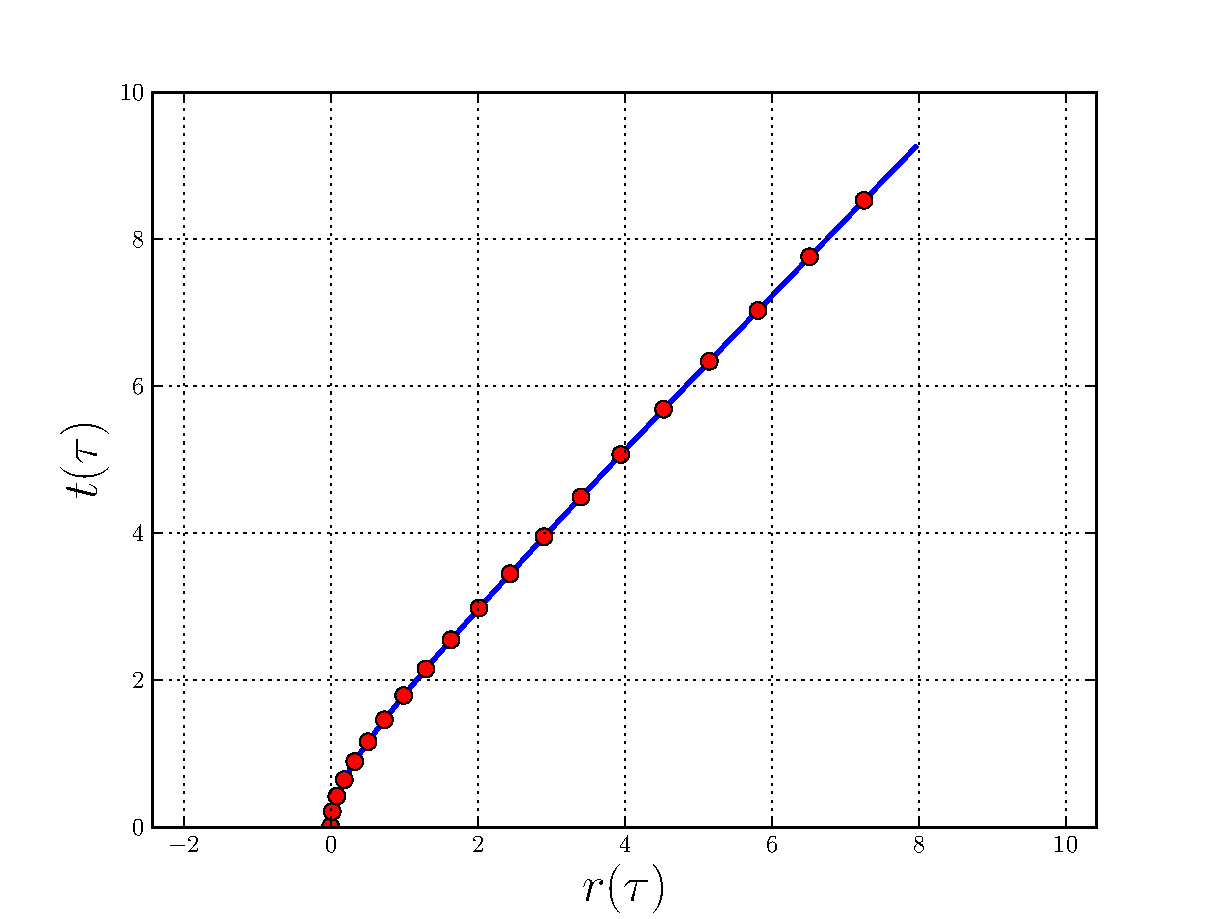
\includegraphics{minkowski.pdf}}
\caption{Expansion Radius of Model Universe, $\f{r}{\tau}$, where $\tau$ is the time coordinate.}
\end{center}
\end{figure} 
\begin{align*}
\deriv{r}{\tau} &= \tau \\
\deriv{t}{\tau} &= \sqrt{1+\tau^{2}} \\
\f{t}{\tau} &= \half\paren{\tau\sqrt{1+\tau^{2}}+\sinh^{-1}\tau}
\end{align*}
Spatial coordinates for the model universes are given by $\rho$ a spatial radius and the angular coordinates $\theta$ and $\phi$ if required. A
visualization of the 1-D spatial dimensional manifold is shown in figure~\ref{oneDU}.
\begin{sidewaysfigure}
\centering
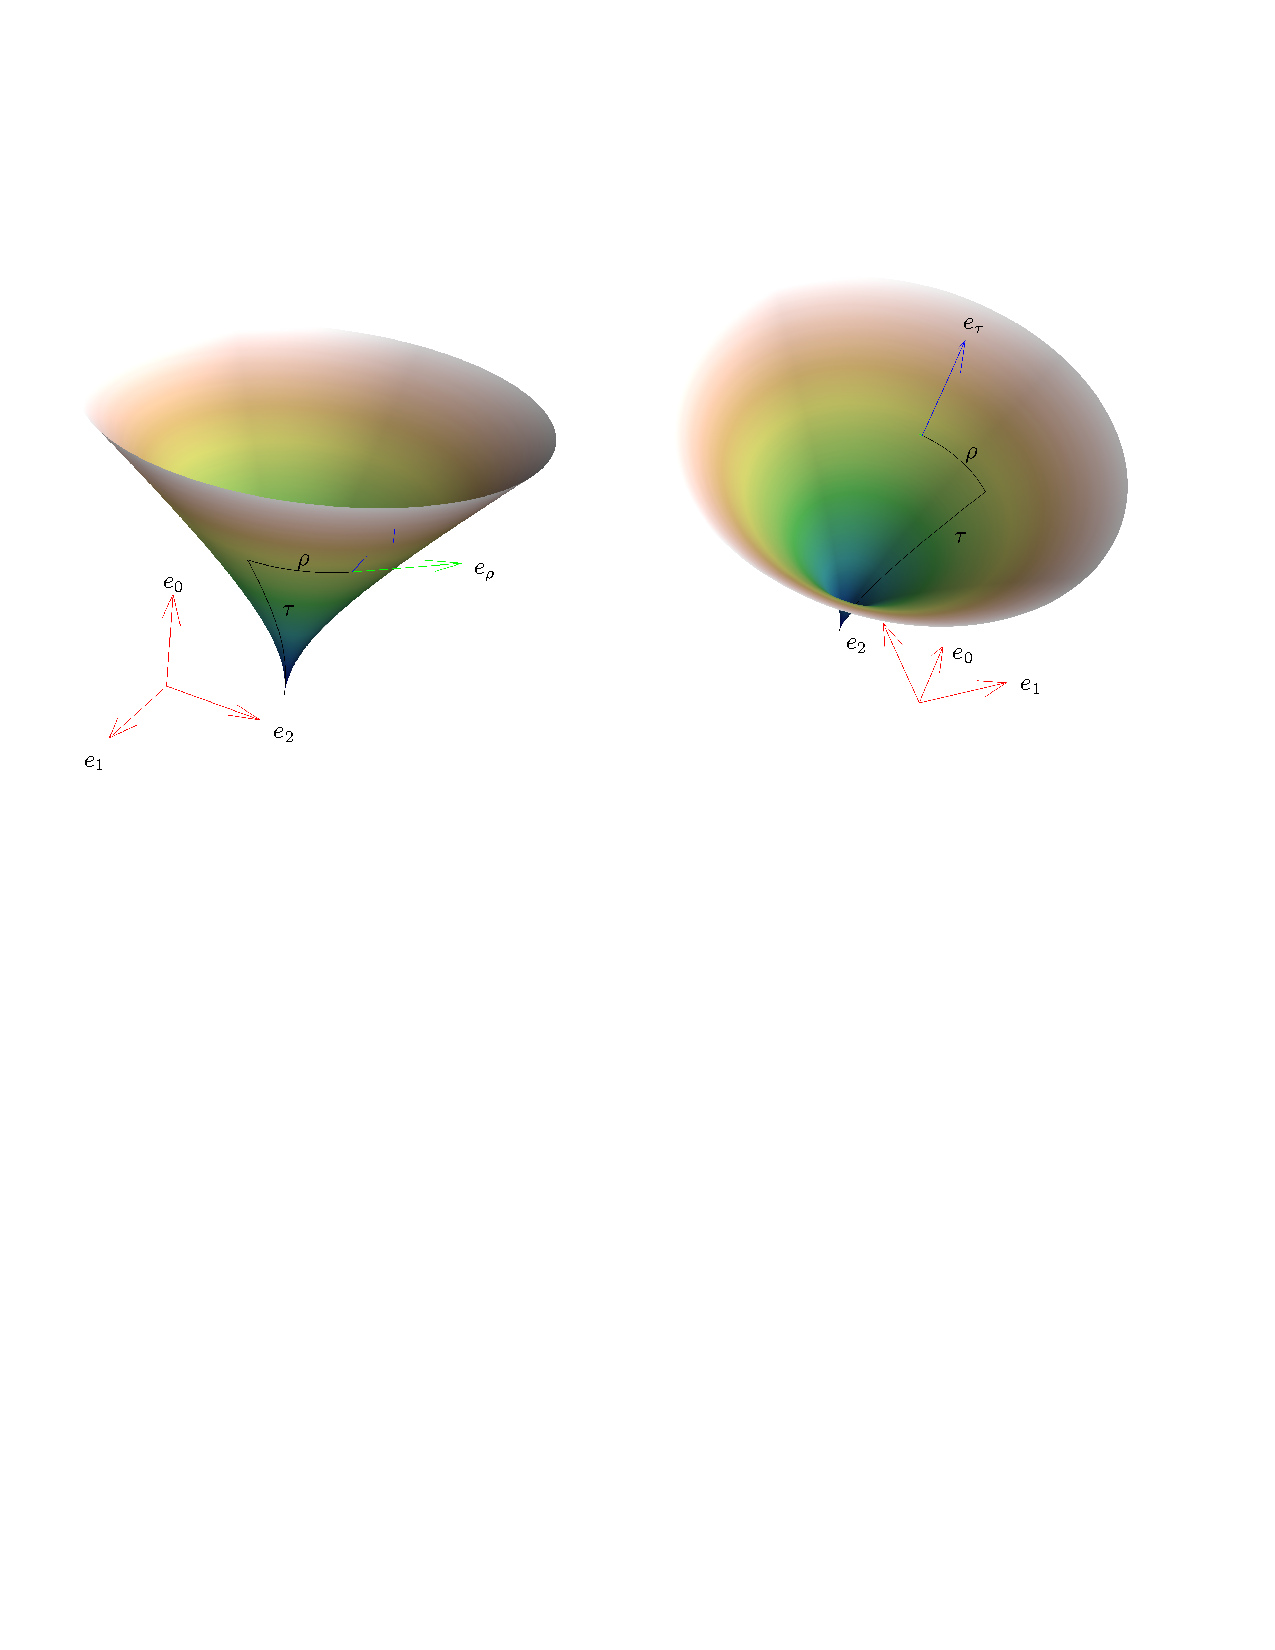
\includegraphics[clip=true,trim=0in 5in 0in 1in]{universe1d_tmp}
\caption[oneDU]{1D Universe}\label{oneDU}
\end{sidewaysfigure}
$e_{\tau}$ and $e_{\rho}$ are
\be
\begin{array}{ccc}
e_{\tau} = \pdiff{X^{(1)}}{\tau} & \mbox{ and } & e_{\rho} = \pdiff{X^{(1)}}{\rho}
\end{array}
\ee
and metric tensors for the three cases are
\be
g^{(i)}_{\mu\nu} = \pdiff{X^{(i)}}{\mu}\cdot\pdiff{X^{(i)}}{\nu}
\ee
where $\mu,\nu = \left \{ \tau,\rho,\theta,\phi \right \}$.  If we define $\f{h}{\tau,\rho}$ as
\be
 \f{h}{\tau,\rho} = \deriv{r}{\tau}\bfrac{\rho}{\f{r}{\tau}} 
\ee
Then the differential arclength given by the metric tensor, $g_{\mu\nu}$, is
\be
	\paren{ds}^{2} = g_{\mu\nu}dx^{\mu}dx^{\nu}
\ee
and the metric tensors for the three cases are (using sympy to do the algebra)
\be
g^{(1)}_{\mu\nu} = \lp
\begin{array}{cc}
1-h^{2} & h \\
h & -1 
\end{array}\rp
\ee
\be
g^{(2)}_{\mu\nu} = \lp
\begin{array}{ccc}
1-h^{2} & h & 0 \\
h & -1 & 0 \\
0 & 0 & -\paren{r\sinr}^{2} 
\end{array}\rp
\ee
\be
g^{(3)}_{\mu\nu} = \lp
\begin{array}{cccc}
1-h^{2} & h & 0 & 0 \\
h & -1 & 0 & 0 \\
0 & 0 & -\paren{r\sinr}^{2} & 0 \\
0 & 0 & 0 & -\paren{r\sinr\sin\theta}^{2} 
\end{array}\rp.
\ee
If we renormalize $e_{\theta}$ and $e_{\phi}$ to be unit vectors
\be
 e'_{\theta} = \bfrac{e_{\theta}}{\abs{r\sinr}} 
\ee
\be
 e'_{\phi} = \bfrac{e_{\phi}}{\abs{r\sinr\sin\theta}}
\ee
The metric tensors $g^{(2)}_{\mu\nu}$ and $g^{(3)}_{\mu\nu}$ become
\be
g'^{(2)}_{\mu\nu} = \lp
\begin{array}{ccc}
1-h^{2} & h & 0 \\
h & -1 & 0 \\
0 & 0 & -1 
\end{array}\rp
\ee
\be
g'^{(3)}_{\mu\nu} = \lp
\begin{array}{cccc}
1-h^{2} & h & 0 & 0 \\
h & -1 & 0 & 0 \\
0 & 0 & -1 & 0 \\
0 & 0 & 0 & -1 
\end{array}\rp
\ee
and
\be
\det\paren{g^{(1)}_{\mu\nu}} = \det\paren{g'^{(2)}_{\mu\nu}} = \det\paren{g'^{(3)}_{\mu\nu}} = -1 = I^{2}
\ee
For the 1-Dimensional space the differential arc length is
\be
 \paren{ds}^{2} = \paren{1-h^{2}}\paren{d\tau}^{2}+2hd\tau d\rho+\paren{d\rho}^{2}
\ee
so that for the light cone, $ds = 0$, we have the differential equation
\be
1-h^{2}+2h\deriv{\rho}{\tau}+\paren{\deriv{\rho}{\tau}}^{2} = 0
\ee
Note that this equation also applies to the 2 and 3 dimensional case if we set $\deriv{\theta}{\tau} = \deriv{\phi}{\tau} = 0$.  
Solving for $\deriv{\rho}{\tau}$ gives
\be\label{eq409}
	\deriv{\rho}{\tau} = h \pm 1 = \bfrac{1}{r}\deriv{r}{\tau}\rho \pm 1 = \paren{\deriv{}{\tau}\f{\ln}{r}}\rho \pm 1
\ee
Using the integration factor for linear first order differential equations the solution to equation ~\ref{eq409} is $\paren{\f{\rho}{\tau_{0}}=0}$
\be\label{eq407}
 \f{\rho}{\tau} = \pm \f{r}{\tau}\int_{\tau_{0}}^{\tau}\bfrac{d\tau'}{\f{r}{\tau'}}
\ee
Note that $\f{r}{\tau}$ and $\alpha\f{r}{\tau}$ have the same solution $\f{\rho}{\tau}$. Now consider the case that $\f{r}{\tau} = \tau^{\eta}$, then
\be
 \f{\rho}{\tau} = \pm\tau^{\eta}\int_{\tau_{0}}^{\tau} \paren{\tau'}^{-\eta}d\tau' = \lb 
\begin{array}{cc}
 \eta = 1, & \pm \tau\f{\ln}{\bfrac{\tau}{\tau_{0}}} \\
 \eta \neq 1, & \bfrac{\pm 1}{1-\eta}\paren{\tau-\tau_{0}\paren{\bfrac{\tau}{\tau_{0}}}^{\eta}} 
\end{array} 
  \rb
\ee
Typical $\f{\rho}{\tau}$'s for various $-1.5 \le \eta \le 1.5$ are shown in the light cone plot. If $\eta > 0$ the speed of light
is greater than $c$ in flat space.  If $\eta < 0$ the speed of light is less than $c$ in flat space. Note that if the universe is
curved, but not expanding or contracting the speed of light is the same as $c$ in flat space.

\begin{figure}[htbp]
\begin{center}
\scalebox{0.5}{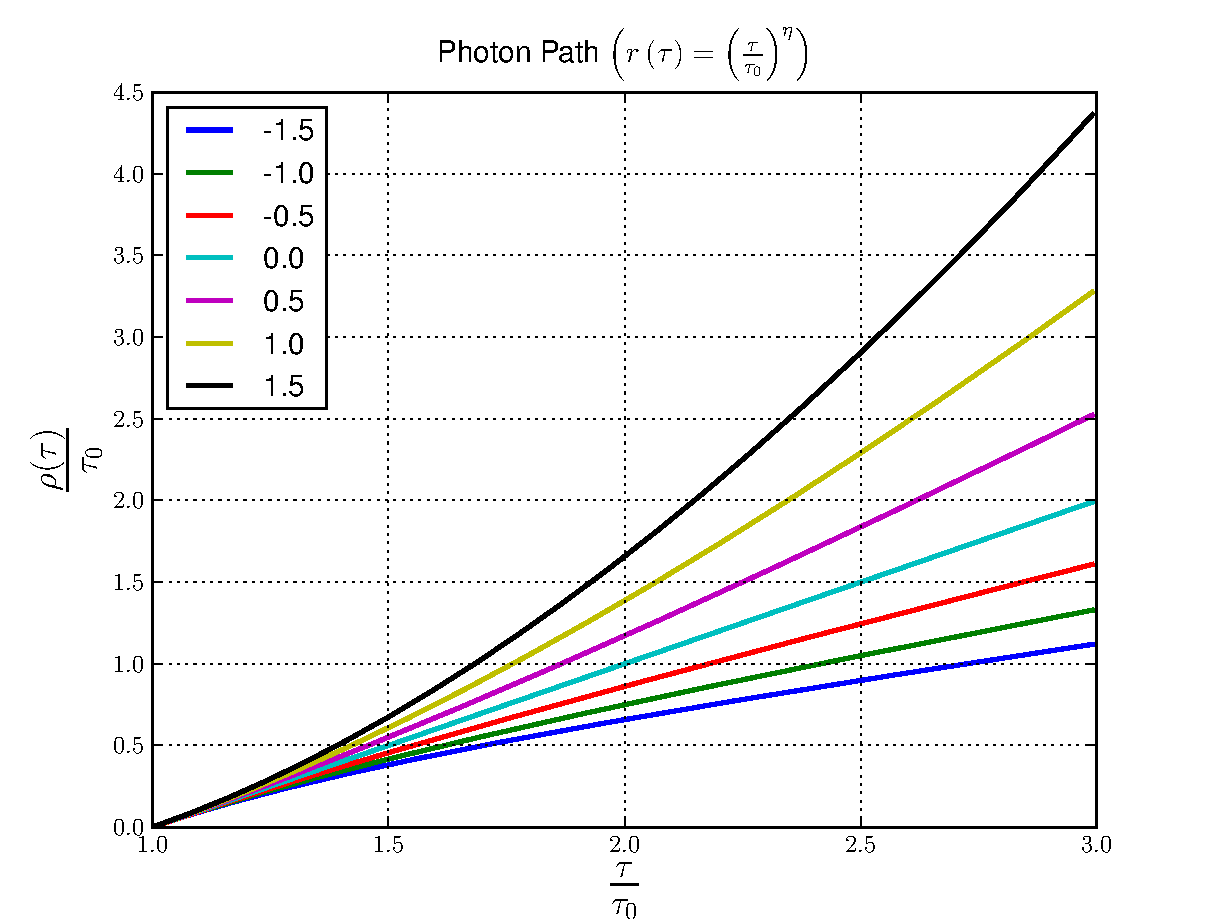
\includegraphics{lightcone.pdf}}
\caption{Lightcone in Curved Space}
\end{center}
\end{figure}
For a time periodic universe $\f{r}{\tau} = \f{\sin}{\bfrac{\tau}{T}}$ where $T$ is twice the period of the universe and $\f{\rho}{\tau_{0}}=0$, then
\be\label{eq412}
 \f{\rho}{\tau} = T\f{\sin}{\bfrac{\tau}{T}}\ln\abs{\bfrac{\f{\csc}{\bfrac{\tau_{0}}{T}}+\f{\cot}{\bfrac{\tau_{0}}{T}}}
                  {\f{\csc}{\bfrac{\tau}{T}}+\f{\cot}{\bfrac{\tau}{T}}}}
\ee
The plot of equation~\ref{eq412} is shown in figure~\ref{periodicU}
\begin{figure}[htbp]
\begin{center}
\scalebox{0.5}{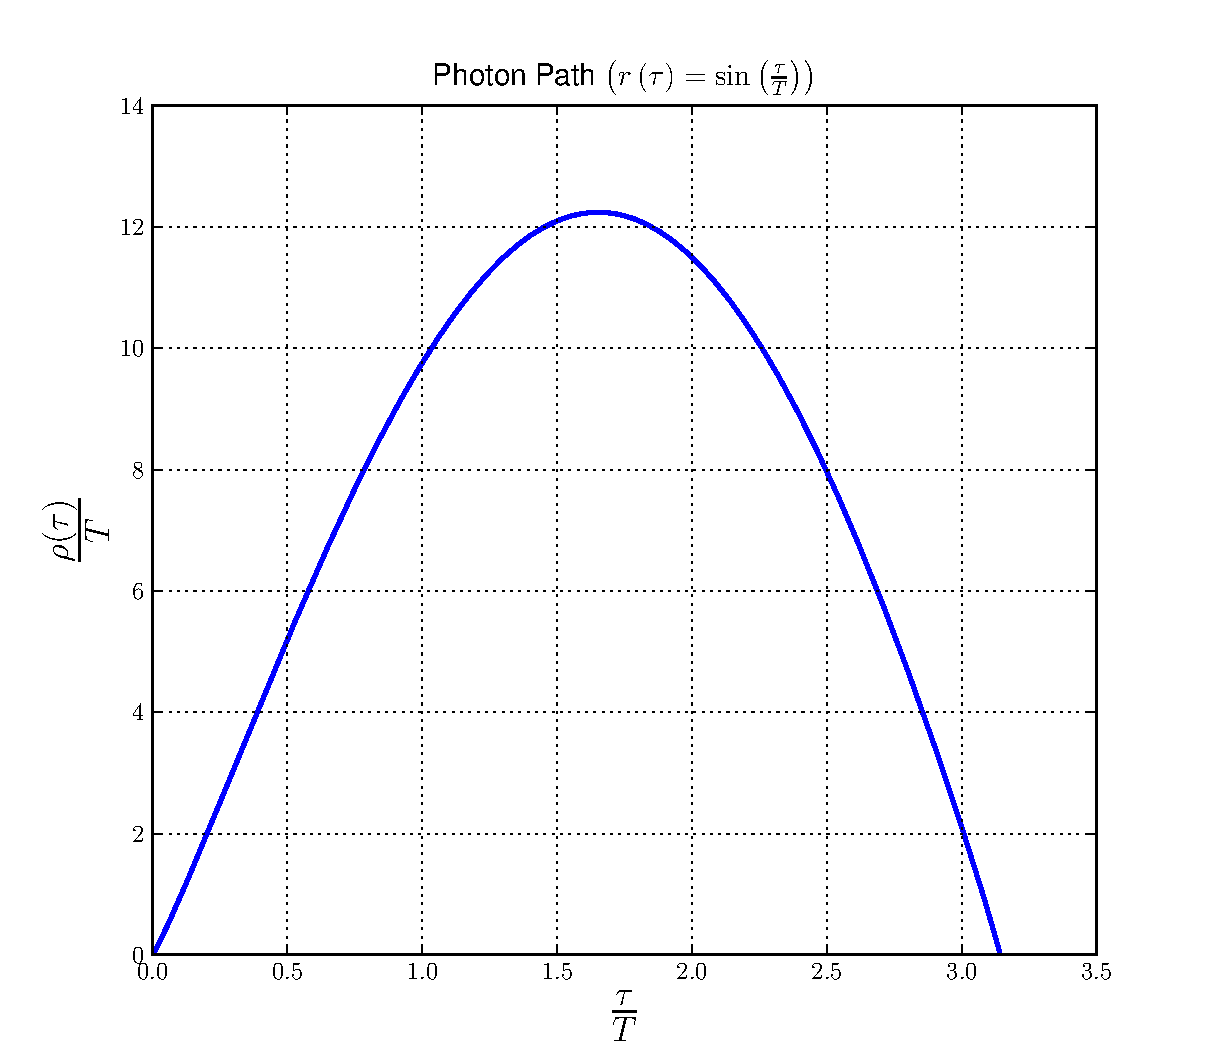
\includegraphics{periodiclightcone.pdf}}
\caption{Periodic Light Cone}\label{periodicU}
\end{center}
\end{figure}
\section{The Edge of Known Space}
Another kinematic question to answer is under what conditions light cannot access parts of the universe. The critical quantity is 
\be\label{eq410}
\f{\lambda}{\tau} = \bfrac{\f{\rho}{\tau}}{\vartheta\f{r}{\tau}}
\ee
where $\vartheta$ (the angular distance around the universe restricted to $0\le\vartheta\le\pi$) is the measure of how far from 
the observer you are. Since the universe is
spatially periodic the maximum value of $\vartheta$ is $\pi$.  If $\f{\lambda}{\tau} \ge 1$ for some finite $\tau$ you can access the 
distance defined by $\vartheta$.  Substituting equation~\ref{eq407} into equation~\ref{eq410} gives
\be
 \f{\lambda}{\tau} = \bfrac{1}{\vartheta}\int_{\tau_{0}}^{\tau}\bfrac{d\tau'}{\f{r}{\tau'}}
\ee
so that the connection condition is
\be
 \int_{\tau_{0}}^{\tau}\bfrac{d\tau'}{\f{r}{\tau'}} \ge \vartheta.
\ee
First consider a linear expansion model of the form 
\be
\f{r}{\tau} = r_{0}\paren{1+\alpha\paren{\bfrac{\tau}{\tau_{0}}-1}}
\ee
where $\f{r}{\tau_{0}} = r_{0}$.  Then
\be
\bfrac{\tau}{\tau_{0}} \ge \bfrac{1}{\alpha}e^{\alpha\vartheta\paren{\bfrac{r_{0}}{\tau_{0}}}}-1
\ee

In a linearly expanding universe the photon time of flight increases exponentially with distance. Now consider super-linear expansion of the form 
($\eta > 1$)
\be
\f{r}{\tau} = r_{0}\paren{1+\alpha\paren{\frac{\tau}{\tau_{0}}-1}^{\eta}}
\ee
Then
\be\label{eq416}
\bfrac{\tau_{0}}{r_{0}}\alpha^{-\frac{1}{\eta}}\int_{0}^{\alpha^{\frac{1}{\eta}}\paren{\frac{\tau}{\tau_{0}}-1}}\frac{d\mu}{1+\mu^{\eta}} \ge \vartheta,
\ee
but the integral in equation~\ref{eq416} does not have a closed form solution unless we let $\tau\rightarrow\infty$.  In that 
case\footnote{$\int_{0}^{\infty}\frac{dx}{1+x^{\eta}}$ is 3.241-2 in "Gradshteyn and Ryzhik"} we can write
\be\label{eq417}
\frac{1}{\eta}\alpha^{-\frac{1}{\eta}}\f{\csc}{\frac{\pi}{\eta}} \ge \paren{\frac{\vartheta}{\pi}}\paren{\frac{r_{0}}{\tau_{0}}}
\ee
A contour plot of the left side of equation~\ref{eq417} is shown below

\begin{figure}[htbp]
\begin{center}
\scalebox{0.5}{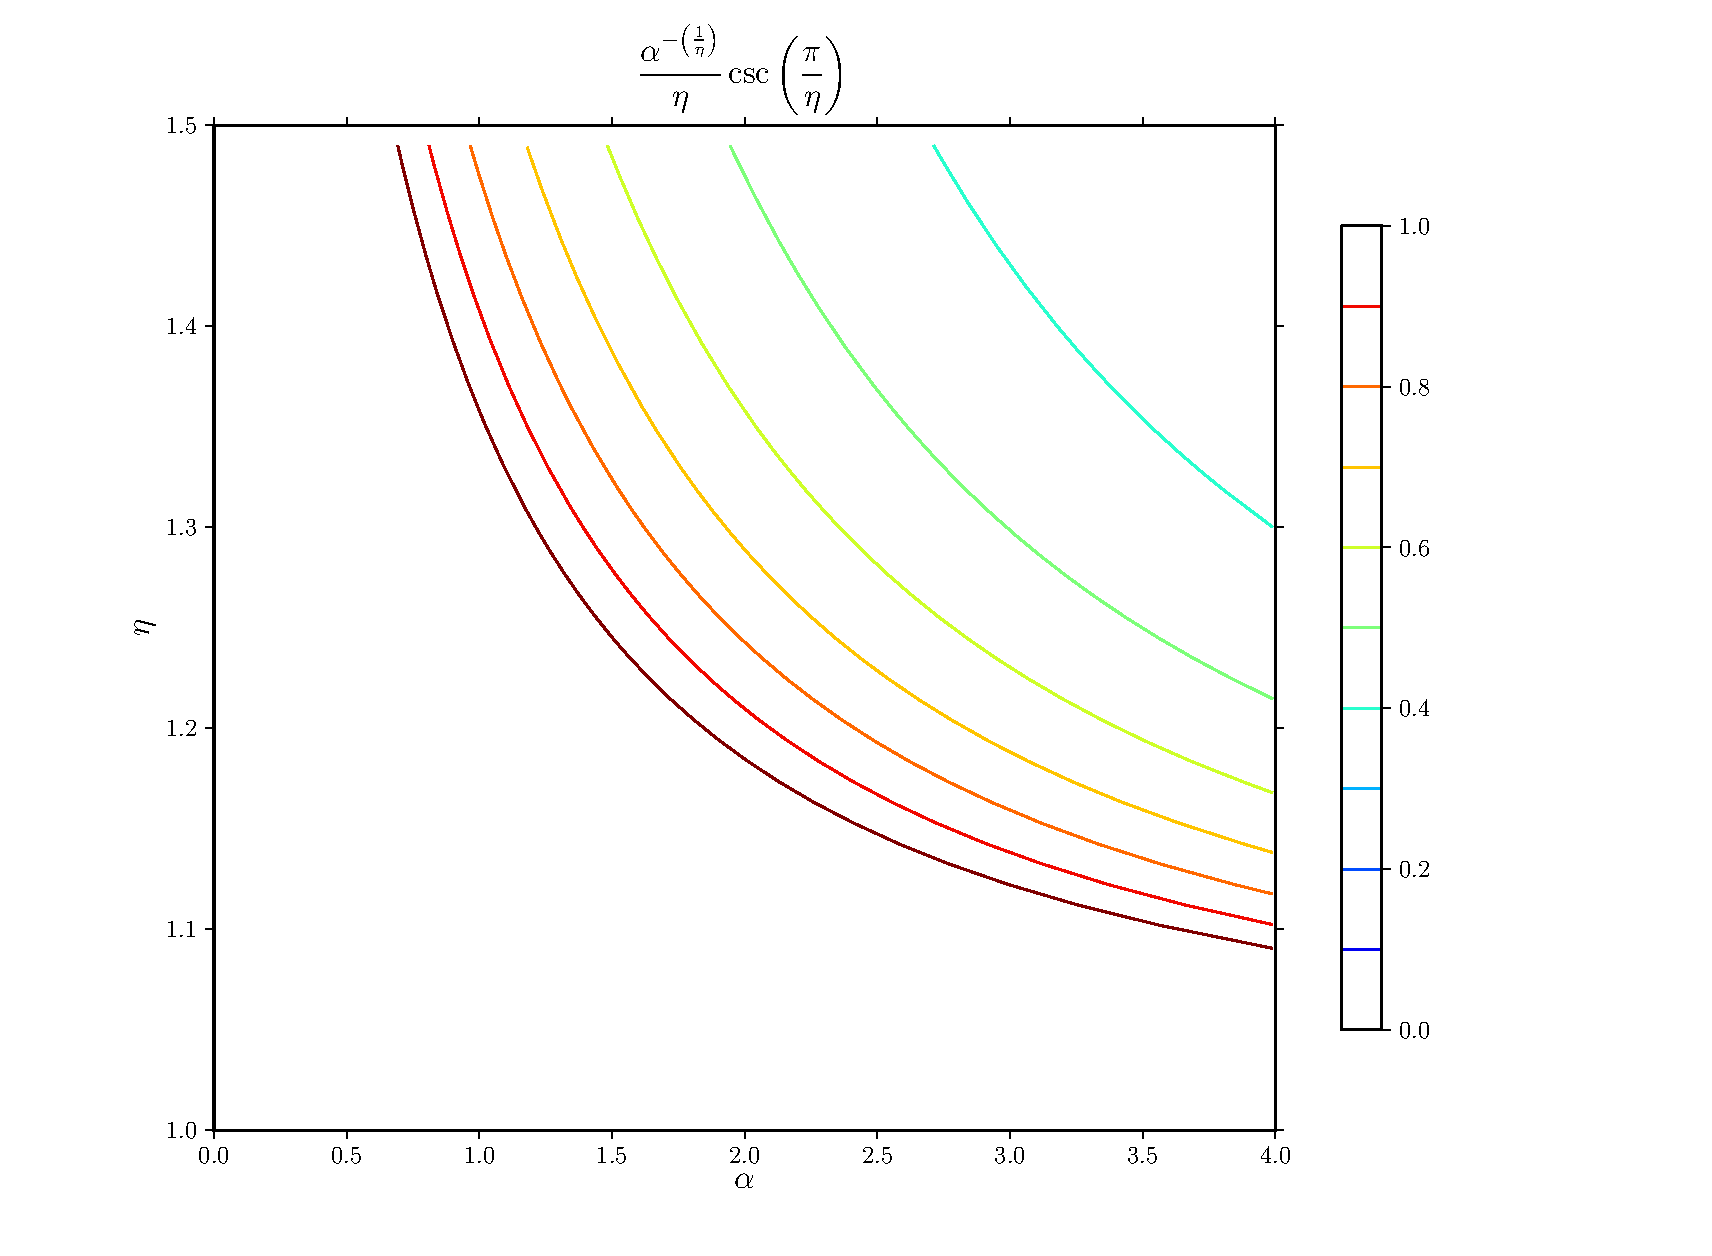
\includegraphics{exclusion.pdf}}
\caption{Photon Exclusion Zone}
\end{center}
\end{figure}
The right side of equation~\ref{eq417}, $\paren{\bfrac{\vartheta}{\pi}}\paren{\bfrac{r_{0}}{\tau_{0}}}$, is interpreted as follows -
\begin{enumerate}
 \item $\bfrac{\vartheta}{\pi}$ is the fractional distance around the closed spatially periodic universe. $\bfrac{\vartheta}{\pi}=1$ is as far as one can
 go before the distance from the observer starts to decrease.
 \item $\bfrac{r_{0}}{\tau_{0}}$ is a measure of inflation.  Immediately after an inflationary epoch $\bfrac{r_{0}}{\tau_{0}} >> 1$.
\end{enumerate}
Thus equation~\ref{eq417} determined the maximum distance $\bfrac{\vartheta}{\pi}$ that a photon can propagate in a finite amount of time.

Another question to consider is under what conditions $\bfrac{r_{0}}{\tau_{0}}$ will increase as $\tau_{0}$ increases or when will the
following be true
\be\label{eq418}
 \bfrac{\f{r}{\tau}}{\tau} \ge \bfrac{\f{r}{\tau_{0}}}{\tau_{0}} .
\ee
Equation~\ref{eq418} is equivalent to 
\be
 \alpha\paren{\bfrac{\tau}{\tau_{0}}-1}^{\eta-1} \ge 1
\ee
so that if $\eta >1$ then $\bfrac{\f{r}{\tau_{0}}}{\tau_{0}}$ will eventually grow as $\tau_{0}$ increases.


\begin{thebibliography}{99}
\bibitem {Cambridge} Cambridge site: \url{http://www.mrao.cam.ac.uk/~clifford}
\bibitem {AzSt} Arizona State site: \url{http://modelingnts.la.asu.edu}
\bibitem {D&L} Chris Doran and Anthony Lasenby, ``Geometric Algebra for Physicists,'' Cambridge University
Press, 2003.
\bibitem {H&S} David Hestenes and Garret Sobczyk, ``Clifford Algebra to Geometric Calculus,'' Kluwer Academic
Publishers, 1984.
\bibitem {DHS&VA} C. Doran,D. Hestenes, F. Sommen and N. Van Acker, ``Lie Groups as Spin Groups,'' 
	\emph{J. Math. Phys.},\textbf{ 34}(8) August 1993, pp. 3642-3669.
\bibitem {NFCM} David Hestenes, ``New Foundations for Classical Mechanics ($2^{nd}$ edition),'' Kluwer Academic
Publishers, 1999.
\bibitem {Wyss} Walter Wyss,``The Energy-Momentum Tensor in Classical Field Theory,'' \url{http://merlin.fic.uni.lodz.pl/concepts/2005_3_4/2005_3_4_295.pdf}
\end{thebibliography}
\end{document}
